%-------------------------------------------------------------------------------------
%\documentclass[a4paper, 11pt, oneside, openany]{ThesisStyle}
\documentclass[a4paper, 11pt, twoside, openany]{ThesisStyle}

%-------------------------------------------------------------------------------------
\usepackage{amsmath}
\usepackage{amssymb}
\usepackage{latexsym}
\usepackage{graphicx}
\usepackage{epsfig}
\usepackage{epstopdf}
\usepackage[dvipsnames]{xcolor}
\usepackage{url}
\usepackage{cite}
\usepackage[nottoc]{tocbibind}
\usepackage{multirow}
\usepackage[left=1.2in, right=1in, top=1in, bottom=1in, includefoot, headheight=13.6pt]{geometry}
\usepackage{array} %allow commands for the table columns specification
\usepackage{subfigure} %for column figures
\usepackage{floatflt} %for floating (wrapped) figures
\usepackage[british]{babel} % For british english hyphenation patterns
\usepackage[font=small, labelfont=bf]{caption} % Captions
\usepackage{url} % Formatting for URL's i.e. http://www.rhizobia.co.nz
\usepackage{microtype} % makes pdf look better
\usepackage[nottoc]{tocbibind} % Table of contents
\usepackage[hyperindex=true,pdftitle={Search for diboson resonances in the dijet final state with CMS},pdfauthor={Thea Klaeboe  Aarrestad},colorlinks=false,pagebackref=false,citecolor=blue,plainpages=false,filecolor=blue,linkcolor=blue,urlcolor=blue,pdfpagelabels]{hyperref} % colourlinks=false for printing 
\usepackage{xspace}
\usepackage{fancyhdr}
\usepackage{wrapfig}
\usepackage{afterpage}
%\usepackage{feynman}
%\usepackage[colorlinks=true,citecolor=blue,filecolor=blue,linkcolor=blue,urlcolor=blue,pdftex]{hyperref}
%\usepackage{capt-of} % needed to put table next to a figure and have captions
%\usepackage{natbib} % The best package for bibliographies
%\usepackage[width=11cm,font=footnotesize,labelfont=bf, format=default,justification=centerlast]{caption} % Captions\usepackage{fancyhdr} % Change caption style; changes headers and page styles etc.
%\usepackage{natbib}


\usepackage{titlesec}

\titleformat{\chapter}
{\color{CadetBlue}\normalfont\Large\bfseries}
{\color{CadetBlue}\thechapter}{1em}{}

\titleformat{\section}
{\color{CadetBlue}\normalfont\Large\bfseries}
{\color{CadetBlue}\thesection}{1em}{}

\titleformat{\subsection}
{\color{CadetBlue}\normalfont\Large\bfseries}
{\color{CadetBlue}\thesubsection}{1em}{}

\titleformat{\subsubsection}
{\color{CadetBlue}\normalfont\Large\bfseries}
{\color{CadetBlue}\thesubsection}{1em}{}

%-------------------------------------------------------------------------------------
\pagestyle{fancy}
% with this we ensure that the chapter and section
% headings are in lowercase.
\renewcommand{\chaptermark}[1]{\markboth{#1}{}}
\renewcommand{\sectionmark}[1]{\markright{\thesection\ #1}}
\fancyhf{} % delete current setting for header and footer
\fancyhead[LE,RO]{\bfseries\thepage}
\fancyhead[LO]{\bfseries\rightmark}
\fancyhead[RE]{\bfseries\leftmark}
%\renewcommand{\headrulewidth}{0.5pt}
%\renewcommand{\footrulewidth}{0pt}
\addtolength{\headheight}{0.5pt} % make space for the rule
%\fancypagestyle{plain}{%
%\fancyhead{} % get rid of headers on plain pages
%\renewcommand{\headrulewidth}{0pt} % and the line
%-------------------------------------------------------------------------------------

%-------------------------------------------------------------------------------------
\providecommand{\FIXME}[1]{\textcolor{red}{{\sffamily{\bfseries{}FIXME:} #1}}}

\newcommand{\mJ}{\ensuremath{m_{\text{jet}}}\xspace} 


%-------------------------------------------------------------------------------------
%%%%%%%%%%%%%%%%%%%%%%%%%%%%%%%%%%%%%%%%%%%%%%%%%%%%%%%%%%%%%%%%%%%%
%
%  Common definitions
%
%  N.B. use of \providecommand rather than \newcommand means
%       that a definition is ignored if already specified
%
%                                              L. Taylor 18 Feb 2005
%%%%%%%%%%%%%%%%%%%%%%%%%%%%%%%%%%%%%%%%%%%%%%%%%%%%%%%%%%%%%%%%%%%%
% PRIVATE
\newcommand{\mVV}{\ensuremath{m_{\VV}}\xspace}
\newcommand{\mqV}{\ensuremath{m_{\qo\PV}}\xspace}
\newcommand{\mjj}{\ensuremath{m_\mathrm{jj}}}
\newcommand{\mJ}{\ensuremath{m_{\text{jet}}}}
\newcommand{\nsubj}{\ensuremath{\tau_{21}}}
\newcommand{\ddt}{\ensuremath{\tau_{21}^{DDT}}}
\newcommand{\ktilde}{\ensuremath{\tilde{k}}}
\newcommand{\VV}{\ensuremath{\PV\PV}\xspace}
\newcommand{\WW}{\ensuremath{\PW\PW}\xspace}
\newcommand{\WZ}{\ensuremath{\PW\PZ}\xspace}
\newcommand{\ZZ}{\ensuremath{\PZ\PZ}\xspace}
\newcommand{\mX}{\ensuremath{\text{M}_{\text{X}}}}%
% Some shorthand
% turn off italics
\newcommand {\etal}{\mbox{et al.}\xspace} %et al. - no preceding comma
\newcommand {\ie}{\mbox{i.e.}\xspace}     %i.e.
\newcommand {\eg}{\mbox{e.g.}\xspace}     %e.g.
\newcommand {\etc}{\mbox{etc.}\xspace}     %etc.
\newcommand {\vs}{\mbox{\sl vs.}\xspace}      %vs.
\newcommand {\mdash}{\ensuremath{\mathrm{-}}} % for use within formulas

% some terms whose definition we may change
\newcommand {\Lone}{Level-1\xspace} % Level-1 or L1 ?
\newcommand {\Ltwo}{Level-2\xspace}
\newcommand {\Lthree}{Level-3\xspace}

% Some software programs (alphabetized)
\providecommand{\ACERMC} {\textsc{AcerMC}\xspace}
\newcommand{\amcatnlo}{\textsc{madgraph5\_amc@nlo}\xspace}
\providecommand{\ALPGEN} {{\textsc{alpgen}}\xspace}
\providecommand{\CHARYBDIS} {{\textsc{charybdis}}\xspace}
\providecommand{\CMKIN} {\textsc{cmkin}\xspace}
\providecommand{\CMSIM} {{\textsc{cmsim}}\xspace}
\providecommand{\CMSSW} {{\textsc{cmssw}}\xspace}
\providecommand{\COBRA} {{\textsc{cobra}}\xspace}
\providecommand{\COCOA} {{\textsc{cocoa}}\xspace}
\providecommand{\COMPHEP} {\textsc{CompHEP}\xspace}
\providecommand{\EVTGEN} {{\textsc{evtgen}}\xspace}
\providecommand{\FAMOS} {{\textsc{famos}}\xspace}
\providecommand{\GARCON} {\textsc{garcon}\xspace}
\providecommand{\GARFIELD} {{\textsc{garfield}}\xspace}
\providecommand{\GEANE} {{\textsc{geane}}\xspace}
\providecommand{\GEANTfour} {{\textsc{geant4}}\xspace}
\providecommand{\GEANTthree} {{\textsc{geant3}}\xspace}
\providecommand{\GEANT} {{\textsc{geant}}\xspace}
\providecommand{\HDECAY} {\textsc{hdecay}\xspace}
\providecommand{\HERWIG} {{\textsc{herwig}}\xspace}
\providecommand{\HIGLU} {{\textsc{higlu}}\xspace}
\providecommand{\HIJING} {{\textsc{hijing}}\xspace}
\providecommand{\IGUANA} {\textsc{iguana}\xspace}
\providecommand{\ISAJET} {{\textsc{isajet}}\xspace}
\providecommand{\ISAPYTHIA} {{\textsc{isapythia}}\xspace}
\providecommand{\ISASUGRA} {{\textsc{isasugra}}\xspace}
\providecommand{\ISASUSY} {{\textsc{isasusy}}\xspace}
\providecommand{\ISAWIG} {{\textsc{isawig}}\xspace}
\providecommand{\MADGRAPH} {\textsc{MadGraph}\xspace}
\providecommand{\MCATNLO} {\textsc{mc@nlo}\xspace}
\providecommand{\MCFM} {\textsc{mcfm}\xspace}
\providecommand{\MILLEPEDE} {{\textsc{millepede}}\xspace}
\providecommand{\ORCA} {{\textsc{orca}}\xspace}
\providecommand{\OSCAR} {{\textsc{oscar}}\xspace}
\providecommand{\PHOTOS} {\textsc{photos}\xspace}
\providecommand{\POWHEG} {{\textsc{powheg}}\xspace}
\providecommand{\PROSPINO} {\textsc{prospino}\xspace}
\providecommand{\PYTHIA} {{\textsc{pythia}}\xspace}
\providecommand{\SHERPA} {{\textsc{sherpa}}\xspace}
\providecommand{\TAUOLA} {\textsc{tauola}\xspace}
\providecommand{\TOPREX} {\textsc{TopReX}\xspace}
\providecommand{\XDAQ} {{\textsc{xdaq}}\xspace}

%%%%%%%%%% Experiments %%%%%%%%%%%%%%%%%%

\newcommand {\DZERO}{D\O\xspace}     %etc.

%%%%%%%%%% Measurements and units %%%%%%%%%%%%%%%%%%

\newcommand{\de}{\ensuremath{^\circ}\xspace}
\newcommand{\ten}[1]{\ensuremath{\times \text{10}^\text{#1}}}
\newcommand{\unit}[1]{\ensuremath{\text{\,#1}}\xspace}
\newcommand{\mum}{\ensuremath{\,\mu\text{m}}\xspace}
\newcommand{\micron}{\ensuremath{\,\mu\text{m}}\xspace}
\newcommand{\cm}{\ensuremath{\,\text{cm}}\xspace}
\newcommand{\mm}{\ensuremath{\,\text{mm}}\xspace}
\newcommand{\mus}{\ensuremath{\,\mu\text{s}}\xspace}
\newcommand{\keV}{\ensuremath{\,\text{ke\hspace{-.08em}V}}\xspace}
\newcommand{\MeV}{\ensuremath{\,\text{Me\hspace{-.08em}V}}\xspace}
\newcommand{\GeV}{\ensuremath{\,\text{Ge\hspace{-.08em}V}}\xspace}
\newcommand{\TeV}{\ensuremath{\,\text{Te\hspace{-.08em}V}}\xspace}
\newcommand{\PeV}{\ensuremath{\,\text{Pe\hspace{-.08em}V}}\xspace}
\newcommand{\keVc}{\ensuremath{{\,\text{ke\hspace{-.08em}V\hspace{-0.16em}/\hspace{-0.08em}}c}}\xspace}
\newcommand{\MeVc}{\ensuremath{{\,\text{Me\hspace{-.08em}V\hspace{-0.16em}/\hspace{-0.08em}}c}}\xspace}
\newcommand{\GeVc}{\ensuremath{{\,\text{Ge\hspace{-.08em}V\hspace{-0.16em}/\hspace{-0.08em}}c}}\xspace}
\newcommand{\TeVc}{\ensuremath{{\,\text{Te\hspace{-.08em}V\hspace{-0.16em}/\hspace{-0.08em}}c}}\xspace}
\newcommand{\keVcc}{\ensuremath{{\,\text{ke\hspace{-.08em}V\hspace{-0.16em}/\hspace{-0.08em}}c^\text{2}}}\xspace}
\newcommand{\MeVcc}{\ensuremath{{\,\text{Me\hspace{-.08em}V\hspace{-0.16em}/\hspace{-0.08em}}c^\text{2}}}\xspace}
\newcommand{\GeVcc}{\ensuremath{{\,\text{Ge\hspace{-.08em}V\hspace{-0.16em}/\hspace{-0.08em}}c^\text{2}}}\xspace}
\newcommand{\TeVcc}{\ensuremath{{\,\text{Te\hspace{-.08em}V\hspace{-0.16em}/\hspace{-0.08em}}c^\text{2}}}\xspace}
\newcommand{\MPl}{\ensuremath{M_\mathrm{Pl}}\xspace}
\newcommand{\bMPl}{\ensuremath{\overline{M}_\mathrm{Pl}}\xspace}

\newcommand{\pbinv} {\mbox{\ensuremath{\,\text{pb}^\text{$-$1}}}\xspace}
\newcommand{\fbinv} {\mbox{\ensuremath{\,\text{fb}^\text{$-$1}}}\xspace}
\newcommand{\nbinv} {\mbox{\ensuremath{\,\text{nb}^\text{$-$1}}}\xspace}
\newcommand{\percms}{\ensuremath{\,\text{cm}^\text{$-$2}\,\text{s}^\text{$-$1}}\xspace}
\newcommand{\lumi}{\ensuremath{\mathcal{L}}\xspace}
\newcommand{\Lumi}{\ensuremath{\mathcal{L}}\xspace}%both upper and lower
%
% Need a convention here:
\newcommand{\LvLow}  {\ensuremath{\mathcal{L}=\text{10}^\text{32}\,\text{cm}^\text{$-$2}\,\text{s}^\text{$-$1}}\xspace}
\newcommand{\LLow}   {\ensuremath{\mathcal{L}=\text{10}^\text{33}\,\text{cm}^\text{$-$2}\,\text{s}^\text{$-$1}}\xspace}
\newcommand{\lowlumi}{\ensuremath{\mathcal{L}=\text{2}\times \text{10}^\text{33}\,\text{cm}^\text{$-$2}\,\text{s}^\text{$-$1}}\xspace}
\newcommand{\LMed}   {\ensuremath{\mathcal{L}=\text{2}\times \text{10}^\text{33}\,\text{cm}^\text{$-$2}\,\text{s}^\text{$-$1}}\xspace}
\newcommand{\LHigh}  {\ensuremath{\mathcal{L}=\text{10}^\text{34}\,\text{cm}^\text{$-$2}\,\text{s}^\text{$-$1}}\xspace}
\newcommand{\hilumi} {\ensuremath{\mathcal{L}=\text{10}^\text{34}\,\text{cm}^\text{$-$2}\,\text{s}^\text{$-$1}}\xspace}


%%%%%%%%%% Some usual physics terms/symbols %%%%%%%%%%%%%%%%%%

\newcommand{\kt}{\ensuremath{k_{\mathrm{T}}}\xspace}
\newcommand{\wangle}{\ensuremath{\sin^{2}\theta_{\text{eff}}^\text{lept}(M^2_\mathrm{Z})}\xspace}
\newcommand{\stat}{\ensuremath{\,\text{(stat.)}}\xspace}
\newcommand{\syst}{\ensuremath{\,\text{(syst.)}}\xspace}
\newcommand{\AFB}{\ensuremath{A_\text{FB}}\xspace}
\newcommand{\MD}{\ensuremath{{M_\mathrm{D}}}\xspace}% ED mass
\newcommand{\Mpl}{\ensuremath{{M_\mathrm{Pl}}}\xspace}% Planck mass
\newcommand{\Rinv} {\ensuremath{{R}^{-1}}\xspace}

\providecommand{\Em}{\ensuremath{E\hspace{-0.6em}/}\xspace}
\providecommand{\Pm}{\ensuremath{p\hspace{-0.5em}/}\xspace}
\providecommand{\PTm}{\ensuremath{{p}_\mathrm{T}\hspace{-1.02em}/}\xspace}
\newcommand{\PT}{\ensuremath{p_{\mathrm{T}}}\xspace}
\newcommand{\pt}{\ensuremath{p_{\mathrm{T}}}\xspace}
\newcommand{\Vpt}{\ensuremath{{\vec p}_{\mathrm{T}}}\xspace}
\newcommand{\ET}{\ensuremath{E_{\mathrm{T}}}\xspace}
\newcommand{\et}{\ensuremath{E_{\mathrm{T}}}\xspace}
\newcommand{\HT}{\ensuremath{H_{\mathrm{T}}}\xspace}
\newcommand{\Etmiss}{\ensuremath{E_{\mathrm{T}\!{\rm miss}}}}
\newcommand{\ETm}{\ensuremath{E_{\mathrm{T}}^{\text{miss}}}\xspace}
\newcommand{\MET}{\ensuremath{E_{\mathrm{T}}^{\text{miss}}}\xspace}
\newcommand{\ETmiss}{\ensuremath{E_{\mathrm{T}}^{\text{miss}}}\xspace}
\newcommand{\VEtmiss}{\ensuremath{{\vec E}_{\mathrm{T}}^{\;\text{miss}}}\xspace}
\newcommand{\ptvecmiss}{\ensuremath{{\vec p}_{\mathrm{T}}^{\kern1pt\text{miss}}}\xspace}
\providecommand{\PTslash}{\ensuremath{{p}_\mathrm{T}\hspace{-1.02em}/}\xspace}
\providecommand{\ETslash}{\ensuremath{E_{\mathrm{T}}\hspace{-1.1em}/}\xspace}

%%%%%%%%%% SM particles %%%%%%%%%%%%%%%%%%

\newcommand{\BC}{\ensuremath{{B_{\mathrm{c}}}}\xspace}
\newcommand{\JPsi}{\ensuremath{{J}\hspace{-.08em}/\hspace{-.14em}\psi}\xspace}
\providecommand{\cPJgy}{\JPsi} % J/Psi (no mass)
\newcommand{\bspsiphi}{\ensuremath{B_s \to \JPsi\, \phi}\xspace}
\providecommand{\JPsi}{\ensuremath{\mathrm{J}\hspace{-.08em}/\hspace{-.14em}\psi}\xspace}

%quarks
\newcommand{\cPg}{\ensuremath{\mathrm{g}}} % generic gluon
\newcommand{\cPq}{\ensuremath{\mathrm{q}}}
\newcommand{\cPaq}{\ensuremath{\overline{\mathrm{q}}}}
\newcommand{\qqbarpr}{\ensuremath{\cPq\cPaq^({}'^){}}\xspace}
\newcommand{\qqbar}{\ensuremath{\cPq\cPaq}\xspace}
\newcommand{\cPqt}{\ensuremath{\mathrm{t}}} % t for t quark
\newcommand{\cPqb}{\ensuremath{\mathrm{b}}} % b for b quark
\newcommand{\bbarc}{\ensuremath{{\overline{b}c}}\xspace}
\newcommand{\bbbar}{\ensuremath{{\mathrm{b}\overline{\mathrm{b}}}}\xspace}
\newcommand{\ccbar}{\ensuremath{{c\overline{c}}}\xspace}
\providecommand{\ttbar}{\ensuremath{\mathrm{t}\overline{\mathrm{t}}}\xspace}

%leptons/neutrinos
\newcommand{\Pgn}{\ensuremath{\nu}}%neutrino
\providecommand{\cPgn}{\ensuremath{\nu}\xspace} % generic neutrino
\newcommand{\EE}{\ensuremath{e^+e^-}\xspace}
\newcommand{\MM}{\ensuremath{\mu^+\mu^-}\xspace}
\newcommand{\TT}{\ensuremath{\tau^+\tau^-}\xspace}

%bosons
\providecommand{\PZ}{\ensuremath{\mathrm{Z}}\xspace}
\providecommand{\cPZ}{\Z} % plain Z (no superscript 0)
\providecommand{\PW}{\ensuremath{\mathrm{W}}\xspace}
\providecommand{\PV}{\ensuremath{\mathrm{V}}\xspace}
\providecommand{\PH}{\ensuremath{\mathrm{H}}\xspace}
\providecommand{\PWL}{\ensuremath{\mathrm{W}_{\mathrm{L}}}\xspace}
\providecommand{\PWT}{\ensuremath{\mathrm{W}_{\mathrm{T}}}\xspace}

%%%%%%%%%% BSM particles %%%%%%%%%%%%%%%%%%

\providecommand{\Zpr}{\ensuremath{\mathrm{Z}^\prime}\xspace}
\providecommand{\cPZpr}{\Zpr} % plain Z'
\providecommand{\PZpr}{\ensuremath{\mathrm{Z}^\prime}\xspace} % plain Z' using prime
\providecommand{\Wpr}{\ensuremath{\mathrm{W}^\prime}\xspace}
\providecommand{\cPWpr}{\Wpr} % plain W'
\providecommand{\PWpr}{\ensuremath{\mathrm{W}^\prime}\xspace} % plain W' using prime
\providecommand{\PVpr}{\ensuremath{\mathrm{V}^\prime}\xspace} % plain V' using prime
\providecommand{\BulkG}{\ensuremath{\mathrm{G}_\mathrm{bulk}}\xspace}

%%%%%%%%%%%%%  E-gamma definitions %%%%%%%%%%%%%%
\newcommand{\HGG}{\ensuremath{\mathrm{H}\to\gamma\gamma}}
\newcommand{\gev}{\GeV}
\newcommand{\GAMJET}{\ensuremath{\gamma + \text{jet}}}
\newcommand{\PPTOJETS}{\ensuremath{\mathrm{pp}\to\text{jets}}}
\newcommand{\PPTOGG}{\ensuremath{\mathrm{pp}\to\gamma\gamma}}
\newcommand{\PPTOGAMJET}{\ensuremath{\mathrm{pp}\to\gamma + \mathrm{jet}}}
\newcommand{\MH}{\ensuremath{\mathrm{M_{\mathrm{H}}}}}
\newcommand{\RNINE}{\ensuremath{\mathrm{R}_\mathrm{9}}}
\newcommand{\DR}{\ensuremath{\Delta\mathrm{R}}}

%%%%%%%%%%%%%%% other stuff %%%%%%%%%%%%
\providecommand{\dd}[2]{\ensuremath{\frac{\mathrm{d} #1}{\mathrm{d} #2}}}

\newcommand{\ga}{\ensuremath{\gtrsim}}
\newcommand{\la}{\ensuremath{\lesssim}}
\newcommand{\swsq}{\ensuremath{\sin^2\theta_W}\xspace}
\newcommand{\cwsq}{\ensuremath{\cos^2\theta_W}\xspace}
\newcommand{\tanb}{\ensuremath{\tan\beta}\xspace}
\newcommand{\tanbsq}{\ensuremath{\tan^{2}\beta}\xspace}
\newcommand{\sidb}{\ensuremath{\sin 2\beta}\xspace}
\newcommand{\alpS}{\ensuremath{\alpha_S}\xspace}
\newcommand{\alpt}{\ensuremath{\tilde{\alpha}}\xspace}

\newcommand{\QL}{\ensuremath{Q_L}\xspace}
\newcommand{\sQ}{\ensuremath{\tilde{Q}}\xspace}
\newcommand{\sQL}{\ensuremath{\tilde{Q}_L}\xspace}
\newcommand{\ULC}{\ensuremath{U_L^C}\xspace}
\newcommand{\sUC}{\ensuremath{\tilde{U}^C}\xspace}
\newcommand{\sULC}{\ensuremath{\tilde{U}_L^C}\xspace}
\newcommand{\DLC}{\ensuremath{D_L^C}\xspace}
\newcommand{\sDC}{\ensuremath{\tilde{D}^C}\xspace}
\newcommand{\sDLC}{\ensuremath{\tilde{D}_L^C}\xspace}
\newcommand{\LL}{\ensuremath{L_L}\xspace}
\newcommand{\sL}{\ensuremath{\tilde{L}}\xspace}
\newcommand{\sLL}{\ensuremath{\tilde{L}_L}\xspace}
\newcommand{\ELC}{\ensuremath{E_L^C}\xspace}
\newcommand{\sEC}{\ensuremath{\tilde{E}^C}\xspace}
\newcommand{\sELC}{\ensuremath{\tilde{E}_L^C}\xspace}
\newcommand{\sEL}{\ensuremath{\tilde{E}_L}\xspace}
\newcommand{\sER}{\ensuremath{\tilde{E}_R}\xspace}
\newcommand{\sFer}{\ensuremath{\tilde{f}}\xspace}
\newcommand{\sQua}{\ensuremath{\tilde{q}}\xspace}
\newcommand{\sUp}{\ensuremath{\tilde{u}}\xspace}
\newcommand{\suL}{\ensuremath{\tilde{u}_L}\xspace}
\newcommand{\suR}{\ensuremath{\tilde{u}_R}\xspace}
\newcommand{\sDw}{\ensuremath{\tilde{d}}\xspace}
\newcommand{\sdL}{\ensuremath{\tilde{d}_L}\xspace}
\newcommand{\sdR}{\ensuremath{\tilde{d}_R}\xspace}
\newcommand{\sTop}{\ensuremath{\tilde{t}}\xspace}
\newcommand{\stL}{\ensuremath{\tilde{t}_L}\xspace}
\newcommand{\stR}{\ensuremath{\tilde{t}_R}\xspace}
\newcommand{\stone}{\ensuremath{\tilde{t}_1}\xspace}
\newcommand{\sttwo}{\ensuremath{\tilde{t}_2}\xspace}
\newcommand{\sBot}{\ensuremath{\tilde{b}}\xspace}
\newcommand{\sbL}{\ensuremath{\tilde{b}_L}\xspace}
\newcommand{\sbR}{\ensuremath{\tilde{b}_R}\xspace}
\newcommand{\sbone}{\ensuremath{\tilde{b}_1}\xspace}
\newcommand{\sbtwo}{\ensuremath{\tilde{b}_2}\xspace}
\newcommand{\sLep}{\ensuremath{\tilde{l}}\xspace}
\newcommand{\sLepC}{\ensuremath{\tilde{l}^C}\xspace}
\newcommand{\sEl}{\ensuremath{\tilde{e}}\xspace}
\newcommand{\sElC}{\ensuremath{\tilde{e}^C}\xspace}
\newcommand{\seL}{\ensuremath{\tilde{e}_L}\xspace}
\newcommand{\seR}{\ensuremath{\tilde{e}_R}\xspace}
\newcommand{\snL}{\ensuremath{\tilde{\nu}_L}\xspace}
\newcommand{\sMu}{\ensuremath{\tilde{\mu}}\xspace}
\newcommand{\sNu}{\ensuremath{\tilde{\nu}}\xspace}
\newcommand{\sTau}{\ensuremath{\tilde{\tau}}\xspace}
\newcommand{\Glu}{\ensuremath{g}\xspace}
\newcommand{\sGlu}{\ensuremath{\tilde{g}}\xspace}
\newcommand{\Wpm}{\ensuremath{W^{\pm}}\xspace}
\newcommand{\sWpm}{\ensuremath{\tilde{W}^{\pm}}\xspace}
\newcommand{\Wz}{\ensuremath{W^{0}}\xspace}
\newcommand{\sWz}{\ensuremath{\tilde{W}^{0}}\xspace}
\newcommand{\sWino}{\ensuremath{\tilde{W}}\xspace}
\newcommand{\Bz}{\ensuremath{B^{0}}\xspace}
\newcommand{\sBz}{\ensuremath{\tilde{B}^{0}}\xspace}
\newcommand{\sBino}{\ensuremath{\tilde{B}}\xspace}
\newcommand{\Zz}{\ensuremath{Z^{0}}\xspace}
\newcommand{\sZino}{\ensuremath{\tilde{Z}^{0}}\xspace}
\newcommand{\sGam}{\ensuremath{\tilde{\gamma}}\xspace}
\newcommand{\chiz}{\ensuremath{\tilde{\chi}^{0}}\xspace}
\newcommand{\chip}{\ensuremath{\tilde{\chi}^{+}}\xspace}
\newcommand{\chim}{\ensuremath{\tilde{\chi}^{-}}\xspace}
\newcommand{\chipm}{\ensuremath{\tilde{\chi}^{\pm}}\xspace}
\newcommand{\Hone}{\ensuremath{H_{d}}\xspace}
\newcommand{\sHone}{\ensuremath{\tilde{H}_{d}}\xspace}
\newcommand{\Htwo}{\ensuremath{H_{u}}\xspace}
\newcommand{\sHtwo}{\ensuremath{\tilde{H}_{u}}\xspace}
\newcommand{\sHig}{\ensuremath{\tilde{H}}\xspace}
\newcommand{\sHa}{\ensuremath{\tilde{H}_{a}}\xspace}
\newcommand{\sHb}{\ensuremath{\tilde{H}_{b}}\xspace}
\newcommand{\sHpm}{\ensuremath{\tilde{H}^{\pm}}\xspace}
\newcommand{\hz}{\ensuremath{h^{0}}\xspace}
\newcommand{\Hz}{\ensuremath{H^{0}}\xspace}
\newcommand{\Az}{\ensuremath{A^{0}}\xspace}
\newcommand{\Hpm}{\ensuremath{H^{\pm}}\xspace}
\newcommand{\sGra}{\ensuremath{\tilde{G}}\xspace}
%
\newcommand{\mtil}{\ensuremath{\tilde{m}}\xspace}
%
\newcommand{\rpv}{\ensuremath{\rlap{\kern.2em/}R}\xspace}
\newcommand{\LLE}{\ensuremath{LL\bar{E}}\xspace}
\newcommand{\LQD}{\ensuremath{LQ\bar{D}}\xspace}
\newcommand{\UDD}{\ensuremath{\overline{UDD}}\xspace}
\newcommand{\Lam}{\ensuremath{\lambda}\xspace}
\newcommand{\Lamp}{\ensuremath{\lambda'}\xspace}
\newcommand{\Lampp}{\ensuremath{\lambda''}\xspace}
%
\newcommand{\spinbd}[2]{\ensuremath{\bar{#1}_{\dot{#2}}}\xspace}


%%%%%%%%%%%%%%%%%%%%%%%%%%%%%%%%%%%%%%%%%%%%%%%%%%%%%%%%%%%%%%%%%%%%
%
% Hyphenations (only need to add here if you get a nasty word break)
%
\hyphenation{en-viron-men-tal}%    just an example


%-------------------------------------------------------------------------------------
%redefine the include macro - no page break with includes (doesn't work)
%\usepackage{filehook}
%\AtEndOfIncludes{%
%  \global\let\savedclearpage\clearpage
%  \global\let\clearpage\relax
%}
%\AfterIncludes{%
%  \global\let\clearpage\savedclearpage
%}

%-------------------------------------------------------------------------------------
%-------------------------------------------------------------------------------------
%-------------------------------------------------------------------------------------
%-------------------------------------------------------------------------------------
%\usepackage{lineno}
%\linenumbers

\begin{document}

%TITLE
\begin{titlepage}
\begin{center}

  \thispagestyle{empty}
  %\vspace*{\stretch{1}}
  {\parindent0cm
   \rule{\linewidth}{.4ex}}
  \begin{center}

    %\vspace*{\stretch{1}}
    %\vspace
    \bfseries\large
    A Novel Multidimensional Search for\\ 
    Diboson Resonances in the Boosted Dijet Final State\\
    \vspace{0.2 in}
    and\\
    \vspace{0.2 in}
    Encoding Jet Substructure with a Deep Neural Network\\
     % A novel multidimensional search \\
%      for diboson resonances \\
%      in the boosted dijet final state with CMS\\
    % Searching for diboson resonances in the all-hadronic final state\\
%     and\\
%     a Lorentz invariance based deep neural network for W-tagging
    %\vspace*{\stretch{1}}
  \end{center}
  \rule{\linewidth}{.4ex}
  %\vspace*{\stretch{5}}

\par
\vspace{0.2 in}

{\large Dissertation}
\vspace{0.1in}

zur \\
Erlangung der 
naturwissenschaftlichen Doktorw\"urde \\
(Dr. sc. nat.) \\
\par
\vspace{0.2in}


vorgelegt der\\
Mathematisch-naturwissenschaftlichen Fakult\"at \\
der \\
\vspace{0.05in}
{\large Universit\"at Z\"urich}
\par
% \vspace{0.2in}

%
\includegraphics[width=1.8in]{zurich_logo}

\vspace{0.2in}
von \\
\vspace{0.05in}
{\large Thea Kl\ae boe \AA rrestad} \\
aus \\
Norwegen \\
\par
\vspace{0.2in}


Promotionskommission:\\
\par
\vspace{0.1in}


Prof. Dr. Ben Kilminster (Vorsitz)\\
Prof. Dr. Florencia Canelli\\
Prof. Dr. Jesse Thaler\\
Dr. Andreas Hinzmann\\

\par
\vspace{0.2in}


Z\"urich, 2019

\end{center}

\end{titlepage}

\newpage\thispagestyle{empty}\mbox{}
\newpage\thispagestyle{empty}\mbox{}

% ABSTRACT		
\vspace*{\fill}
\begin{center}
\Large
{\color{CadetBlue}\textbf{Abstract}}
\small
\noindent In this doctoral thesis I will present three different searches for new heavy resonances with masses above 1 \TeV, decaying into pairs of vector bosons in the all-hadronic final state. The analyzed data were collected by the CMS experiment at the Large Hadron Collider (LHC) during the first three years of data-taking at a collision center-of-mass energy of 13 \TeV, corresponding to an integrated luminosity of 2.7(2015), 35.9(2016) and 77.3(2016+2017) \fbinv, and the searches were the first of their kind to ever be performed at such a high collision energy. The diboson final states under consideration are challenging to resolve due to the bosons being highly energetic ("boosted"), resulting in the two quarks from the decay being collimated and merging into a single jet. This leads to a dijet final state topology where each jet displays some energy substructure. The first search I will present, was one of the two first CMS searches in boosted final states with 13 \TeV data to become published, and the first to take advantage of jet substructure at the trigger level. It was a high profile analysis due to a previously observed 3.4 (1.3) $\sigma$ excess around 2 \TeV in the 8 \TeV dataset, as analyzed by ATLAS (CMS), and I brought the search to a published result within six months after 13 \TeV data taking began (and within ten months after embarking on my PhD). Following this, in my second analysis I optimized, validated and commissioned the novel PUPPI softdrop jet grooming algorithm for vector-boson tagging and, in addition, developed dedicated mass corrections for the softdrop jet mass. The algorithm and corresponding mass corrections are now the default for vector boson tagging in CMS and used by several analyses. It was the first published result taking advantage of PUPPI softdrop jet grooming. The third and final search I will present introduces a novel multidimensional search framework, which can be used to search for resonances peaking anywhere in the 3D spectrum of the dijet and groomed jet mass spectra. In this analysis, a simultaneous fit to the W and Z jet mass peaks coming from the Standard Model $\PW(\bar{\rm{q}}\rm{q})$+jets and $\PZ(\bar{\rm{q}}\rm{q})$+jets background has been performed, which has allowed for the extraction of the jet mass scale, resolution and W-tagging efficiency in a way which has never been done before. Validated through a search with hadronically decaying vector bosons in the final state, which I will present here, the framework can be used to incorporate all resonance searches with hadronically decaying vector boson or hadronically decaying Higgs boson final states, as well as for generic searches for any boosted object peaking in jet mass. Finally, I will present a deep neural network for vector-boson tagging which, through custom layers, encodes jet clustering- and substructure-like variables into the deep layers themselves. This significantly improves the analysis sensitivity, and can also be used as a stepping stone in the development of a generic anti-QCD tagger. The latter will be of great importance when attempting to use the multidimensional framework for signal-independent searches.
\end{center}
\vspace*{\fill}


\newpage\thispagestyle{empty}\mbox{}
\newpage\thispagestyle{empty}\mbox{}

% GERMAN ABSTRACT
\vspace*{\fill}
\begin{center}
\Large
{\color{CadetBlue}\textbf{Zusammenfassung}}
\end{center}
\small
\noindent Die vorliegende Doktorarbeit stellt blabla.....

\vspace*{\fill}

% TABLE OF CONTENT
\newpage\thispagestyle{empty}\mbox{}
\normalsize
\tableofcontents

%chapter*{Acknowledgements}
\newpage
\pagenumbering{arabic}

% INTRODUCTION
\chapter*{Introduction}
\label{ch:Introduction}
\noindent The Standard Model of particle physics (SM) is one of the greatest accomplishments of fundamental science. The degree to which it can accurately predict observed phenomena is unprecedented, and it has allowed us to incorporate all of particle physics into one single equation that explains what we can see in the world around us. However, it has some shortcomings. One major problem is that the Standard Model and gravity are incompatible at very high energies and that any incorporation of gravity into a quantum field theory framework results in a non-renormalizable theory. The SM also fails to explain why gravity is so much weaker than the electromagnetic and nuclear forces. This, together with a few other problems, has lead scientists to search for extensions to the Standard Model, commonly referred to as \emph{Beyond Standard Model physics} (BSM). These models are usually accompanied by predicted observables not included in the Standard Model, where the observation of these, or the lack thereof, is a way of falsifying or supporting the model.
\newline
\newline
In this thesis, I look for such observables by searching for new massive particles predicted by SM extensions. These particles have the property that they can decay into vector bosons, $\PW^{\pm}$ and $\PZ^{0}$, and usually have a very small interaction probability. The vector bosons are heavy and unstable and will quickly decay into leptons or quarks. In order to to counterbalance the small interaction probability associated with generating such a new heavy particle, a final state with two vector bosons decaying hadronically is required since the branching ratio for a vector boson decaying to hadrons is significantly higher than that into leptons. This final state is complicated by the presence of an overwhelming QCD multijet background and the fact that, due to the high mass of the resonance, the vector bosons are highly energetic and their quark decay products get merged into a single jet due to the small angular opening between them. The latter offers an opportunity to distinguish between vector boson jets and jets coming from a quark or a gluon due to the expected differences in jets mass and geometrical substructure within the jet. Algorithms designed to improve the jet mass resolution and resolve jet substructure are commonly referred to as \emph{jet substructure methods}. These will be a recurring topic of this thesis due to my own personal contributions to the field.
\newline
\newline
Three searches for heavy resonances decaying to dibosons in the all-hadronic final state will be presented. The first analysis to be discussed was the first of its kind to be performed at a center-of-mass energy of $\sqrt{\rm{s}}=13 \TeV$ and the first published result to take advantage of jet substructure at trigger level. The second led to the development of a novel pileup robust and perturbative safe vector boson tagging algorithm, which afterwards became the default tagging algorithm in CMS. Finally, the third search introduces a completely new way of doing diboson searches in a multi-dimensional space, allowing for the incorporation of all VV, VH and HH searches (where V = W,Z and H = Higgs boson) into one common framework, as well as any generic search for resonances peaking in jet mass and dijet invariant mass.
\newline
\newline
In addition to the tree searches, I will present a deep neural network for vector boson tagging intended to improve the analysis sensitivity for future searches. In this algorithm, jet clustering and substructure-like variables are embedded into the neural network layers themselves. That makes it a good starting point in the development of a generic anti-QCD tagger capable of distinguishing between the QCD background and any signal with some geometrical substructure peaking in the jet groomed mass spectrum. Such a tagger would, in combination with the multidimensional fit framework, lead to a completely new way of doing model independent searches.
\newline
\newline
This thesis is organized in five parts. Part~\ref{ch:theory} provides the theoretical background and motivation for the searches presented here. First, the Standard Model is introduced together with a discussion of its known shortcomings, followed by a chapter presenting two possible extensions to the Standard Model, both of which are probed in this thesis. Part~\ref{ch:CMS} consists of a description of the experimental setup used to collect the data which is analyzed here, as well as the different algorithms used in order to reconstruct each event. Part~\ref{ch:theory} and Part~\ref{ch:CMS} mainly consist of work done by others which has been vital for the completion of this work. The remaining three parts are dedicated to my own personal contributions. In Part~\ref{ch:diboson}, the three searches described above are presented in chronological order, each with a personal introduction motivating the analysis in question. Following this, in Part~\ref{ch:lola}, the deep neural network based vector boson tagger for future analyses will be presented. Both parts end with their own concluding summary and outlook, in Section~\ref{sec:searchIII:outlook} and Section~\ref{sec:lola:outlook}. In Part~\ref{ch:summary}, a final summary of the obtained results and a discussion of the future for the analysis is given.

% THEORY
\chapter{The Standard Model and Beyond} %make HVT chapter, rename formalism
\label{ch:theory}
\chapter{The Standard Model}
Everything this thesis is built on has its roots in the Standard Model (SM). The Standard Model of particle physics addresses the question \emph{What is matter made of?} on the smallest possible scale. It links the fundamental constituents of the universe together along with the forces that bind them, in order to describe and predict the laws of nature. The Standard Model is formulated as a quantum field theory, where the fundamental particles are spin-1/2 fermions which interact with one another through the exchange of spin-1 gauge bosons. These interactions come in three forms, mediated by three different types of gauge bosons: The electromagnetic force, mediated through photons; the weak force, mediated through W and Z bosons; and the strong force, mediated by gluons. How the fundamental particles interact also defines which properties they exhibit. In addition, the Standard Model includes a field very different from the others, the Higgs field. The Higgs field interacts with both fermions and bosons and is what gives all particles their mass.\newline
One thing the Standard Model fails to incorporate is the force of gravity. This shortcoming is one of the main motivations for looking for alternative models beyond the Standard Model (BSM), which is the main topic of this thesis.

\section{Fundamental particles: quarks and leptons}
It appears that all matter in the universe can be described by a very small collection of fundamental particles, six leptons and six quarks. These are collectively called fermions and are, as far as we can tell, truly elementary (not composed of any other particles).
Leptons are particles with integer or zero electric charge, defined in units of electron charge. They come in three flavors, or generations, and their mass increases with generation. Each generation of leptons consists of two particles: one charged lepton and one neutrally charged particle denoted \emph{neutrino ($\nu$)}. The three generations can be arranged in a doublet structure, and are as follows
\begin{equation}
\label{eqn:lepton_flavor_doublets}
\begin{pmatrix} \nu_e      \\ e      \end{pmatrix} \qquad
\begin{pmatrix} \nu_{\mu}  \\ \mu    \end{pmatrix} \qquad
\begin{pmatrix} \nu_{\tau} \\ \tau   \end{pmatrix}
\end{equation}
The charged leptons can be positively or negatively charged, defined in units of electron charge $e$. By convention the leptons of matter are negatively charged, $e^{-}$, $\mu^{-}$, and $\tau^{-}$,  whereas the positively charged leptons,  $e^{+}$, $\mu^{+}$, and $\tau^{+}$ are considered their anti-particles.
% Each lepton generation is assigned its own quantum number $L$ which must be conserved after any process.
A summary of the lepton properties is listed in Table~\ref{table:theory:lepprop}.
\begin{table}[h!]
\begin{center}
\begin{tabular}{|c|c|c|}% c c c|}
\hline
Lepton        & Mass           & Charge \\%& $L_{e}$ & $L_{\mu}$ & $L_{\tau}$ \\
\hline
$e^{-}$      & $0.5 \mbox{ MeV}$      & $e$ \\%& 1       & 0         & 0 \\
$\mu^{-}$    & $106 \mbox{ MeV}$      & $e$ \\%& 0       & 1         & 0 \\
$\tau^{-}$   & $1777 \mbox{ MeV}$     & $e$ \\%& 0       & 0         & 1 \\
\hline                                      
$\nu_{e}$    & $< 3 \mbox{ eV}$       & $0$ \\%   & 1       & 0         & 0 \\
$\nu_{\mu}$  & $< 0.19 \mbox{ MeV}$   & $0$ \\%   & 0       & 1         & 0 \\
$\nu_{\tau}$ & $< 18.2 \mbox{ MeV}$   & $0$  \\%   & 0       & 0         & 1 \\
\hline
\end{tabular}
\end{center}
\caption{Lepton Properties~\cite{Patrignani:2016xqp}.}
\label{table:theory:lepprop}
\end{table}
Leptons interact with one another through the \emph{electromagnetic and weak force}, which will be explained in more detailed in Section~\ref{sec:theory:ew}.\newline
The other six fundamental particles of matter are the \emph{quarks}. They are distinguished from the leptons in that they, in addition to interactions through the weak and electromagnetic forces, interact with one another through the \emph{strong force}, described in Section~\ref{sec:theory:qcd}. This force binds the quarks together to form baryons (like protons and neutrons) or mesons (like pions), and in addition, keeps the quarks from being observed as free particles such that they are only visible through their baryon or meson bound states (commonly referred to as \emph{hadrons}). Also organized in three generations, the six quarks are called \textit{up}, \textit{down}, \textit{charm}, \textit{strange}, \textit{top} and \textit{bottom}, and are organized in flavor doublets as follow
\begin{equation}
\label{eqn:quark_flavor_doublets}
\begin{pmatrix} u \\ d \end{pmatrix} \qquad
\begin{pmatrix} c \\ s \end{pmatrix} \qquad
\begin{pmatrix} t \\ b \end{pmatrix}
\end{equation}
Each quark comes with a fractional charge of $\frac{2}{3}$ (u, c and t) and $-\frac{1}{3}$ (d, s and b) of one electron charge. As with the leptons, there are also distinct particles of opposite charge, anti-quarks. Some of the quark properties are listed in Table~\ref{table:theory:quarkprop}.
\begin{table}
\begin{center}
\begin{tabular}{|c|c|c|}%c|}
\hline
Quark & Mass & Charge \\% & Properties \\
\hline
u & $1-5 \mbox{ MeV}$         & $\phantom{-}\frac{2}{3} e$  \\%& $I_{z} = \frac{1}{2}$ \\
d & $3-9 \mbox{ MeV}$         & $-\frac{1}{3} e$            \\%& $I_{z} = -\frac{1}{2}$ \\
c & $1.15-1.35 \mbox{ GeV}$   & $\phantom{-}\frac{2}{3} e$  \\%& Charm = +1 \\
s & $75-170 \mbox{ MeV}$      & $-\frac{1}{3}e$             \\%& Strangeness = -1 \\
t & $172.4\pm 0.1 \mbox{ GeV}$ & $\phantom{-}\frac{2}{3} e$  \\%& Top = +1 \\
b & $4.0-4.4 \mbox{ GeV}$     & $-\frac{1}{3} e$            \\%& Bottom = -1 \\
\hline
\end{tabular}
\end{center}
\caption{Quark Properties}
\label{table:theory:quarkprop}
\end{table}
\par These 12 fermions, together with their corresponding anti-particles, represent the fundamental particles of the universe and constitute all matter around us. There are four fundamental forces that we know of: gravity, electromagnetism, the weak force and the strong force. Gravity is extremely weak compared to the other forces and we currently lack a quantum field theory of its interaction, therefore it is typically ignored in high energy physics experiments. 
All particles that are electrically charged, the charged leptons ($e$, $\mu$ and $\tau$) and all of the quarks, interact through the electromagnetic force. These interactions are governed by the laws of Quantum Electrodynamics (QED), and are mediated through the massless and electrically neutral spin-1 photon. All of the fermions, including the electrically neutral neutrinos, feel the weak force and undergo weak interactions. The weak force is mediated through the vector bosons $\PW^+$, $\PW^-$ and $\PZ^0$, which are heavy charged particles with a spin of 1. Finally, there is the strong force, mediated by the massless and electrically neutral spin-1 gluon. Only quarks interact via the strong force, and it is that interaction that makes the quarks so fundamentally different from leptons and neutrinos. Their interaction is governed by the laws of Quantum Chromodynamics (QCD). All of these interactions can be represented in one common gauge theory, the Standard Model.

\section{The Standard Model Lagrangian}
\label{sec:theory:gauge}
The Standard Model is a quantum gauge field theory in which each particle is described as a dynamical field with a value at each space-time coordinate. These fields are governed by a Lagrangian density function, the Standard Model. For instance, the Lagrangian density of a free fermion, one not interacting with any other fields, is
\begin{equation}
  \label{eq:theory:freeLag}
  \mathcal{L} = \bar{\Psi}(x^{\mu})(i\lambda^{\mu}\partial_{\mu}-m)\Psi(x^{\mu})
\end{equation}
where $\Psi(x^{\mu})$ represents any spin-1/2 fermion field, also called \emph{Dirac field}, as a function of space-time; $\bar{\Psi}=\Psi^{\dagger}\gamma_0$, where $\gamma^0$ is one of the gamma matrices $\gamma^{\mu}$ and is included in order to make $\Psi^{\dagger}\Psi$ invariant under Lorentz transformation; and $m$ is the mass of the fermion in question. Any interaction between the fundamental particles due to the fundamental forces, can be described as variations in the Lagrangian of quantum fields and are represented as additional terms in the equation above.\par
Being a gauge theory, the Standard Model has the property of gauge invariance, meaning that measurable quantities stay the same despite the fields themselves changing. If observables stay the same after a field transformation, there is a symmetry in the system. The symmetries of the Standard Model arise due to the fact that fermions of a given type are indistinguishable from one another. These symmetries result in the presence of \emph{force mediators}, which arise as a representation of infinitesimal generators of some symmetry group.
 %The spin-1/2 fermion fields are arranged in \emph{Weyl spinors}, listen in Equation~\ref{eqn:lepton_flavor_doublets} and~\ref{eqn:quark_flavor_doublets}, which transform differently depending on their quantum numbers. 
The fermion fields can be arranged as particle multiplets where one transforms into the other under a symmetry transformation. A symmetry transformation produce rotations between the particles of a given multiplet, but never to a field outside of that group. The symmetry group of the Standard Model is the direct product
\begin{equation}
  SU(3)_C \otimes SU (2)_L \otimes U(1)_Y.
\end{equation}
$SU(3)_C$ is the color ($C$) symmetry allowing the rotation of quarks, arranged in color multiplets, into one another, corresponding to interactions produced by the strong force. The colors are denoted as red, green and blue. $SU (2)_L \otimes U(1)_Y$ represent the electroweak force with weak left-handed isospin $L$ and weak hypercharge $Y$ symmetries, acting on $L$ and $Y$ multiplets, respectively. %These forces, together with their conserved charges, will be clarified in the sections below.
The particle multiplets of the Standard Model can then be written as $\mathcal{G}_{SM} \ni x=(C,L)_{(Y)}$ and are (for illustrations only for the the 1st generation):
\begin{alignat}{3}
  \label{eq:theory:multiplets}
Q &= (3,2)_{(1/3)} &&=
  \begin{pmatrix} 
    u_r & u_g & u_b \\
    d_r & d_g & d_b
    \end{pmatrix} \quad  &&\sim \textrm{quark multiplet} \\[1pt]
L &= (1,2)_{(-1)} &&= \begin{pmatrix} \nu_e & e \end{pmatrix} \quad &&\sim \textrm{leptonic doublet} \\[1pt]
u^c &= (\bar{3},1)_{(-4/3)} &&= \begin{pmatrix} u_{\bar{r}}^c & u_{\bar{g}}^c & u_{\bar{b}}^c\end{pmatrix} \quad &&\sim \textrm{anti-up quarks} \\[1pt]
d^c &= (\bar{3},1)_{(2/3)}  &&= \begin{pmatrix} d_{\bar{r}}^c & d_{\bar{g}}^c & d_{\bar{b}}^c\end{pmatrix} \quad &&\sim \textrm{anti-down quarks} \\[1pt]
e^c &= (1,1)_{(2)}          && \quad &&\sim \textrm{positron} \\
\end{alignat}
The anti-neutrino is not included here because it is a SM \emph{singlet} and does not transform under the SM group $\mathcal{G}_{SM}$, but it could be written as $\nu^c=(1,1)_(0)$. The positron $e^c$, on the other hand, \emph{is} included as its hypercharge is non-zero and it therefore undergoes $U(1)_Y$ interactions. These five multiplets exist for each of the tree generations.\newline
The numbers representing each multiplet correspond to which representation it belongs to. For instance, we see that the quark multiplet transforms as a triplet under $SU(3)_C$, a doublet under $SU(2)_L$ and has a non-zero hypercharge, corresponding to a non-trivial representation under $U(1)_Y$. That corresponds to saying that quarks interact through all of the three fundamental interactions. From that notation, it is also clear that leptons do not carry color charge and will only interact via the electroweak interactions.\newline
From the multiplets above, we see that $u^c$ and $d^c$ transform as singlets under $SU(2)_L$, meaning they do not interact. This, however, does not mean they do not feel the electroweak force. The electroweak gauge bosons \PW and \PZ are not directly part of $SU(2)_L$, rather, they are a linear combination of $SU(2)_L$ and $U(1)_Y$ and anything with a non-zero weak hypercharge $Y$ will interact with them. This is also true for the photon, which also is a linear combination of $SU(2)_L$ and $U(1)_Y$. These interactions; the strong, weak and electromagnetic, will be explained in more detail in the following sections.

\subsection{The quantum chromodynamics sector}
\label{sec:theory:qcd}
The group $SU(3)_C$ describes the strong interaction mediated by gluons, and is described by the quantum gauge theory Quantum Chromodynamics (QCD). The group is generated by 8 linearly independent matrices $T^a=\frac{\lambda^a}{2}$, where $\lambda^a$ are the Gell-Mann matrices~\cite{PhysRev.125.1067}. The generator matrices do not commute with one another, but rather satisfy the commutation relation $[\lambda^i/2,\lambda^j/2]=i f^{ijk} \lambda_k/2$. This property makes the $SU(3)_C$ group \emph{non-Abelian}, which consequently results in the gluons themselves being charged and display self-interactions. Gluons are charged with one unit of color and one unit of anti-color. Quarks, the only fundamental particles interacting with the strong force, are arranged in the simplest representation of $SU(3)$ and come with one unit of color or anti-color. \par
The generators are collectively referred to as the \emph{group representation} of $SU(3)_C$. Any group element can be can be written as $e^{-i\theta^a g_a}$, where $a$ runs from 1 to 8, $\theta^a$ are real numbers and $g_a$ represent one of the eight linearly independent $\lambda/2$ matrices (generators). Given one representation, one can always find another one through any local gauge transformation that leaves the commutator unchanged.  
In this case, the group elements are the quark fields, and a local gauge transformation of fields become
\begin{equation}
  \Psi(x^{\mu}) \rightarrow e^{ -i g_s \theta^a(x^{\mu}) T^a}\Psi(x^{\mu})
\end{equation}
where $g_s$ is the strong coupling, $\theta^a(x^{\mu})$ some arbitrary function and $a$ runs over the eight generators of the group. In order to keep the Lagrangian in Equation~\ref{eq:theory:freeLag} invariant under such a transformation, an additional term must be added, replacing the partial derivative $\partial_{\mu}$ with the \emph{covariant derivative}
\begin{equation}
  D_\mu=\partial_\mu + ig_s \mathcal{A}_{\mu}^a T^a ,
\end{equation}
introducing a tensor $\mathcal{A}_{\mu}^a$ that represents the 8 gluon fields.
The QCD Lagrangian then becomes
\begin{equation}
  \label{eq:theory:qcdl}
   \mathcal{L}_{QCD} =-\frac{1}{4}{\cal F}_{a}^{\mu\nu}{\cal F}^{a}_{\mu\nu}+\bar{\Psi}(x^{\mu})(i\lambda^{\mu}D_{\mu}-m)\Psi(x^{\mu}),
\end{equation}
where $F_{\mu\nu}^a$ is the gauge field of the group, the gluon field tensor 
\begin{equation}
F_{\mu\nu}^a=\partial_{\mu} \mathcal{A}_{\nu}^a-\partial_{\nu} \mathcal{A}_{\mu}^a+g_s f^{abc}\mathcal{A}_{\mu}^b\mathcal{A}_{\nu}^c.
\end{equation}
The first term in Equation~\ref{eq:theory:qcdl} represents the quark-gluon interaction, leading to vertices like the one on the left in Figure~\ref{fig:theory:qcdint}. The second, the gluon field kinetic term, picks up the \emph{structure constant} $f^{abc}$ due to the commutation relation of the $\lambda$ matrices. This term creates self-interactions between the gluon fields, like the two shown on the right in Figure~\ref{fig:theory:qcdint}.
\begin{figure}[h!]
\centering
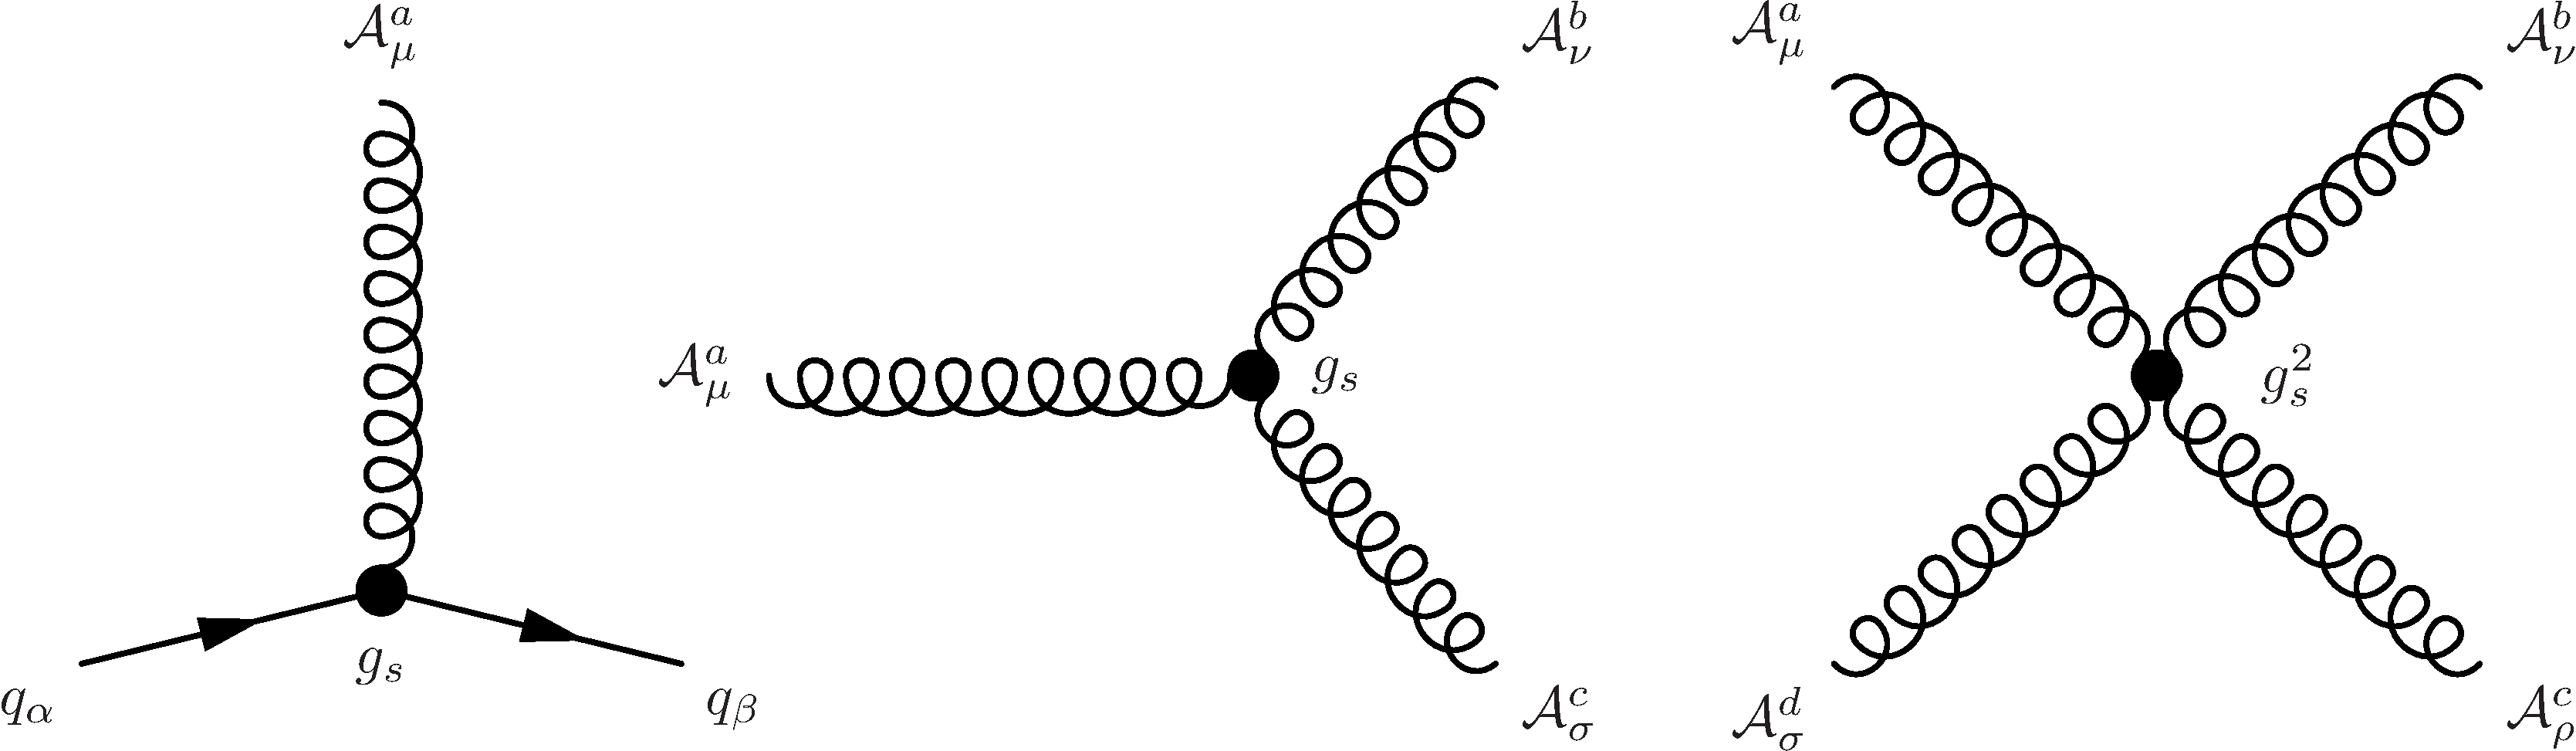
\includegraphics[width=0.79\textwidth]{figures/theory/QCD_vtx.pdf}
\caption{The QCD interaction vertices: Quark interaction with the gluon field (left), and three- (middle) and four-gluon (right) self-interaction vertices.}
\label{fig:theory:qcdint}
\end{figure}
These self-interactions have severe consequences: any bare color charge, like a quark, will be surrounded by a sea of virtual gluons and quarks that share the same color. When probing the quark color at higher and higher energies, corresponding to shorter and shorter distances, the color charge decreases until only the bare charge is visible. There, the quarks are essentially free and can be observed as distinguishable particles. This property is referred to as \emph{asymptotic freedom}. For the same reasons, when going further and further away from a bare color charge, the sea of charges surrounding it makes the observed charge increase. That results in a strong attractive force between color charges at large distances, where the potential energy between the two grows linearly with the distance between them as
\begin{equation}
  V(r)=-\frac{4\alpha_s}{3r}+kr,
\end{equation} 
where $r$ is the distance between the quarks and $\alpha_s$ is the coupling strength of QCD.
%, describing how the observed charge between two quarks increases depending on the distance between them. 
When the distance between the quarks grows very large, this potential energy is enough to create real quark-antiquark pairs from the vacuum in order to reduce the potential energy, a process called \emph{fragmentation}. Whenever one tries to separate quarks form one another they will fragment, which consequently means that quarks are never observed on their own. Rather, they form colorless (uncharged under the color charge) bound states of mesons or baryons (collectively called hadrons), a property called \emph{color confinement}. The energy for which the confinement into hadrons occurs, also called \emph{hadronization}, is defined through experimental measurement and found to be $\Lambda_{QCD}=100-500 \MeV$ (around the mass of the lightest hadrons). The effective charge between the quarks, $\alpha_S$, changes as a function of energy as
 \begin{equation}
   \alpha_S(Q)=-\frac{6\pi}{33-2n_f}\ln(Q/\Lambda_{QCD})
 \end{equation}
where $Q$ is the energy of the probe used to measure the charge and $n_f$ is the number of quark flavors (u, d, c, s, b, t) at that energy. $\alpha_S$ is around 0.1 for energies between 100-1000 \GeV.

\subsection{The electroweak sector}
\label{sec:theory:ew}
The electromagnetic and weak interactions arise from the breaking of $SU (2)_L \otimes U(1)_Y$ symmetry. While the unification of the electromagnetic and weak force is obtained under the $SU (2)_L \otimes U(1)_Y$ group, the predicted gauge bosons of such a group are not observed in nature: three charged massless vector bosons and one neutral massless boson. Rather, the $\PW^{\pm}$, $\PZ^{0}$ and the photon arise from the spontaneous symmetry breaking of $SU (2)_L \otimes U(1)_Y$ to $U(1)_{EM}$. This happens due to the \emph{Higgs mechanism}, and exactly how this occurs will be the topic of Section~\ref{sec:theory:higgs}.\par
The symmetry under $SU (2)_L$ is called weak left-handed isospin $L$, and the symmetry under $U(1)_Y$ is the weak hypercharge $Y$. The name "left-handed" arise from the fact that \emph{parity} is violated in the electroweak interactions. All the fundamental fermions have a \emph{chirality}, defined as the projection of the particles spin along its direction of motion. Weak interactions are only observed for fermions of left-handed chirality (vector minus axial coupling, V-A). While the left-handed fermion fields are in the simplest doublet representation of $SU(2)$ with weak isospin $I=1/2$, the fermions of right-handed chirality are therefore in the singlet representation with weak isospin $I=0$, meaning they do not interact with the gauge bosons of $SU (2)_L$. The chirality of any fermion $\Psi$ can be defined through the operator $\gamma^5$, the product of the four Dirac matrices~\cite{Pauli:1936gd} $\gamma^5=i\gamma^1\gamma^2\gamma^3\gamma^4$. Any fermion field can be projected into its chiral components $\Psi_L$ or $\Psi_R$ through the projection operation
\begin{equation}
  \Psi_L = \frac{1-\gamma^5}{2} \quad \textrm{and} \quad \Psi_R = \frac{1+\gamma^5}{2}.
  \end{equation}
The gauge field tensor of the group of $SU (2)_L$ symmetry is $W_{\mu\nu}^a$, where $a$ runs over the 3 generators of the group. The conserved charge associated with the group is the \emph{third} component of weak isospin $I_3$, and all weak interactions must preserve $I_3$. The generators of the group are defined as $T_i=\frac{\sigma_i}{2}$, where $\sigma_i$ are the Pauli matrices~\cite{inbook}. As for $SU (3)_C$, the group is non-abelian and the generators follow the commutation relation $[\sigma_i/2,\sigma_j/2]=i \epsilon_{ijk} \sigma_k/2$, where $\epsilon_{ijk}$ is the Levi-Civita permutation symbol~\cite{Duplij2004}. This in turn implies self-interactions between the gauge bosons of the group.\par
The latter group, $U(1)_Y$ of weak hypercharge $Y$, is abelian and hence display no self-interaction. The gauge field tensor $B_{\mu\nu}^a$ interacts with both left- and right-handed fermion fields. Similar to the case for QCD, a local gauge transformation of $SU (2)_L \otimes U(1)_Y$ requires the addition of additional terms in the derivate in order to keep the Lagrangian invariant. The partial derivative $\partial_{\mu}$ is replaced by the covariant derivatives
\begin{align}
  \label{eq:theory:ewcov}
  D_\mu \Psi_L &=(\partial_{\mu} + ig_2 T_a W_{\mu}^a + ig_1 \frac{Y}{2} B_{\mu}^a)\Psi_L\\
  D_\mu \Psi_R &=(\partial_{\mu} + ig_1 \frac{Y}{2} B_{\mu}^a)\Psi_R.
\end{align}
After the substitution, the electroweak Lagrangian can be written as a sum of four terms:
\begin{equation}
  \label{eq:theory:ewl}
   \mathcal{L}_{EW} = \mathcal{L}_{gauge}+\mathcal{L}_{f}+\mathcal{L}_{Yukawa}+\mathcal{L}_{\phi}.
\end{equation}
\par The first term, $\mathcal{L}_{gauge}$, represent the kinetic field tensor and is
\begin{equation}
  \label{eq:theory:gauge}
   \mathcal{L}_{gauge} = -\frac{1}{4}W_{a}^{\mu\nu}W^{a}_{\mu\nu} - \frac{1}{4}{\cal B}^{\mu\nu}{\cal B}_{\mu\nu}
\end{equation}
where the gauge field tensors are
\begin{align}
W_{\mu\nu}^a &=\partial_{\mu} W_{\nu}^a-\partial_{\nu} W_{\mu}^a-g_2\epsilon^{ijk}W^{j}_{\mu}W^{k}_{\nu} \quad \textrm{, with   } i=1-3\\
B_{\mu\nu} &=\partial_{\mu} B_{\nu}-\partial_{\nu} B_{\mu}.
\end{align}
The non-abelian nature of $SU (2)_L$ leads to trilinear and quadrilinear couplings between the photon and vector bosons as illustrated in Figure~\ref{fig:theory:weakint}.
\begin{figure}[h!]
\centering
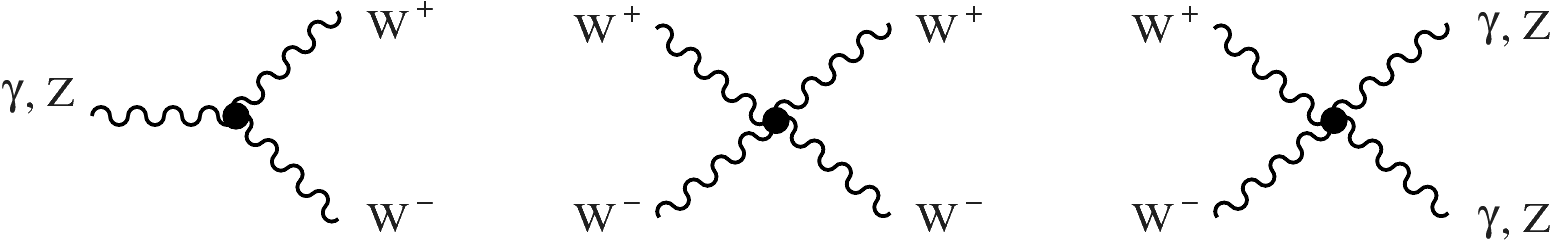
\includegraphics[width=0.99\textwidth]{figures/theory/weak_selfinteraction.png}
\caption{The electroweak self-interaction vertices: trilinear (left), and quadri-linear (middle and right) vertices.}
\label{fig:theory:weakint}
\end{figure}
\par The second term describe the boson fields coupling to fermions and is
\begin{equation}
  \label{eq:theory:gauge}
   \mathcal{L}_{f} = \bar{Q}_ii\lambda^{\mu}D_{\mu} Q_i + \bar{u}_i^ci\lambda^{\mu}D_{\mu} u_i^c
                   + \bar{d}_i^ci\lambda^{\mu}D_{\mu} d_i^c + \bar{L}_ii\lambda^{\mu}D_{\mu} L_i +  
                     \bar{e}_i^ci\lambda^{\mu}D_{\mu} e^c_i,
\end{equation}
where we have expressed each term using the particle multiplets in Equation~\ref{eq:theory:multiplets} and the subscript $i$ runs over the three fermion generations. They all interact differently under $SU(2)_L \times U(1)_Y$ due to their different charges.\newline
Up until now we have considered the Lagrangian before spontaneous symmetry breaking, where we have three charged massless bosons and one massless neutral boson, a constellation we know to be wrong from observations. When I have referred to interaction vertices, I have loosely referred to W, Z and $\gamma$ vertices without explicitly defining them. We will show in Section~\ref{sec:theory:higgs} that, due to spontaneous symmetry breaking, the charged gauge boson fields $\PW^{\pm}$ in reality are linear combinations of $W_{\mu}^1$ and $W_{\mu}^2$ given as
\begin{equation}
\PW^{\pm} = \frac{1}{\sqrt{2}}(W_{\mu}^1 \mp iW_{\mu}^2).
\end{equation}
These are responsible for \emph{charged current interactions}, which turn up-type fermions into their corresponding down-type fermions within the same generation, and vice-versa. The electrically neutral Z boson and the photon fields are expressed in terms of $W_{\mu}^3$ and $B_{\mu}$ through the weak mixing angle~\cite{Weinberg:1979pi} as
\begin{equation}
\begin{pmatrix} \gamma \\ \PZ^0 \end{pmatrix}
  = \begin{pmatrix} \cos \theta_W & \sin \theta_W \\
                   -\sin \theta_W & \cos \theta_W \end{pmatrix}
  \begin{pmatrix} B \\ W^3 \end{pmatrix}                   
\end{equation}
where $\theta_W$ can be expressed through the $SU (2)_L$ and $U(1)_Y$ couplings $g_1$ and $g_2$ as
\begin{equation}
     \cos \theta_W = \frac{g_1}{g^2_1+g^2_2}  \quad \textrm{ and } \quad \sin \theta_W = \frac{g_2}{g^2_1+g^2_2}.        
\end{equation}
The electric charge is defined through weak isospin and hypercharge, and is
\begin{equation}
  Q = I_3 + \frac{Y}{2}.
  \end{equation}
A few of the fermion-boson vertices are shown in Figure~\ref{fig:theory:weakfermionint}.\par
  \begin{figure}[h!]
  \centering
  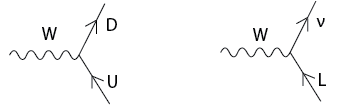
\includegraphics[width=0.45\textwidth]{figures/theory/ew_ch.png}\\
  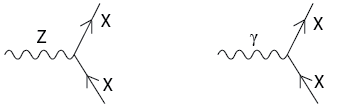
\includegraphics[width=0.45\textwidth]{figures/theory/ew_neu.png}
  \caption{The electroweak fermion interaction vertices. Top: Charged current interaction vertex connecting a charged vector boson $\PW^{\pm}$ to quarks (left) and leptons (right). Bottom: Neutral current interactions between the neutral $\PZ^0$ boson and any fermion (left), and between a $\gamma$ and electrically charged fermions.}
  \label{fig:theory:weakfermionint}
  \end{figure}
The last two terms, $\mathcal{L}_{Yukawa}$ and $\mathcal{L}_{\phi}$, are related to the Higgs boson and represent couplings to the Higgs field: the Yukawa interaction term which generates masses for the fermions due to the non-zero Higgs vacuum expectation value, and the Higgs bosons interactions with itself and with the gauge bosons. Introduced as an extension to the original Standard Model, the Higgs sector is one of the greatest accomplishments of particle physics in the 20th century and one of the reasons why the LHC was built. How it arises is what we will turn to next.

\subsection{The Higgs sector}
\label{sec:theory:higgs}
The problem of having massless gauge bosons under $SU(2)_L \times U(1)_Y$, while observing massive W and Z bosons, was independently solved by three different groups and has become known as the Englert–Brout-Higgs–Guralnik–Hagen–Kibble mechanism of spontaneous symmetry breaking~\cite{PhysRevLett.13.321,PhysRevLett.13.508,PhysRevLett.13.585}, an accomplishment for which Peter Higgs and Francois Englert shared the 2013 Nobel Prize.\newline
It began with the realization that the breaking of a local gauge symmetry could give rise to a final mass for the gauge boson involved. This was first discovered in association with superconductivity, where it was found that when a normal metal becomes superconducting the photon field inside the superconductor would acquire a finite mass~\cite{PhysRev.110.827}.

\subsubsection{Spontaneous breaking of a global gauge symmetry}
In order to achieve spontaneous symmetry breaking, Jeffrey Goldstone~\cite{Goldstone:1961eq} suggested introducing a massive complex scalar field $\phi$ with quantum numbers of the vacuum and then give the field a vacuum expectation value. The field
\begin{equation}
\phi = \frac{1}{\sqrt{2}}(\phi_1+i\phi_2)  
\end{equation}
would have a Lagrangian of the form
\begin{equation}
\mathcal{L} = \partial^{\mu}\bar{\phi}\partial_{\mu}\phi-\mu_0^2\bar{\phi}\phi-\frac{\lambda_0}{6}\bar{\phi}\phi^2,
\end{equation}
where $\lambda_0$ is the coupling constant and $\mu_0$ is the mass. The Lagrangian is invariant under $U(1)$, though in this case under a global symmetry and not a local one. If one takes $\mu_0^2$ to be negative, the potential will get a minima along a circle of radius $v$ such that
\begin{equation}
  \phi_1^2+\phi_2^2 = v^2 \quad \textrm{and}\quad v^2=\frac{\mu_0^2}{\lambda_0}
\end{equation}
and take the form of a "Mexican Hat" as shown in Figure~\ref{fig:theory:higgspot}. 
  \begin{figure}[h!]
  \centering
  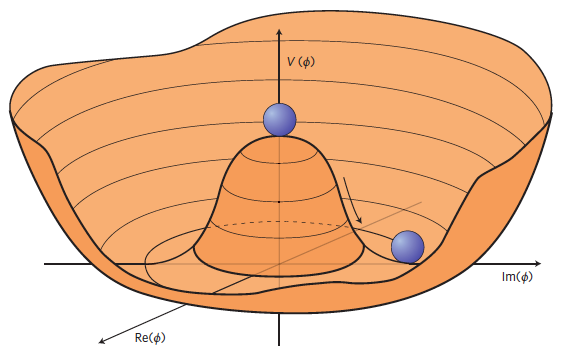
\includegraphics[width=0.49\textwidth]{figures/theory/higgspotential.png}
  \caption{The potential $V(\phi)$ for a complex scalar field with $\mu_0^2<0$~\cite{Ellis:1638469}.}
  \label{fig:theory:higgspot}
  \end{figure}
The variable $v$ is referred to as the vacuum expectation value (VEV). The lowest value of the Hamiltonian is now at $\phi=v$ rather than at $\phi=0$. Goldstone then translated the field to a minimum energy position $\phi'=\phi+v$ and gave the field a vacuum expectation value, effectively breaking the symmetry between the two field components, but keeping the Lagrangian invariant.
This complex field can be expanded around the ground state in terms of two real fields $\eta$ and $\epsilon$ that represent deviations from the minimum:
\begin{equation}
\phi(x) = \frac{1}{\sqrt{2}}*(v+\eta(x)+i\epsilon(x))
\end{equation}
 The Lagrangian then becomes
\begin{equation}
\mathcal{L} = \frac{1}{2}(\partial_{\mu}\epsilon)^2 + \frac{1}{2}(\partial_{\mu}\eta)^2+\mu_0^2\eta^2 + \textrm{ additional terms}.
\end{equation}
The third term has the form of a mass term for the scalar $\eta$ field. However, the $\epsilon$ field has no mass term meaning that the theory contains a massless scalar, referred to as a \emph{Goldstone boson}. This is expressed through \emph{Goldstones theorem}, which states that whenever a continuous symmetry of a physical system is spontaneously broken, massless scalars will occur. Rather than providing a mass term for the vector bosons, the theory acquired one massive scalar and one massless scalar not observed in nature, requiring the gauge theory of weak interactions to look for solutions elsewhere.

\subsubsection{The Higgs mechanism}
The solution to the problem came a few years later, in 1964, when spontaneous symmetry breaking of a \emph{local} gauge symmetry was studied gather than a global. For a $U(1)$ symmetry, this requires the Lagrangian to be invariant under $\phi \rightarrow e^{i\theta(x)}\phi$ with the derivative replacement
\begin{equation}
D_{\mu}=\partial_{\mu}-ie A_{\mu}.
\end{equation}
After translating the field $\phi$ to its true ground state and writing out the Lagrangian
\begin{equation}
  \label{eq:theory:higgsL}
\mathcal{L} = \frac{1}{2}(\partial_{\mu}\epsilon)^2 + \frac{1}{2}(\partial_{\mu}\eta)^2-v^2\lambda \eta^2+\frac{1}{2}v^2 e^2 A_{\mu} A^{\mu}-ev A_{\mu}\partial^{\mu}\epsilon-\frac{1}{4}F_{a}^{\mu\nu}F^{a}_{\mu\nu}
\end{equation}
we see that the particle spectrum now contains a massless Goldstone boson $\epsilon$, a massive scalar $\eta$ and, finally, a massive vector $A_{\mu}$ with $m_A=ev$. Despite the success of having dynamically created the mass for the gauge field, one had to tackle the problem of the massless scalar. The solution was found through the realization that one of the fields were unphysical; by giving mass to the vector $A_{\mu}$, the polarization degrees of freedom had increased from 2 to 3 through adding a longitudinal polarization. However, this should not be possible when simply translating field variables. It was found that through a simple gauge transformation with a different set of fields
\begin{equation}
A_{\mu} \rightarrow A_{\mu}+\frac{1}{ev}\partial_{\mu}\theta,
\end{equation}
the Goldstone boson would disappear and turn into the longitudinal polarization of the massive gauge boson and the theory was left with one massive vector gauge boson $A_{\mu}$ and another massive scalar $h$. This is what is referred to as the \emph{Higgs mechanism}.

\subsubsection{The Weinberg-Salam Model}
The final step is to formulate the Higgs mechanism such that the vector bosons $\PW^{\pm}$ and $\PZ^{0}$ become massive, while the photon remains massless. To do so Sheldon Glashow, Abdus Salam, and Steven Weinberg (all awarded the 1979 Nobel Prize for electroweak unification), added a gauge invariant term to the electroweak Lagrangian of the following form:
 \begin{align}
   \label{eq:theory:higgsmass}
  \mathcal{L}_{Higgs}= \big|(i\partial_{\mu} - g_2 T_a W_{\mu}^a -vg_1 \frac{Y}{2} B_{\mu}^a) \phi\big| ^2-V(\phi)
 \end{align}
The $\phi_i$ has to belong to $SU(2) \times U(1)$ multiplets, and the simplest constellation corresponds to four fields in an isospin doublet of weak hypercharge $Y=1$:
\begin{equation}
\phi =  \begin{pmatrix} \phi^{+} \\ \phi^{0} \end{pmatrix}= \begin{pmatrix} \frac{\phi_1+i\phi_2}{\sqrt{2}} \\ \frac{\phi_3+i\phi_4}{\sqrt{2}}\end{pmatrix}.
\end{equation}
To generate the necessary masses, the Higgs potential from the previous section is used, with a vacuum expectation value of
\begin{equation}
\phi_0 = \frac{1}{\sqrt{2}}  \begin{pmatrix} 0 \\ v \end{pmatrix}.
\end{equation}
This specific choice of charges, VEV and fields insure that the $U(1)_{em}$ symmetry with $Q=T^3+\frac{Y}{2}$ remains unbroken, keeping the photon massless. The three others break the symmetry and become massive gauge bosons: the $\PW^{+}$, $\PW^{-}$ and $\PZ^{0}$. The mass terms for the gauge bosons finally become
\begin{equation}
M_W=\frac{1}{2}vg_1 \quad \textrm{and} \quad M_Z =\frac{1}{2}v\sqrt{g_1^2+g_2^2},
\end{equation}
with the Weinberg angle $\theta_W$ defined as
\begin{equation}
\textrm{with}\quad\frac{M_W}{M_Z}=\cos \theta_W.
\end{equation}
As mentioned in Section~\ref{sec:theory:ew}, the fermions also get their masses through interacting with the Higgs field, corresponding to the $\mathcal{L}_{Yukawa}$ term in the electroweak Lagrangian. This is done the same way as for the bosons: an additional $SU(2) \times U(1)$ invariant term for each generation is added, for instance for the electron
\begin{equation}
  -G_e \bigg[ \begin{pmatrix} \bar{\nu}_e & \bar{e}\end{pmatrix}_L   \begin{pmatrix} \phi^{+} \\ \phi^{0} \end{pmatrix} e^R +
  \bar{e}_R  \begin{pmatrix} \phi^{-} & \bar{\phi}^{0} \end{pmatrix}  \begin{pmatrix} \nu_e \\ e\end{pmatrix}_L  \bigg],
  \end{equation}
where $G_E$ is the electron coupling. We then spontaneously break the symmetry with
\begin{equation}
\phi = \frac{1}{\sqrt{2}}  \begin{pmatrix} 0 \\ v+h(x) \end{pmatrix},
\end{equation}
 where the neutral Higgs field $h(x)$ is the only remnant of the Higgs doublet after spontaneous symmetry breaking. After substitution, the final Lagrangian for the electron mass becomes
 \begin{equation}
   \mathcal{L}_{Yukawa}^e=-\frac{G_e}{\sqrt{2}}v(\bar{e}_L e_R + \bar{e}_R e_L )(1+\frac{h}{v}).
\end{equation}
We can choose $G_e$ such that
\begin{equation}
  m_e=-\frac{G_e v}{\sqrt{2}}
  \end{equation}
and generate the electron mass as
\begin{equation}
  \mathcal{L}_{Yukawa}^e=-m_e \bar{e}e-\frac{m_e}{v} \bar{e}eh.
\end{equation}  
In summary, all the fermion masses are generated through the interaction of the fermion fields with the Higgs field. From the equation above, we see that the fermion masses are not predicted from the theory as the coupling $G$ is arbitrary. The Standard Model therefore cannot provide an explanation for the difference in hierarchy between the couplings. We also see that the Lagrangian contains an interaction term coupling the Higgs scalar to the fermions and that this term depends on the mass of the fermion. The Higgs boson therefore couples more strongly to heavy fermions than to lighter ones.
     
\clearpage
\chapter{Beyond Standard Model Physics}
\section{Shortcomings of the Standard Model}
Despite being an extremely successful and predictive theory, the Standard Model has its shortcomings. The most obvious one is its failure to successfully incorporate the gravitational force. Gravity is beautifully described in General Relativity as a classical theory: a force caused by the curvature of space-time in the presence of matter and energy. The theory does not utilize quantum fields and energy is not quantized.
The scales between the Standard Model, a quantum field theory, and General Relativity are completely different: space-time is curved on astronomical scales, where the force of gravity is measurable, while quantum field theories deal with things on the smallest possible scales, where variations in space-time are essentially invisible. Hence, to the Standard Model, space-time is approximately flat and gravity does not exist. In order to have an elegant unified theory of all the forces, attempts has been made to have a quantum field theory of the gravitational force by extending the Standard Model particle family to incorporate a particle to mediate the gravitational force called the \emph{graviton}, a massless gauge boson of spin-2. The problem is that gravity is universally attractive, meaning nothing "cancels" it. That leads to loop divergences that cannot be reabsorbed through renormalization and every effort of integrating gravity in the SM has thus far failed. 
%However, it has been shown that General Relativity is an inevitable consequence of the quantum mechanics of interacting gravitons, which has led to several proposals for extending the SM models to incorporate them.\newline
In addition to the difficulties of incorporating gravity into a quantum field theory framework, problems occur at small distances at which quantum gravitational effects would become apparent, the Planck scale. This can be represented by the Planck mass, the mass of the smallest possible black hole. When comparing the Planck mass to the masses of the electroweak bosons \PW and \PZ, we find that the Planck mass is $10^{16}$ times heavier than the electroweak bosons, such that there is a \emph{hierarchy} between the mass scales of gravity and the electroweak forces. The reason why this observed hierarchy occurs has to do with the Higgs vacuum expectation value (VEV): the Higgs field has a measured vacuum expectation value of 246 GeV and this is, as discussed in the section above, what gives the W and Z bosons their mass. However, when actually calculating the Higgs VEV and taking all loop corrections into account, it would receive corrections on the order of the Planck energy, yielding a Higgs boson mass $10^{16}$ times larger than observed. This is called the \emph{hierarchy problem}.
Quantum loop corrections of this magnitude only happen for scalar particles such as the Higgs boson. Fermions are protected from such divergences through their chiral structure, and gauge bosons are protected through gauge invariance. The question is then why the Higgs VEV, and consequently the Higgs, W and Z boson masses are so much smaller than the natural mass scale.\newline
Of course, it is possible that the Higgs boson mass just happens to be 125 \GeV due to some fine-tuned, large cancellations that keeps the mass from approaching the Planck mass, as is currently held by the Standard Model. However, this is neither very elegant nor very probable without a well-motivated reason why such a cancellation should occur. Rather, in order to resolve the problem of scales, theories Beyond the Standard Model (BSM) have been introduced. The theories that I will probe in this thesis are amongst those.\par
Two Beyond Standard Model theories will be considered in this thesis: Compositeness and extra dimensional theories.
Compositeness attacks the hierarchy problem by assuming that the Standard Model breaks down at an energy between the weak and Planck scales and that, around the \TeV scale, the Higgs boson no longer appears to be a single scalar particle but a composite state of two fermions. In the following, I will present the study of composite models in the context of the \emph{Heavy Vector Triplet formalism}, described in Section~\ref{sec:theory:hvt}. Warped extra dimensional theories on the other hand, attempt to solve the hierarchy problem by forcing gravity to be concentrated on another "brane" and letting its strength fall of exponentially through an extra dimension.

\section{Compositeness}
In composite Higgs models, the Higgs boson is assumed to be a bound state of fundamental constituents held together by some new strong force~\cite{Bellazzini:2014yua,Contino:2011np}. This removes the hierarchy problem since we no longer have an elementary scalar in the Standard Model, hence no loop corrections going to infinity. The compositeness of the Higgs boson becomes apparent at the energy scale $\Lambda$, where $\Lambda$ has to be at least 10 \TeV, since anything below that is ruled out by electroweak precision measurements.
The Higgs boson is assumed to be a pseudo-Goldstone boson of some approximate symmetry, where pseudo-Goldstone bosons are bosons with a tiny mass that approach zero in the limit of the symmetry becoming exact. The approximate symmetry is broken at the scale $f$, where $\Lambda=4\pi f$. Being a pseudo-Goldstone boson, the Higgs boson mass is protected from divergent quantum loop corrections up to the scale of compositeness and, above that scale, is no longer an elementary scalar.
The theory is based on the breaking of two parallel global symmetries $[SU(2)_1 \times U(1)_1]\times[SU(2)_2 \times U(1)_2]$, with Goldstone bosons becoming the longitudinal components of the three predicted gauge bosons of the symmetry group $\mathrm{W}^{\prime\pm}$ and $\PZpr$. These have masses of the order of the compositeness scale
\begin{equation}\label{eqn:LHvprimeMass}
M(\mathrm{W}^{\prime\pm}) \simeq M(\PZpr) = \frac{g}{\sin2\theta}f,
\end{equation}
\noindent where $\tan\theta = g_1/g_2$, the ratio of couplings of the $SU(2)$ groups. The predicted decay widths are roughly the same for \PZpr and \PWpr and are as follows:
\begin{equation}
\begin{aligned}
\Gamma(\mathrm{W}^{\prime\pm} \to \ell\nu, \PZpr \to \ell\ell) & = \frac{g^2\cot^2\theta}{96\pi}M\\
\Gamma(\mathrm{W}^{\prime\pm} \to \mathrm{q}\bar{\mathrm{q}}^\prime,\PZpr \to \qqbar) & = \frac{g^2\cot^2\theta}{32\pi}M\\
\Gamma(\mathrm{W}^{\prime\pm} \to \PW\PZ,\PZpr \to \PW\PW) & = \frac{g^2\cot^22\theta}{192\pi}M
\end{aligned} 
\end{equation}
Decays into fermions therefore dominate at $\cot\theta \geq 1/2$, whereas decays into bosons are enhanced for very low $\cot\theta$. These generic composite models can be studied with the Heavy Vector Triplet formalism.

\subsection{Heavy Vector Triplet formalism}
\label{sec:theory:hvt}
There are many BSM theories that predict the presence of spin-1 particles with masses at the \TeV scale, each with their own list of model parameters. In most cases, however, when looking for such new particles, experiments are not sensitive to the specifics of the model but only the masses and couplings of the resonances. We can therefore start from a \emph{simplified model} that describes the dynamics of the new spin-1 vector through a simple phenomenological Lagrangian that only retains couplings and mass. In the Heavy Vector Triplet formalism~\cite{Pappadopulo:2014qza}, a real vector $V_{\mu}^a$, where $r$ runs from 1 to 3, is introduced in the adjoint representation of $SU(2)L$ and represents one charged
and one neutral heavy spin-one particle with charge eigenstates
\begin{equation}\label{eqn:HVT_1}
V^\pm_\mu = \frac{V^1_\mu \mp iV^2_\mu}{\sqrt{2}} \qquad \textrm{and}\qquad V^0_\mu = V^3_\mu.
\end{equation}
The simplified Lagrangian governing the dynamics is given as
\begin{equation}
\begin{split}
\mathcal{L}_V = & -\frac{1}{4}\mathcal{D}_{[\mu}V^a_{\nu]}\mathcal{D}^{[\mu}V^{\nu]a} + \frac{m^2_V}{2}V^a_\mu V^{\mu a}\\
 & + ig_Vc_HV^a_\mu H^\dag\tau^a\overleftrightarrow{\mathcal{D}}^\mu H + \frac{g^2}{g_V}c_FV^a_\mu J^{\mu a}_F\\
 & + \mbox{additional terms.}
 \end{split}
\end{equation}
The first line describes the kinematic and mass terms of the vector $V$, and the second line, which is of most interest to us, describes the coupling to the Higgs boson current and the left-handed fermionic currents.
In the coupling to the Higgs current, the coefficient $c_H$ leads to vertices involving the Higgs field and the Goldstone bosons, representing the longitudinally polarized SM vector bosons, \PW and \PZ.
This term therefore governs the decay modes of the vector $V$ into electroweak bosons, the decay mode of interest for this thesis. The second coupling term describes the interaction with leptons and quarks and is governed by the parameter $c_F$. A formalism is adopted where the interactions are weighted with a coupling $g_V$ and $g^2/g_V$, where $g$ is the gauge coupling of the group and $g_V$ represents the "typical strength" of the vector interactions. Another interesting feature of the theory is that, after electroweak symmetry breaking provides the heavy vector with its mass, the charged and neutral vectors are found to be mass degenerate and expected to have similar production and decay rates.\newline
After having defined the generic framework, explicit models with fixed values of $c_H$ and $c_f$ can be studied, where only the resonance mass $m_V$ and coupling $g_V$ are left as free parameters.
In this thesis, we probe two benchmark models called HVT model A and HVT model B, as introduced in~\cite{Pappadopulo:2014qza}. The reason why these two models are interesting is that the first probes rather weakly coupled extensions of the SM, and the latter, strongly coupled scenarios. That implies very different sizes of $g_V$, where values of $g_V = 1$ for model A and $g_V = 3$ for model B are used in~\cite{Pappadopulo:2014qza}. For these values of $g_V$, model A predicts a comparable branching fraction for decays into bosons and fermions, the decay into fermions only enhanced by a factor of 2, while for model B, the dominant branching fraction is to dibosons with decays into fermions severely suppressed. The branching fraction for the different decay modes of HVT model A and B, are shown in Figure~\ref{fig:theory:hvtBR}. For obvious reasons, model B is of most interest for the searches presented here.
\begin{figure}[h!]
\centering
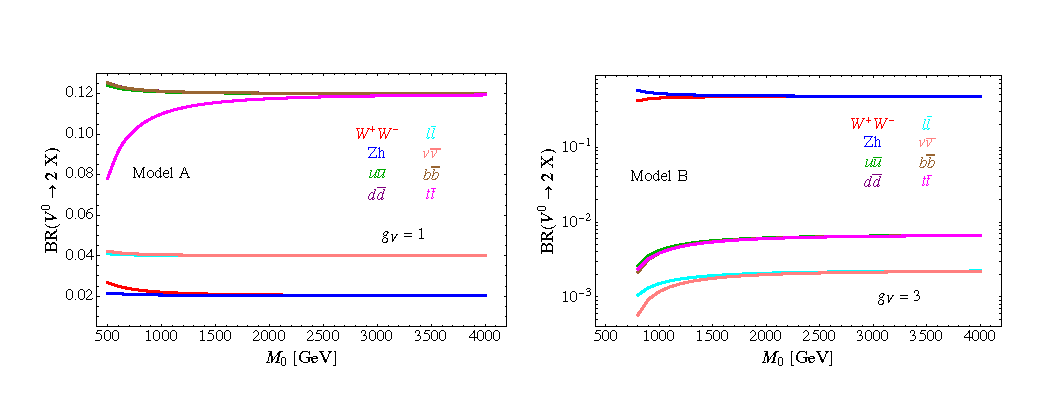
\includegraphics[width=0.99\textwidth]{figures/theory/hvtmodels.pdf}
\caption{Predicted branching fractions of a \PZpr for two explicit HVT models: Model  $\mathrm{A}_{g_V=1}$ (left) and model $\mathrm{B}_{g_V=3}$ (right)~\cite{Pappadopulo:2014qza}.}
\label{fig:theory:hvtBR}
\end{figure}
\clearpage

\section{Warped extra dimensions}
\label{sec:theory:wed}
Extra dimensional theories also offer solutions to the hierarchy problem. This thesis focuses on Randall-Sundrum (RS) warped extra dimensional scenarios~\cite{PhysRevLett.83.3370}. In RS models, a new curved spatial dimension $y$ is proposed, leading to a 5-dimensional space-time bounded by two (3+1)-dimensional planes, or \emph{branes}: the UV/Planck and the IR/TeV brane. The new metric now depends on the radius $r$ and the curvature factor $k$ of the new extra dimension
\begin{equation}
  ds^2=e^{-2ky}\eta_{\mu\nu}dx^{\mu}dx^{\nu}+dy^2; 0 < y < \pi R
\end{equation}
Gravity is concentrated and relatively strong at the Planck brane at $y=0$, which is separated from us by the fifth dimension. Our observed four-dimensional reality and the Standard Model particles reside at the \TeV brane, at $y=\pi R$. Only gravity, transmitted through gravitons, is allowed to propagate through the warped 5D space-time (the "bulk") and is not confined to either brane. Figure~\ref{fig:theory:rs1} illustrates how the branes and the bulk are connected.
\begin{figure}[h!]
\centering
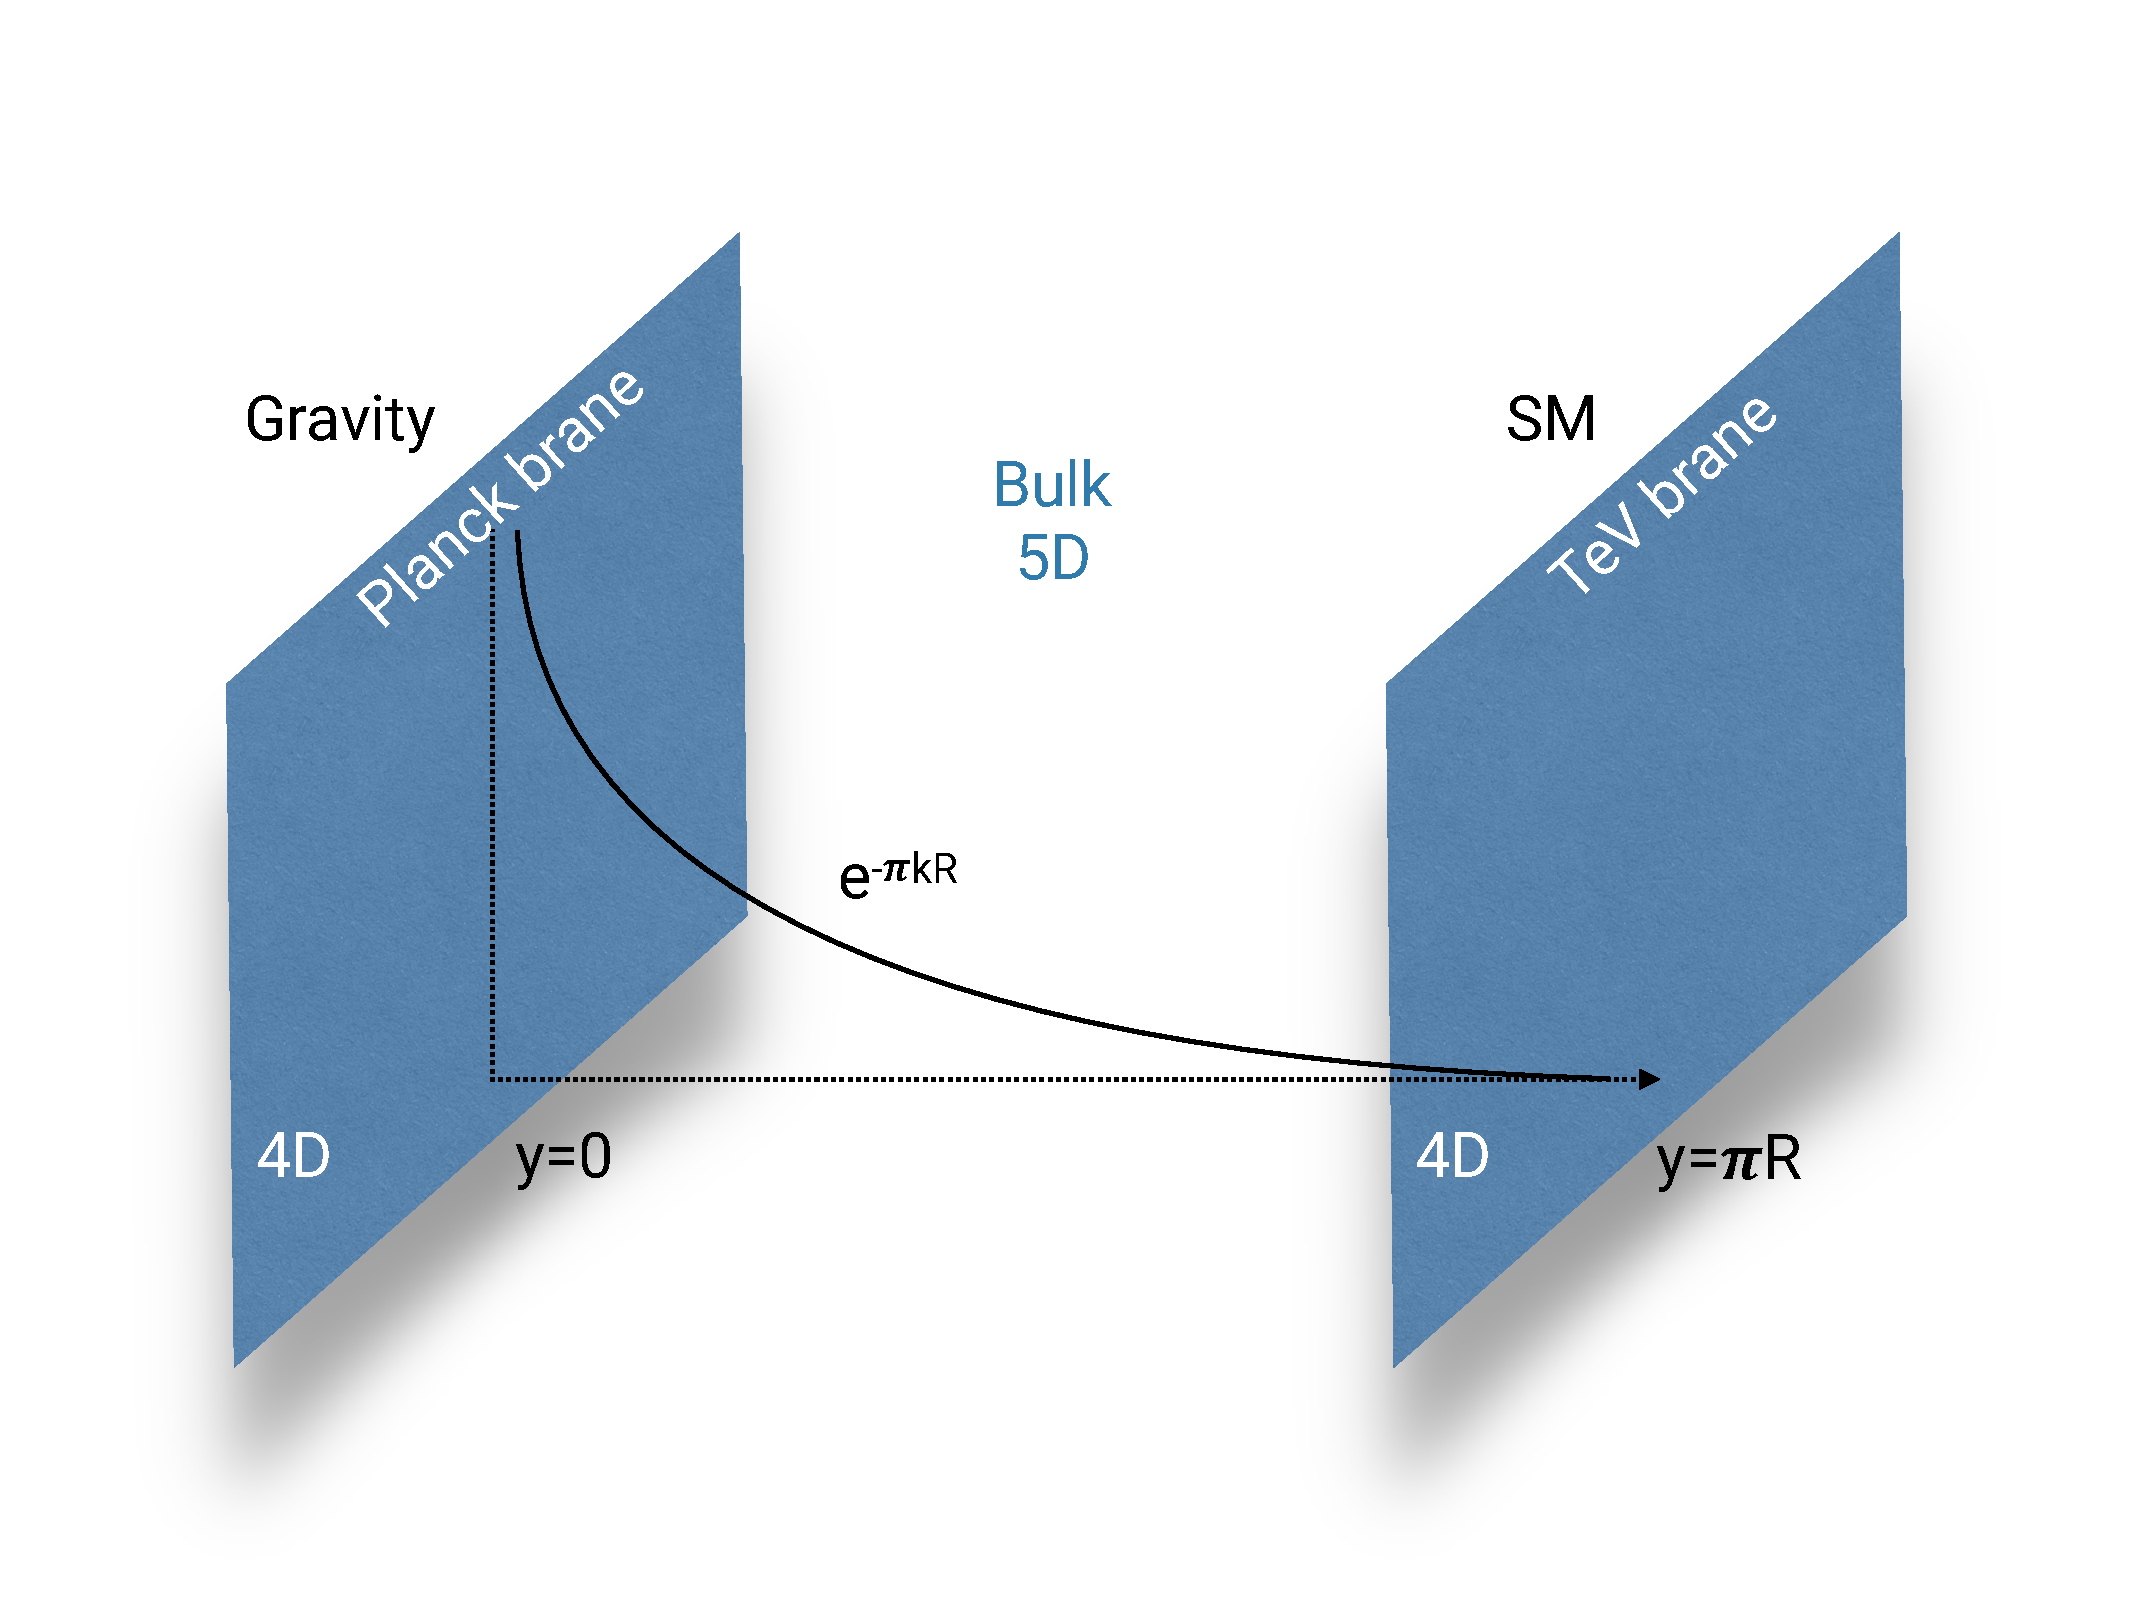
\includegraphics[width=0.49\textwidth]{figures/theory/rs1.pdf}
\caption{The RS model predicts an extra dimension where a 5D space-time stretches between two 4D branes: the Planck brane where gravity is concentrated, and the TeV brane where the SM particles are confined.}
\label{fig:theory:rs1}
\end{figure}
 Due to the warping, the Planck mass on the Planck brane gets reduced by a factor of $e^{-\pi kR}$ at the TeV brane, thereby solving the hierarchy problem. The Planck mass on the \TeV brane, which depends on the geometry of the extra dimension, becomes
\begin{equation}
  \bar{M}_{Pl}^2=V_1M_*^3,
  \end{equation} 
where $V_1$ is the volume of the 1 dimensional added warped dimension and $M_*^3$ is the 5D Planck mass.
One distinct prediction of the model, and a way in which we can test its validity, is the prediction of a tower of \TeV-scale excitations with spin-2, so called Kaluza-Klein states, that could be observed in high energy experiments. \newline
In this thesis, we are more interested in an alternative to the original RS model called the "bulk" scenario~\cite{PhysRevD.76.036006,Fitzpatrick:2007qr}. In this case, the Standard Model particles, besides the Higgs boson, are also allowed to propagate in the bulk. The light 1st and 2nd generation fermions are localized near the Planck brane, yielding small couplings to the Higgs boson that still resides at the \TeV brane, explaining their small masses. Similarly, the top quark is now located near the \TeV brane, resulting in a stronger Yukawa coupling to the Higgs boson. In addition, with the gravitons located near the \TeV brane and the fermions now residing near the Planck brane, the graviton coupling to fermions is strongly suppressed. SM gluons have a flat distribution throughout the bulk, making gluon-gluon production the dominant production channel of gravitons. Due to the weak vector bosons absorbing the Higgs degree of freedom in spontaneous symmetry breaking, their wave-functions fall of steeply near the \TeV brane, resulting in a coupling to the gravitons similar to that of the Higgs and the top. The only free parameters of the theory is the mass of the lightest KK graviton and the ratio $\tilde{k} = \frac{k}{\bar{M}_{Pl}}$, which controls the widths of the new resonances. The branching ratios of the Bulk Graviton is shown in Figure~\ref{fig:theory:bulk}.
\begin{figure}[h!]
\centering
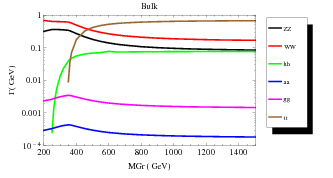
\includegraphics[width=0.49\textwidth]{figures/theory/BulkGravitonBR_tuomas.png}
\caption{Predicted branching fractions for a Bulk Graviton as a function of its mass.}
\label{fig:theory:bulk}
\end{figure}



% CMS
\chapter{Experimental setup}
\label{ch:CMS}
\section{The Large Hadron Collider}
In March 1984, the European Organization for Nuclear Research CERN) and the European Committee for Future Accelerators (ECFA) 
held a workshop in Lausanne entitled "Large Hadron Collider in the LEP Tunnel". 
This is history's first written mention of the Large Hadron Collider (LHC) and the topic under discussion 
was exactly how and where to build a new type of high-energy collider, capable of bringing hadrons
to collide rather than leptons.
The LHC would be housed in a tunnel which, at the time, was under excavation to host the Large Electron-Positron Collider (LEP) designed to collide leptons with center-of-mass-energies up to around 200 GeV.
LEP was a circular collider with a circumference of 27 km and the tunnel hosting it was located roughly 100 meters underground on the border between France and Switzerland, at the outskirts of Geneva. 
The justification for building a machine like the LHC, was that once LEP got to maximum reach, a new and more powerful collider would be needed in its place in order to probe higher energies.
While collisions of electrons with positrons provided exceptionally clean and precise measurements due to them being point particles,
 their lightness prevent them from being accelerated to higher energies. Collisions of hadrons, however, would allow for center-of-mass energies two orders of magnitude higher than that of LEP. Therefore, after running a while at two times the W mass (160 GeV) and reaching a maximum center-of-mass energy of 209 GeV, LEP was dismantled in 2000 in order to make room for the LHC.
 
The Large Hadron Collider started up in September 2008 and, while having the same 27-kilometer radius as the LEP collider, is capable of accelerating protons up to a center-of-mass energy of around 14 TeV, 70 times that of LEP. The accelerator consists of two oppositely going proton beams, isolated from each other and under ultrahigh vacuum, which are accelerated up to speeds close to that of the speed of light through radio frequency (RF) cavities, before being brought to collide at four different interaction points along the ring.
These four collision points correspond to the location of the four LHC particle detectors; ATLAS, CMS, LHCb and ALICE.
While ATLAS and CMS are general-purpose detectors built in order to study a large range of different physics processes, 
LHCb and ALICE are built for dedicated purposes; LHCb for b-physics processes and ALICE for heavy ion collision.
A protons journey from gas to one of the LHC collision points is as follows: First, hydrogen nuclei are extracted from a small tank of compressed hydrogen gas and stripped of their electrons. The remaining protons are then
injected into the LINAC2, a linear accelerator responsible for increasing the proton energy to about 50 MeV through RF cavities that push charged particles forward by switching from positive to negative electric fields. LINAC2 additionally divides the constant stream of particles into equally spaced "bunches" by careful tuning of the frequency of the field switch.
The accelerated protons are then injected into the Proton Synchrotron Booster (PSB), where their energy is increased thirty folds more, to an energy of roughly 1.4 GeV. The two final acceleration stages before the protons reach the LHC ring are the Proton Synchrotron and Super Proton Synchrotron, eventually leaving the protons with a total energy of 450 GeV. The protons are now ready for the final stage of their travel and are injected into the two beam pipes of the LHC in oppositely going direction. They are injected in trains of 144 bunches each ( with an order of $10^{11}$ protons per bunch), where each bunch is roughly 7.5 meters apart (or 25 ns). There are some larger beam gaps present in each beam in order to give the beam dump and injection kickers sufficient time to reach full voltage, where the largest one, the beam abort gap,  is roughly 3 ms or 900 m long. The ring is filled with proton bunches until these are equally distributed throughout the two rings, a process taking roughly 4 minutes. This is called a "fill". Here, the protons are accelerated to their maximum energy of 6.5 TeV, a process taking roughly 20 minutes, through eight RF cavities. These RF cavities are also responsible of keeping the proton bunches tightly bunched, ensuring maximum luminosity at the four collision points. A complete sketch of the CERN accelerator complex is shown in Figure~\ref{fig:cms:LHC}.

\begin{figure}[h] 
    \centering
    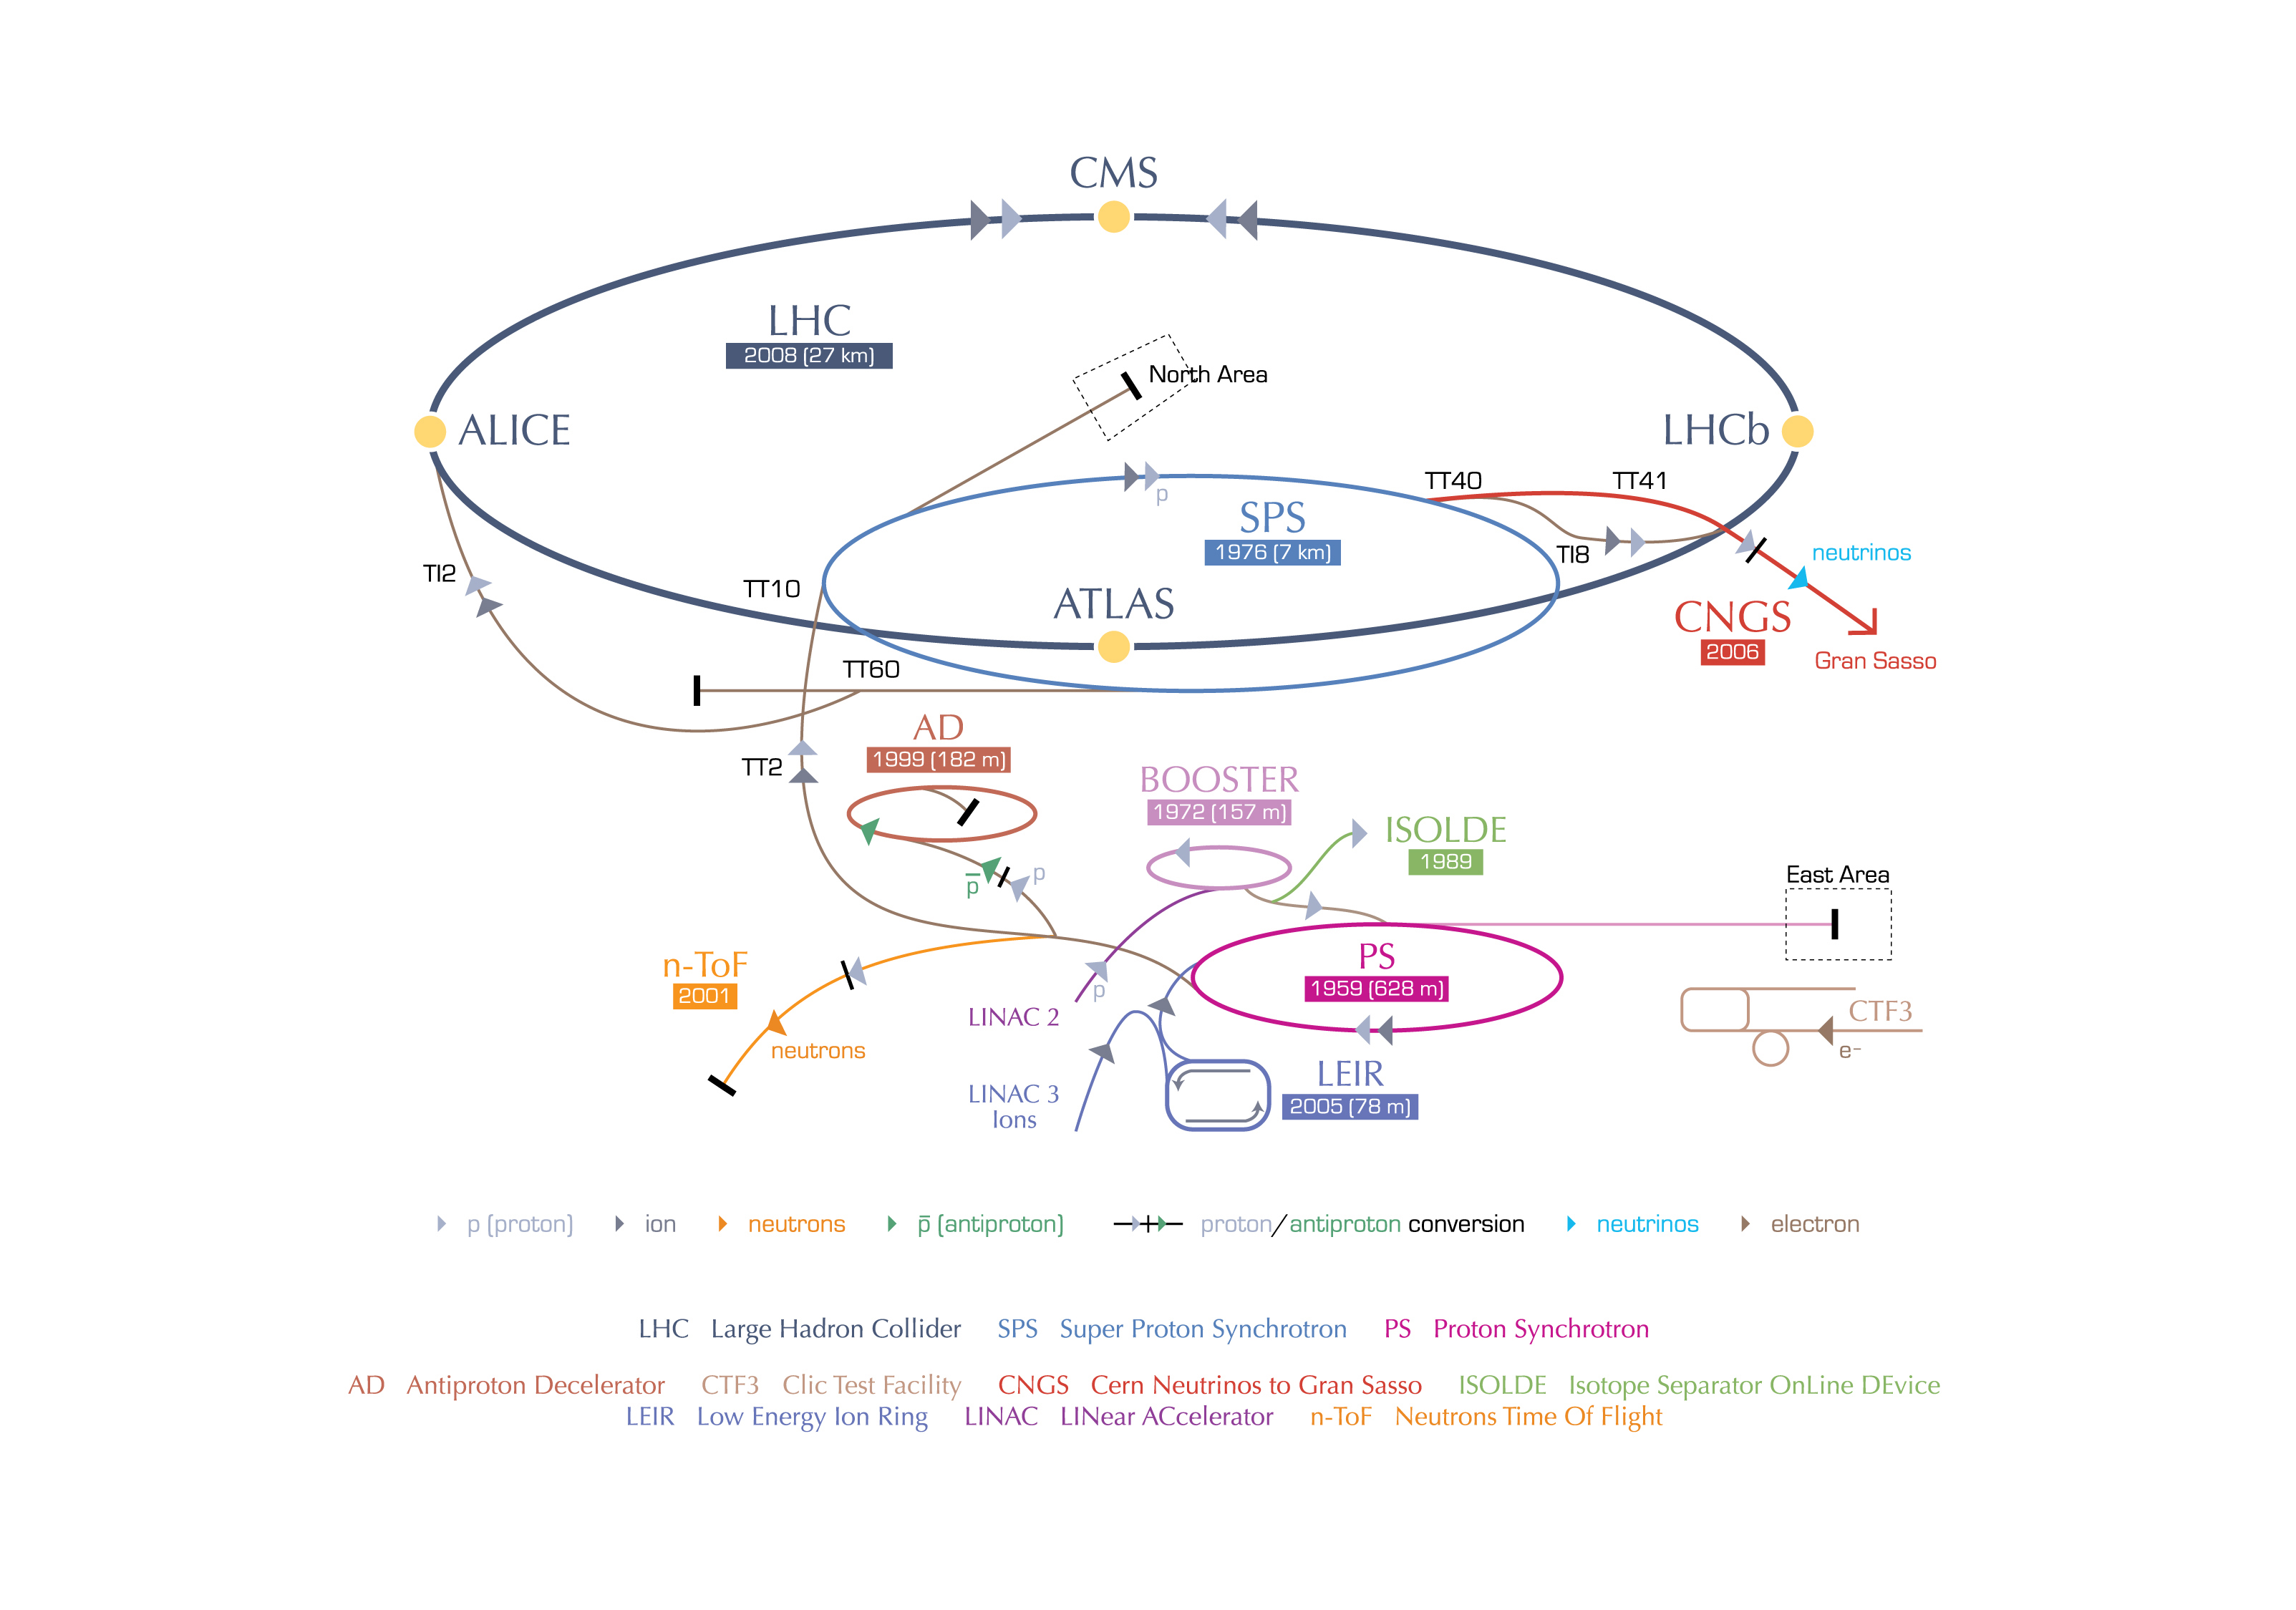
\includegraphics[width=1.0\textwidth]{figures/cms/LHC.jpg}
    \caption{The Large Hadron Collider accelerator complex. The four collision points along the ring correspond to the location of the LHC particle detectors CMS, LHCb, ATLAS and ALICE~\cite{LHC}.}
    \label{fig:cms:LHC}
\end{figure}

After the beams have reached their maximum energy and are stably circulating in the LHC ring, they are brought to collide. The goal of such a collision, which occurs every 25 nano seconds, is that some of the protons will undergo an inelastic collision, allowing the quark/gluon constituents of each proton to interact with one another and produce new and interesting particles.
The number of times such an interaction will take place inside a detector per area and time is quantified through the luminosity,$\mathcal L$, which is the proportionality factor between the number of observable events per second, and the cross section $\sigma$ of the process you are interested in
 
\begin{equation}
  \frac{dN_{events}}{dt} =\mathcal L \sigma .
\end{equation}

The cross section is the probability that an event (like one which would produce new and interesting particles) will occur and is measured in barns, where $1 \textrm{ barn} = 10^{-28} \textrm{ m}^2$. This proportionality factor should therefore be as high as possible. It depends only on parameters of the detector and can, in the case of LHC, be defined through the following accelerator quantities

\begin{equation}
  \mathcal L = \frac {N_b^2 n_b f_{rev} \gamma_r} {4 \pi \epsilon_n \beta *}F,
\end{equation}

where $N_b$ is the number of particles per bunch, $n_b$ is the number of bunches, $f_{rev}$ is their revolution frequency, $\gamma_r$ is the relativistic gamma factor,
$\epsilon_n$ is the transverse beam emittance (how confined the particles are in space and momentum), $\beta *$ is the beta function at the collision point (how narrow, or "squeezed", the beam is) and F is a reduction factor to account for a constellation where the beams do not collide heads-on but at slight crossing angles.
From this, it becomes clear that the main goal of the LHC is to; maximize the number of particles ($N_b$,$n_b$), their frequency ($f_rev$) and their energy ($\gamma_r$),
while at the same time ensuring the protons are packed together as tightly as possible (lower $\epsilon_n$ and $\beta *$).
Using the nominal values of the LHC, the peak luminosity is roughly $\mathcal L \sim 10^{34} \textrm{cm}^{-2} s^{-1}$. 


The peak luminosity of the LHC by the end of Run 2 in 2018 was grazing around $2.0 \cdot 10^{34} \textrm{cm}^{-2} s^{-1}$, corresponding to 2 times the nominal design luminosity.

To quantify the size and statistical power of a given LHC dataset, the integrated luminosity is used. This it the integral of the instantaneous luminosity over time and is defined as

\begin{equation}
  \mathcal L_{int} = \int \mathcal L dt.
\end{equation}

It is usually defined in units of inverse cross section, $\textrm{b}^{-1}$.


Despite the LHC starting up in 2008, there would be another year before data taking began.In March 2010, the LHC saw its first collision with a center-of-mass energy of 7 TeV, and continued running at this energy collecting around 5 inverse femtobarns of data by the end of 2011. In 2012, the energy was increased to 8 TeV and the LHC continued running until a planned long shutdown scheduled to begin in February 2013, collecting a total of $\sim 20 \textrm{ fb}^{-1}$ and discovering the Higgs boson. 
This marked the end of Run 1 and the beginning of a two-year maintenance project intended to prepare the LHC for running at a center-of-mass energy of 13 TeV; Run 2.

Run 2, and where this thesis begins, started in June 2015. With the accelerator now running at 90\% of its nominal energy, and with a peak luminosity between 1-2 times the design luminosity, the LHC managed to collect an impressive $\sim 160 \textrm{ fb}^{-1}$ at this energy until its planned shutdown at the end of 2018. Some key LHC accelerator parameters that were in use for the datasets analyzed in this thesis, are quoted in Table~\ref{tab:LHCparameters}

\begin{table}[]
\begin{tabular}{| l | lllll |}
\hline
Parameter               & Units                                      & Nominal & 2015 & 2016 & 2017     \\
\hline
Energy                  & {[}TeV{]}                                  & 7.0     & 6.5  & 6.5  & 6.5      \\
Bunch spacing           & {[}ns{]}                                   & 25      & 25   & 25   & 25       \\
Bunch intensity         & $\times10^{11}${[}protons/bunch{]}         & 1.15    & 1.15 & 1.15 & 1.2-1.45 \\
Bunches per train       &                                            & 144     & 144  & 96   & 144      \\
Total number of bunches &                                            & 2808    & 2244 & 2220 & 2556     \\
$\beta*$                & {[}cm{]}                                   & 55      & 80   & 40   & 27/25    \\
Peak luminosity         & $\times 10^{34} [\textrm{cm}^{-2} s^{-1}]$ & 1.0     & 0.5  & 1.4  & 2.0      \\
Integrated luminosity   &                                            &         & 4.2  & 39.7 & 50.2     \\
\hline
\end{tabular}
\caption{Some key LHC detector parameters achieved during the first years of 13 TeV data taking}
\label{tab:LHCparameters}
%https://indico.cern.ch/event/663598/contributions/2782540/,https://indico.cern.ch/event/580313/contributions/2359285/attachments/1396590/2135891/Operation_in_2016_v1_1.pdf, http://iopscience.iop.org/article/10.1088/1748-0221/3/08/S08001/pdf
\end{table}


\section{The CMS detector}

The Compact Muon Solenoid (CMS) detector is true to its name; with a diameter of 15 meters and a weight of 14000 tons, it is 60 \% smaller but two times heavier than its general purpose counterpart, the ATLAS detector.
Its large weight is due to the CMS housing the worlds largest and most powerful solenoid: A superconducting niobium titanium coil circulating 18500 Amps and capable of generating a magnetic field of 3.8 Tesla. Together with its corresponding iron return yoke, responsible for reflecting the escaping magnetic flux, it accounts for 90\% of the total detector weight.
The CMS detector is cylindrically symmetric and organized in the following way: closest to the beam pipe and at a radius of about 3 cm, the inner tracking system begins. It consists of an inner silicon pixel detector and an outer silicon strip tracker, stretching out to a radius of roughly 1.2 meters. Following the tracker are two calorimeter layers: the electromagnetic calorimeter (ECAL) consisting of lead tungstate scintillating crystals and responsible for measuring the energy of electromagnetically interacting particles, followed by the hermetic hadronic calorimeter (HCAL) measuring the energy of hadrons.
Contrary to "standard" configurations for general purpose detectors, the CMS calorimeters are located inside the superconducting solenoid. This allows the detector to be rather compact, by reducing the necessary radius of the calorimeters, and additionally for the magnet to be strong enough (the magnetic field strength depends on the coil radius) to allow muon detectors to be located within the magnetic field so their momentum can be measured.
The muon detectors are alternated with three layers of steel return yoke responsible for containing and reflecting the magnetic field and which only allows muons and weakly interacting particles to pass. A schematic overview of the CMS detector is shown in Figure~\ref{fig:cms:CMS}. In the following, the different sub-detectors will be described in detail.

\begin{figure}[h] 
    \centering
    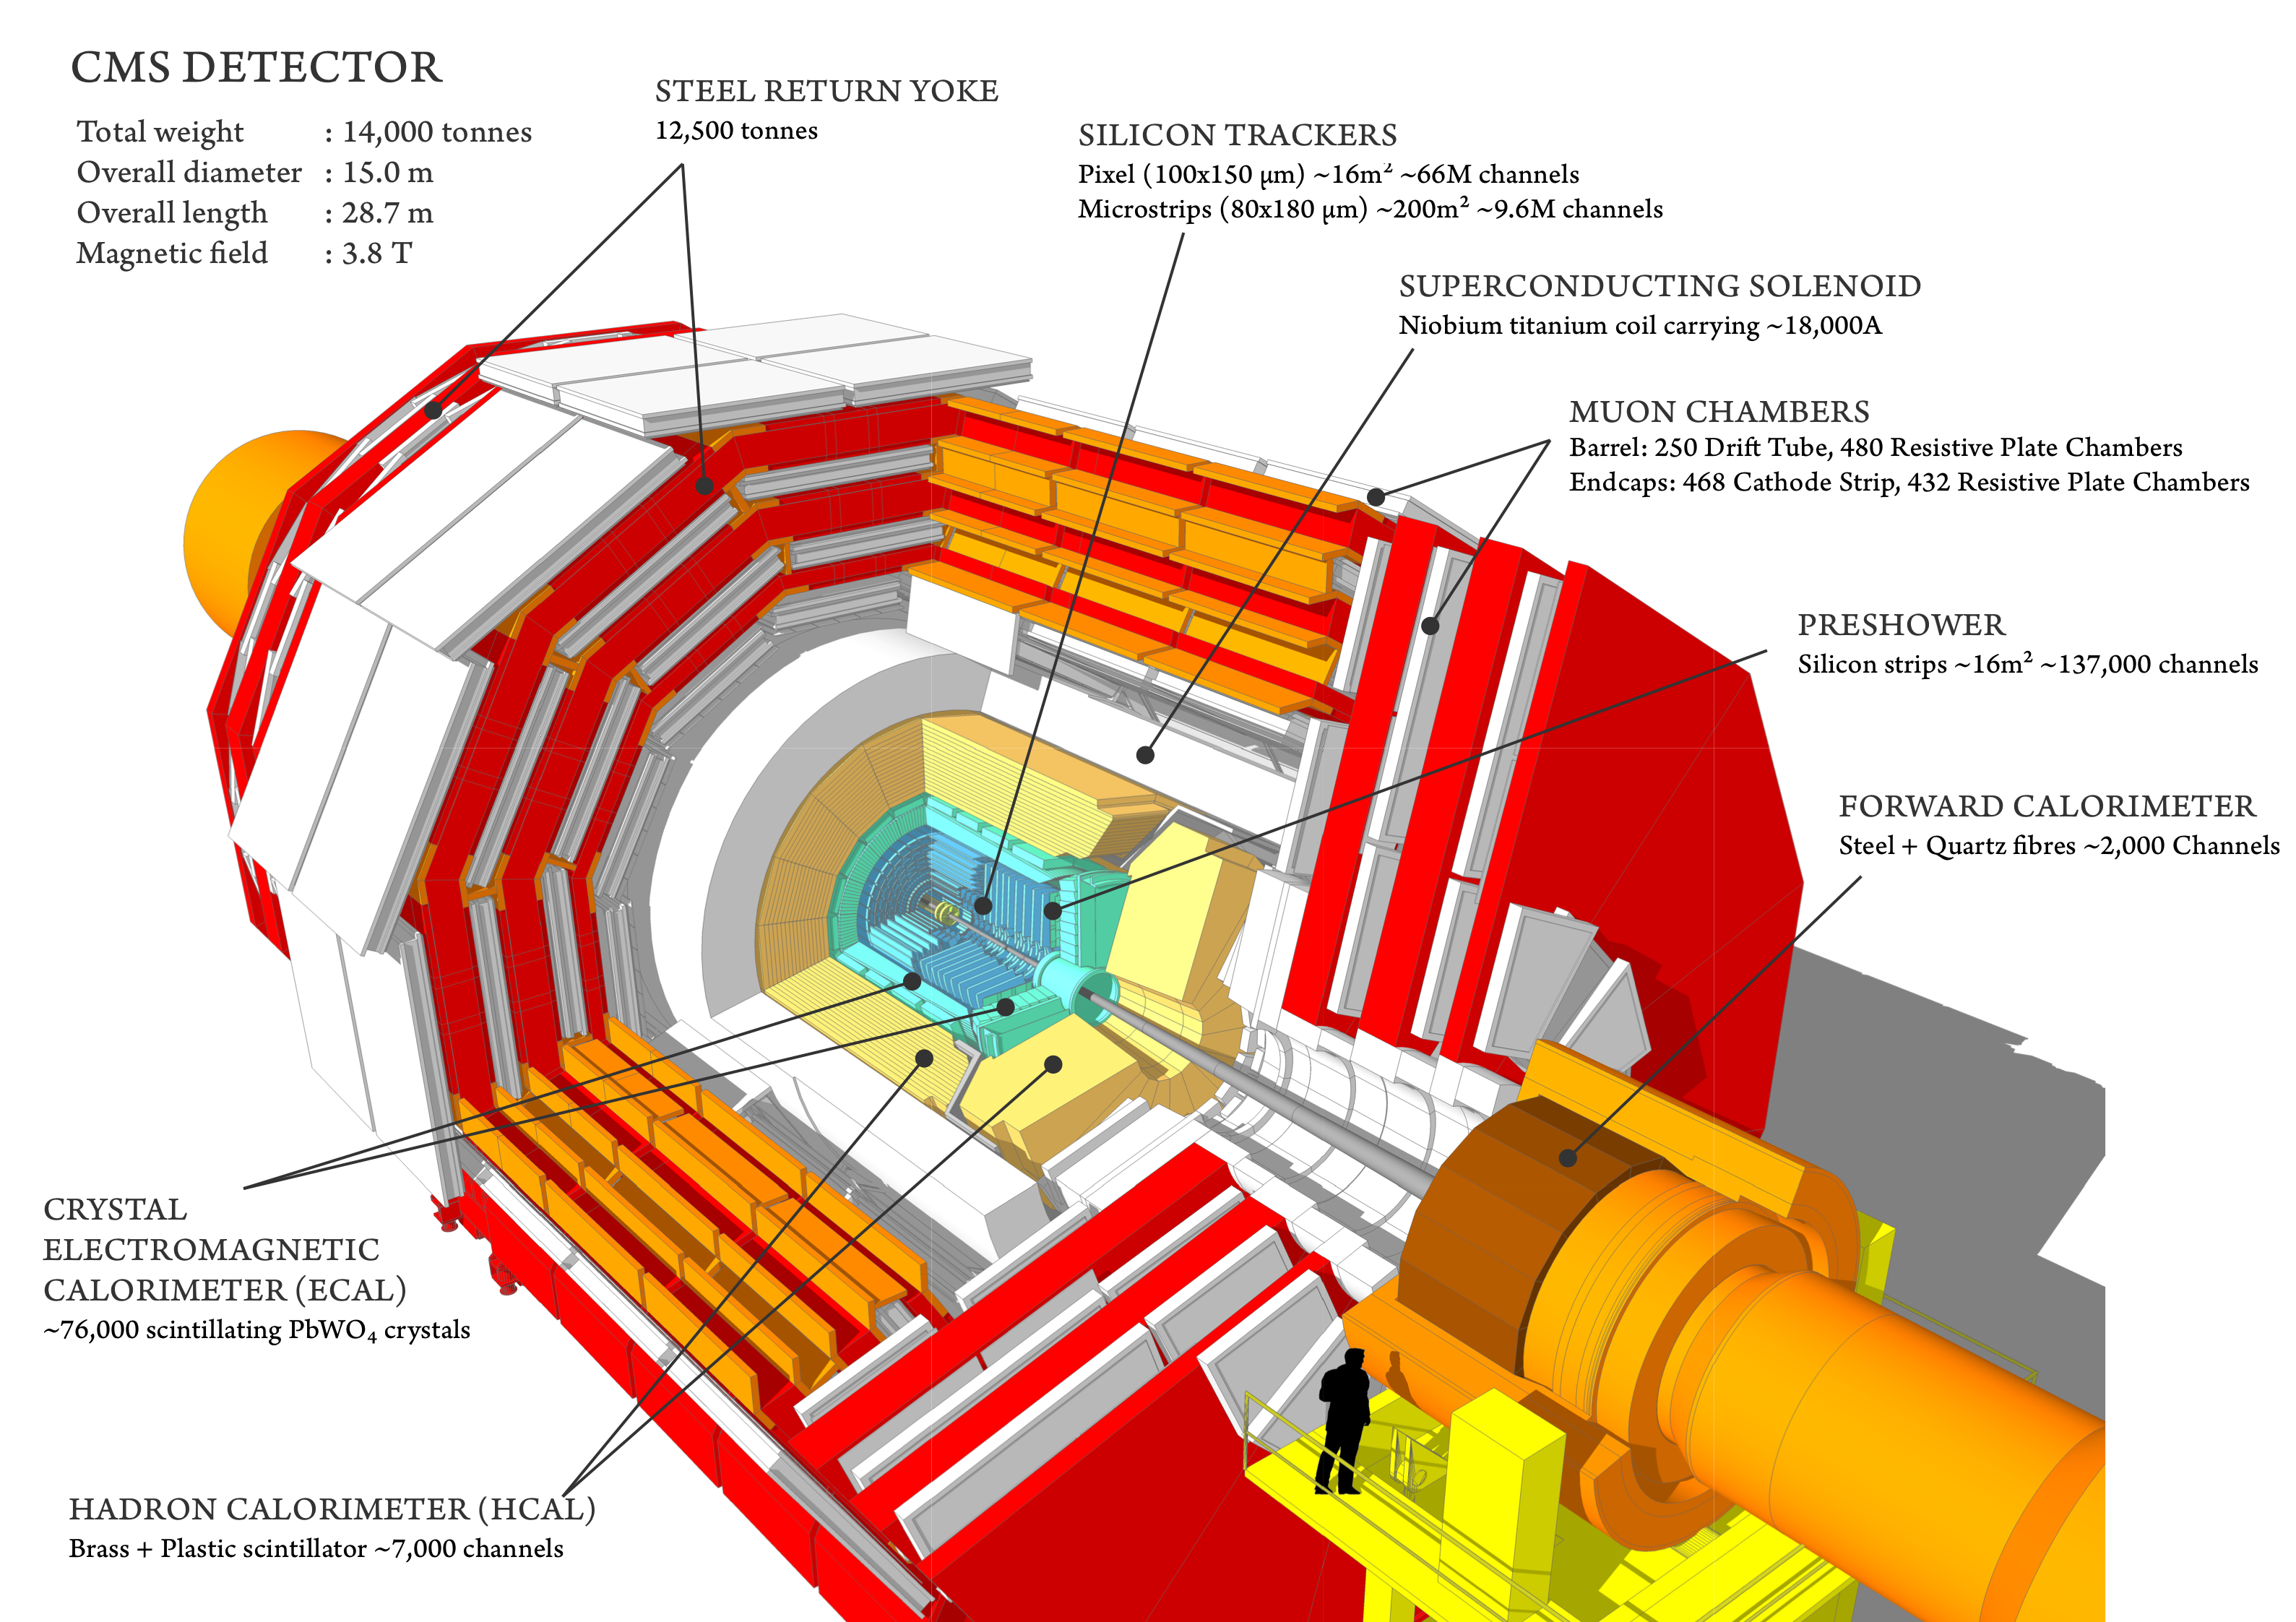
\includegraphics[width=1.0\textwidth]{figures/cms/CMS.png}
    \caption{The CMS detector and its subsystems: The silicon tracker, electromagnetic and hadron calorimeters, the superconducting solenoid and the muon chambers inter-layered with the steel return yoke~\cite{CMS}.}
    \label{fig:cms:CMS}
\end{figure}

\subsection{Coordinate system}
To describe locations within the CMS detector, a Euclidian space coordinate system is used. Here, the positive z axis points along the beam pipe towards the west, the positive x axis points towards the center of the LHC ring, and the positive y axis upw towards the earths surface. Due to the cylindrical symmetry of the detector, polar coordinates are more convenient and most frequently encountered. In this scheme, the azimuthal angle $\phi$ is measured in the xy-plane, where $\phi=0$ correspond to the positive x axis and $\phi=\pi/2$ correspond to the positive y axis. The polar angle $\theta$ is measured with respect to the z axis, $\theta=0$ aligning with the positive and $\theta=\pi$ with the negative z axis.
To define a particles angle with respect to the beam line, the pseudorapidity $\eta = -\ln{}\textrm{tan}(\theta/2)$ is preferred over $\theta$. This is due to the fact that particle production is approximately constant as a function of pseudorapidity and, more importantly, because differences in pseudorapidity are Lorentz invariant under boosts along the z-axis when assuming massless particles.
To measure angular difference between particles in the detector, the variable $\textrm{R}=\sqrt{\eta^2+\phi^2}$ is used, again Lorentz invariant under longitudinal boosts. A summary of the CMS coordinate system together with some example values are shown in Figure~\ref{fig:cms:coordinates}.


\begin{figure}[h] 
    \centering
    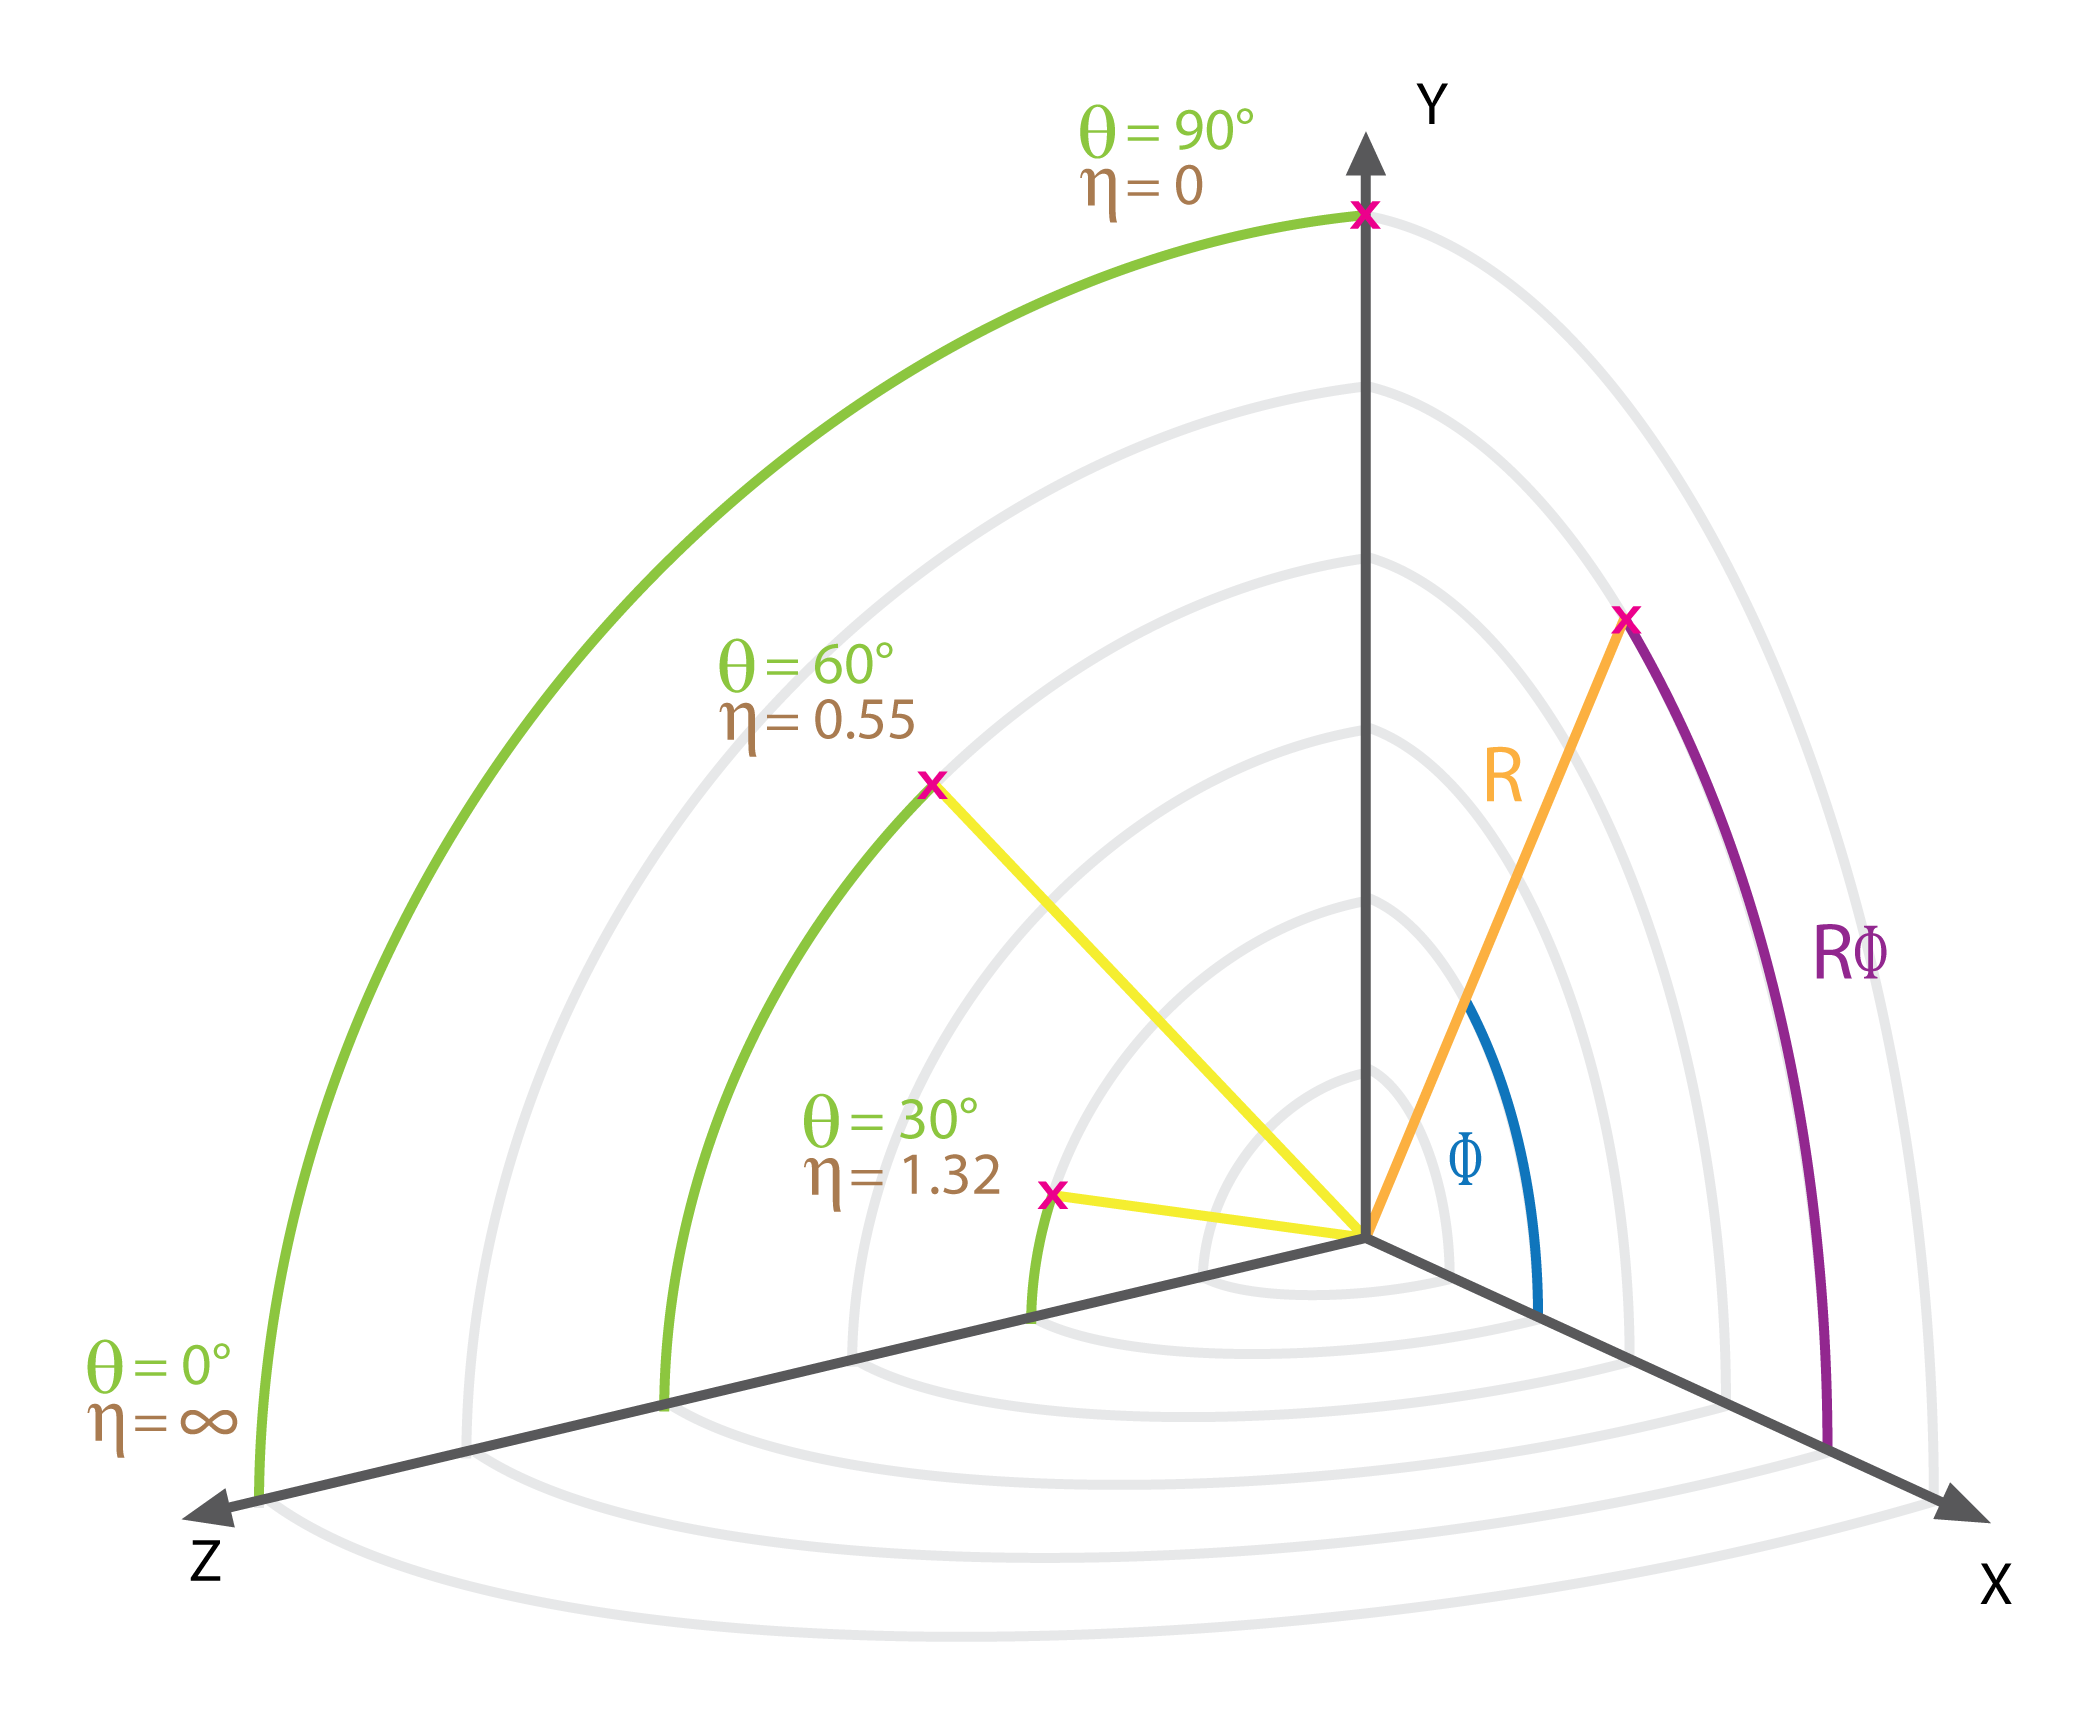
\includegraphics[width=0.45\textwidth]{figures/cms/img_cms_coordinates.png}
    \caption{The CMS coordinate system~\cite{Lenzi:2013xpa}}
    \label{fig:cms:coordinates}
\end{figure}


\subsection{Tracking detectors}
The CMS tracker is responsible for accurately reconstructing the momentum of charged particles and consists of two sub-detectors. Closest to the interaction point, and where the particle intensity is the highest, the silicon pixel detector is located. Upgraded in 2017, from the so-called Phase-0 to the Phase-1 layout, it is structured in four cylindrical barrel layers at radii 2.9, 6.8, 10.9 and 16.0 cm (the barrel pixel) and three disks in each of the forward regions placed at a distance from the nominal interaction point of 29.1, 39.6 and 51.6 cm (the forward pixel). A sketch of the current Phase-I pixel detector compared to the Phase-0 detector is shown in Figure~\ref{fig:cms:pixel}. The sensors located closest to the beam pipe are subject to hit intensities of $\mathcal{O}( \textrm{MHz}/\textrm{mm}^2 )$ which puts strict constraints on the maximum sensor size in order to minimize occupancy in the detector. The pixel sensors are \SI{100}{\micro\metre} x \SI{150}{\micro\metre} with a thickness of \SI{285}{\micro\metre}, and when counting both barrel and pixel sensors, sum up to a total of 79 million. The pixel sensors are mounted on detector modules with 16 read-out chips each, where the type of read-out chip depends on how close the module is to the beam pipe: the inner layer uses read-out chips with a rate capability of 600 MHz/$\textrm{cm}^2$ while for the outer layers, read-out chips with a rate capability of up to 200 MHz/$\textrm{cm}^2$ are sufficient.

\begin{figure}[h] 
    \centering  
    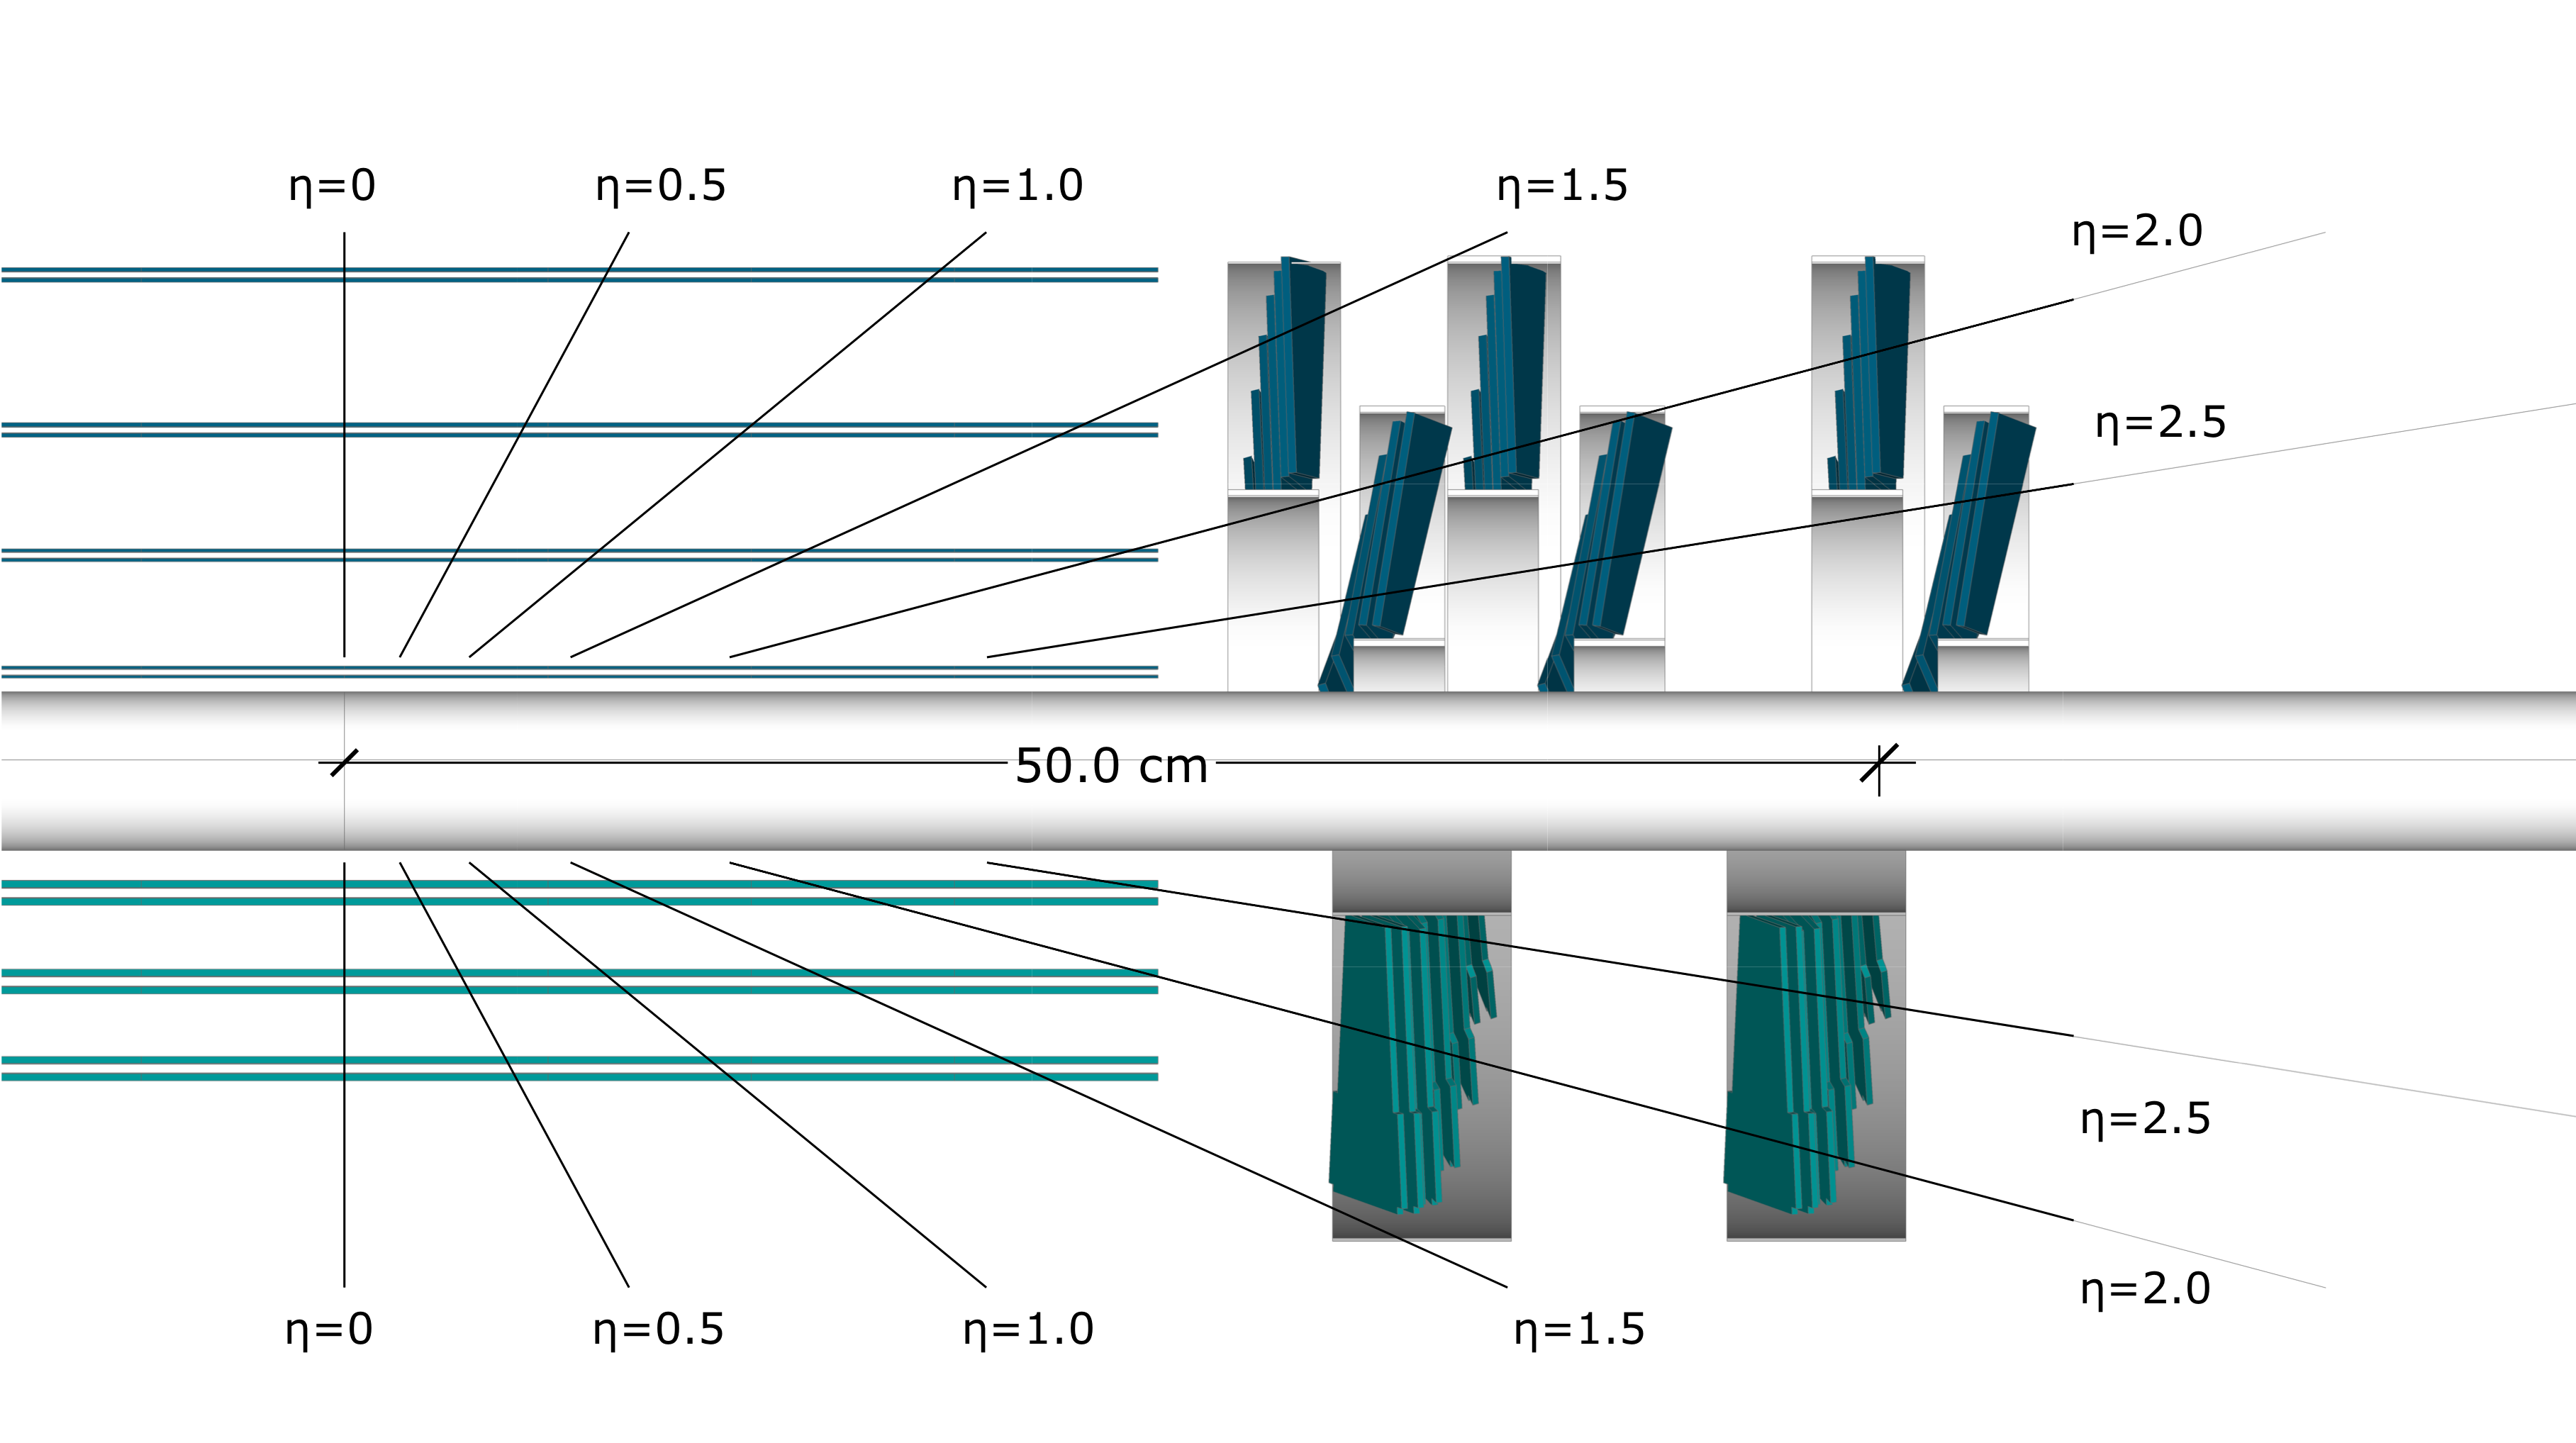
\includegraphics[height=4cm,keepaspectratio]{figures/cms/20120828_01_pixel_phase1_largesharp.png}
    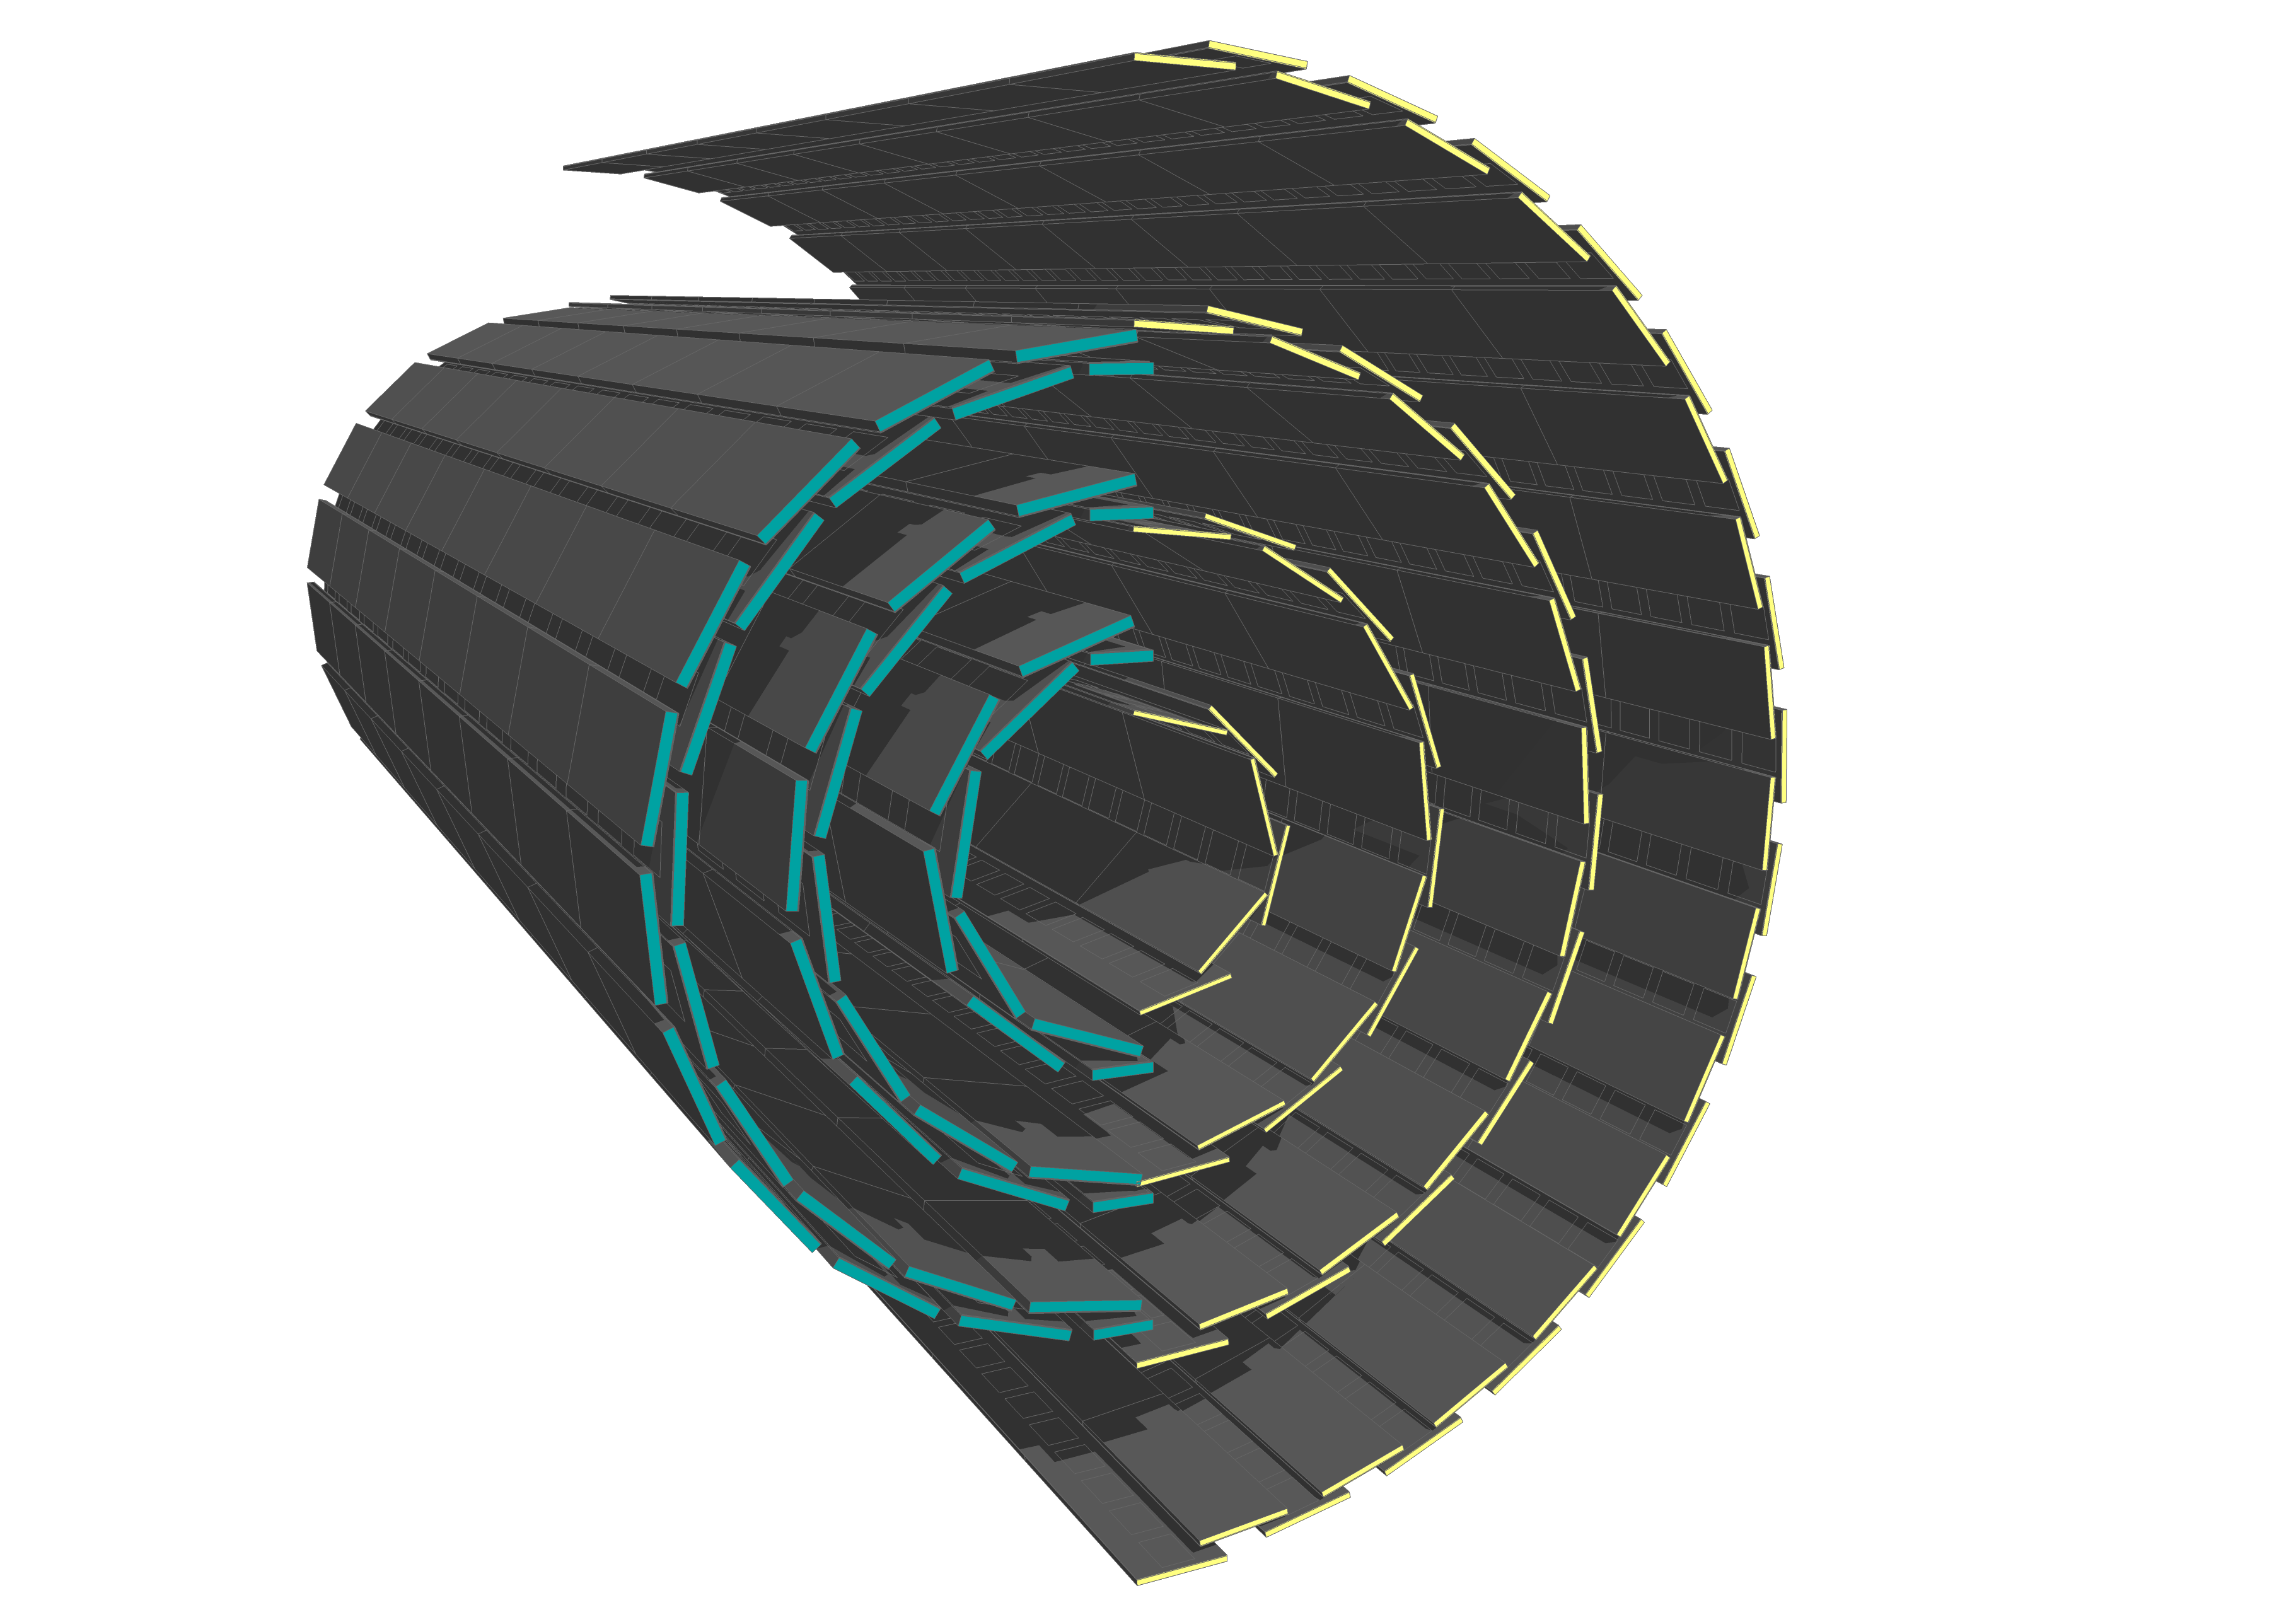
\includegraphics[height=4cm,keepaspectratio]{figures/cms/20120827_01_pixel_phase1_04.png}
    \caption{Left: The forward pixel detector layout before (bottom) and after (top) the Phase-I upgrade. Right: The barrel pixel detector before (left) and after (right) the Phase-I upgrade~\cite{Dominguez:1481838}.}
    \label{fig:cms:pixel}
\end{figure}

As the hit intensity reduces as you go further away from the beam pipe, the pixel sensors are replaced by silicon strip sensors, making up the second of the two tracker sub-systems, the silicon strip tracker. There are ten strip layers in total, stretching out to a radius of roughly 130 cm. These are divided into four sections: The inner barrel (TIB) with four strip layers, the two inner endcaps (TID) consisting of three disks each, the outer barrel (TOB) consisting of 6 cylindrical layers and the two endcaps (TEC) with 9 strip layers each. A schematic overview of the strip tracker layout is shown in Figure~\ref{fig:cms:tracker}.
The strips in the TIB and TID are 10 cm long, with a width of \SI{80}{\micro\metre} and a thickness of \SI{320}{\micro\metre}. The TOB and TEC sections consist of slightly larger strips of 25 cm x \SI{180}{\micro\metre} and a thickness of \SI{500}{\micro\metre}. The strip tracker has a total of 10 million detector strips and covers an area of $\sim 200 \textrm{ m}^2$.
To prolong the silicon detector lifetime, the entire tracker (pixel and strip) is kept at a temperature of \SI{-20}{\celsius} through a liquid cooling system.
The tracker has a coverage up to $|\eta|<2.6$ and a resolution of roughly $\sigma / \PT \approx 1.5 \times 10^{-5} \PT \oplus 0.005$.

\begin{figure}[h] 
    \centering
    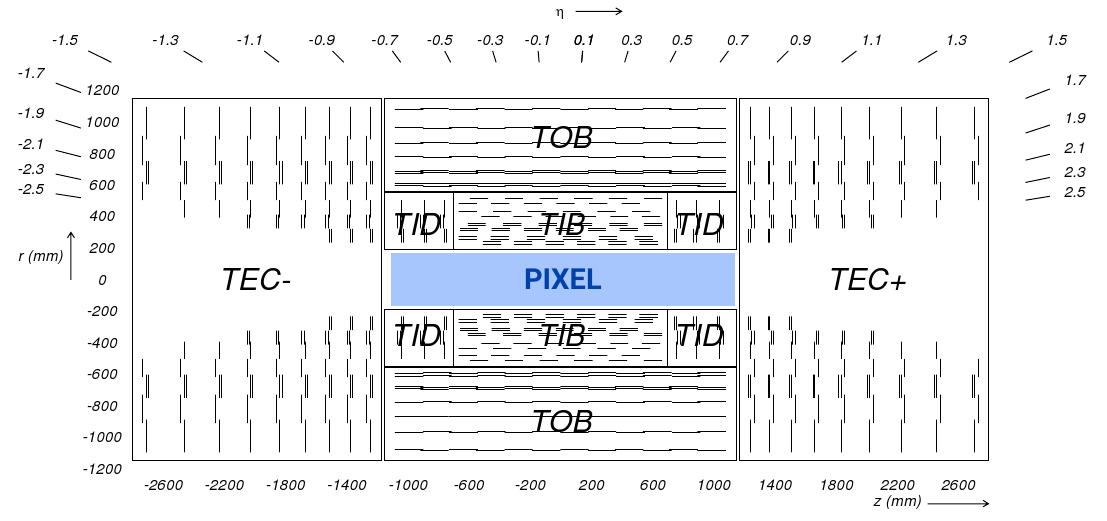
\includegraphics[width=1.0\textwidth]{figures/cms/fig_cmstracker.png}
    \caption{Schematic of the CMS silicon strip tracker and its four subsections: The inner barrel (TIB), inner endcaps (TID), the outer barrel (TOB) and the two endcaps (TEC)~\cite{Chatrchyan:2008aa}.}
    \label{fig:cms:tracker}
\end{figure}

\subsection{Electromagnetic calorimeter}
Following the tracking detectors is the electromagnetic crystal calorimeter (ECAL). Consisting of 75 848 laterally segmented scintillating lead tungstate ($\textrm{PbWO}_4$) crystals, it was designed to have the highest possible photon energy and position resolution in order to resolve a Higgs boson decaying into two photons, the cleanest of the Higgs discovery channels. 
With a goal of a photon/electron energy resolution of 0.5\% above 100 GeV, the choice of detector material for the ECAL has been its most crucial design feature. 
In order to withstand the high doses of radiation and the high magnetic field present within the detector, while at the same time generating well-defined signal responses within the 25 nanoseconds between particle collisions, an extremely dense and transparent material capable of producing fast and clean photon bursts when hit, is required. 
The choice fell on the metal heavy lead tungstate crystals. With a density of $\delta=8.28 \textrm{ g}/\textrm{ cm}^3$, the crystals are compact enough to yield excellent performance without taking up too much volume, allowing the ECAL to sit within the CMS superconducting solenoid. The homogeneous medium allows for a better energy resolution as it minimizes sampling fluctuation effects and it additionally contains enough oxygen in crystalline form to make it highly transparent to their entire scintillation
emission spectrum. With an extremely short radiation length and small Moliére radius ($\textrm{X}_0=0.85$ cm, $$\textrm{R}_M=2.19$$ cm), the required homogeneity, granularity and compactness could be achieved
Each crystal weighs around 1.5 kilogram and has a slightly tapered shape with a front face of 22 × 22 mm2 and
28.6×28.6 mm2
in the barrel and the endcaps, respectively, a fine granularity is ensured.
\subsection{Hadronic calorimeter}
\subsection{Muon chambers}
\section{Trigger system: From collision to disk}


% OBJECT RECONSTRUCTION
\chapter{Object reconstruction} %..and simulation
\label{ch:objreco}
\section{Track and primary vertex reconstruction}
The CMS tracker gets traversed by $\mathcal{O}~1000$ charged particles at each bunch crossing, produced by an average of roughly 34 proton-proton interactions happening ~simultaneously. This makes track reconstructions extremely challenging, and is the reason why a high granularity of the tracker is vital.
The average number or vertices per event for the whole Run 2 is shown in Figure~\ref{fig:objreco:pu}, with a combined average of 34 number of interactions per bunch crossing.

\begin{figure}[h] 
    \centering
    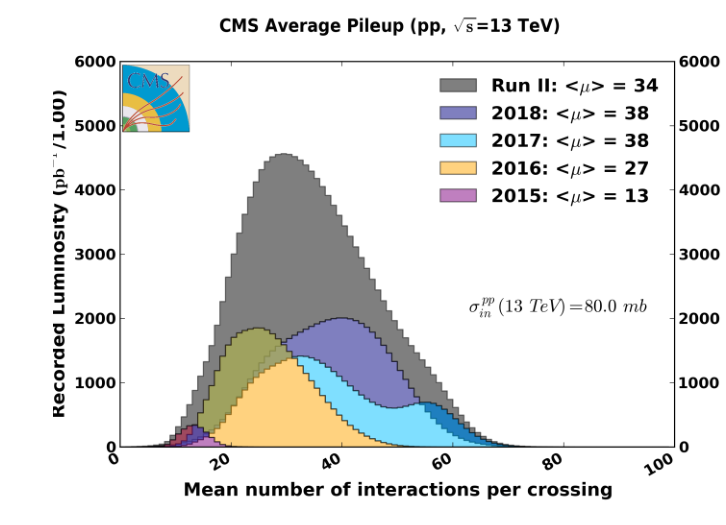
\includegraphics[width=0.49\textwidth]{figures/event_reconstruction/pu.pdf}
    \caption{The average number of vertices per event in CMS during the Run 2 datataking~\cite{CMSlumi}.}
    \label{fig:objreco:pu}
\end{figure}

Track reconstruction describes the process of taking hits from the pixel and strip detectors, combining them and estimating the momentum and flight direction of the charged particle responsible for producing the hits. It is an extremely computationally heavy process and is based on what is called a combinatorial Kalman filter~\cite{BILLOIR1989390}. A Kalman filter is an algorithm that uses time-dependent observations in order to estimate unknown variables, by proceeding progressively from one measurement to the next, improving the knowledge of the
trajectory with each new measurement. The track reconstruction software in CMS (called the Combinatorial Track Finder (CTF)) constructs its collection of tracks by iteratively looping over the hits and reconstructing tracks, then removing those which are already used as inputs for a previous track. It starts from a seed in the inner most tracker layers, usually two or three hits, and then extrapolates the seed trajectories searching for additional hits to associate to that candidate. It then disregards tracks that fail certain criteria  based on a $\chi^2$ calculation taking both hit and trajectory uncertainties into account, as well as the number of missing hits.
The track reconstruction algorithm is effective over the full tracker coverage range up to $|\eta|<2.5$ and can reconstruct particles with momenta as low as 0.1 GeV or particles which are produced up to 60 \cm from the beam line. In the central region, particles with a momentum of 100 GeV have a \PT-resolution of roughly 2.8 \%, a transverse impact parameter resolution of 10 $\micron$ and a longitudinal impact parameter of 30 $\micron$. 


In order to define the location and uncertainty of every proton-proton interaction in an event, primary-vertex reconstruction in performed. Primary vertices lie within a radius of a few millimeters of the beam axis and are defined as the common origin of groups of tracks.
The reconstruction algorithm takes as input the reconstructed tracks from the previous step which pass certain selection criteria, clusters the tracks that share a common origin and then fit for the position of each vertex. Each track must have at least 2 hits in the pixel layers and no less than 5 hits in the pixel+strip as well as a $\chi^2<20$ from a fit to the particle trajectory to be considered as input for the vertex finder. The primary vertex resolution is around 12 \micron in x and 10 \micron in z for vertices with at least 50 tracks.

Offline, all events are required to have at least one primary vertex reconstructed within a 24 \cm window along the beam axis, with a transverse distance from the nominal interaction region of less than 2 \cm. The reconstructed vertex with the largest value of summed physics object $\PT^2$ is selected as the primary interaction vertex where the hard scattering process occurred.

\section{The Particle Flow Algorithm}

After track reconstruction, what remains is an incoherent collection of tracks, calorimeter clusters and hits in the muon chambers. In order to connect these, CMS uses an algorithm called Particle Flow (PF)~\cite{1748-0221-12-10-P10003} to combine the information obtained from all sub-detectors in order to infer which particles were actually produced in the event.
The reconstructed physics object in the order of which they are reconstructed are
\begin{itemize}
  \item Muons, through hits in the tracker and in the muon chambers
  \item Charged hadrons, through hits in the tracker and energy deposits in the calorimeters
  \item Neutral hadrons, through energy deposits in the calorimeters but no hits in the tracker
  \item Photons, through energy deposits in the ECAL but not in the HCAL and no hits in the tracker
  \item Electrons, through hits in the tracker and energy deposits in the ECAL
\end{itemize}

How these different particles propagate through the CMS detector is illustrated in Figure~\ref{fig:objreco:PF}.

\begin{figure}[h] 
    \centering
    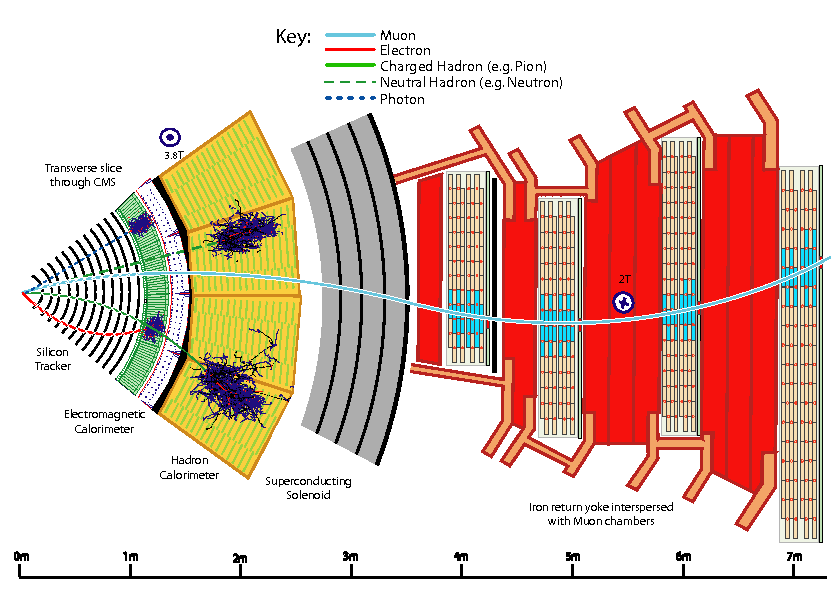
\includegraphics[width=0.79\textwidth]{figures/event_reconstruction/PF.png}
    \caption{Particle interactions in the different subdetectors for a transverse slice through the CMS detector~\cite{1748-0221-12-10-P10003}.}
    \label{fig:objreco:PF}
\end{figure} 

\subsection{Reconstruction of the Particle Flow inputs}

\subsubsection{Electron tracking}
\label{subsub:objreco:electrontracking}
Electron seeding is done in two different ways: ECAL-based  or tracker-based electron seeding. In the ECAL-based method, electrons are seeded from  ECAL clusters with $E_T > 4 \GeV$, where the position of the cluster is used to infer which hits in the inner tracker belongs to a given electron or positron. As a large fraction of the electron/positron energy is emitted through bremsstrahlung before even reaching the ECAL, ECAL superclusters covering a small window in $\eta$ and a larger window in $\phi$ are defined in order to fully contain the electron as well as its bremsstrahlung photons. As these superclusters are prone to contamination, tight isolation requirements need to be applied, leading to reconstruction inefficiencies. Therefore, an additional tracker-based seeding approach has been developed. All tracks with $\PT>2\GeV$ are used as potential electron seeds. These tracks are then extrapolated to the ECAL and matched to the closest ECAL cluster. The ratio of the cluster energy to the track
momentum is required to be ~1. The electron candidates are then fit with a Gaussian-sum filter (GSF)~\cite{0954-3899-31-9-N01} and required to pass certain criteria based on the score of a boosted-decision-tree (BDT) which combines the number of tracker hits, the $\chi^2$ of the GSF track, the energy loss along the  track, and the distance between the extrapolated track to the closest ECAL cluster.

\subsubsection{Muon tracking}
\label{subsub:objreco:muontracking}
Muon tracking consists of two part: the muon spectrometer allows muons to be identified with high efficiency over the full pseudorapidity range, while maintaining a low background due to the absorbing calorimeter layers upstream. The inner tracker on the other hand, provides an accurate measurement of the muon momentum. Three muon quality flags are defined
\begin{itemize}
  \item Standalone muon: Muon tracks based on hits in the DT or CSC only
  \item Global muon: A standalone muon track matched to a track in the tracker if the track parameters of the two are compatible
  \item Tracker muon: An inner track with $\PT> 0.5 \GeV$, a total momentum greater than 2.5 \GeV and at least one muon segment matching the extrapolated inner track
\end{itemize}
Around 99\% of muons produced within $|\eta|<2.4$ are reconstructed as a global muon or a tracker muon, and very often as both. If the global and tracker muon share the same inner tracker segment, the two are combined.

\subsubsection{Calorimeter clusters}
 The calorimeter clustering is performed separately for each calorimeter subdetector (ECAL barrel and endcaps, HCAL barrel and endcaps and the preshower layers).
The first step is to define cluster seeds from cells with an energy exceeding some predefined threshold and in addition is larger than the energy in its neighboring cells. Topological clusters are then formed by adding cells to the seed which has at least one corner in common with a cell already in the cluster, and that has an energy which is at least twice the noise level of the detector. In Figure~\ref{fig:objreco:caloclustering}, an example of calorimeter clustering for a five-particle jet is shown for the HCAL (left) and ECAL (right). In the HCAL (left), two seeds have been identified (gray filled areas) inside a topological cluster consisting of 9 cells. These are then defined as two HCAL clusters, with a position as indicated by the red circles. The green solid lines correspond to charged tracks reconstructed in the tracker, both pointing to the center of the HCAL cluster seeds. The observed deposits left by the same particles are shown on the right in Figure~\ref{fig:objreco:caloclustering}, where the $K^0_L$, $\pi^-$ and the two photons from the decay of a $\pi^0$ leave distinct clusters in the ECAL. The $\pi^+$ leaves no energy deposit in this case. 

\begin{figure}[h] 
    \centering
    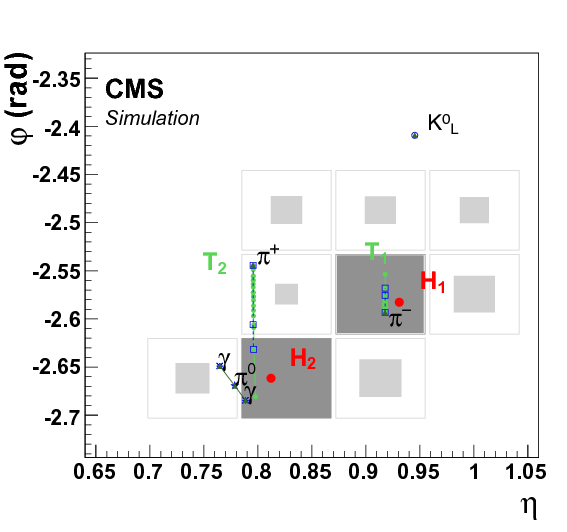
\includegraphics[width=0.49\textwidth]{figures/event_reconstruction/PF_HCAL.png}
    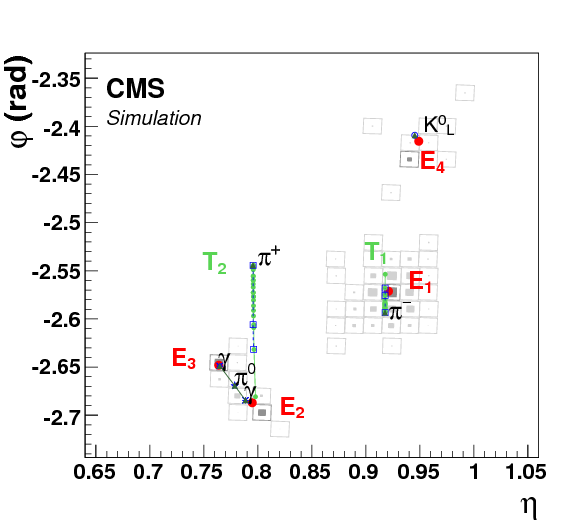
\includegraphics[width=0.49\textwidth]{figures/event_reconstruction/PF_ECAL.png}
    \caption{The $\eta-\phi$ vies of calorimeter clusters generated by a five-particle jet in the HCAL (left) and in the ECAL (right). The squares correspond to calorimeter cells, where the inner area is proportional to the logarith of the cell energy. Cluster seeds are depicted in dark gray. The dotted blue lines correspond to the simulated particle trajectory, while the green lines correspond to charged tracks reconstructed in the tracker~\cite{1748-0221-12-10-P10003}.}
    \label{fig:objreco:caloclustering}
\end{figure} 


\subsection{Particle Flow identification}

\subsubsection{The link algorithm}

The link algorithm is the algorithm responsible for combining the particle flow elements from different subdetectors.
It can test any pair of elements in the event based on specific requirements depending on the nature of the element, but is restricted to the nearest neighbors in the $\eta-\phi$ plane.
The outputs of the link algorithm are so-called \textit{PF blocks} of linked elements, either directly linked or linked through having common elements.
\begin{itemize}
  \item \textbf{Inner track - calorimeter cluster link:} The track is interpolated from its last hit, through the preshower layers, the ECAL and ending in the HCAL at an interaction length depth of 1. A link is made if the track is within the cluster area, where the areas is enlarged by up to a cell in each direction to account for detector gaps. In case several ECAL/HCAL clusters are linked to the same track, only the one with the smallest distance in $\eta-\phi$ is kept.

\item \textbf{Calorimeter cluster - cluster link:} A link between ECAL and HCAL clusters as well as between ECAL and preshower clusters
is made when the cluster position of the more granular calorimeter is within the cluster envelope in the less granular calorimeter. Also here, if there is link overlap, only the link with the smallest distance is kept

\item \textbf{Inner tracker -muon chamber link:} As described in Section~\ref{subsub:objreco:muontracking} 
\end{itemize}

For each PF block, the reconstruction proceeds in the following order.
First, muons are reconstructed and their corresponding PF elements removed from the PF block. Then the electrons are reconstructed, with the hopes of removing their corresponding bremsstrahlung photons from the list of PF elements. Energetic photons are reconstructed in the same step. Finally, neutral and charged hadrons are reconstructed.

\subsubsection{Muons}

First, isolated global muons are selected by requiring the sum of track \PT and calorimeter energy deposits within a cone of $\Delta R = 0.3$ not belonging to the muon track, to be smaller than 10 \% of the muon \PT.
If the muons are non-isolated, they are required to pass the tight muon requirement~\cite{1748-0221-7-10-P10002} and have at least three matching track segments in the muon detector or have matched calorimeter deposits compatible with being a minimum ionizing particle.
Muons failing both the requirements above are kept if the standalone muon track is of high quality and have a lot of hits in the muon detectors, otherwise they are discarded.
The muon momentum is defined from the inner tracker measurement if the muon \PT is less than 200 \GeV. Otherwise, its chosen according to the track fit with the smallest $\chi^2$ probability.

\subsubsection{Electrons}
The electrons are seeded from a GSF track, as described in Section~\ref{subsub:objreco:electrontracking}. To differentiate electrons from charged hadrons, the energy deposit in the HCAL within a distance of 0.15 in the $\eta-\phi$ plane of the supercluster , is required to be less than 10 \% of that of the supercluster. The electron candidate must further pass a requirement on the output of a dedicated electron-identification BDT, using inputs such as track-cluster distance, track $\chi^2$ and number of hits as input.  In this step, isolated photons are also reconstructed, seeded from ECAL superclusters with $|E_T>10 \GeV|$ and no link to a GSF track.
All the tracks and calorimeter deposits used to reconstruct electrons and isolated photons are further removed from the list of PF blocks.

\subsubsection{Hadrons}
Finally, after the removal of muons and electrons, the remaining hadrons and non-isolated photons are identified. HCAL clusters with no track link are defined as neutral hadrons, while ECAL clusters with no track link are defined as photons (photons are exclusively associated to the ECAL deposits as neutral hadrons leave only 3 \% of their energy in the ECAL).
The remaining HCAL clusters are then linked to one or more tracks from the inner tracker. In order to determine the particle content within a cluster, the sum of track momenta and the calorimeter energy is compared.If the calorimeter energy is compatible with the sum of track momenta, a particle for each track is inferred, with its corresponding energy taken from the track momentum.  If the calorimeter energy is larger than the sum of track momenta, a photon or a neutral hadron is added, togehter with one charged hadron for each track within the cluster area.

\section{Pile-up removal}

Particles originating from proton-proton interactions not associated with the hardest primary vertex, are denoted pileup events.
These distorts observables of interest from the hard scattering event and must be mitigated through dedicated pileup removal techniques

\subsection{Charged Hadron Subtraction}
\label{subsub:objreco:chs}
As mentioned previously, primary vertices are reconstructed using tracks from charged hadrons. If a primary vertex does not correspond to the hard scattering vertex of the event, the charged hadrons (as reconstructed through Particle Flow) associated to this vertex (called pileup vertex) are removed from the event collection of particles and will not participate in any further object reconstruction. This method is denoted charged hadron subtraction (CHS).

\subsection{Pile up per particle identification (PUPPI)}
\label{subsub:objreco:puppi}
CHS was the default pileup removal algorithm in CMS until very recently. In 2014, a new pileup removal algorithm with improved performance was proposed; the pileup per particle identification (PUPPI)~\cite{Bertolini2014} algorithm.
PUPPI uses a combination of local shape information, event pileup properties and tracking information to compute a weight describing the degree of "pileup-likeness" of a given particle.
First, a variable denoted $\alpha$ is computed based on the difference between soft radiation coming from pileup and the harder collinear QCD pattern. The shape of $\alpha$ for charged particles is then used as a proxy for all pileup particles and is used on an event-by-event basis to calculate a weight for each particle. This weight in turn describes the degree to which particles are pileup-like and are used to rescale the particle four-momenta.

The shape variable for a given particle $i$ is defined as

\begin{equation}
  \alpha_i = \log \sum_{\substack{j \in \mathrm{Ch,PV} \\ j \neq i}} \left(\frac{p_{T,j}}{\Delta R_{ij}}\right)^{2} \Theta(R_0 - \Delta R_{ij}),
\end{equation}

where $\Theta$ is the step function and $j$ refers to the neighboring charged particles from the primary vertex within a cone of radius $R_0=0.4$. Charged particles are defined as coming from the primary vertex if they are associated to the leading vertex of the event or are within a distance of $d_z < $0.3~\cm from the leading vertex. 

In order to determine the probability that a particle comes from pileup, a $\chi^{2}$ calculation is performed. The probability is defined as

\begin{equation}
\chi^{2}_{i} = \frac{(\alpha_i -  \bar{\alpha}_{PU})^{2}}{RMS_{PU}^{2}},
\end{equation}

where $\bar{\alpha}_{PU}$ is the median value of the $\alpha_i$ distribution for pileup particles in the given event and $RMS_{PU}$ is its RMS.

Each particle (neutral and charged) is then assigned a weight $w_i = F_{\chi^2,NDF=1}(\chi^2_i)$, where $F_{\chi^2,NDF=1}$ is the cumulative distribution function of the $\chi^2$ distribution with one degree of freedom. Particles with $w_{i}<0.01$ are rejected.
In addition, a cut on the weighted \PT of neutral particles of $w_{i} \cdot p_{T,i} >  (A + B \cdot N_{PV})$ \GeV is applied, where $N_{PV}$ correspond to the number of reconstructed vertices in the event and A and B are tunable parameters. 

The performance of the PUPPI algorithm compared to CHS for jet observables is shown in Figure~\ref{fig:objreco:puppi}.

\begin{figure}[ht] 
    \centering
    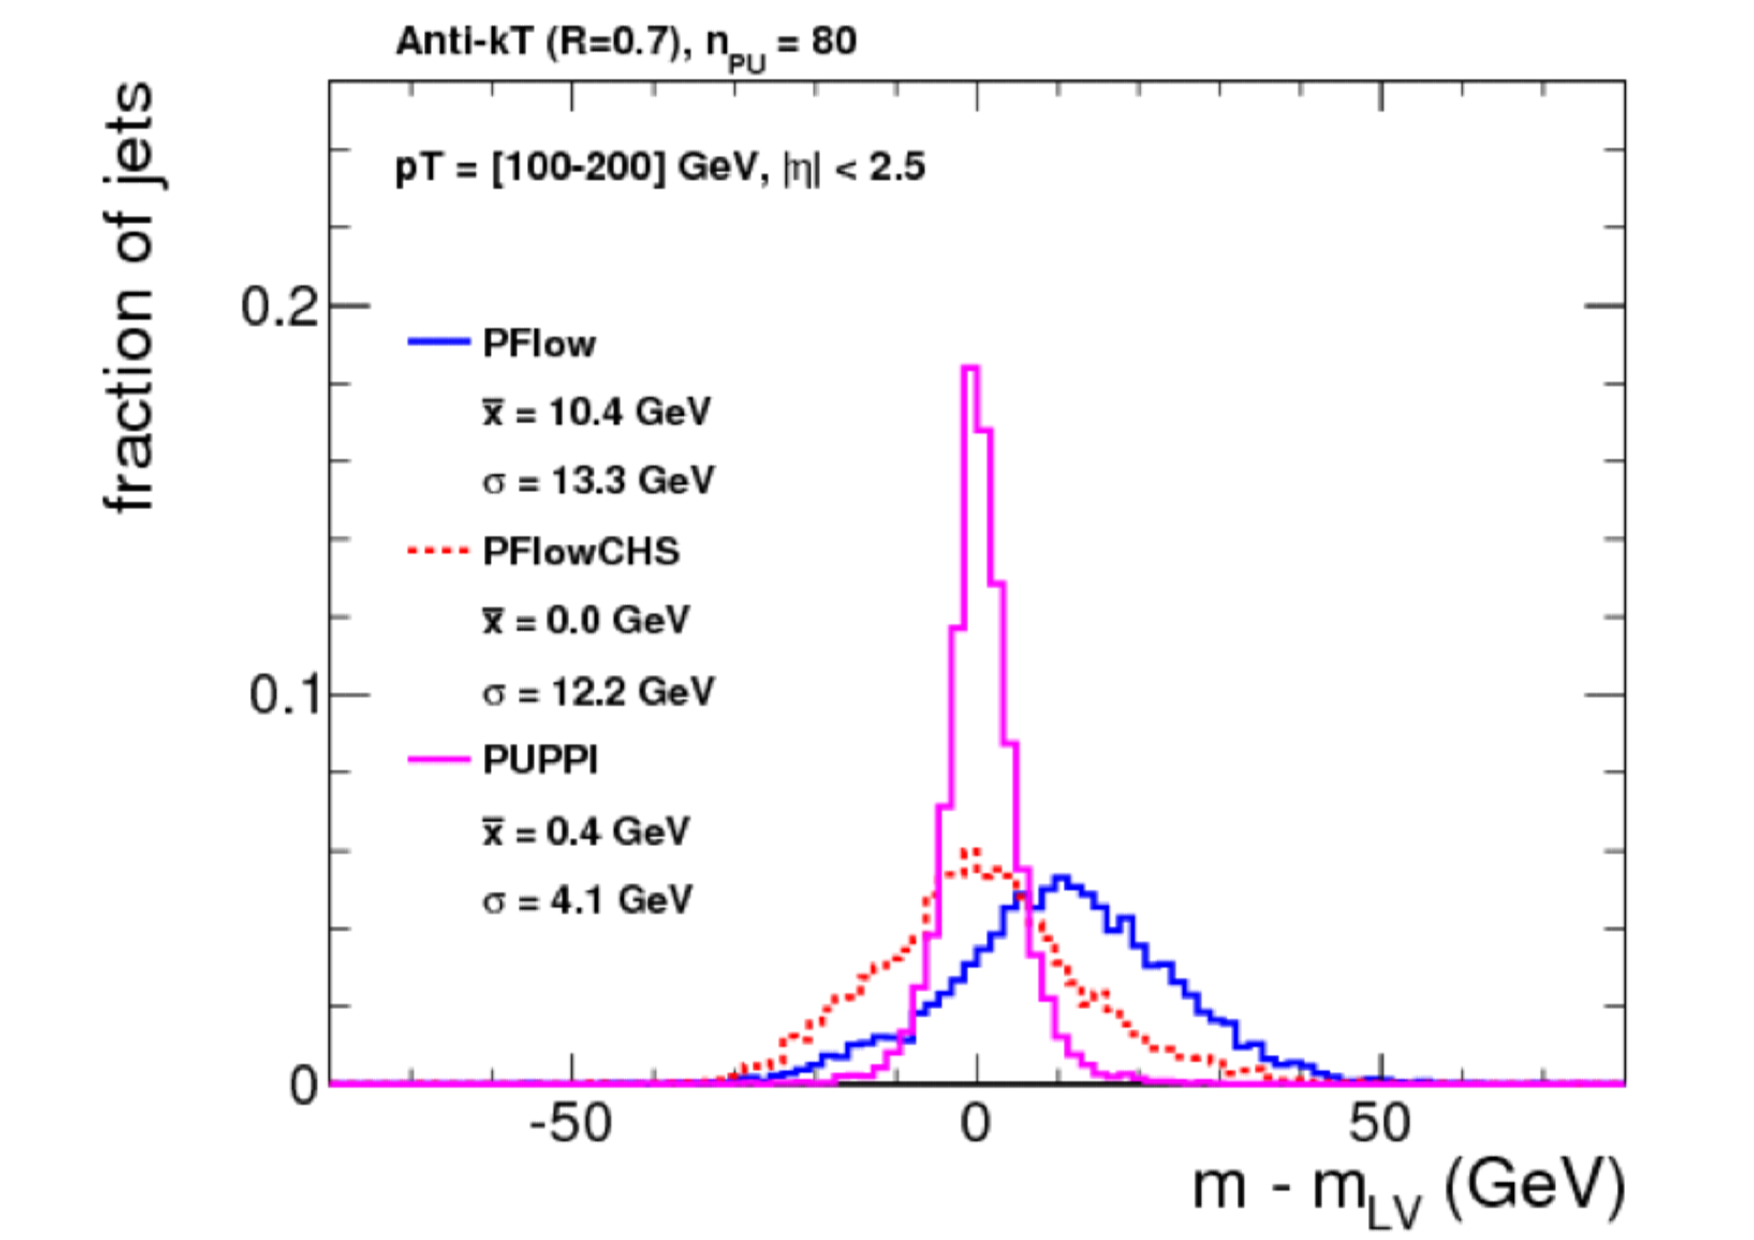
\includegraphics[height=5cm]{figures/event_reconstruction/puppi_mres_hiPt.pdf}
    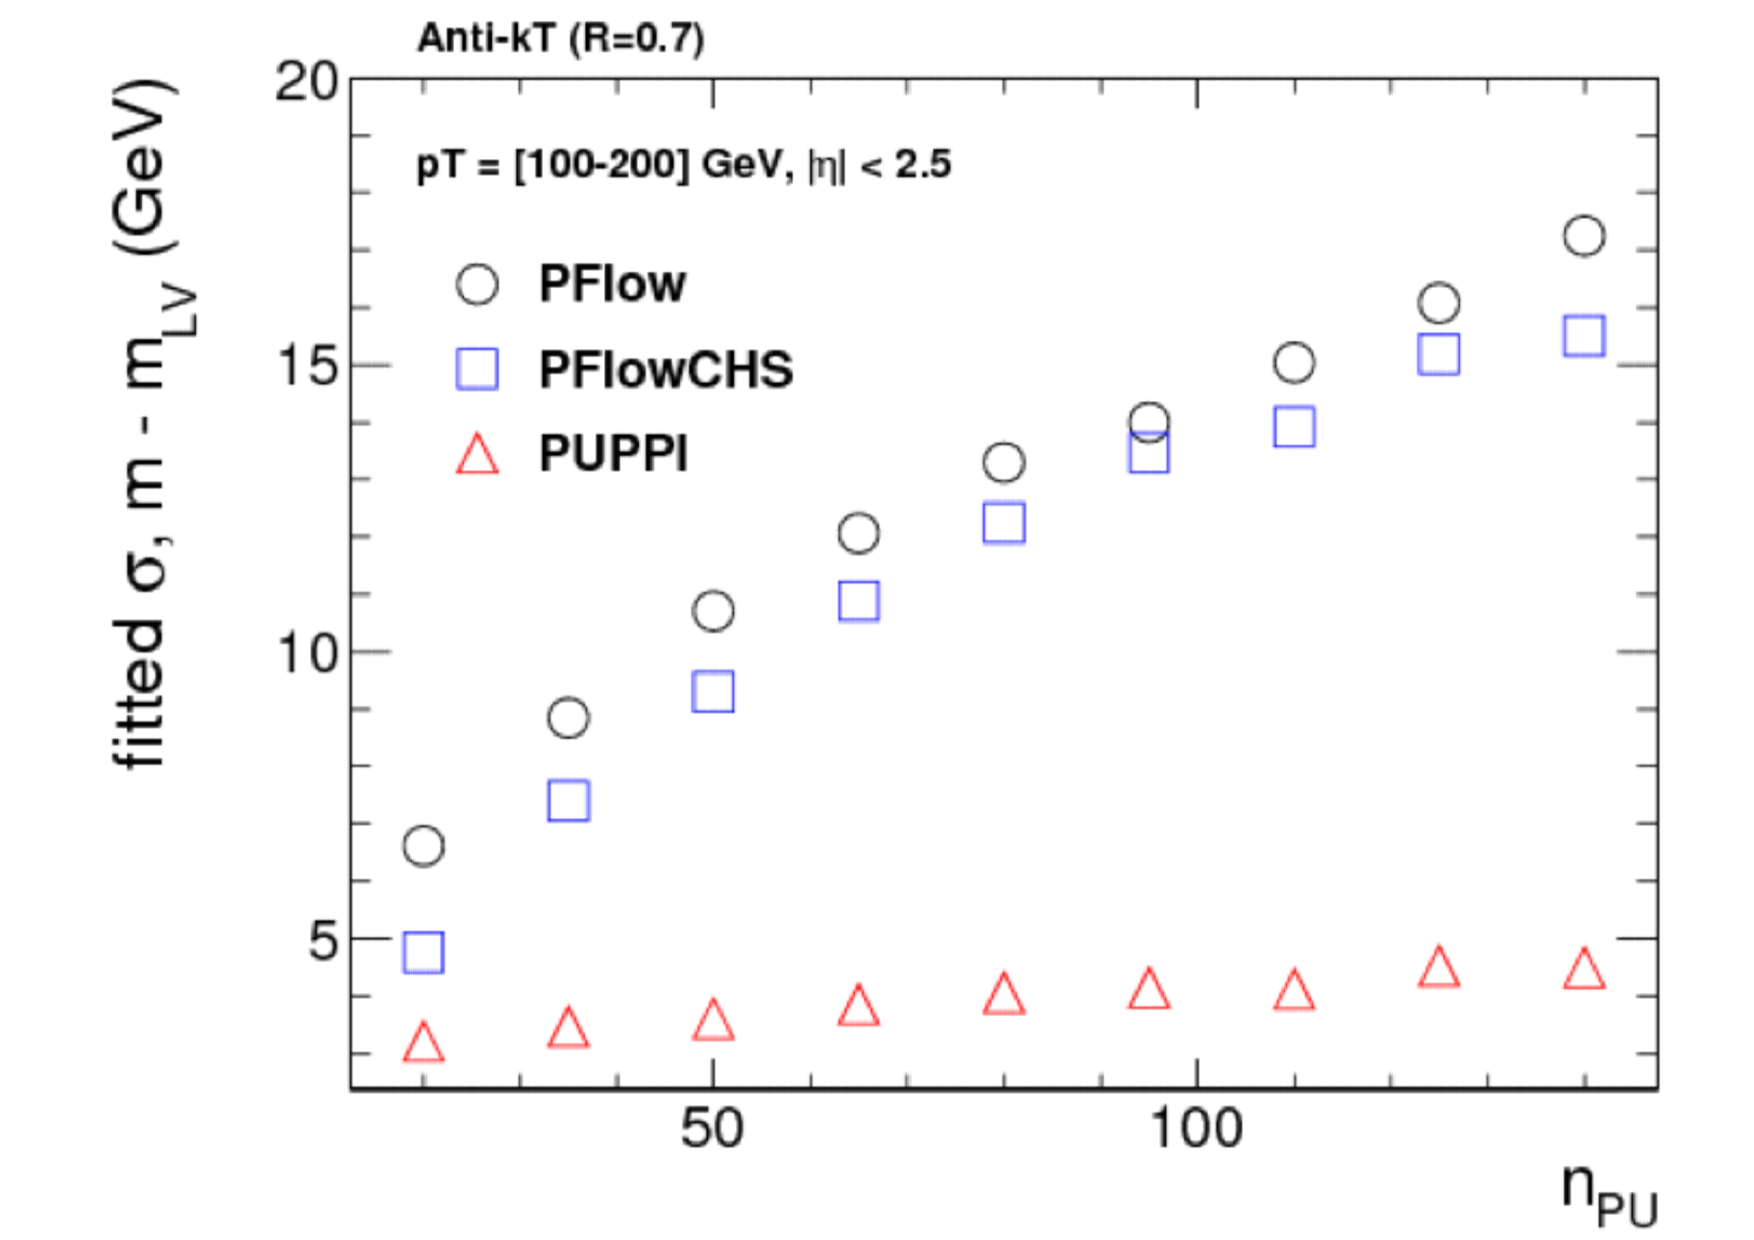
\includegraphics[height=5cm]{figures/event_reconstruction/puppi_mresVsPu.pdf}\\
    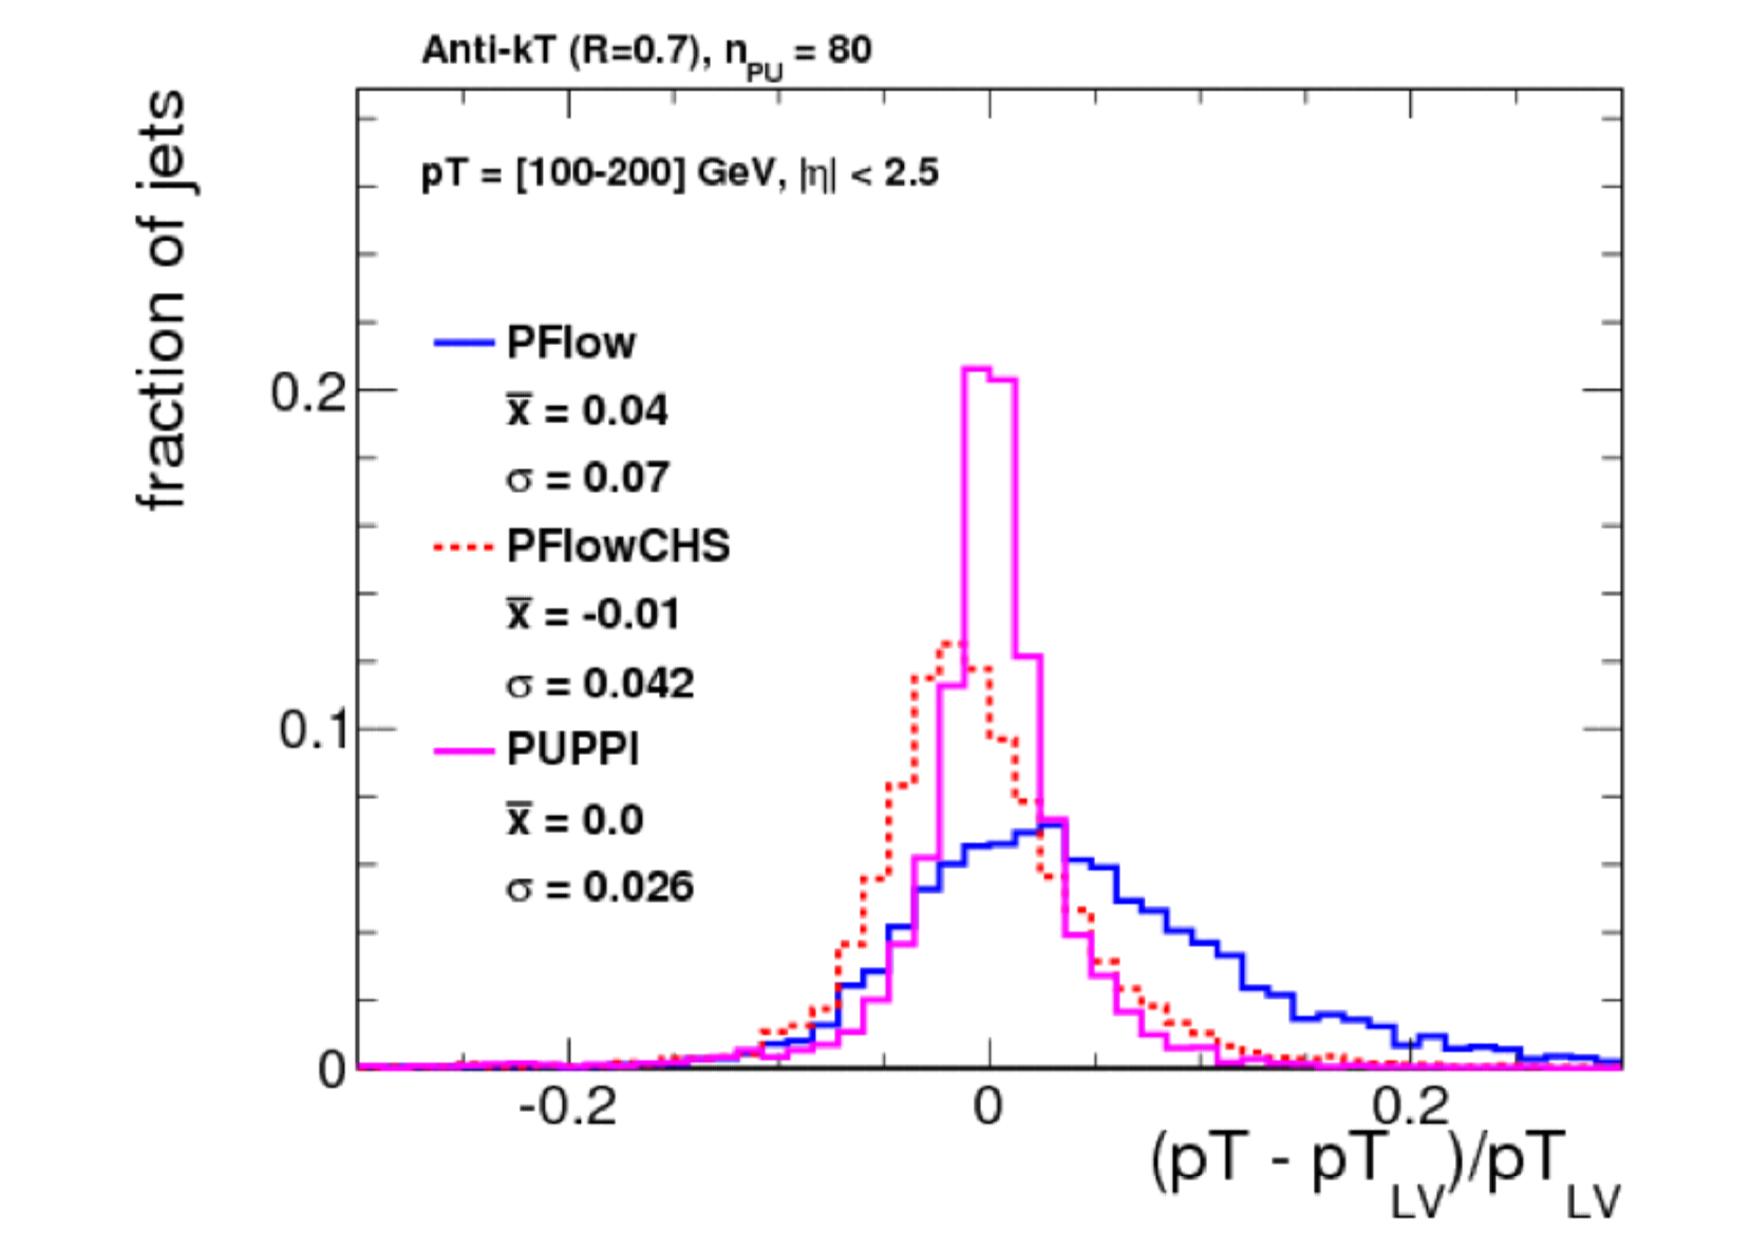
\includegraphics[height=5cm]{figures/event_reconstruction/puppi_ptres_hiPt.pdf}
    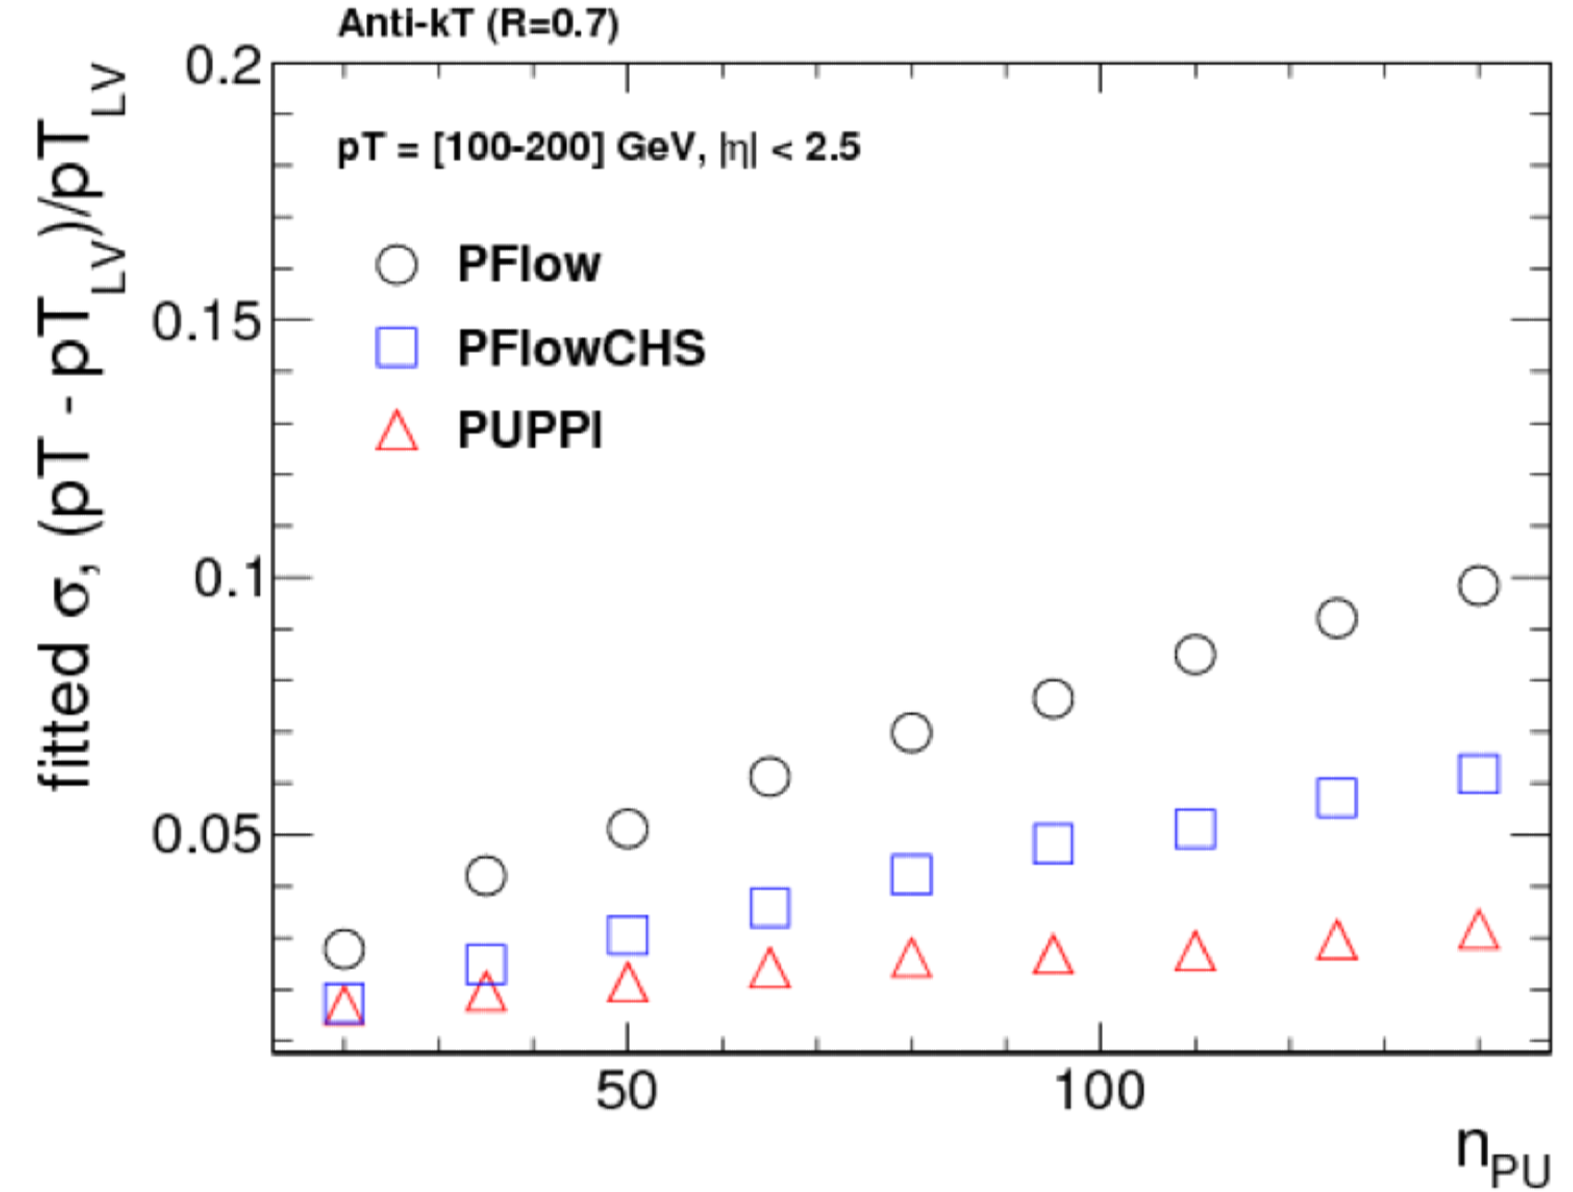
\includegraphics[height=5cm]{figures/event_reconstruction/puppi_ptresVsPu.pdf}
    \caption{The mass (top) and \PT (bottom) resolution comparing PF only (blue), PF+CHS (red) and PUPPI (pink) jets. The absolute resolution (left) as well as the resolution as a function of the number of reconstructed primary vertices in the event (right)is shown~\cite{Bertolini2014}.}
    \label{fig:objreco:puppi}
\end{figure}

The top row shows the absolute mass resolution (left) as well as the mass resolution as a function of $N_{PV}$ for CHS jets (red) and PUPPI (pink) jets. The bottom row shows the corresponding quantities but for jet transverse momentum. A significantly better resolution on jet observables can be achieved using PUPPI compared to CHS.



\section{Jet reconstruction}
As explained in Section~\ref{sec:theory:qcd}, quarks and gluons are never themselves visible in a detector. Within $10^{-23}$ seconds, the timescale of the strong interactions, they fragment and hadronize into a collimated spray of hadrons, a so-called jet. In order to infer the properties of the original parton generating the jet, the properties of the full particle spray needs to be evaluated.
Combining these particles algorithmically is non-trivial, and several algorithms designed to do, called jet clustering algorithms, exist.
These provide a set of rules for grouping particles together into jets and are usually based on certain distance requirements between particles as well as rules for how to recombine their momenta.
Thanks to Particle Flow, objects like charged hadrons, neutral hadrons and photons together with their estimated energy and direction are already defined, and jet clustering in CMS therefore consists of
associating these particles to one common origin.


\subsection{Jet clustering}

The most common jet clustering algorithms used in hadron colliders are the Cambridge/Aachen algorithm~\cite{Dokshitzer:1997in}, the \kt algorithm~\cite{Ellis:1993tq} and the anti-\kt algorithm~\cite{Cacciari:2008gp}. These are all sequential recombination algorithms, meaning they systematically go through each particle pair in the event and recombines them into one particle if the combination satisfies certain criteria. The rules, shared by all three algorithms, are as follows:
\begin{enumerate}
\item For each pair of particles $i$ and $j$, compute the longitudinally invariant distances
  \begin{align}  
  d_{ij} &= \textrm{min}(p_{ti}^{2p},p_{tj}^{2p})\frac{\Delta R^2_{ij}}{R^2} \textrm{, with } \quad \Delta R^2_{ij}&=(\eta_i - \eta_j)^2+(\phi_i - \phi_j)^2\\
  d_{iB} &= p_{ti}^{2p},
  \end{align}  
  where $d_{ij}$ is a measure of the relative transverse momenta between the particles, $\Delta R^2_{ij}$ is the distance between them in the $\eta-\phi$ plane (which can be roughly translated into a jet radius), $\Delta R^2$ corresponds to the configurable desired jet cone size and $d_{iB}$ is the distance between the particle and the beam. The parameter $p$ is what separates the three algorithms from one another and controls the relative power of energy versus geometrical
scales. For the anti-\kt algorithm, it is defined as $p=-1$, for the \kt algorithm $p=1$ and in the case of the C/A algorithm, $p=0$. The consequences of these choices are explained in detail below.
  \item Find the minimum distance of $d_{ij}$ and $d_{iB}$.
  \item If this is $d_{ij}$, recombine particles $i$ and $j$ and return to step 1.
  \item If it is $d_{iB}$, the particle is $i$is defined to be a final state jet, and is removed from the list of particles. The algorithms proceeds back to step 1.
  \item Repeat until no particles remain.
\end{enumerate}

\subsubsection{Infrared and collinear safety}
There are two requirements that are extremely important when defining jet algorithms: They must be 1) \textit{infrared} (IR) and 2) \textit{collinear} (C) safe.
\textit{Infrared} safety corresponds to the requirement that if the final state particles are modified by the presence of a soft emission, and there are always soft emission in QCD events (both perturbative and non-perturbative), then the set of hard jets should remain unchanged. This is illustrated by the two left figures in Figure~\ref{fig:objreco:IRC}.

\begin{figure}[ht] 
    \centering
    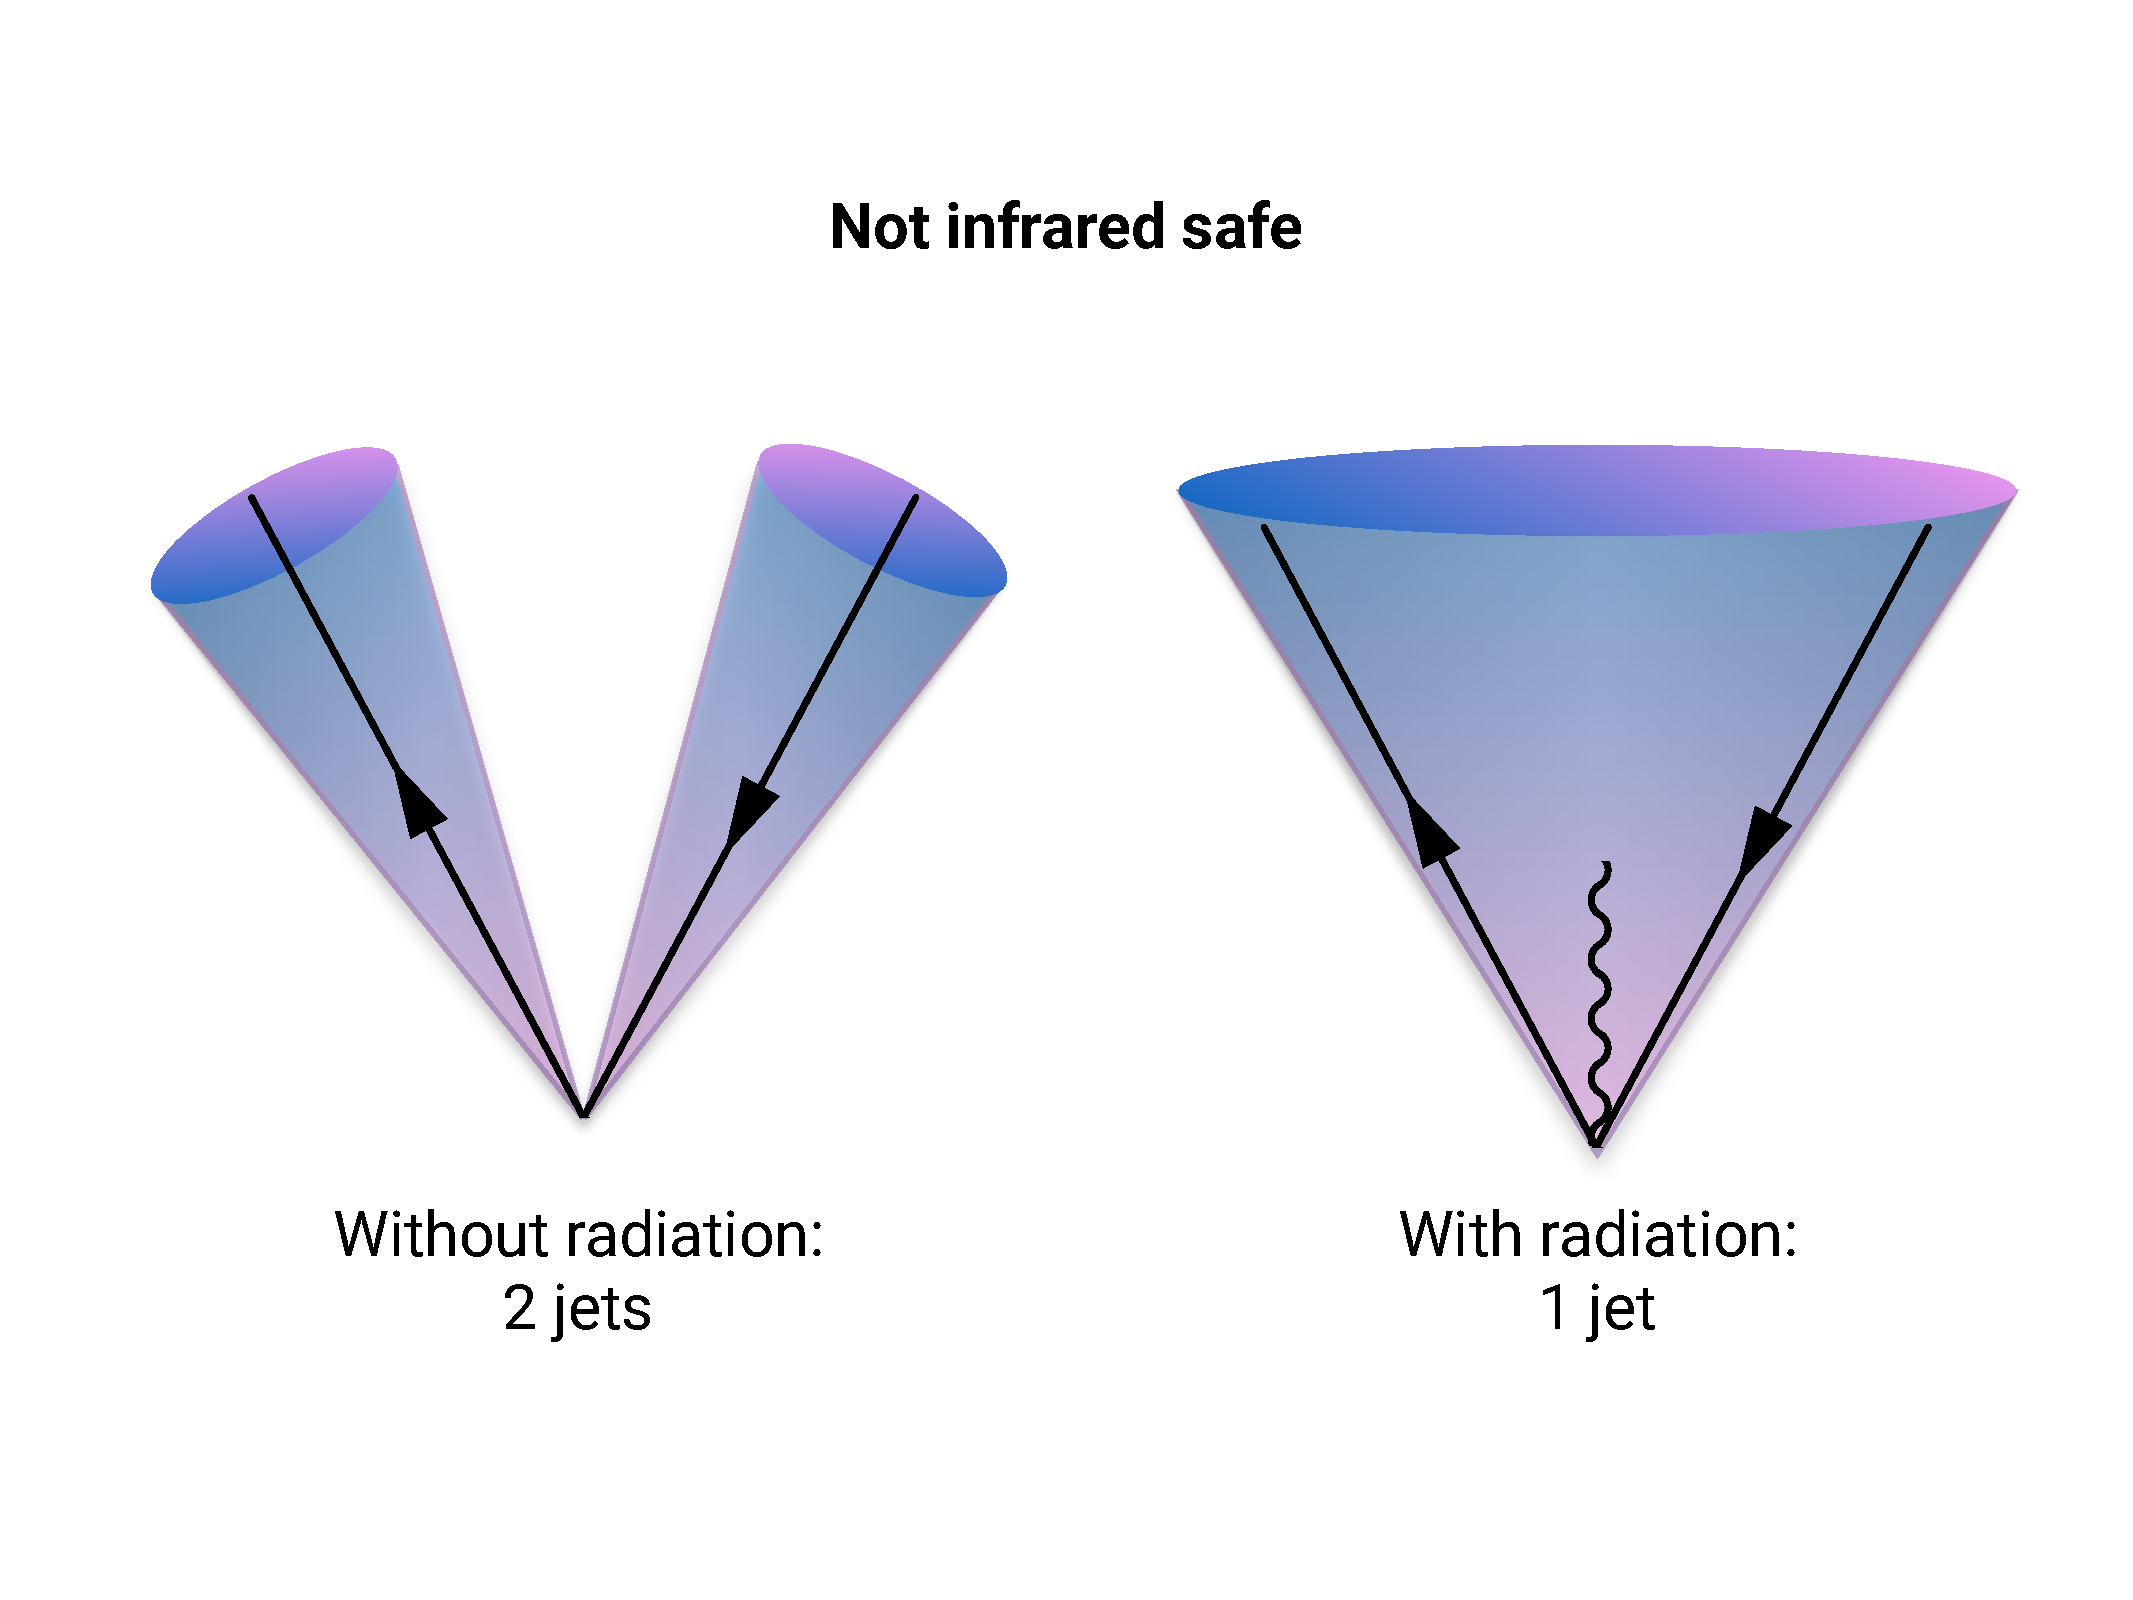
\includegraphics[width=0.49\textwidth]{figures/event_reconstruction/IR_safety.pdf}
    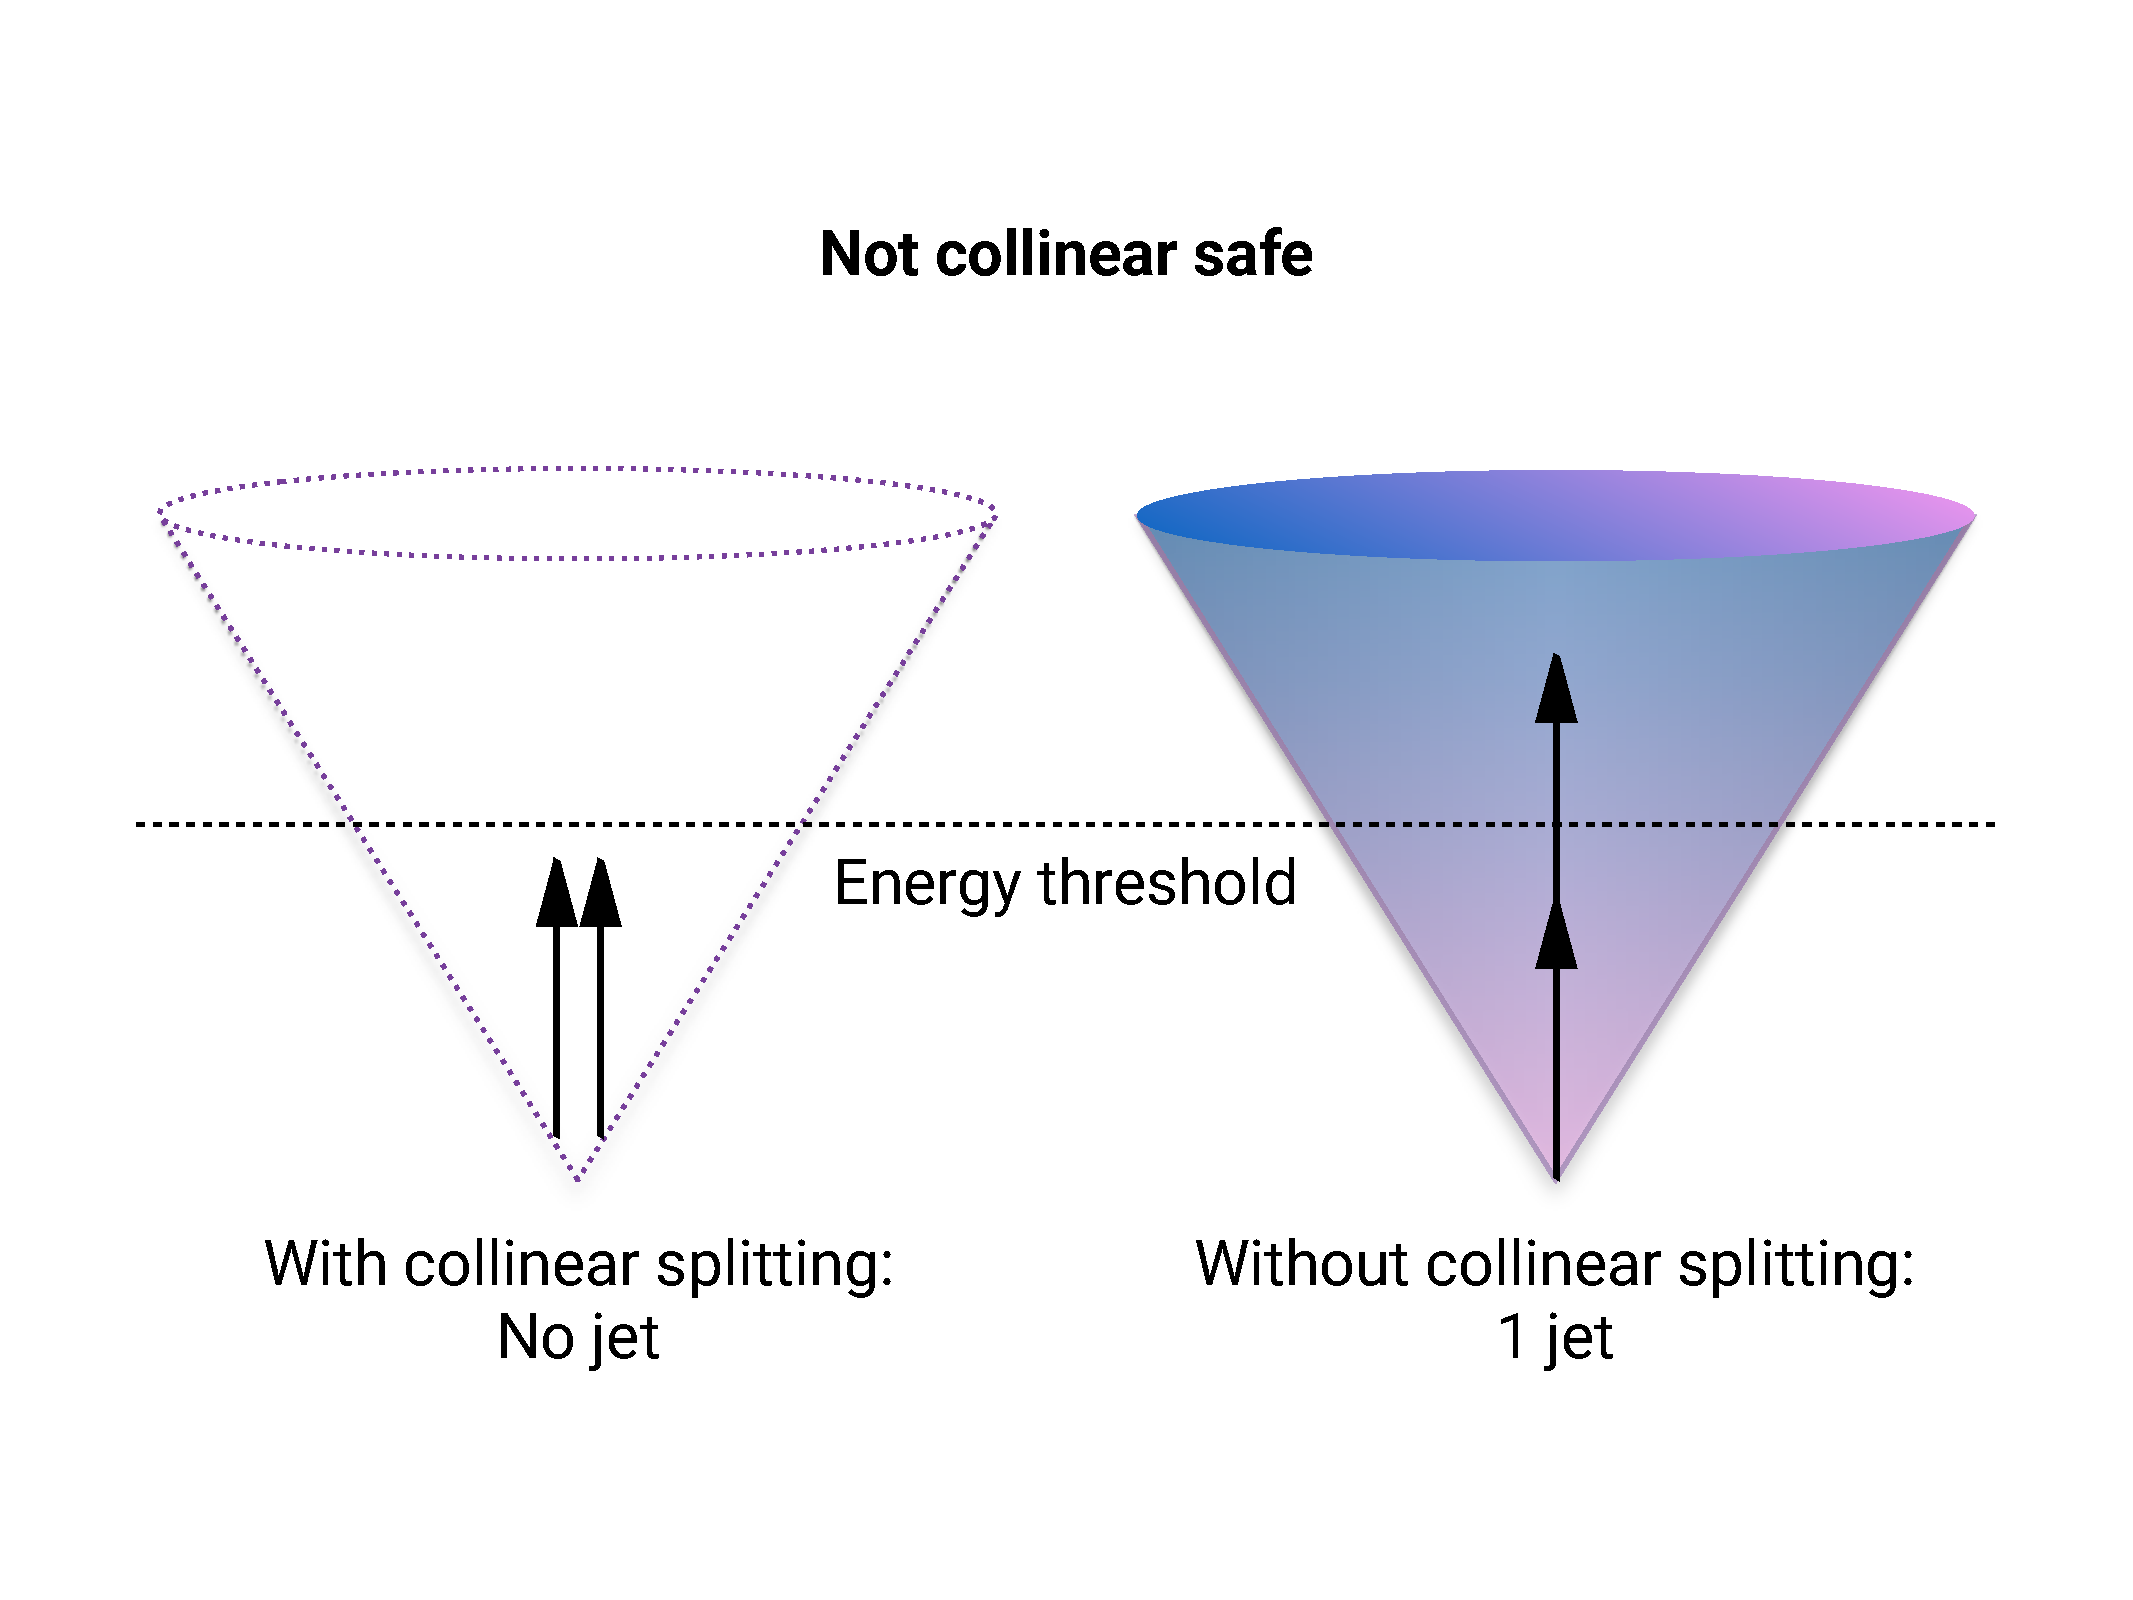
\includegraphics[width=0.49\textwidth]{figures/event_reconstruction/Collinear_safety.pdf}
    \caption{An illustration of what would happen for an infrared (left) and collinear (right) unsafe jet algorithm. If an algorithm is infrared unsafe, the presence of a soft emission changes the jet configuration. If an algorithm is collinear unsafe, then if a parton undergoes a collinear splitting this will change the configuration of the jet}
    \label{fig:objreco:IRC}
\end{figure}

Here, the algorithm is infrared unsafe: the presence of an additional soft gluon changes the jet configuration from 2 to 1 jets. If an algorithm is \textit{collinear} unsafe, it means that the jet configuration would change if the hard parton undergoes collinear splitting (which a hard parton often does as part of the fragmentation process and which are also part of non-perturbative dynamics, like the decay of highly energetic hadrons). This is shown in the two left figures of Figure~\ref{fig:objreco:IRC}, where a hard parton undergoing collinear splitting fails to be reconstructed due to its daughters being below the energy threshold of the algorithm.


All sequential recombination algorithms are trivially infrared safe.
 
\subsubsection{The \kt algorithm}
The \kt algorithm is the oldest of the sequential recombination algorithms and, due to its $p=1$ definition in the distance measures, follows the QCD branching structure in both \PT and in angle (in reverse). Soft particles are clustered together first, and the final step is the clustering of the two hardest particles. A consequence of this definition is that there is nothing that keeps arbitrarily soft particles from being defined as jets, and a minimum cut on the jet \PT should be introduced.
Despite several favorable qualities, the \kt algorithm is not the algorithm of choice in most hadron collider experiments due to the irregular jets it produces, a consequence of clustering soft particles first.

\subsubsection{The Cambridge/Aachen algorithm}
The Cambridge/Aachen algorithm, with $p=0$ in the distance measures, follows the QCD branching structure only in angle as the clustering order is based solely on spatial separation. The simplest of the algorithms, it recombines all pairs close in $\Delta R$ until $\Delta R_{ij} > R$.
The benefits of this is that the clustering history contains information about the presence of any geometrical substructure within a jet, a feature that will become important in Section~\ref{sec:objreco:substructure}.

\subsubsection{The anti-\kt algorithm}
The default jet clustering algorithm in CMS is the anti-\kt algorithm~\cite{Cacciari:2008gp}, which follows the rules and distance measures above with $p=-1$. The algorithm favors the clustering of high-\PT - high-\PT and high-\PT – low-\PT particles first, disfavoring clustering between soft particles. That means the algorithm grows around a hard core, yielding jets with a well-defined cone shaped area. Together with being IRC-safe and insensitive to the underlying event (any event not arising the primary hard scattering process) and pileup, makes it the main jet algorithm in CMS.



A comparison of the resulting jet area in the $\phi-\eta$ plane after clustering with either \kt, C/A and anti-\kt, is shown in Figure~\ref{fig:objreco:jetalgo_comp}. The z-axis correspond to the parton \PT. One can clearly see that when clustering with the anti-\kt algorithm, the produced jets are circular, with a radius set by $R$, around the hardest parton.

\begin{figure}[ht] 
    \centering
    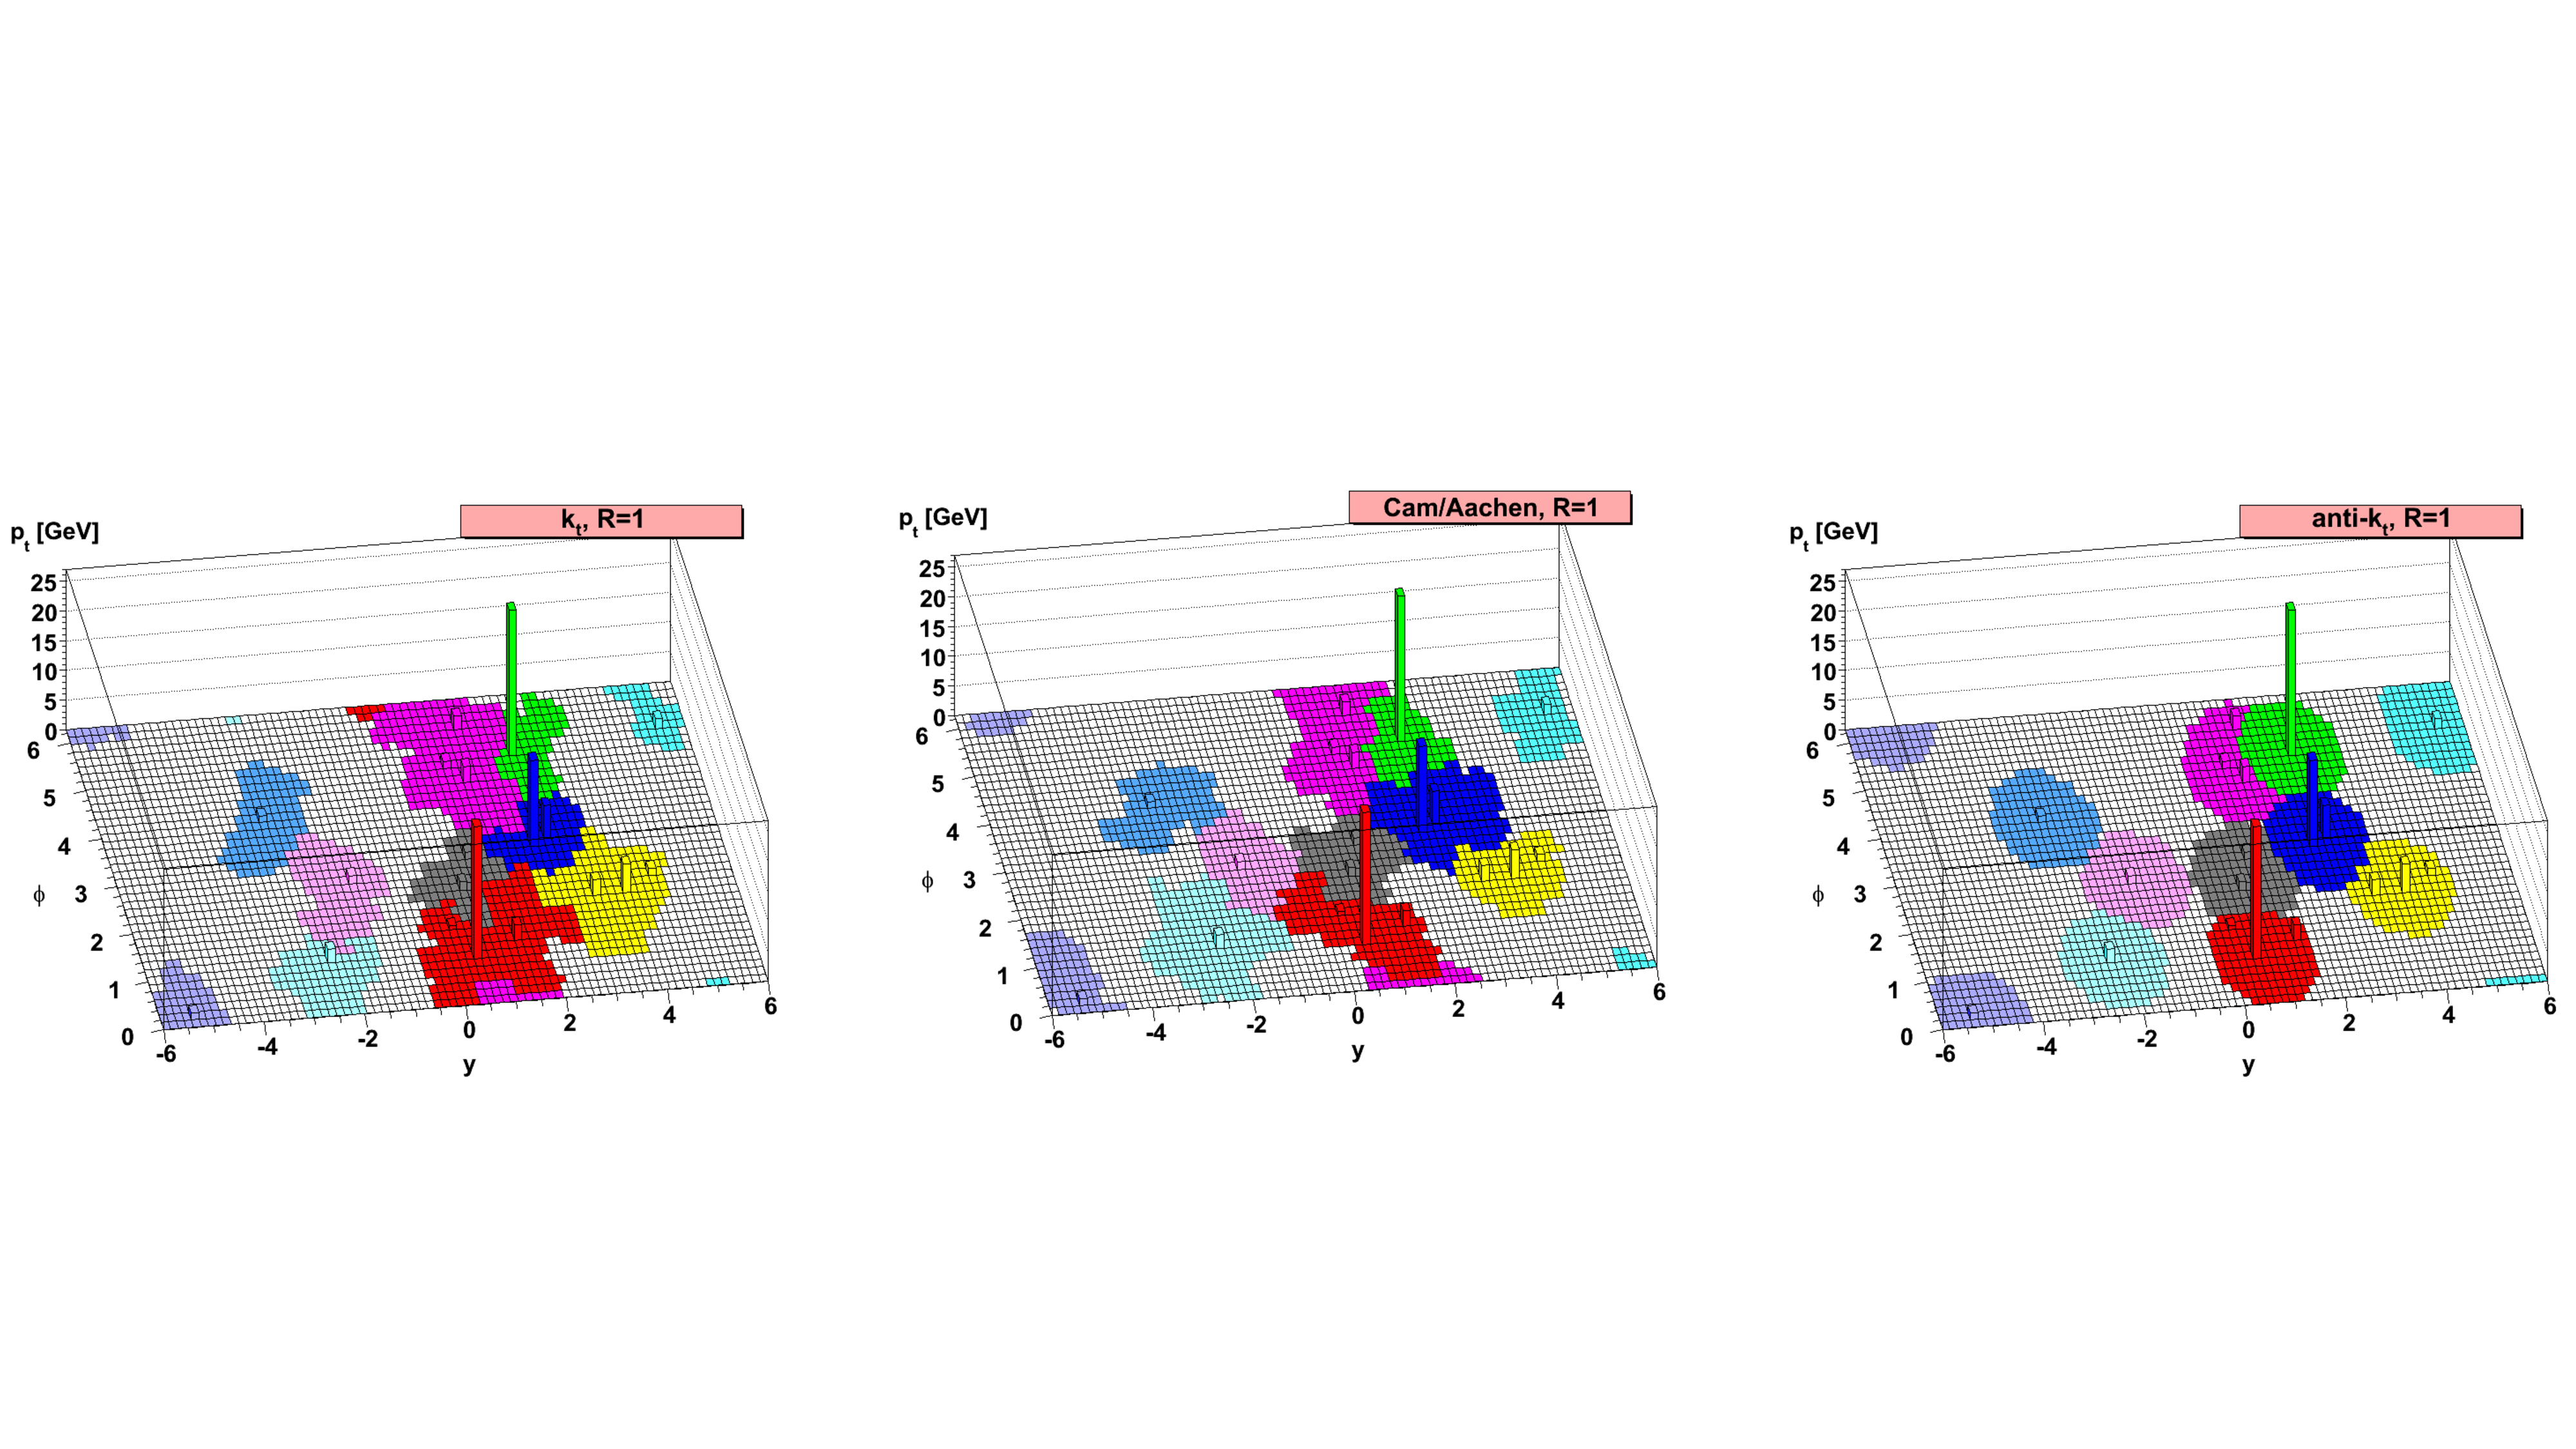
\includegraphics[width=0.99\textwidth]{figures/event_reconstruction/clustering_algos.pdf}
    \caption{A comparison of the resulting jet cone area in the $\phi-\eta-\PT$ plane after clustering the same event with three different jet algorithms: \kt, C/A and anti-\kt. ~\cite{Cacciari:2008gp}}
    \label{fig:objreco:jetalgo_comp}
\end{figure}

\subsubsection{Particle Flow, anti-\kt and pileup subtraction }
Jet algorithms in CMS mainly uses PF candidate four-vectors as input and, before clustering occurs, a pileup removal algorithm is usually applied. If using CHS (Section~\ref{subsub:objreco:chs}), charged hadrons not associated to the primary vertex are discarded before clustering. If PUPPI is used (Section~\ref{subsub:objreco:puppi}), all the PF candidates are reweighted based on how likely they are to have originated from pileup. 
CMS by default uses two jet cone sizes: R=0.4 and R=0.8. Jets with R=0.4, called PFAK4, are used for single-prong jets while the larger R=0.8 jets, PFAK8, are more often used when looking for jets containing multiple hard quarks/gluons in order to contain all the hadronization products.

\section{Jet substructure reconstruction}
\label{sec:objreco:substructure}
In analyses looking for highly energetic ("boosted") vector bosons like, a main theme of this thesis, the opening angle between the vector boson quark decay products become so small that the highly boosted boson appears as a single large jet instead of two well-separated smaller jets. The distance between the two quarks, in the case of an hadronic decay, depends on the mass of the vector boson and its \PT and goes as

\begin{equation}  
\Delta R = \frac{2 M_{V}}{p_{T,V}}.  
\end{equation}

Above a W boson \PT of 200 GeV, the two quarks are therefore merged into a single large cone jet of size R = 0.8. A sketch of the two different situation is shown below. If the W \PT is well below 200 GeV, its decay products are well-defined jets in their own right as shown in Figure~\ref{fig:objreco:unmerged}. However, once the W transverse momenta starts exceeding 200 GeV, both the quarks are completely contained within a single jet as is illustrated in Figure~\ref{fig:objreco:merged}.
   
\begin{figure}[ht] 
    \centering
    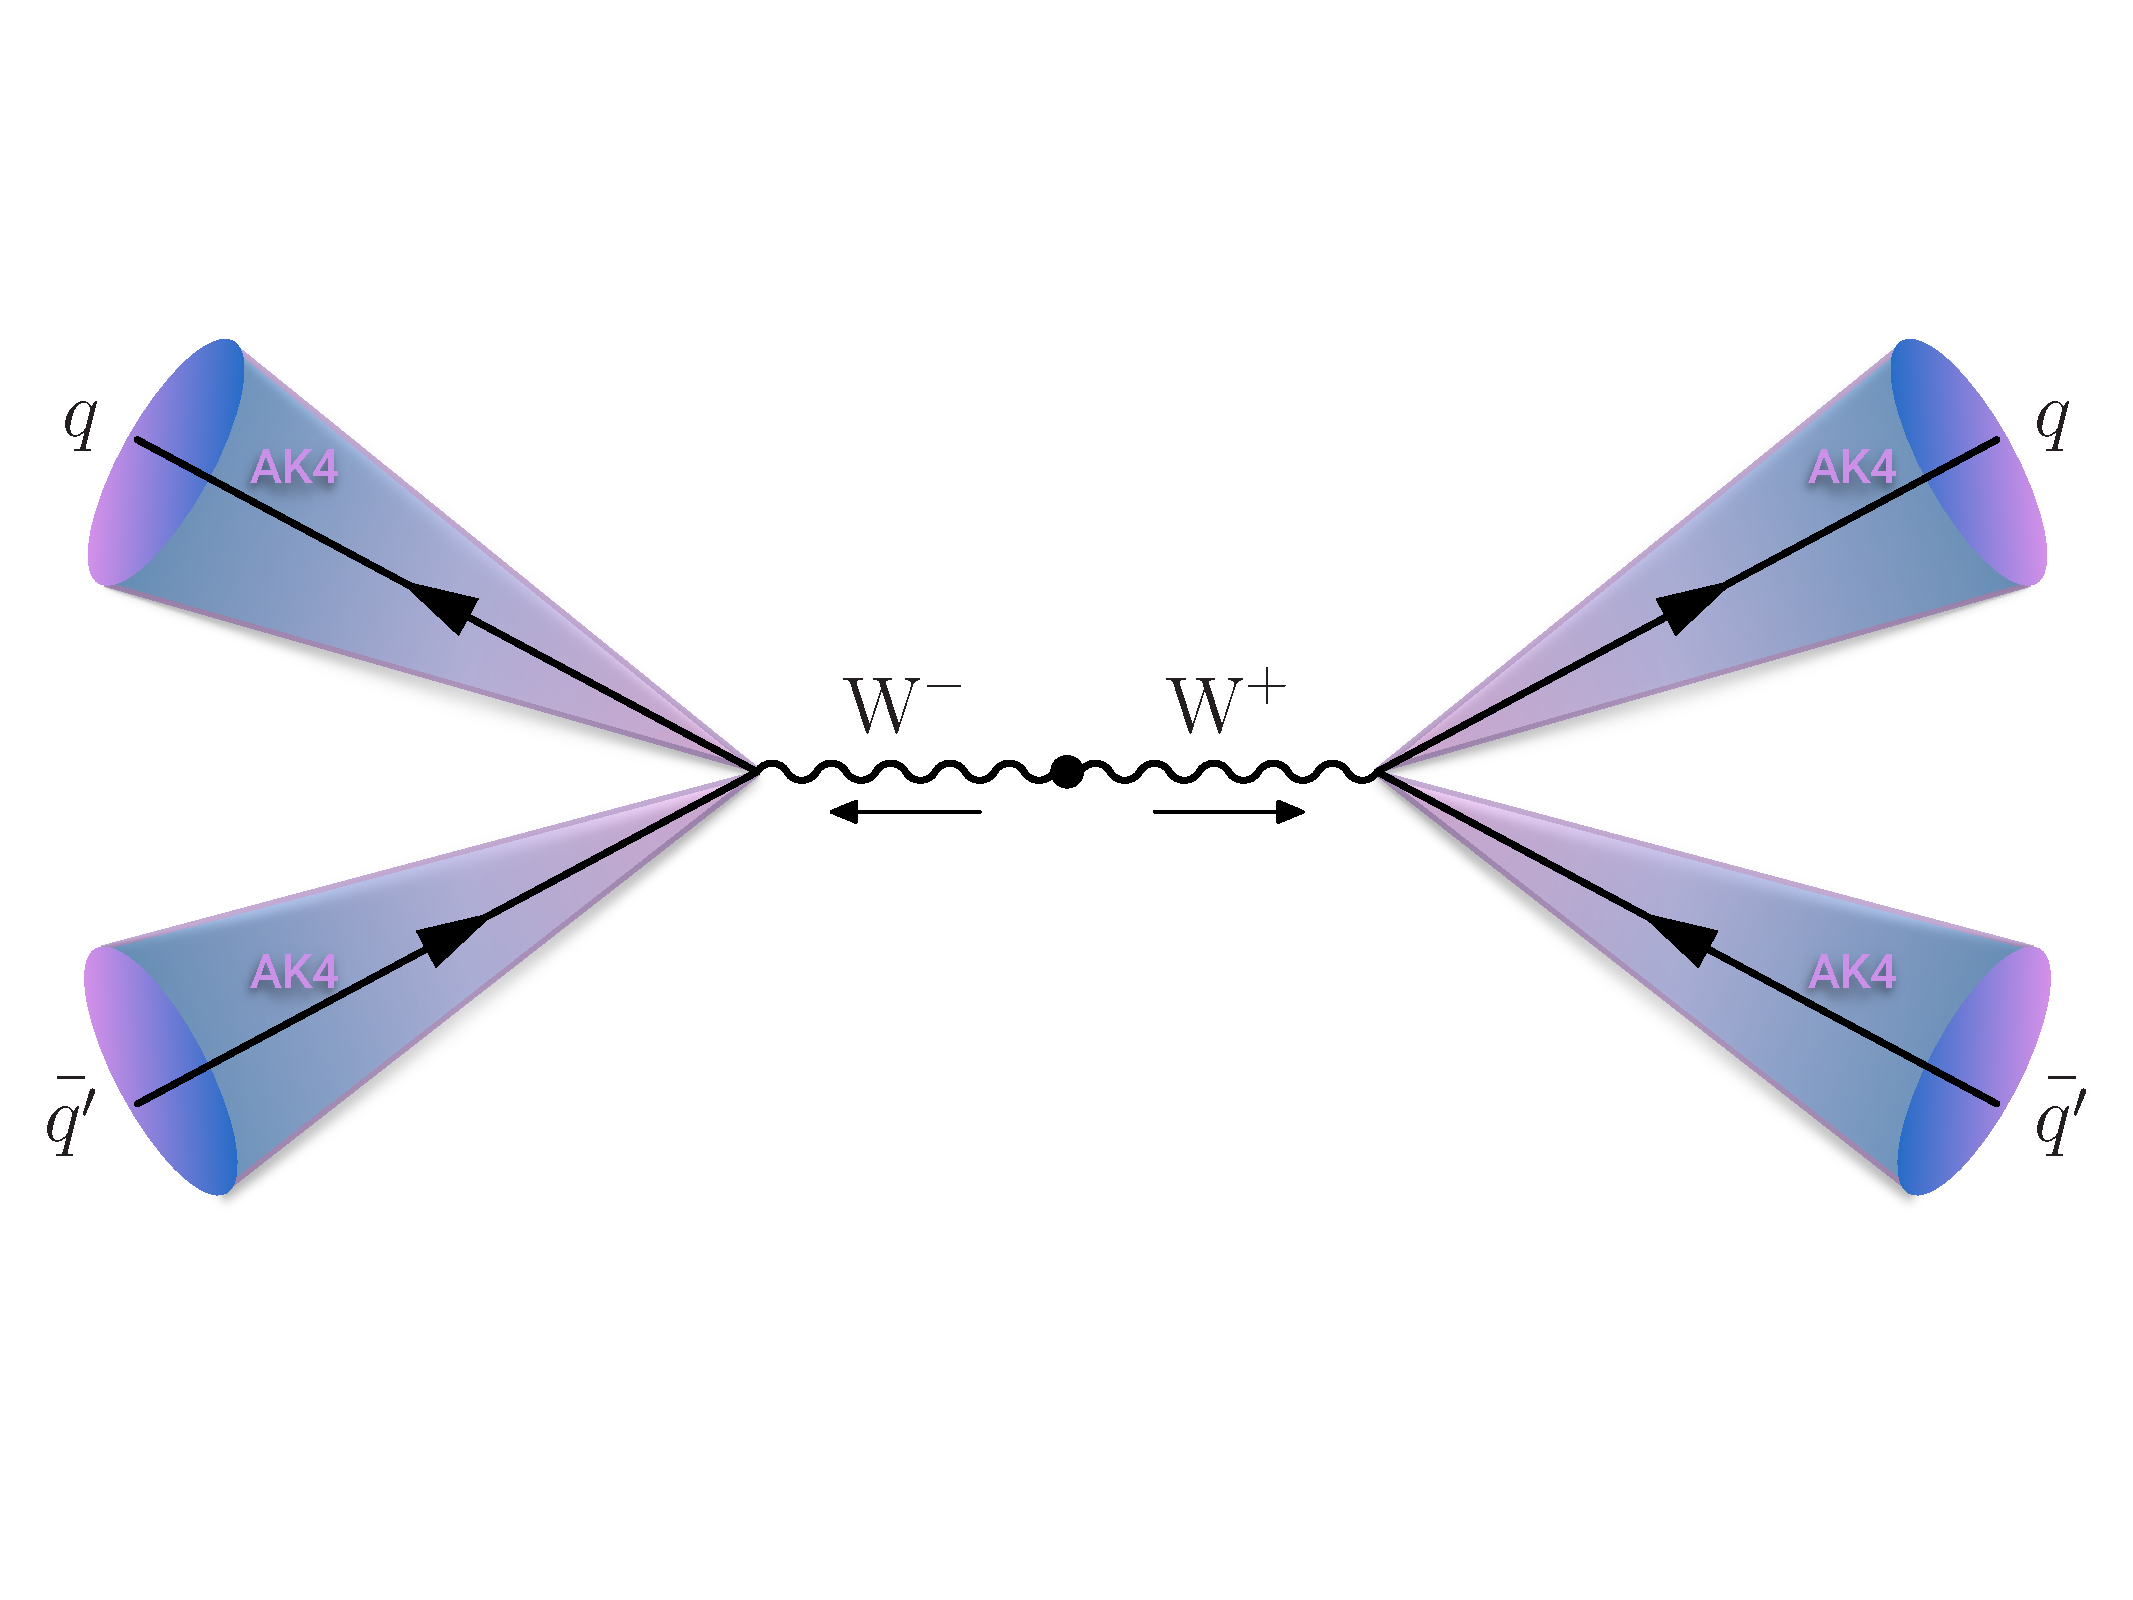
\includegraphics[width=0.70\textwidth]{figures/event_reconstruction/WWqqqq_unmerged_small.pdf}\\
    \caption{If the mass of the resonance is low enough, the quark decay products of each vector boson are well separated and clustered into distinguishable AK4 jets.}
    \label{fig:objreco:unmerged}
\end{figure}

\begin{figure}[ht] 
    \centering
    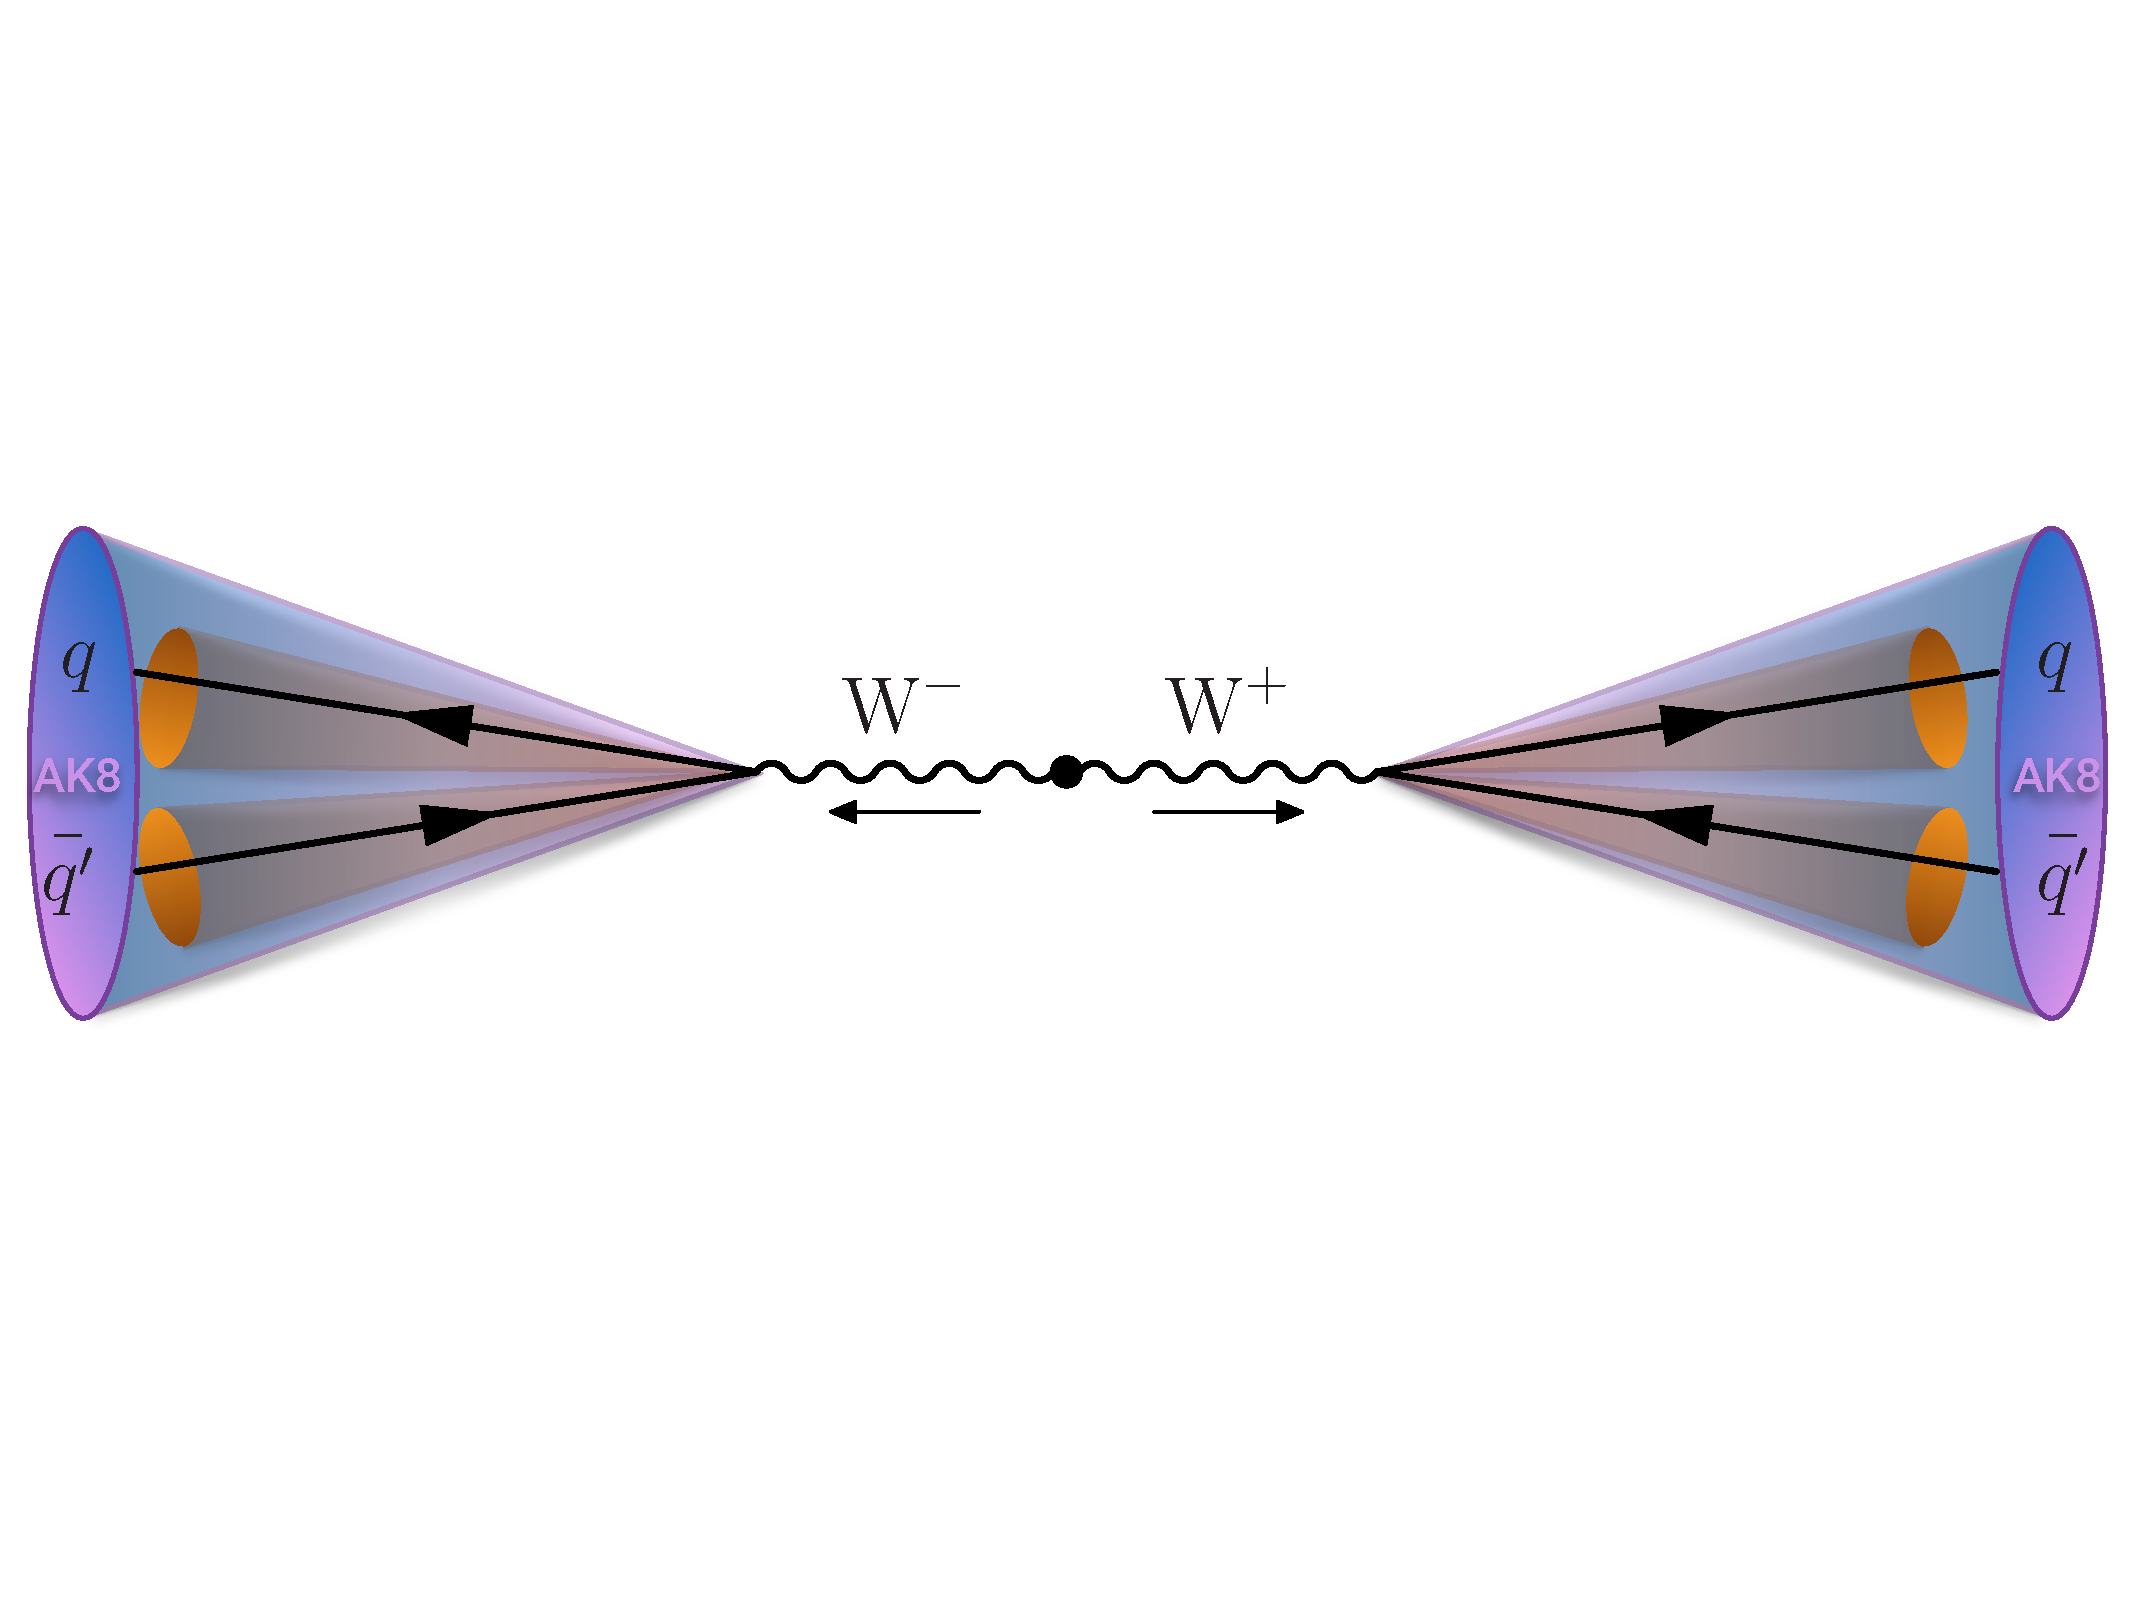
\includegraphics[width=0.70\textwidth]{figures/event_reconstruction/WWqqqq_merged_small.pdf}
    \caption{If the transverse momentum of the vector boson is greater than 200 GeV, the vector boson decay products are merged into one single large cone AK8 jet.}
    \label{fig:objreco:merged}
\end{figure}

In order to distinguish hadronically decaying vector boson from QCD quark/gluon jets, the jet mass would in principle be a good discriminant as we know the W has a mass of around 80 GeV while the quark/gluon mass is close to ~zero. At very high transverse momenta, however, the width (and therefore the mass) of QCD jets may become equally large. In addition, diffuse radiation caused by the Underlying Event and pileup give rise to a significant number of additional particles in the event contributing to the total jet mass.
Therefore, being able to accurately and efficiently separate highly boosted QCD jets from highly boosted vector bosons, requires other methods.
In order to get red of UE and pileup, algorithms like PUPPI and CHS can be used. Then, to improve the mass resolution further, dedicated grooming algorithms must be applied.

\subsection{Grooming}
Grooming was introduces as a tool to improve the signal, most often \PW/\PZ/, mass resolution without significantly changing the background and signal event numbers. It consists of removing the softest parts of a jet in order to resolve its "true" mass, by means of reclustering and identifying soft particles within the jet which then are removed.

\subsubsection{Trimming}
The trimming algorithm~\cite{Krohn:2009th} is a grooming algorithm mostly used at trigger level in CMS (also where it is used in this thesis) due to it being less aggressive than other grooming algorithms. It works in the following way: Starting from a large jet clustered with either anti-\kt or C/A (in the case of CMS), it reclusters the jet using the \kt algorithm in order to create subjets of some size $R_{sub}$.  It then proceeds to check whether each subjet has a momentum fraction above a certain threshold,
\begin{equation*}
p_{T,i}/p_{T,jet}>p_{T,frac}.
\end{equation*}
If the subjet fails this requirement, it is removed. The remaining subjets are then assembled into a new "trimmed" jet.
The effect of trimming on real W jets and QCD quark/gluon jets for different values of $r_{sub}$ and $p_{T,frac}$ is shown in Figure~\ref{fig:objreco:trimming}. 
The best signal mass resolution is obtained with $r_{sub}=0.2$ and $p_{T,frac}=0.03$, which is also the parameter setting that provides the best signal and background 
discrimination by pushing the QCD jet mass closer to zero. These are the default values of the tuned parameters of the trimming algorithm in CMS ($r_{sub}=0.2$ and $p_{T,frac}=0.03$).

\begin{figure}[ht] 
    \centering 
    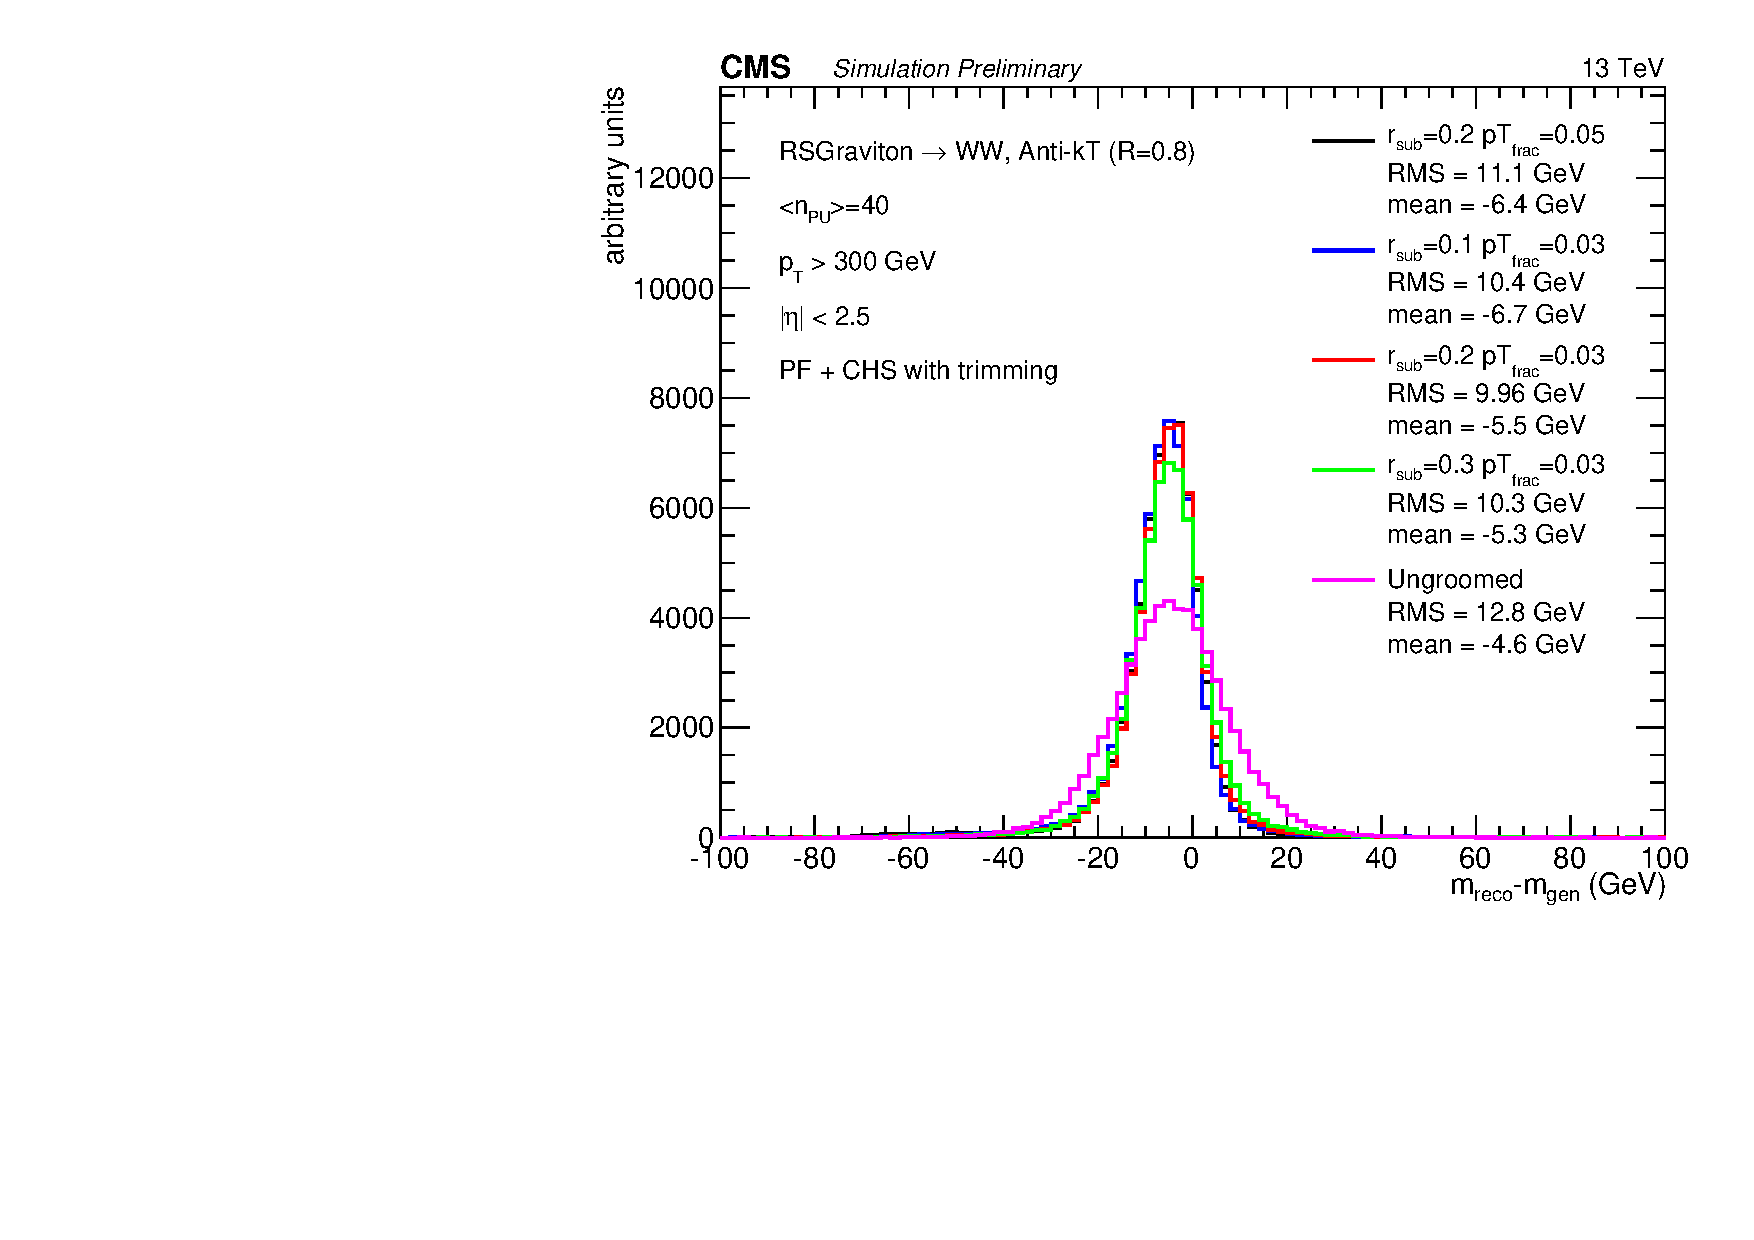
\includegraphics[height=6cm]{figures/event_reconstruction/sig_trimming.pdf}
    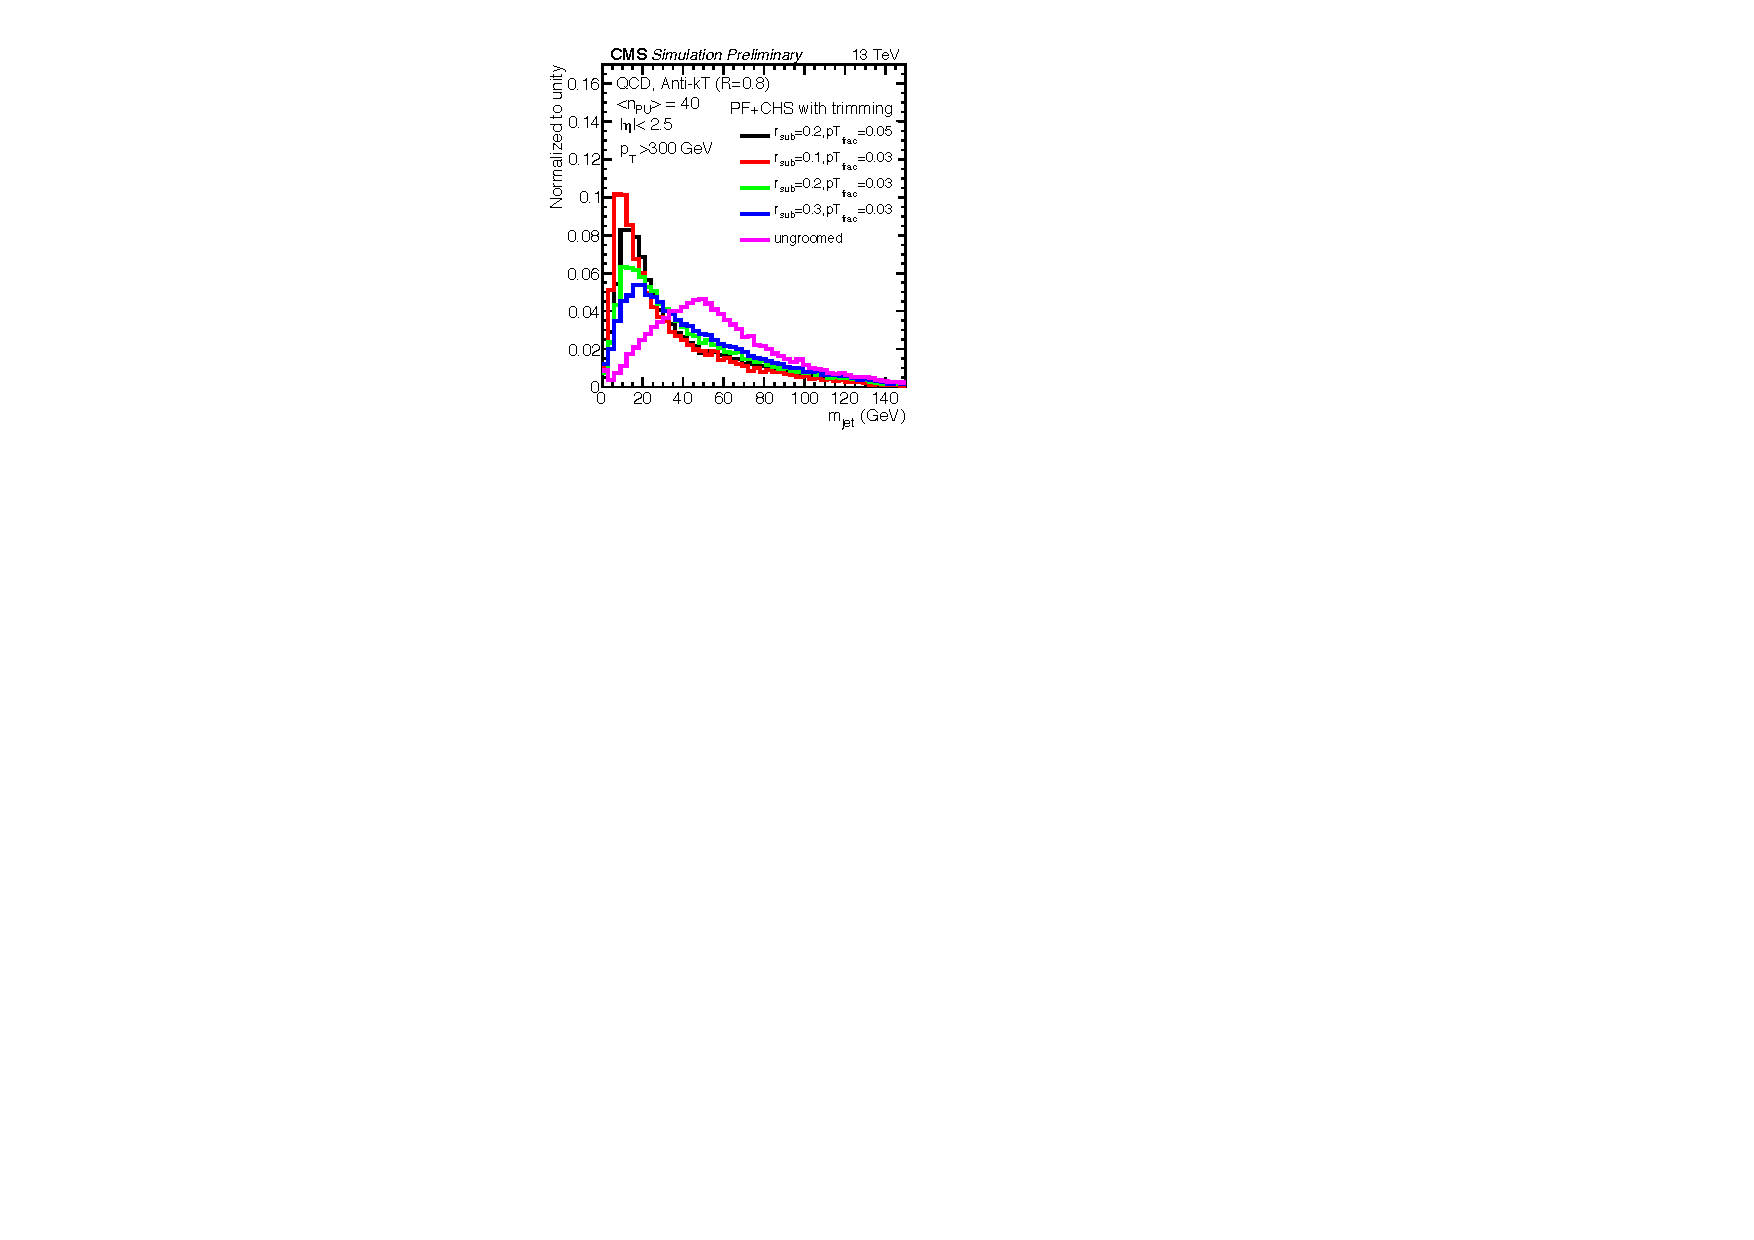
\includegraphics[height=6cm]{figures/event_reconstruction/bkg_trimming-noData.pdf}
    \caption{The effect of trimming on a signal jet (left) and a background jet (right) for different values of the tuned parameters $r_{sub}$ and $p_{T,frac}$~\cite{CMS-PAS-JME-14-001}.}
    \label{fig:objreco:trimming}
\end{figure}

\subsubsection{Pruning}
The pruning algorithm, in addition to removing soft particles, has an additional requirement on the distance between any recombination that are at wide angle.
It proceeds by reclustering the jet with the C/A algorithm, requiring at each step that

\begin{equation*}
\frac{ \textrm{min}(p_{T,i},p_{T,j}) }{ p_{T,P} } > z_{cut} \quad \textrm{ and } \quad \Delta R_{i,j} < D_{cut} = \frac{2 r_{cut} m_{jet}}{\PT}.
\end{equation*}

The first requirement is a requirement on the hardness of the combination. $p_{T,i}$ and $,p_{T,j}$ correspond to the transverse momenta of each protojet (single particle or group of particles already combined in a previous step) and $p_{T,P}$ is the combined \PT of the two. The protojet with the lowest transverse momenta is removed if its hardness is below $z_{cut}$, or if it forms an angle wider than $D_{cut}$ relative to the axis of the recombination of the two protojets. In CMS, the tuned parameters are set to $r_{cut}=0.5$ and where $z_{cut}=0.1$. Figure~\ref{fig:objreco:pruning} shows the ungroomed as well as the pruned jet mass distribution for signal (left) and background jets. The highest amount of signal and background separation in CMS, is achieved with $r_{cut}=0.5$ and $z_{cut}=0.1$.

\begin{figure}[ht] 
    \centering
    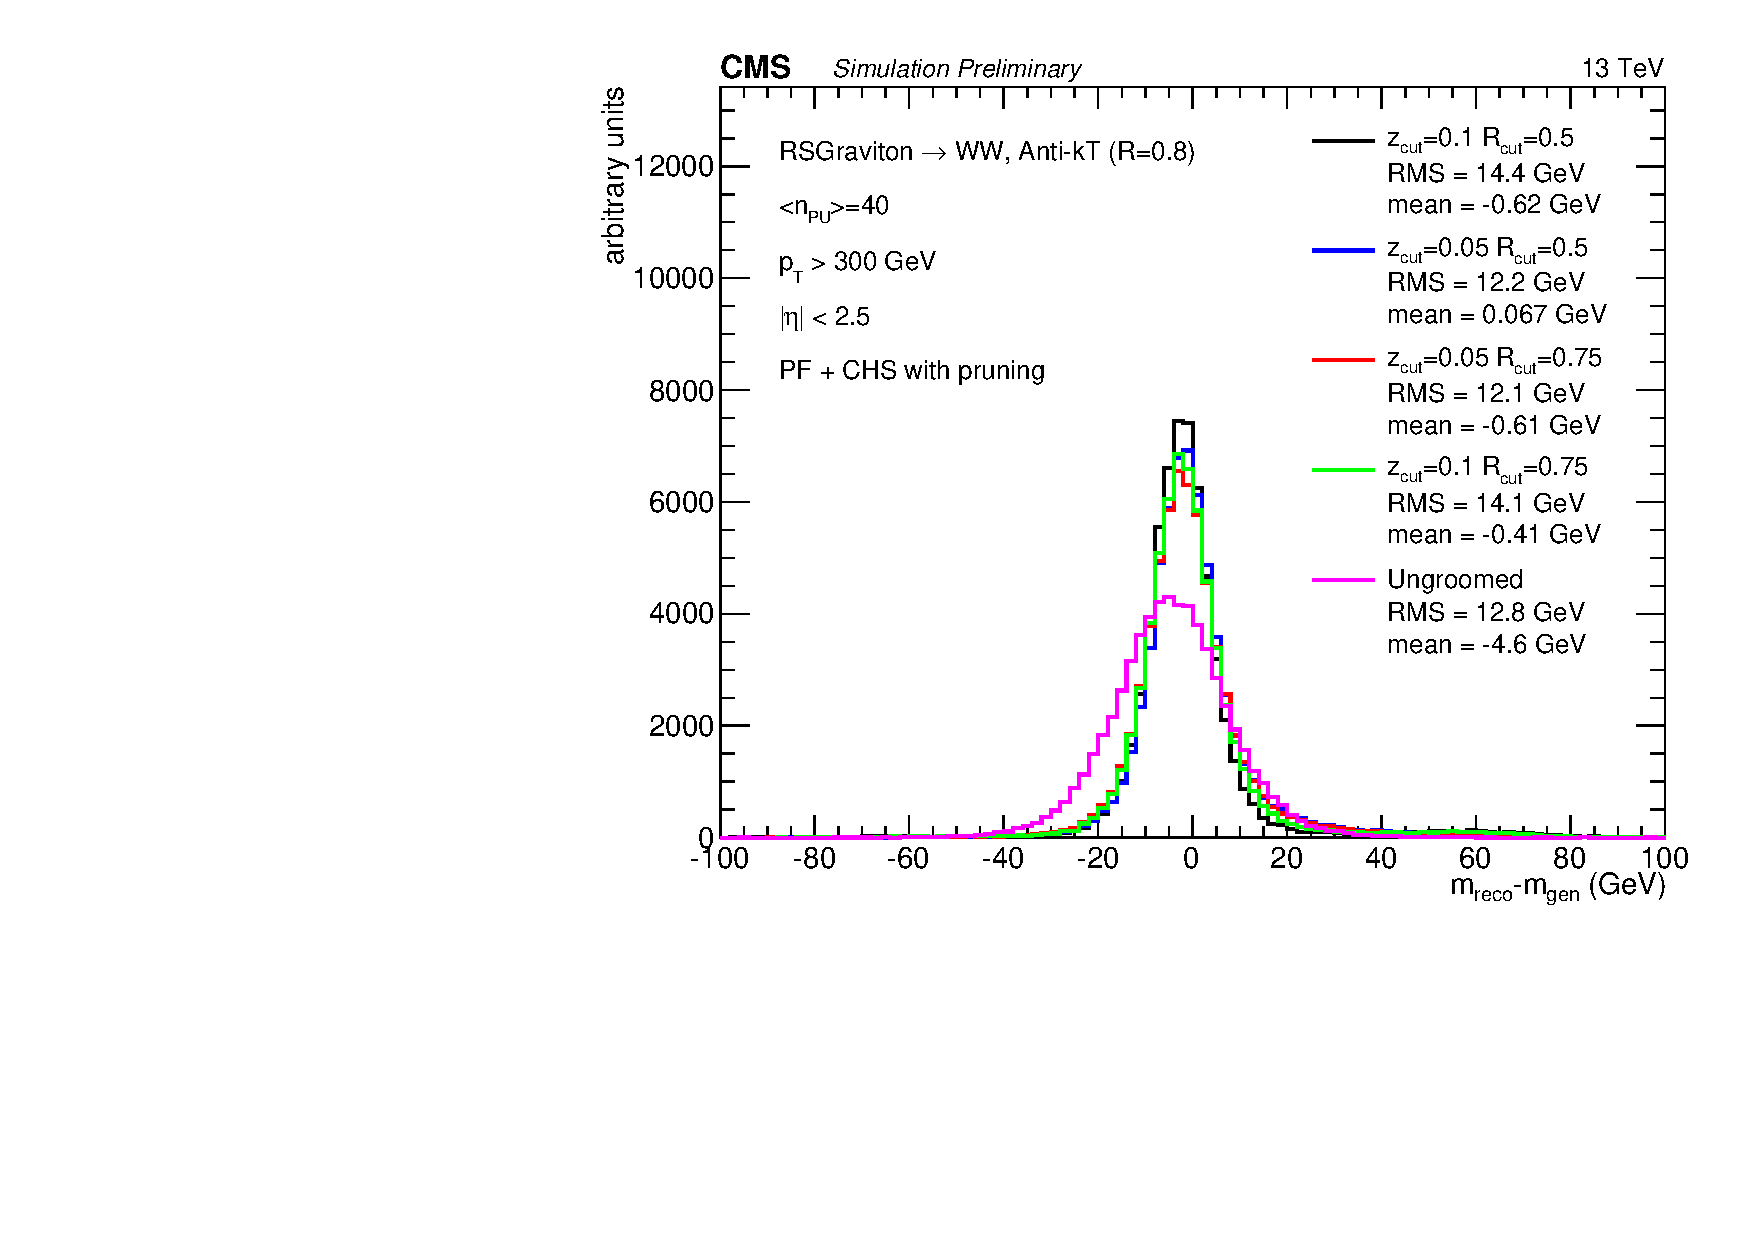
\includegraphics[height=6cm]{figures/event_reconstruction/sig_pruning.pdf}
    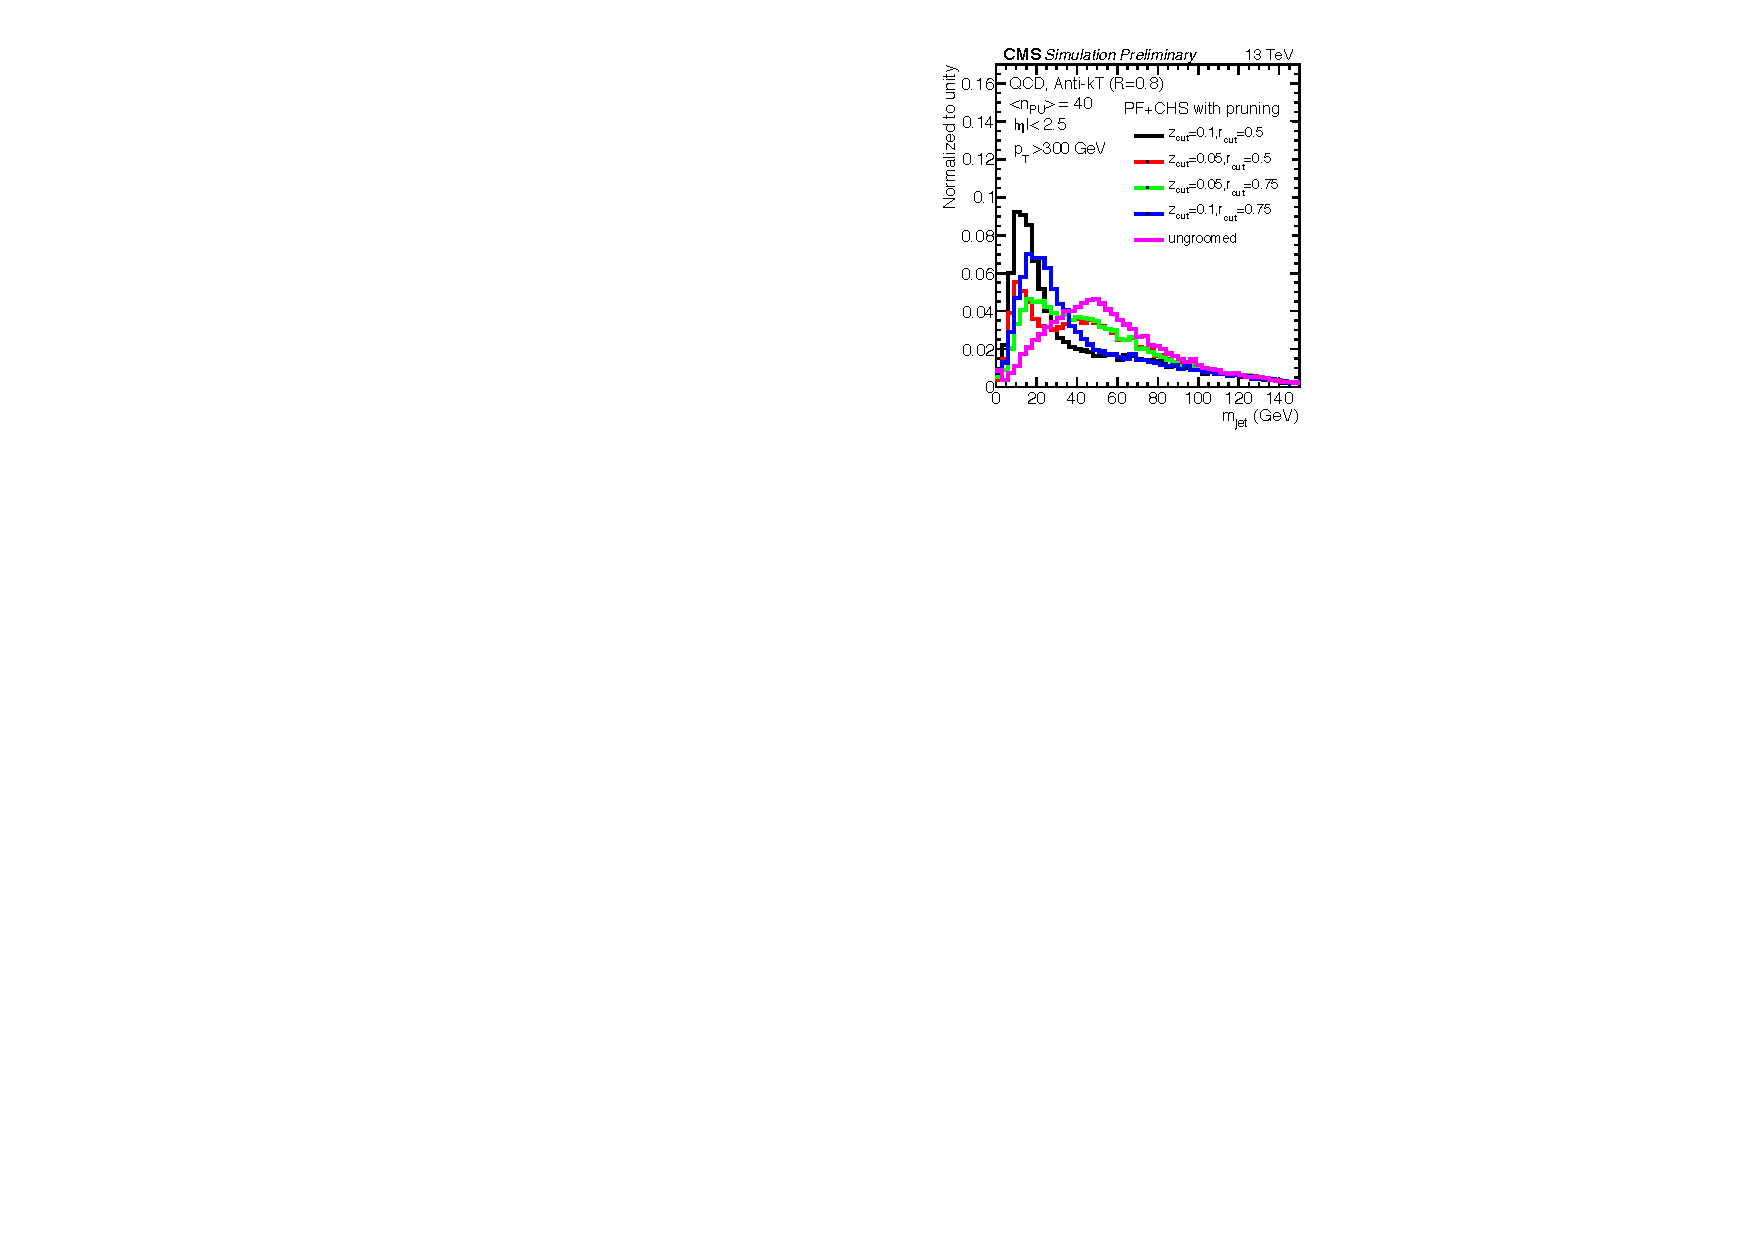
\includegraphics[height=6cm]{figures/event_reconstruction/bkg_pruning-noData.pdf}
    \caption{The effect of pruning on a signal jet (left) and a background jet (right) for different values of the tuned parameters $z_{cut}$ and $r_{cut}$~\cite{CMS-PAS-JME-14-001}.}
    \label{fig:objreco:pruning}
\end{figure}



\subsubsection{Modified Mass Drop Tagger and Soft Drop}

The modified mass drop tagger (mMDT)~\cite{Dasgupta:2013ihk} (a modified version of the originally suggested mass drop tagger ~\cite{Butterworth:2008iy}) is based on the idea that a \PW/\PZ jet is formed by two quark subjets and that, therefore, the mass of each subjet is much smaller than their combined mass (and much smaller than the mass of the boson itself). A QCD jet is, on the other hand, formed by continuous soft radiation, meaning that its heaviest subjet should be close to the mass of the jet itself. The mMDT tagger therefore starts from an already clustered jet, reclusters it with the C/A algorithm and then declusters it again defining subjets $s_1$ and $s_2$. It then looks for a significant mass drop going from total jet mass to the mass of each subjet, and checks that the splitting is not too asymmetric. The modified mass drop condition is generalized through the soft drop declustering method~\cite{Larkoski:2014wba}, simply called Soft Drop, which allows for different types of angular requirements to enter the condition. The Soft Drop condition is the following

\begin{equation*}
\frac{ \textrm{min}(p_{T,1},p_{T,2}) }{ p_{T,1}+p_{T,2} } > z_{cut} \frac{\Delta R_{12}}{R_0}^\beta.
\end{equation*}

If no significant mass drop occurred and the splitting is not to asymmetric, the condition is met and the full jet is deemed the softdrop jet. Otherwise only the highest-\PT subjet is kept and the declustering continues. If the jet can not be declustered any further, it can either be removed from consideration, so-called "tagging"-mode, or deemed the final soft-dropped jet, "grooming"-mode. A $\beta=0$ corresponds to the modified mass drop tagger and removes all soft emission from the jet. For $\beta>0$, soft radiation is removed, but some fraction of soft-collinear radiation is kept. Lastly, with $\beta<0$, Soft Drop can remove soft as well as collinear radiation.
The performance of Soft Drop on W jets and QCD quark/gluon jets for different values of $\beta$ is shown in Figure~\ref{fig:objreco:softdrop}. The modified mass drop tagger (Softdrop with $\beta$=0) is the default Soft Drop settings in CMS, due to it providing the best signal/background discrimination while maintaining an excellent signal mass resolution.


\begin{figure}[ht] 
    \centering 
    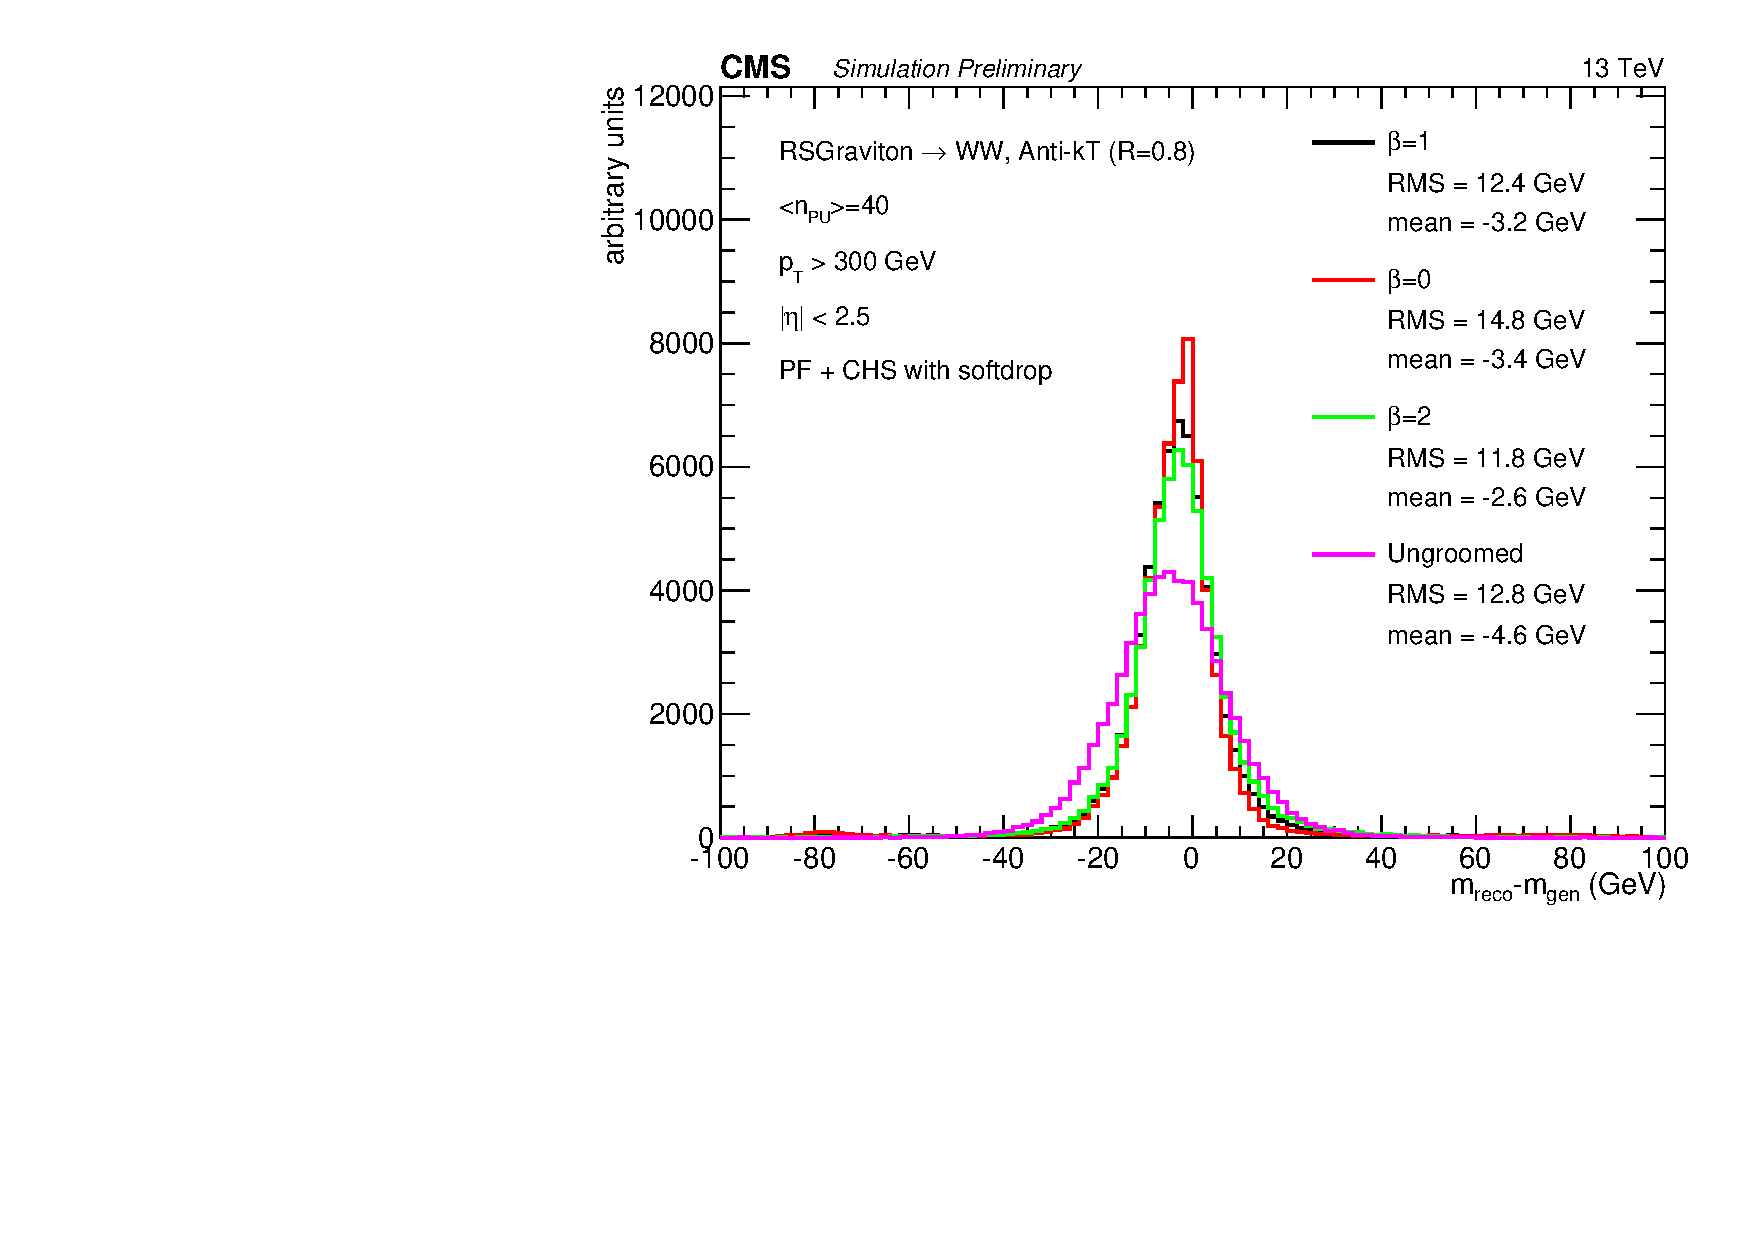
\includegraphics[height=6cm]{figures/event_reconstruction/sig_sd.pdf}
    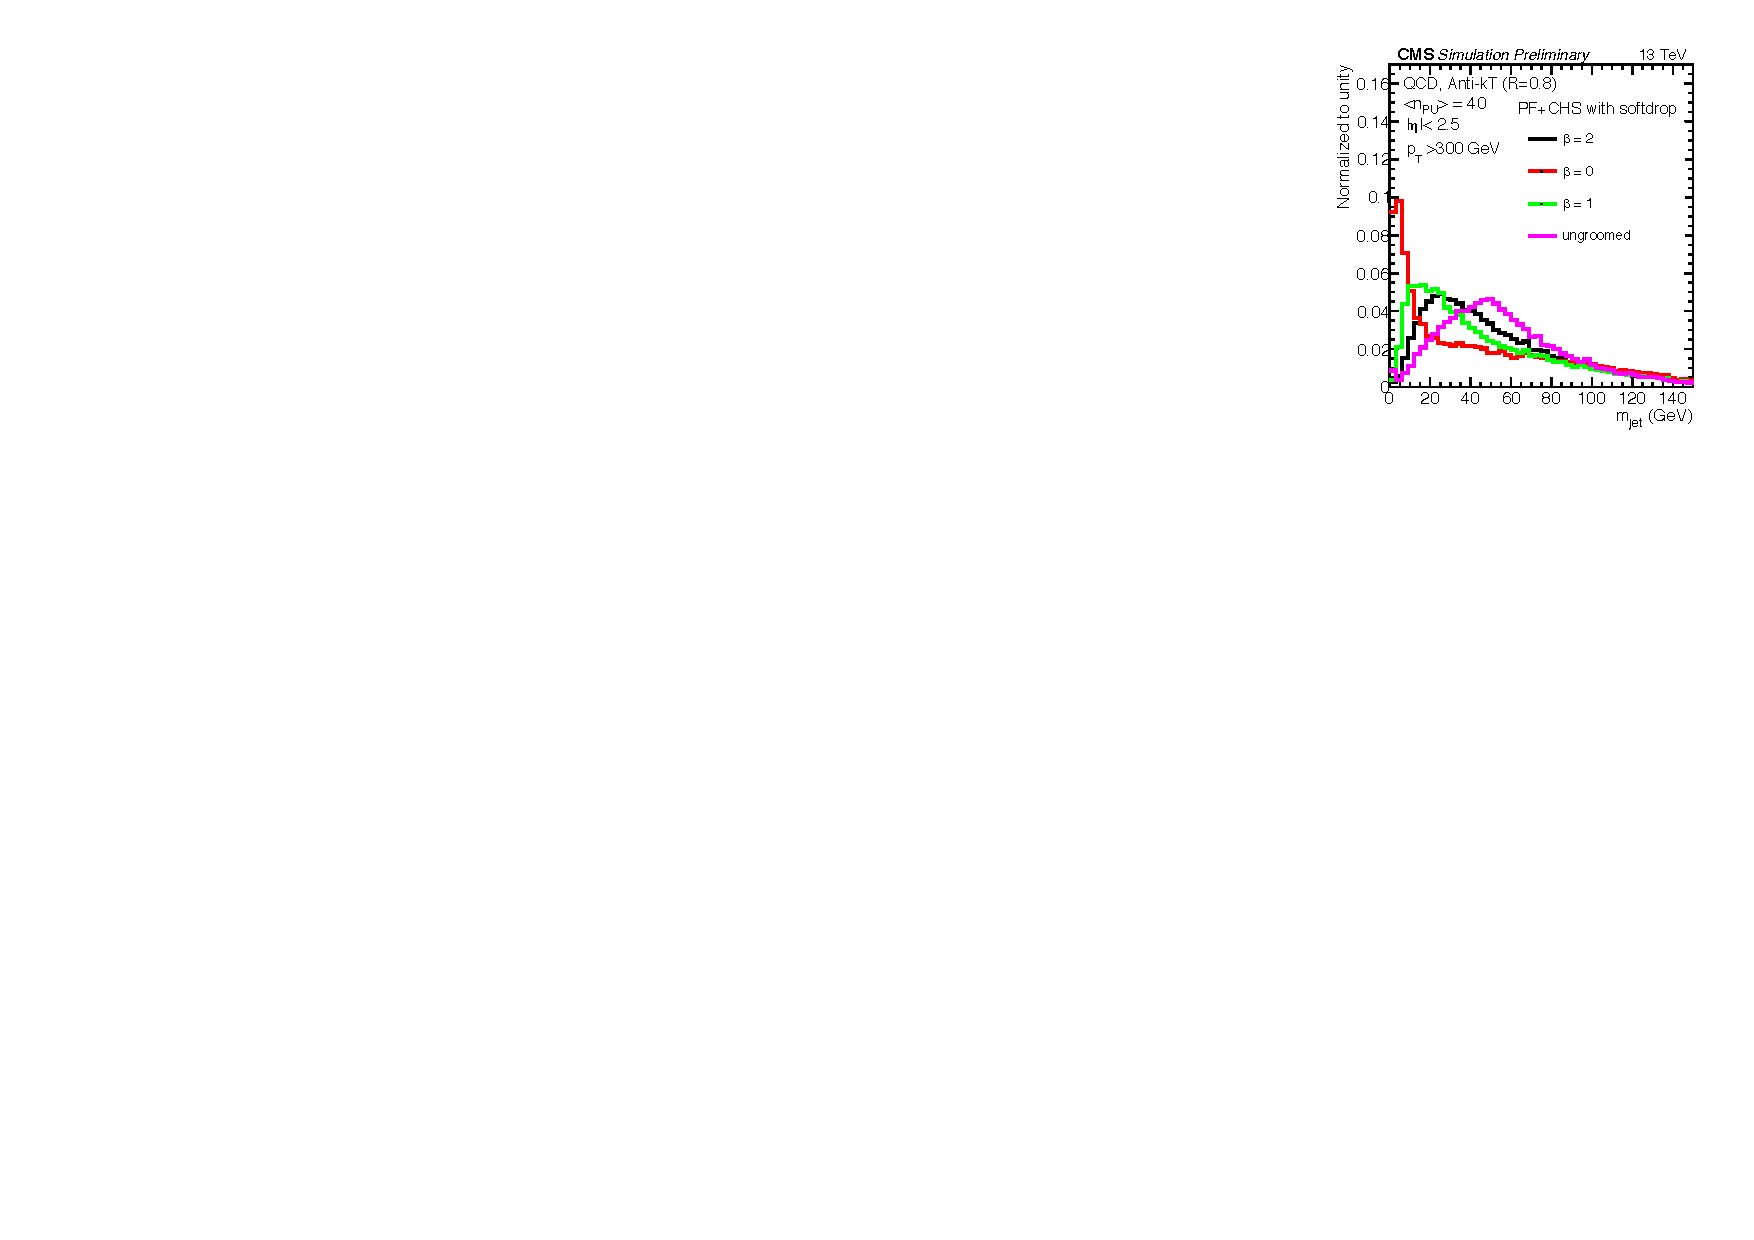
\includegraphics[height=6cm]{figures/event_reconstruction/bkg_softdrop-noData.pdf}
     \caption{The effect of softdrop on a signal jet (left) and a background jet (right) for different values of the tuned parameters $\beta$. $\beta=0$ corresponds to the Modified Mass Drop Tagger, which is the default Softdrop setting in CMS ~\cite{CMS-PAS-JME-14-001}.}
     \label{fig:objreco:softdrop}
 \end{figure}

\subsection{N-subjettiness}
After hopefully having resolved the particle mass with one of the grooming algorithms above, there is still discriminating information to be gathered from the jet structure itself.
A \PW or \PZ jet consists of two well-defined high-\PT subjets. A quark/gluon jet on the other hand, made from a single parton, consists of several large angle, asymmetric splittings, as illustrated in Figure~\ref{fig:objreco:onevstwoprong}

\begin{figure}[ht] 
    \centering 
    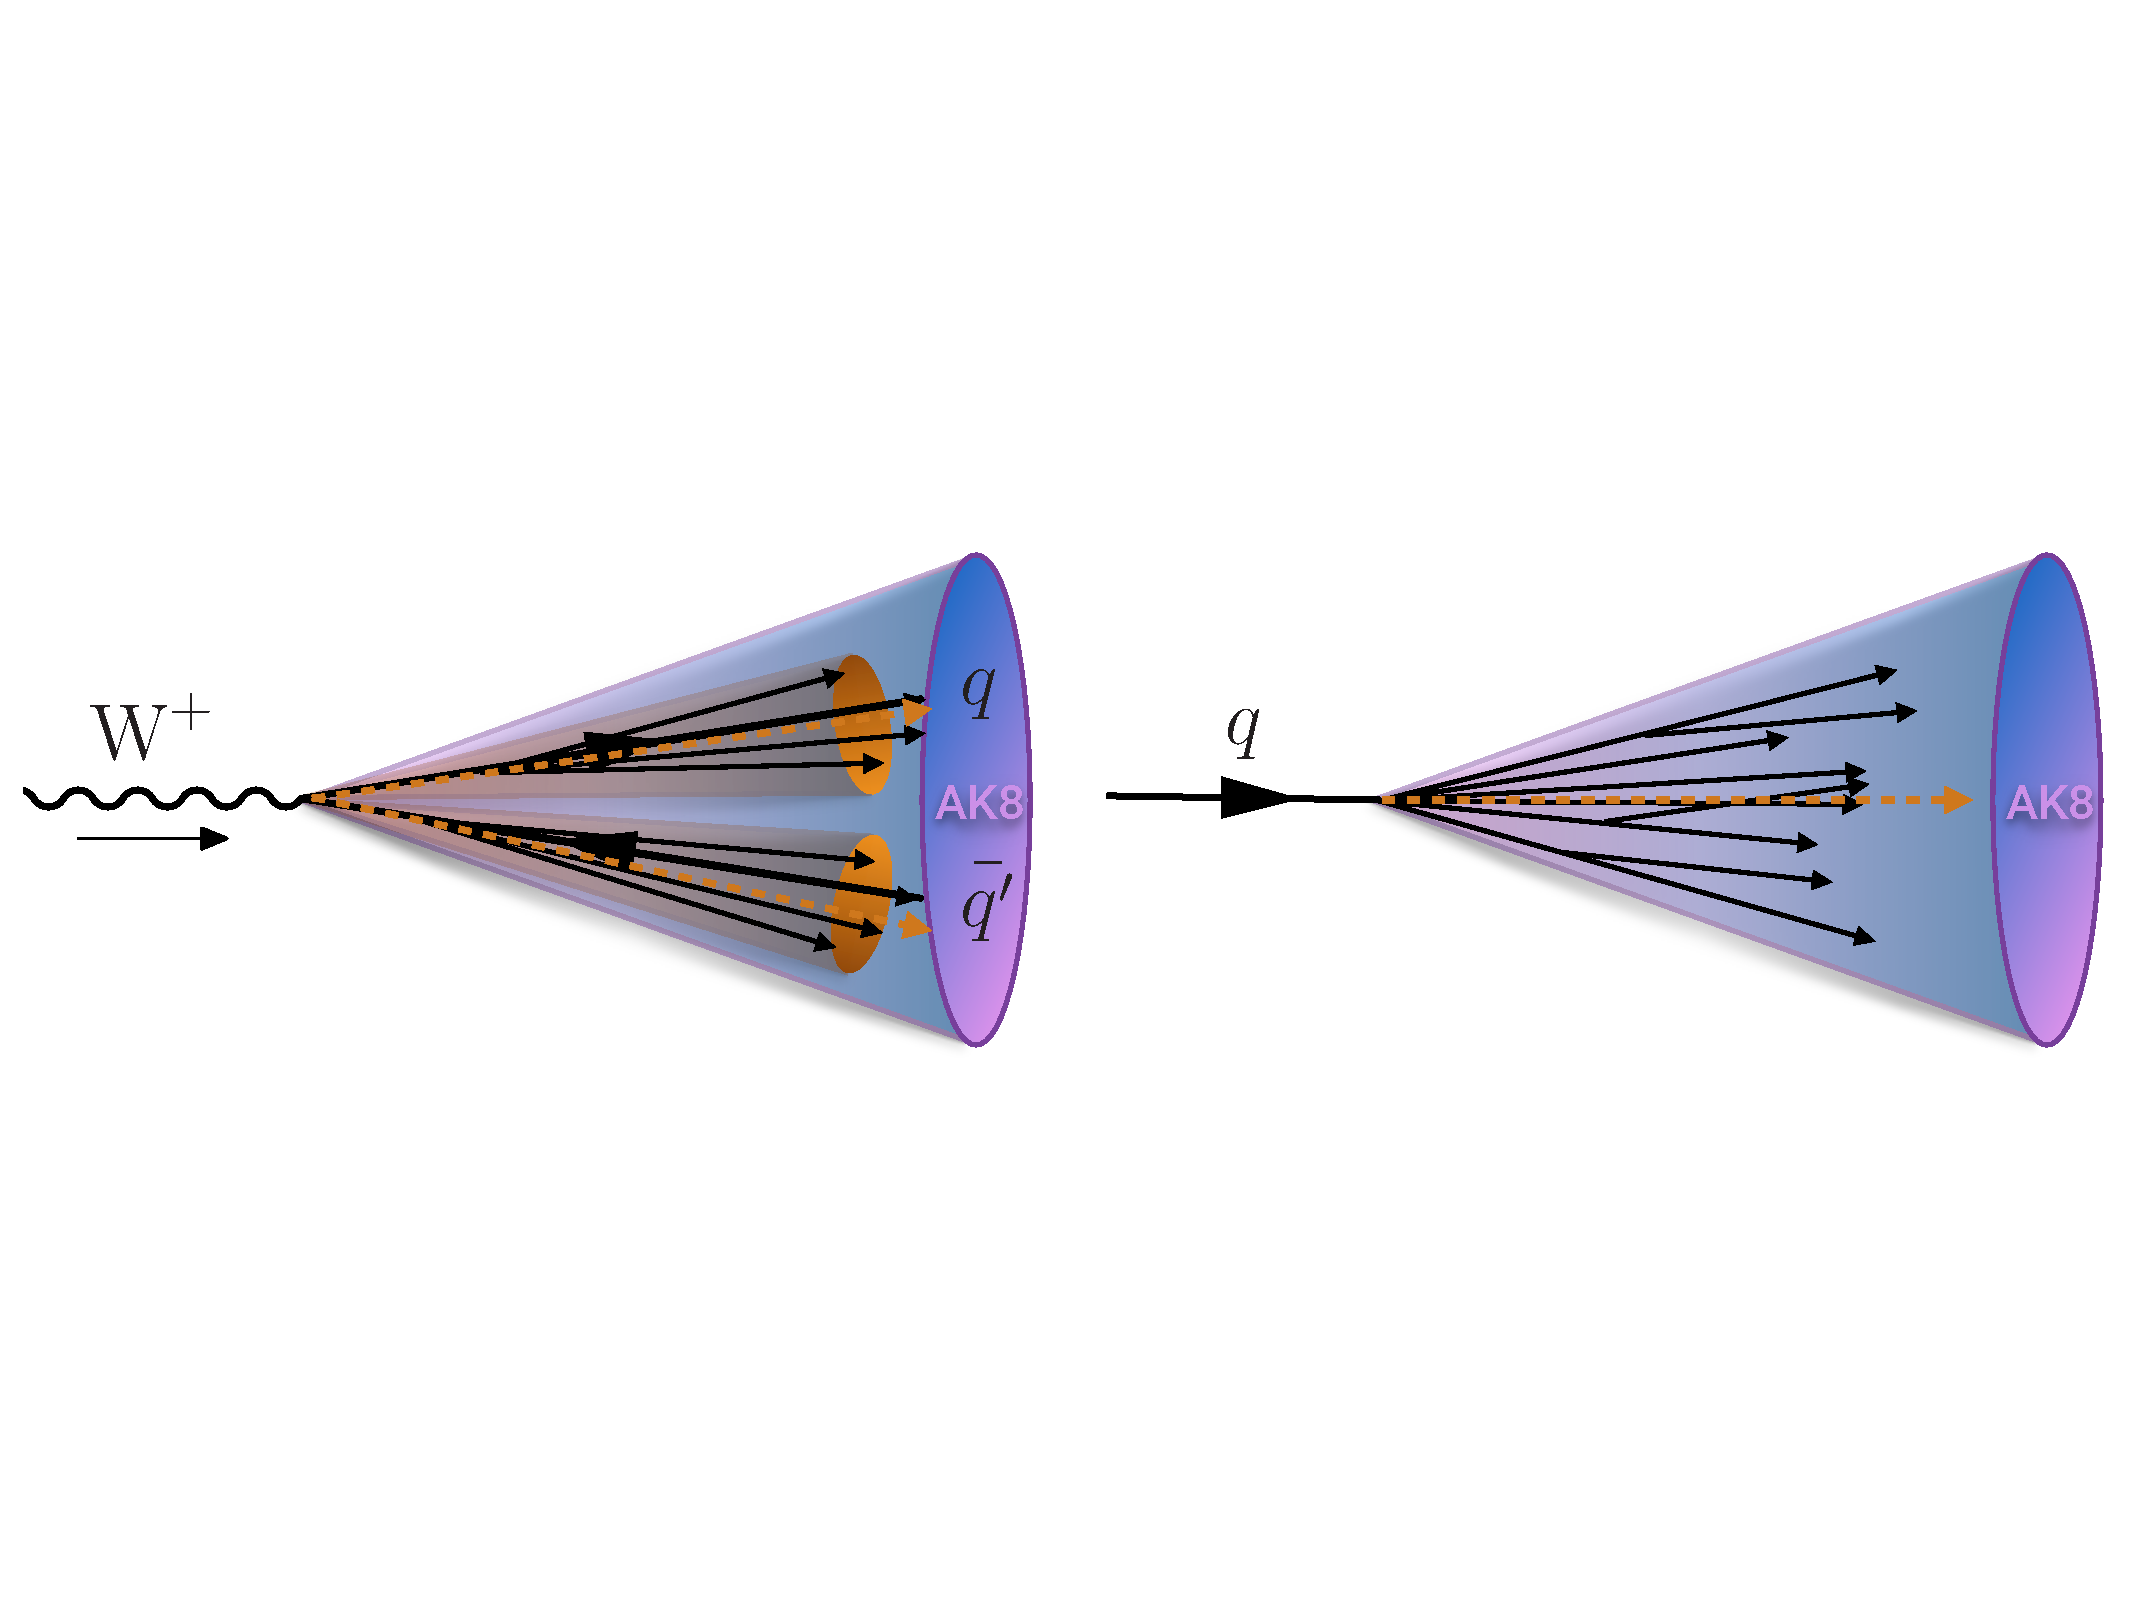
\includegraphics[width=0.790\textwidth]{figures/event_reconstruction/tau21_sketch.pdf}
     \caption{A jet stemming from the decay of a \PW will usually have two well-separated high-\pt subjets, while a jet with a single-prong origin consists of several large angel splittings.}
     \label{fig:objreco:onevstwoprong}
 \end{figure}
 
 The N-subjettiness algorithm~\cite{Thaler:2010tr} takes advantage of this fact by attempting to count the number of hard subelements within a jet. This is quantified through the n-subjettiness variable, $\tau_N$, defined as
 

 \begin{equation}
 \tau_N = \frac{1}{d_0} \sum_k p_{T,k}\textrm{min}( \Delta R_{1,k},\Delta R_{2,k}...,\Delta R_{N,k})
 \end{equation} 

where k runs over all the jet constituents, $p_{T,k}$ is the constituent transverse momentum and $\Delta R_{i,k}$ is the distance between the constituent and candidate subjet axes. These subjet axes are obtained through a one-pass optimization procedure which minimizes N-subjettiness~\cite{Thaler2012}. The normalization factor in front is given as

 \begin{equation}
d_0 = \sum_k p_{T,k} R_0
 \end{equation} 

where $R_0$ corresponds to the cone size of the initial jet. With this definition, jets with $\tau_N=0$ have most of its constituents aligned along the subjet axes. However, if $\tau_N>>0$, a large fraction of the energy is radiated away from the subjet directions and are more likely to have more than N subjets.
In CMS, and as recommended by the authors in~\cite{Thaler:2010tr}, the ratio $\tau_2/\tau_1$ is used to discriminate W jets from QCD jets. The reason for this is that, while 
signal jets are expected to have a large $\tau_1$, quark/gluon can similarly have large $\tau_1$ due to the diffuse radiation present. However, QCD jets with a large $\tau_1$ tend to have an equally large $\tau_2$, while signal jets do not, hence the ratio of the two provides greater separation power. In CMS, the n-subjettiness algorithm is by default applied to ungroomed jets.
The distribution of $\tau_{21}$ for signal and background jets with different pileup subtraction algorithms applied are shown in Figure~\ref{fig:objreco:tau21}, where $\tau_21$ in combination with PF+PUPPI (green) yields a distribution most similar to the generated one (black).

\begin{figure}[ht] 
    \centering 
    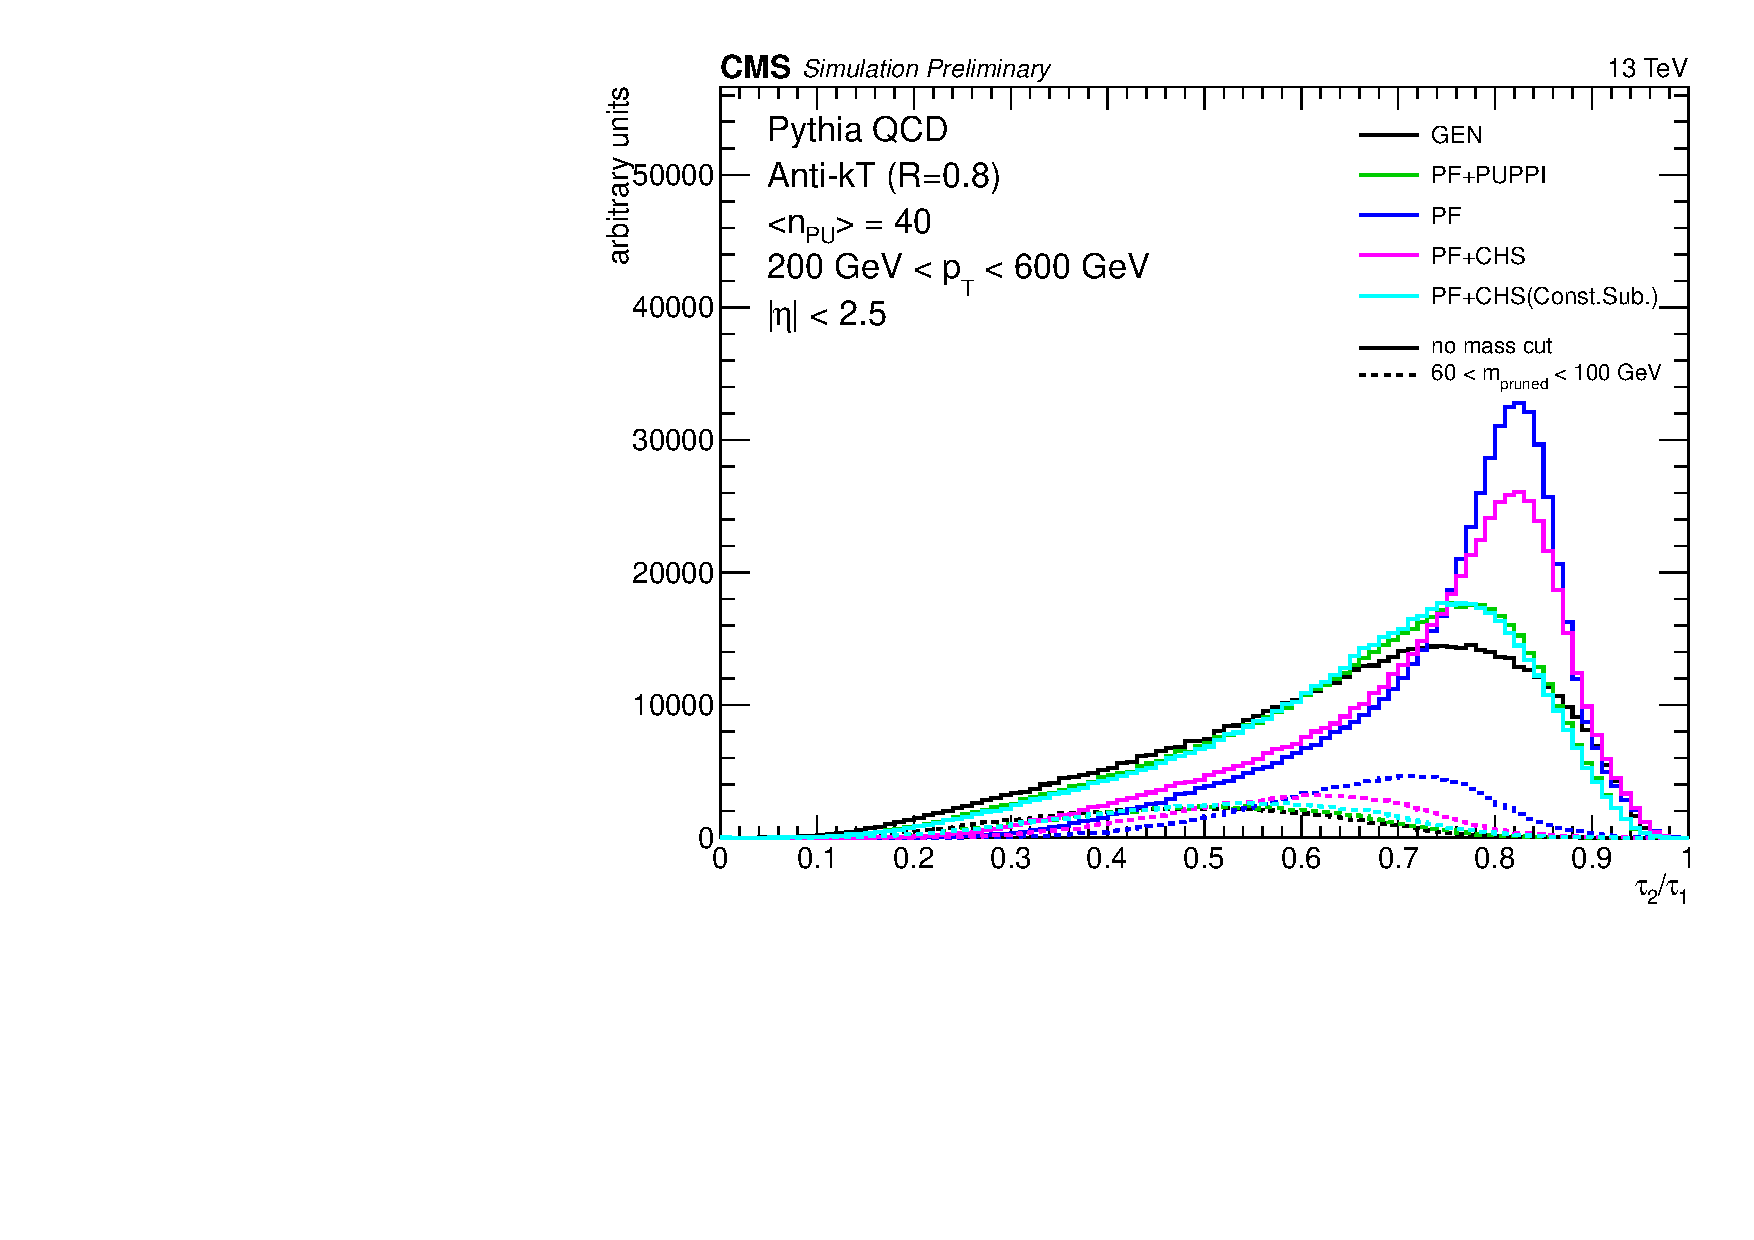
\includegraphics[width=0.490\textwidth]{figures/event_reconstruction/sig_tau21.pdf}
    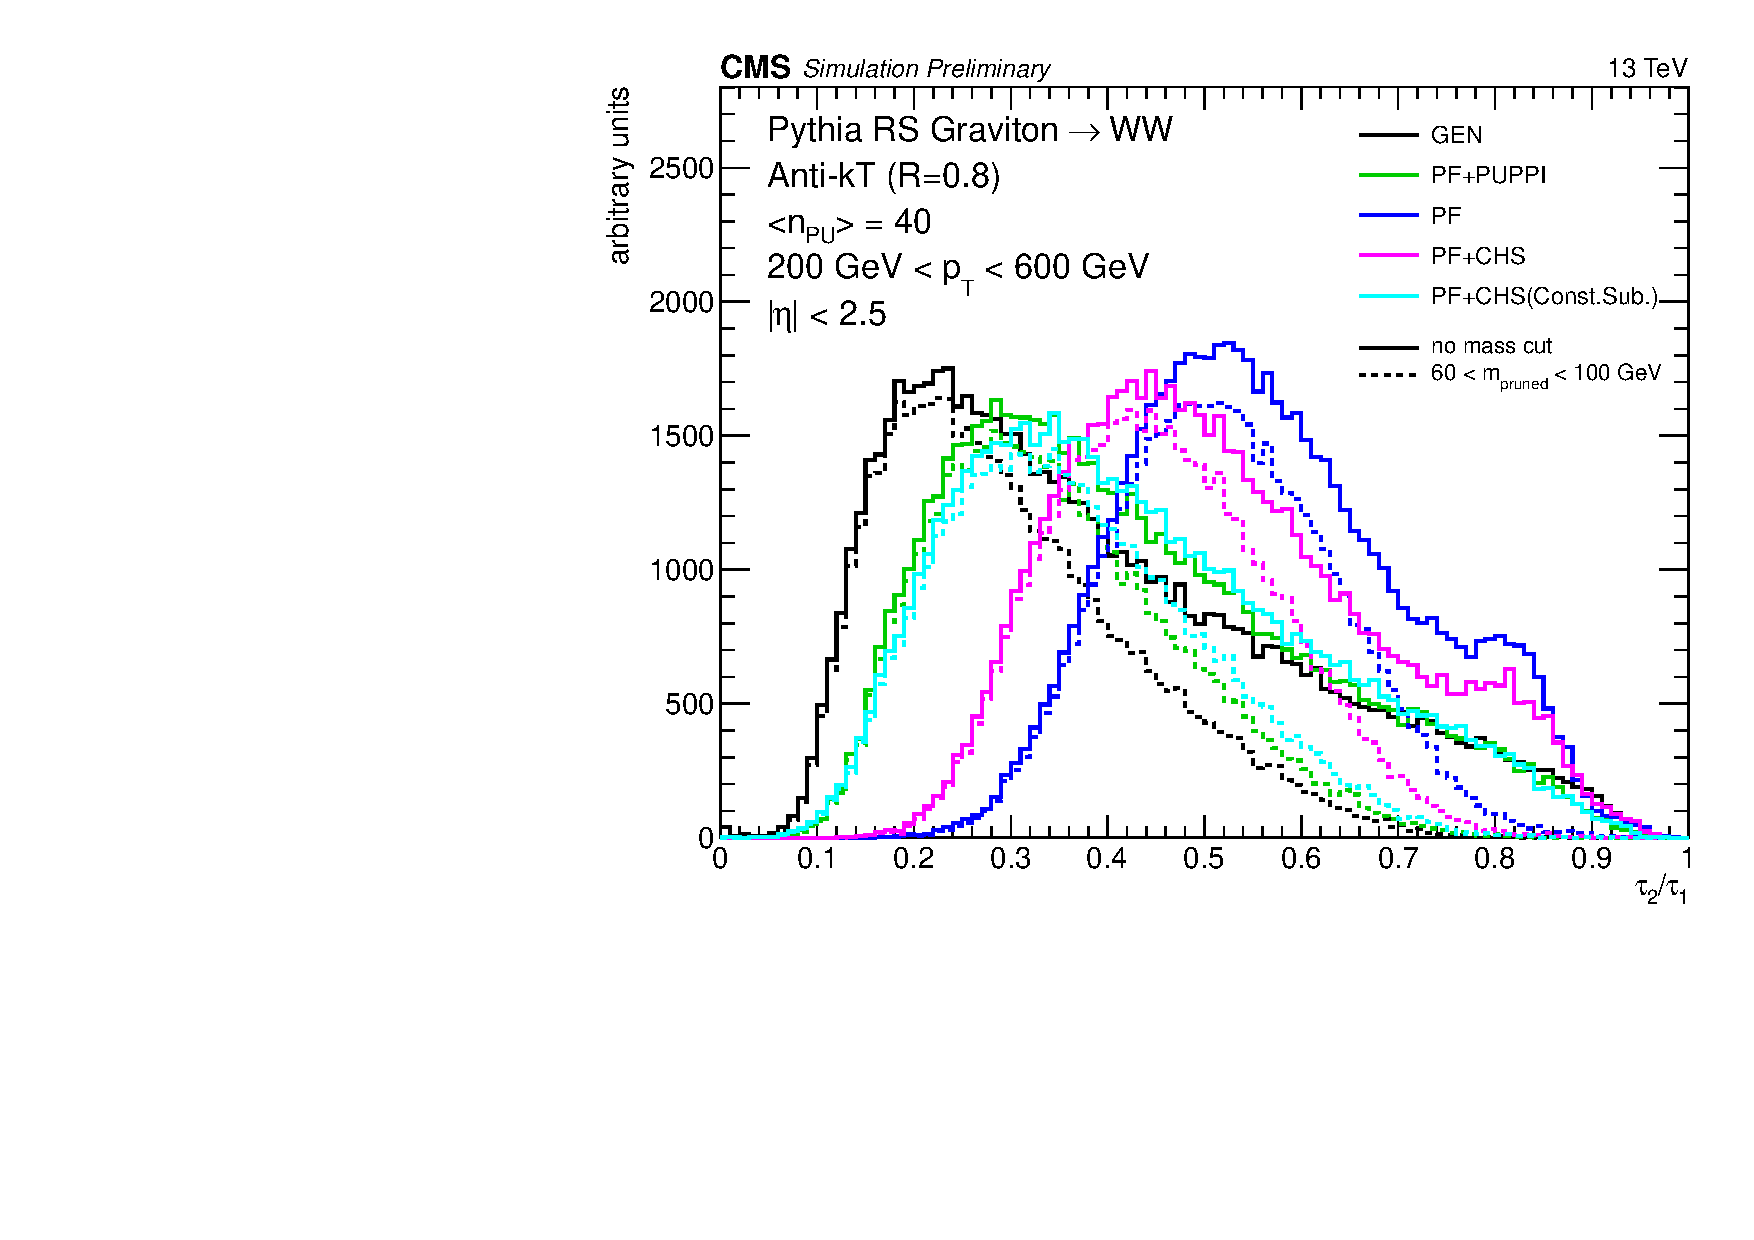
\includegraphics[width=0.490\textwidth]{figures/event_reconstruction/bkg_tau21.pdf}
     \caption{The distribution of the n-subjettiness ratio $\tau_{21}$ for signal jets (left) and background jets (right) with different combinations of pileup subtraction algorithms applied. The solid lines corresponds to the $\tau_{21}$ distribution with no mass cut applied, while the dotted lines are within a mass window of 60-100 \GeV~\cite{CMS-PAS-JME-14-001}.}
     \label{fig:objreco:tau21}
 \end{figure}


\section{Monte Carlo Simulation}

Simulated events are produced in three steps: First, a matrix element generator simulates the hard scattering process and subsequent decays. Secondly, the showering and subsequent hadronization of unstable particles is performed and then finally the final state particles are passed through a full detector simulation in order to reproduce a range of experimental effects 

\textcolor{red}{\textbf{TODO!!!}}
\subsection{Matrix Element Generators}
\textcolor{red}{\textbf{TODO!!!}}
\subsection{Shower Generators}
\textcolor{red}{\textbf{TODO!!!}}


% JET SUBSTRUCTURE TECHNIQUES
\chapter{Jet substructure} 
\label{ch:substr}
\section{Jet substructure techniques}
\subsection{Jet grooming}
\subsection{Jet substructure}
\section{W-tagging algorithms}
\subsection{Performance}
\subsection{Validation}

% DIBOSON SEARCHES
\chapter{Diboson resonance searches in CMS}
\label{ch:diboson}
%\begin{singlespace}
%\setstretch{1.25}
\begin{centering}
\chapter{Search I: First search for diboson resonances at 13 TeV}
\label{searchI}
\textit{
\noindent When the LHC started its Run II data taking period in summer 2015, it would be the first time ever for a particle collider to produce collisions with center-of-mass energies as high as 13 \TeV. The Higgs boson, for which the LHC was designed to observe, had been discovered at the end of the previous data taking era, leaving us with a Standard Model that we know is either in need of extensions or only an effective theory valid in a certain energy domain. The Run II search program would therefore be oriented around two main efforts: Precision measurements of the newly discovered Higgs boson and searches for physics beyond the standard model.
\newline
\newline
I started my PhD four months before the first 13 TeV collisions took place and had to consider the following:
What was the most interesting search that could be done on a short time scale (to be presented 6 months after first collisions, which would be at the CERN end-of-year "Jamboree"), whose physics objects could be reconstructed and understood on a relatively short time scale, and would be robust enough in case there were issues with the never-before-validated 13 \TeV Monte Carlo?
\newline
\newline
The attention of the high-energy physics community has in the past years been focused on certain "hot topics": In 2018 and currently in 2019, the excitement is over leptoquarks, which could explain anomalies observed by LHCb and b-factories; in 2016 and 2017 it was diphoton resonances, with $>3 \sigma$ excesses observed at the same mass in both CMS and ATLAS. And in 2015 during the 13 \TeV LHC start-up, attention was centered on diboson resonances in the all-hadronic final state. The choice was therefore clear: My first analysis would be a search for diboson resonances in the boosted dijet final state. With a background model based on a smooth fit to data in the signal region, eliminating the need for accurate QCD MC predictions, this was a simple one-background only (QCD) analysis, feasible to finalize in one year, given dedication and sufficient effort. Despite its straightforwardness, due to observed 8 TeV excesses, it was in addition considered a high-profile analysis.
\newline
\newline
This search became one of the first "boosted" searches published with data collected with a 13 TeV center-of-mass energy, as well as the first search to take advantage of dedicated "grooming" triggers. It was published with 2.7 \fbinv of 2015 data.
}
\end{centering}
\begin{figure}[h!] 
    \centering
     \vspace*{10mm}
    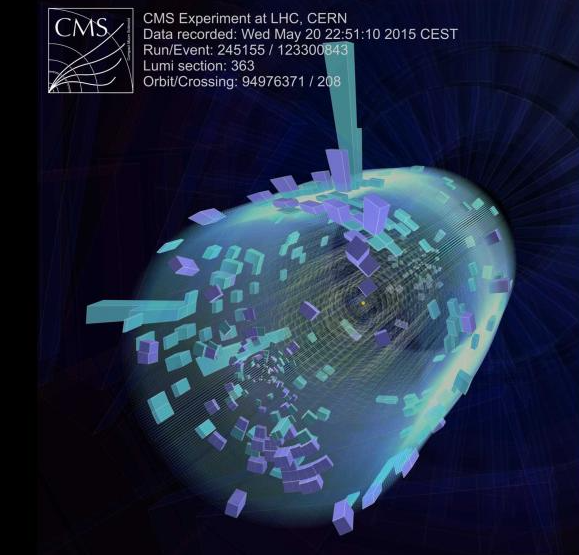
\includegraphics[height=6.5cm]{figures/analysis/search1/misc/first_coll.png}
    \vspace*{10mm}
    \caption*{\footnotesize{\textit{Published in the Journal of High Energy Physics (2017), DOI: 10.1007/JHEP03(2017)162}}}
\end{figure}
%\end{singlespace}
\clearpage
\section{A small bump}
On June 2nd, 2015, the day before CMS recorded its first ever 13 TeV event, a pre-print appeared on the arXiv titled, "Search for high-mass diboson resonances with boson-tagged jets in proton-proton collisions at $\sqrt{s} = 8$ \TeV with the ATLAS detector"~\cite{Aad2015}.
It was an analysis of the full ATLAS Run 1 dataset, corresponding to 20.3 \fbinv, searching for heavy resonances decaying to vector bosons in the all-hadronic state. The analysis documented a 3.4 $\sigma$ excess for a heavy resonance decaying to WZ with a mass of around 2 \TeV.
The corresponding CMS analysis, published the previous year, had a 1.3 $\sigma$ excess at roughly the same resonance mass, but was mostly compatible compatible with a WW final state hypothesis~\cite{Khachatryan:1700394}. Figure~\ref{fig:searchI:8tev} shows the corresponding dijet invariant mass spectrum as seen by ATLAS (left) and the upper limit on the production times the cross section for a $G_{Bulk}$ decaying to WW (right) as documented by CMS.

\begin{figure}[h!] 
    \centering
    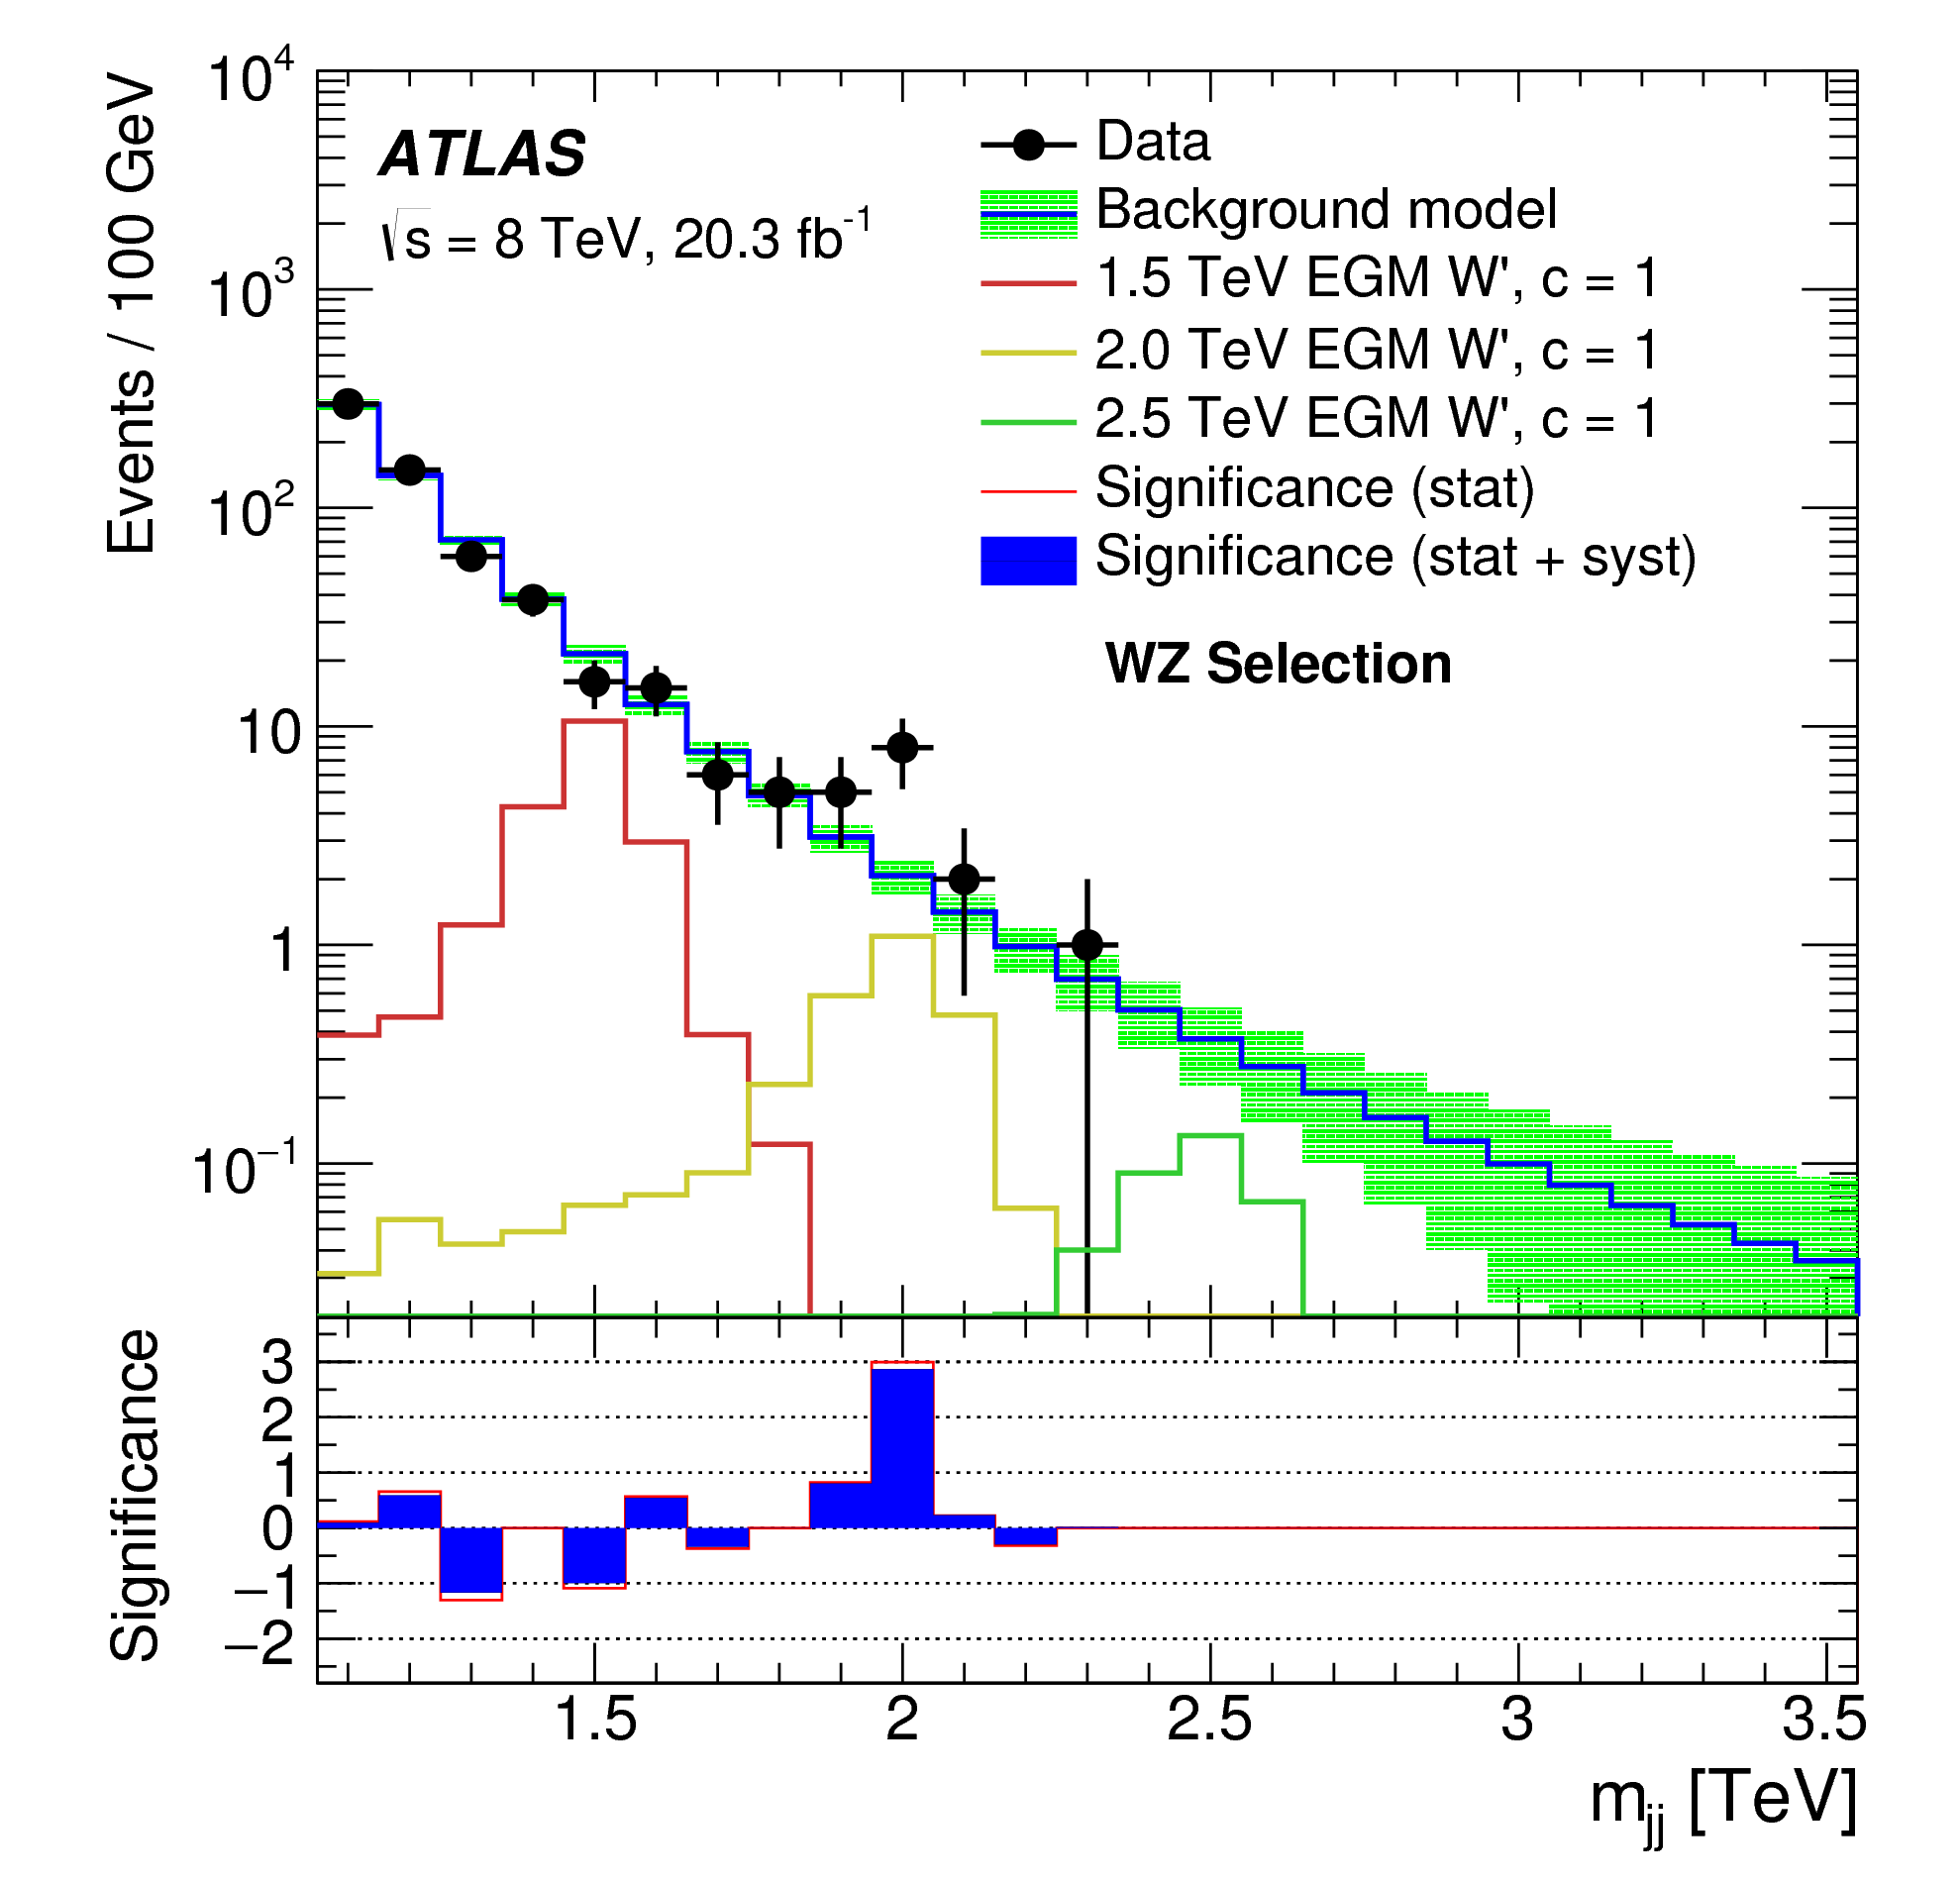
\includegraphics[width=0.4\textwidth]{figures/analysis/search1/misc/atlas_8tev.png}
    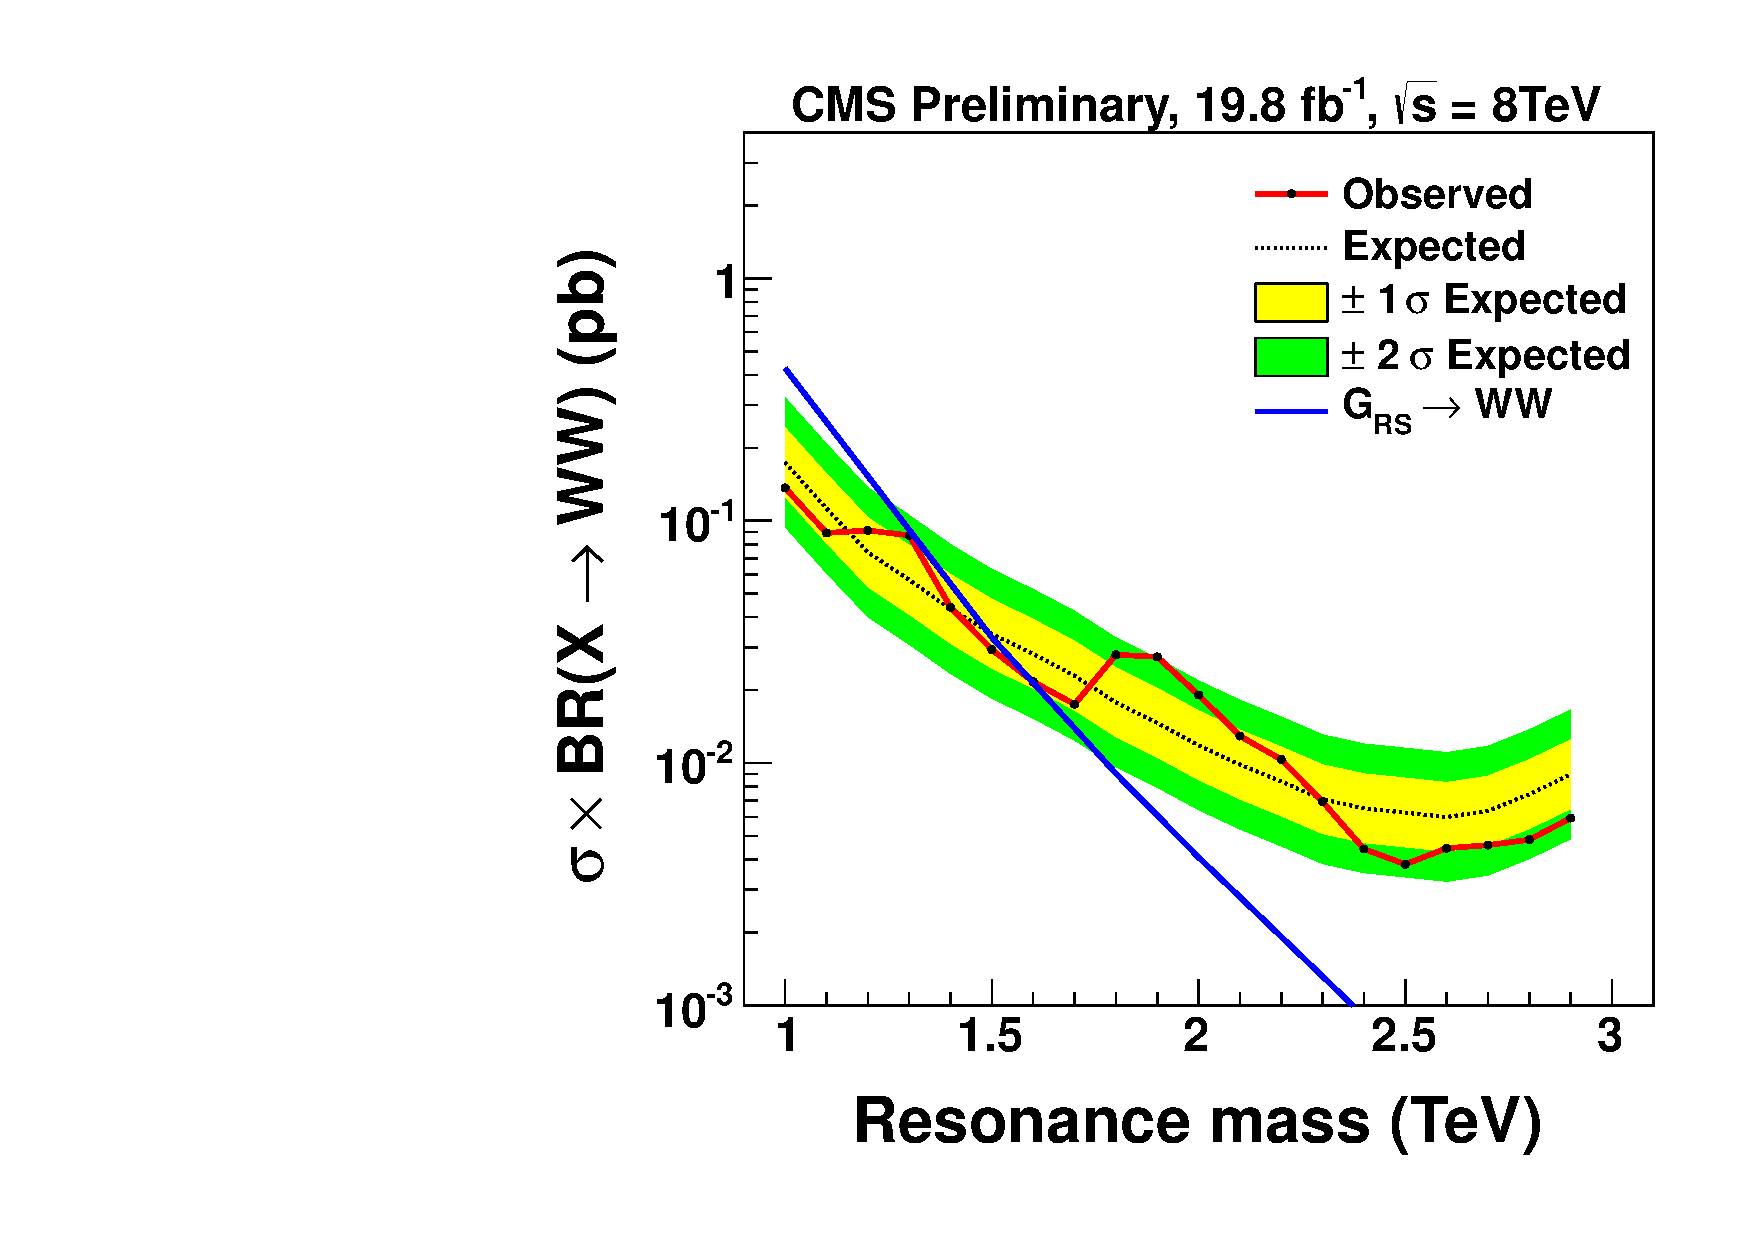
\includegraphics[width=0.4\textwidth]{figures/analysis/search1/misc/EXO-12-024_gWW.pdf}
    \caption{A "bump" corresponding to 3.4 $\sigma$ in the dijet invariant mass spectrum around 2 \TeV (left) observed by ATLAS when analyzing the full 8 \TeV dataset~\cite{Aad2015}, together with a similar excess (1.3 $\sigma$) observed in the corresponding CMS analysis~\cite{Khachatryan:1700394}.}
    \label{fig:searchI:8tev}
\end{figure}
The two measurements were found to be compatible, favoring a heavy resonance with a production cross section of around 5 femtobarn and a mass between 1.9 and 2.0 TeV decaying to either WW, WZ or ZZ~\cite{Dias:2015mhm}. Figure~\ref{fig:searchI:8tevcombo} shows the obtained p-value from the ATLAS (red) and CMS (blue) searches, as well as their combination (black). In addition to the observed excesses in the vector boson final states, another  $3 \sigma$ excess for a resonance with a mass of 1.8 \TeV had been observed in the search for heavy resonances decaying to a W and a Higgs boson~\cite{Khachatryan:2016yji} at 1.8 \TeV.
\begin{figure}[h!] 
    \centering
    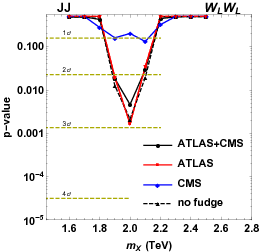
\includegraphics[width=0.25\textwidth]{figures/analysis/search1/misc/CMS_ATLAS_BulkWW_JJ_dijetfit_p.png}
    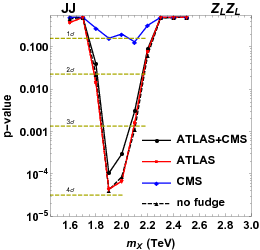
\includegraphics[width=0.25\textwidth]{figures/analysis/search1/misc/CMS_ATLAS_BulkZZ_JJ_dijetfit_p.png}
    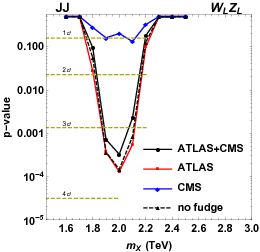
\includegraphics[width=0.25\textwidth]{figures/analysis/search1/misc/CMS_ATLAS_WZ_JJ_dijetfit_p.png}
    \caption{p-values as a function of resonance mass obtained with an emulation of the ATLAS (red) and CMS (blue) searches as well as the combination of the two (black). Here for a \PW\PW (left), \PW\PZ (middle) and \PZ\PZ (right) hypothesis~\cite{Dias:2015mhm}.}
    \label{fig:searchI:8tevcombo}
\end{figure}
The combination of the excesses and the timing of the ATLAS paper, naturally led to some excitement, and in the coming weeks, the arXiv was flooded with theory papers attempting an explanation of the deviations.\newline
In addition, one of the main benefits of increasing the LHC center-of-mass energy from 8 to 13 \TeV was that the partonic luminosity would increase.
One could therefore expect the same number of signal events in the 20 \fbinv data set collected with a center-of-mass energy of 8 TeV, for a considerably smaller luminosity with a center-of-mass energy of 13 TeV. Figure~\ref{fig:searchI:8vs13reach} shows the system mass that can be probed with the expected 2015 integrated luminosity of 3 \fbinv collected with a center-of-mass energy of 13 TeV, as a function of the probeable mass with 20 \fbinv of 8 TeV data for different partonic channels of qq, qg, and gg. For example, a 2 \TeV mass resonance would be observable in both datasets.
% The probable 13 \TeV mass is defined by finding the system mass which results in the same number of expected events at 8 \TeV, if assuming cross sections scale with partonic luminosity and $1/m^2$. Three different partonic scattering channels are considered: qq, qg and gg. We see that, for instance for a resonance with a mass of 2000 \GeV, the reach at 13 \TeV is 2241(gg), 2091(gq), 1851(qq, one type) and 2046(qq, all types) \GeV.
\begin{figure}[h!] 
    \centering
    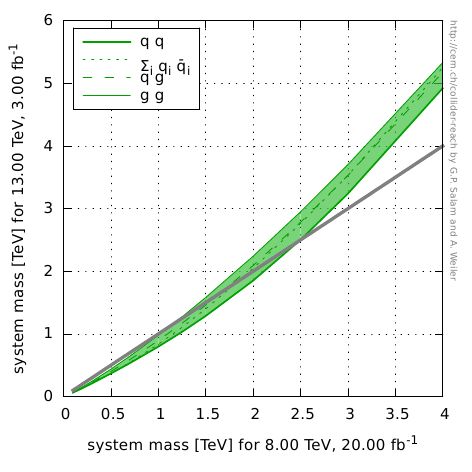
\includegraphics[width=0.50\textwidth]{figures/analysis/search1/misc/colliderReach.png}
    \caption{The system mass that can probed with 3 \fbinv of 13 \TeV data (y-axis) as a function of the probe-able system mass with 20 \fbinv of 8 \TeV data (x-axis) for different partonic channels (generated with~\cite{collreach}).}
    \label{fig:searchI:8vs13reach}
\end{figure}
We therefore expected that the small excess observed in the VV all-hadronic final state would be observable in the 2015 dataset if the signal was genuine.

\section{Analysis strategy}

When a resonance X with a mass above 1 TeV decays into a vector-boson pair, the bosons have a very high energy ($\tilde\PT=\mX/2=500 \GeV$, assuming X is produced at rest) is referred to as boosted. The decay products of a hadronically decaying boosted vector boson will therefore not appear as back-to-back in the lab frame but rather be collimated, as described in Section~\ref{sec:objreco:substructure}. This results in a final state with two high-pt, large-radius jets, such that the AK algorithm with an R=0.8 is expected to fully contain the two quarks coming from the vector boson decay. This is illustrated in Figure~\ref{fig:searchI:merged}.
\begin{figure}[h!] 
    \centering
    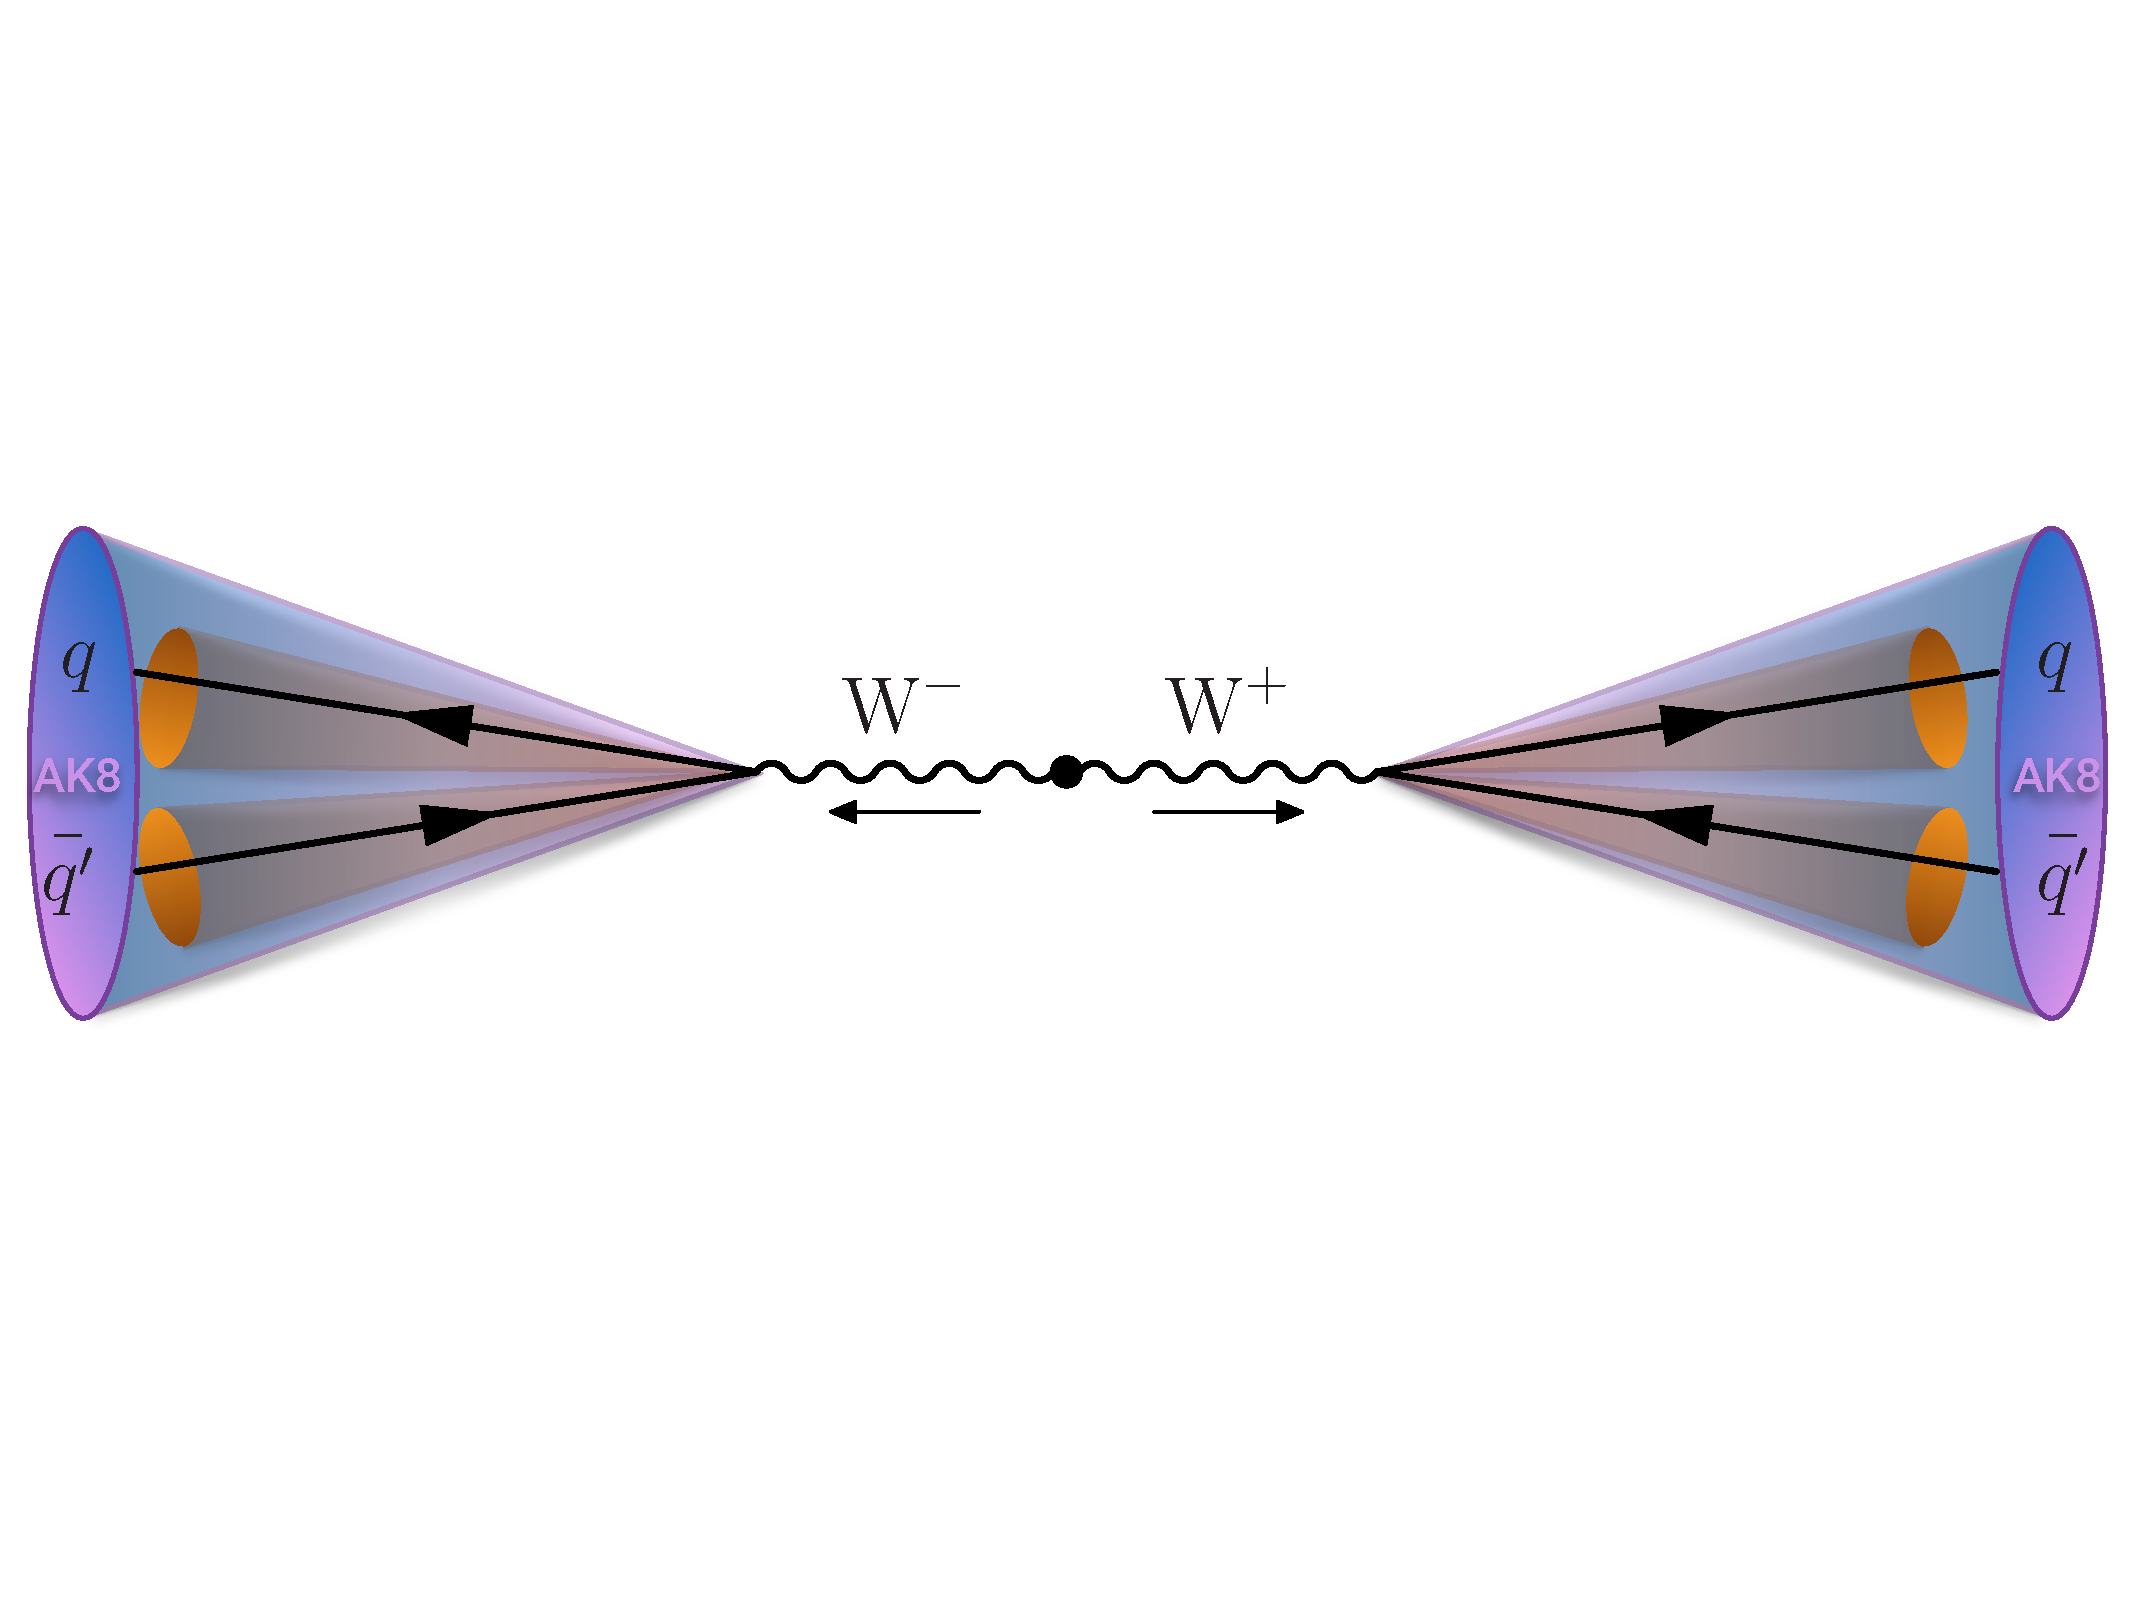
\includegraphics[width=0.70\textwidth]{figures/event_reconstruction/WWqqqq_merged_small.pdf}
    \caption{If a heavy ($>1 \TeV$) resonance decays into vector bosons, the transverse momentum of each boson will be large and its decay products are merged into one single large cone AK8 jet.}
    \label{fig:searchI:merged}
\end{figure}
The two jets are each expected to have a mass around the W or Z boson mass, and some intrinsic substructure stemming from their two-pronged decay. The invariant mass of the dijet system, \mjj, should be roughly equal to the resonance mass \mX. This dijet system is the final state under scrutiny and the dijet invariant mass is the parameter of interest. The final states of WW, ZZ, and WZ would produce similar final states. \par
The main background for such an analysis is QCD multijet events. As mentioned in Section~\ref{sec:objreco:substructure}, quark/gluon jets can obtain a high mass due to diffuse radiation and QCD processes have such a large cross section that the number of QCD jets with a mass compatible with the W mass can be large. In order to discriminate between the two, we take advantage of three properties. First, the groomed mass of signal and background jets should be very different. Second, signal jets should appear two-prong like, as opposed to quark/gluon jets, and third, the dijet invariant mass for the signal process should peak around the resonance mass while the QCD spectrum is predicted to be smoothly falling. Section~\ref{sec:searchI:bkg} explains this assumption in more detail. The strategy therefore consists of performing a smoothness test on \mjj of the observed data, a so-called "bump-hunt", by assuming that the signal will appear as a bump on top of a smooth distribution. This is illustrated in Figure~\ref{fig:searchI:bumphunt}.
\begin{figure}[h!] 
    \centering
    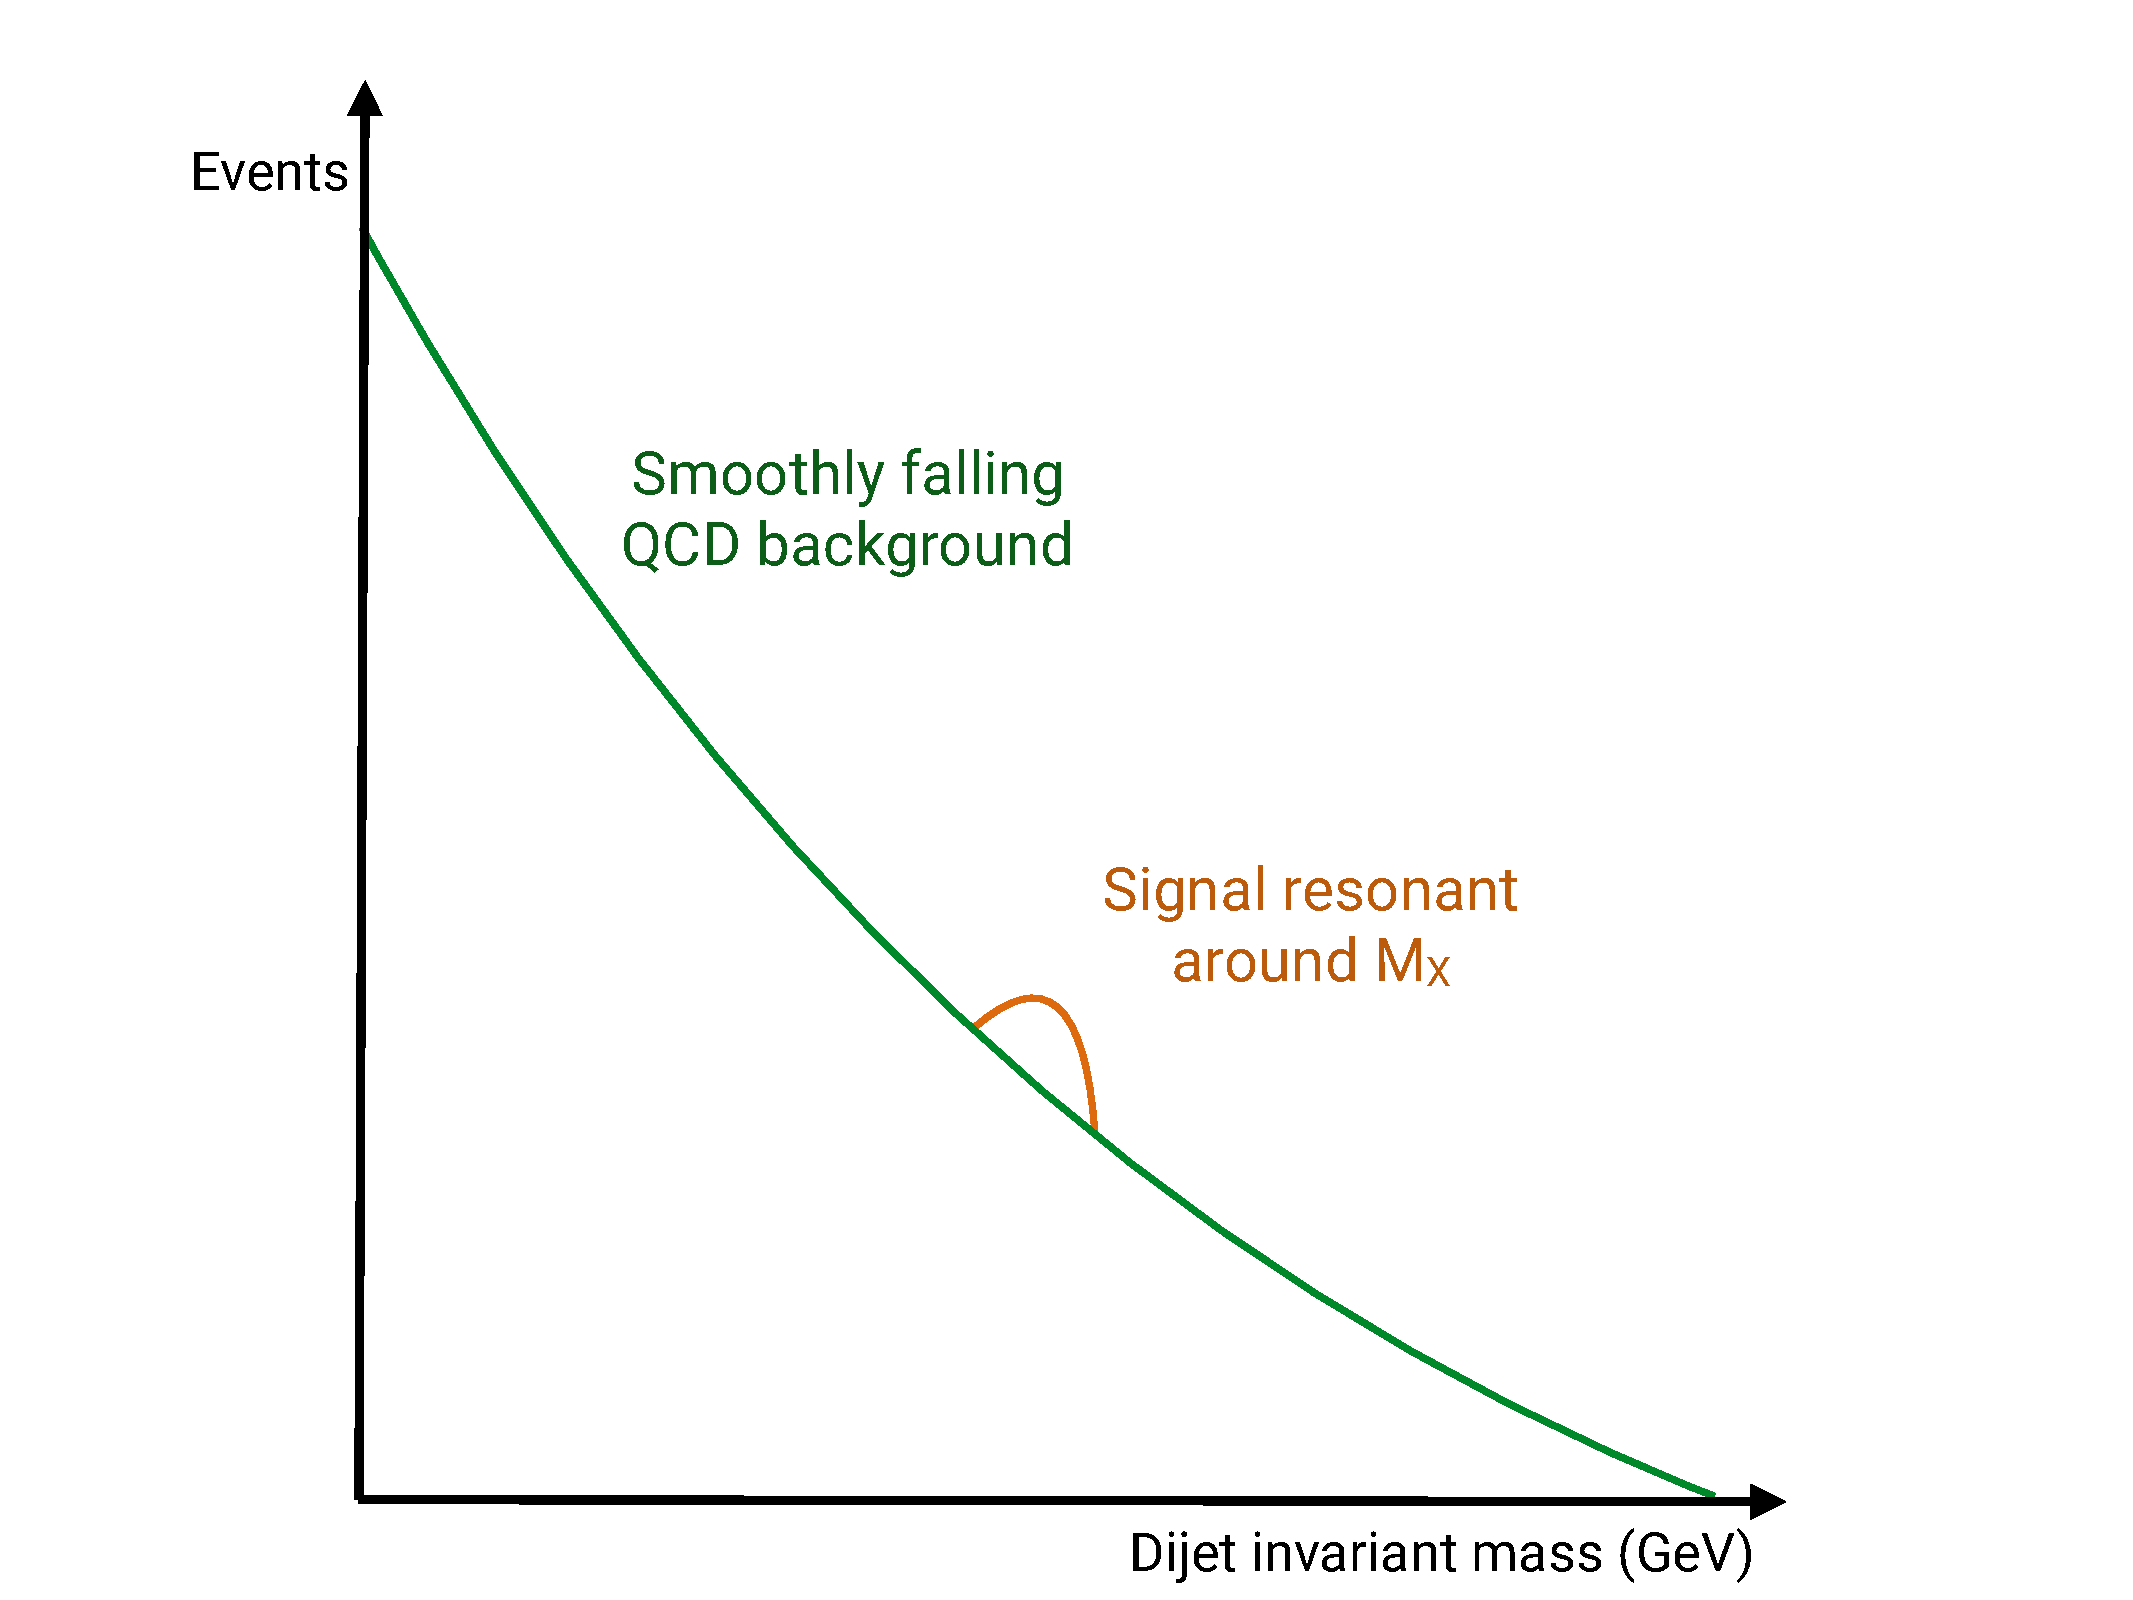
\includegraphics[width=0.49\textwidth]{figures/analysis/search1/misc/sigExtraction.pdf}
    \caption{The search strategy consists of looking for signal "bumps" in the dijet invariant mass on top of a smoothly falling QCD multijet background.}
    \label{fig:searchI:bumphunt}
\end{figure}
The benefit of such a method is that there is no need for a simulation of the background and the strategy is simple and robust. The disadvantage is that the analysis is intrinsically limited to regions where the dijet invariant mass spectrum is smooth and hence regions with discontinuities due to trigger turn-ons or kinematic selections must be avoided.

\section{Data and simulated samples}
\label{sec:searchI:samples}
The data analyzed in this search correspond to a total integrated luminosity of 2.7\fbinv collected at a center-of mass energy of 13 \TeV between June and December 2015. The instantaneous luminosity of the LHC during this run was around half of the design luminosity ($0.5 \times 10^{34} \percms$), with an average number of primary vertices per event of $<\mu>=13$. \par
The bulk graviton model (see Section~\ref{sec:theory:wed}) and the HVT model (\PWpr{} and \PZpr{}, see Section~\ref{sec:theory:hvt}) are used as benchmark signal processes. In these models, the vector gauge bosons are produced with a longitudinal polarization in more than 99\% of the cases, which leads to a 24\% higher acceptance per boson for reasons explained in Section~\ref{sec:objreco:pol}. For the HVT model, a scenario (model B) with $g_{\rm V}=3$, $c_{\rm H}=-0.976243$, and $c_{\rm F}=1.02433$ is chosen, where the heavy resonance predominantly couple to bosons and the coupling to fermions is suppressed. The bulk graviton samples were generated with $\ktilde = 0.5$. The resonance masses considered lie in the range 1.2 to 4 \TeV and are generated under the assumption of a natural width negligible with respect to the experimental resolution (narrow-width approximation). All signal samples are generated at leading order with \amcatnlo{} v2.2.2~\cite{Alwall:2014hca}. \par
Simulated samples of the production of QCD multijet events are generated to leading order using \PYTHIA version 8.205~\cite{Sjostrand:2007gs} with the CUETP8M1 tune~\cite{Khachatryan:2015pea} and are used to validate the analysis procedure.


\section{Event selection}

\subsection{Triggering}
\label{sec:searchI:trigger}
The first selection to be confronted in any analysis is the trigger selection. Due to an overwhelming QCD background in all-hadronic final states, the threshold for fully-hadronic triggers is very large in order to keep the trigger rate low (preferably around 10-30 Hz). In this analysis, we therefore decided to take advantage of triggers that place requirements on the jet's groomed mass in addition to the "standard" jet triggers based on the scalar sum of jet transverse energy \HT. These "boosted" triggers were never before tested in data, and this analysis was the first published result taking advantage of grooming at the trigger level in CMS. The following \HT-based High Level Triggers (HLT), referred to as inclusive triggers in the following, are used:
\begin{itemize}
\item \texttt{HLT\_PFHT650\_WideJetMJJ900DEtaJJ1p5},
\item \texttt{HLT\_PFHT650\_WideJetMJJ950DEtaJJ1p5}, and
\item \texttt{HLT\_PFHT800}.
\end{itemize}
Here, \emph{PFHT650} refers to a total \HT of at least 650 GeV. \emph{WideJet} means jets reconstructed with the \emph{wide jet algorithm}~\cite{2011123}, an algorithm inspired by jet grooming intended to reduce sensitivity to gluon radiation. The two AK R=0.4 jets with the largest \PT in the event are used as seeds. Geometrically close jets are then combined into the closest jet seed if they are within $\Delta R = \sqrt{(\Delta \eta)^2+\Delta \phi)^2}$, and these two jets form a dijet system used for further selections. \emph{MJJ900} refers to a wide-jet dijet mass of at least 900 GeV, and \emph{DetaJJ1p5} means there is an additional cut on the $|\Delta \eta|$ between the two wide jets for reasons that will be explained below. In addition, two triggers based on jet grooming are used. These require a trimmed jet mass (see Section 3.5.1) of 30 and 50 GeV, yielding the triggers:
\begin{itemize}
\item \texttt{HLT\_AK8PFJet360\_TrimMass30} and
\item \texttt{HLT\_AK8PFHT700\_TrimR0p1PT0p03Mass50}.
\end{itemize}
The tuneable parameters for the trimming algorithm at HLT are $r_{sub}=0.2$ and $p_{T,frac}=0.03$. The \texttt{HLT\_AK8PFJet360\_TrimMass30} trigger is seeded by single-object Level 1 triggers with jet $p_T$ thresholds of 176 or 200 GeV (\texttt{L1\_SingleJet176} or \texttt{L1\_SingleJet200}), and the remaining triggers require an online \HT{}$>$150 or 175 GeV (\texttt{L1\_HTT150} or \texttt{L1\_HTT175}).\par
In order to avoid any kinks in the dijet invariant mass spectrum due to the presence of a trigger turn-on, we determine the dijet invariant mass at which the analysis triggers are fully efficient ($>99\%$), and only consider signal events above this value. In order to estimate the trigger efficiency, we use a trigger with a lower \HT threshold, \texttt{HLT\_PFHT650}, as a reference trigger. This trigger has a prescale of 40, meaning events are only recorded one out of 40 times. It is seeded by L1 \HT triggers with thresholds of 150 or 175 GeV. We then define the efficiency as
\begin{equation*}
\textrm{Efficiency} = \frac{N_{trigger+ref}}{N_{ref}}  
\end{equation*}
where $N_{trigger+ref}$ corresponds to the number of events passing the trigger under study as well as the reference trigger, and $N_{ref}$ corresponds to the number of events passing the reference trigger. Figure~\ref{fig:searchI:trigger-fits} shows the trigger turn-on curves as a function of dijet invariant mass for jets where one of the jets is required to have a pruned mass larger than 65 GeV (in other words, compatible with a W jet). A sharp turn-on for the inclusive triggers (top left) is observed, reaching the 100\% efficiency plateau for dijet masses of around 1.0--1.1 TeV. The grooming triggers, however, turn on more slowly and are not fully efficient until dijet invariant masses reach around 1.2 TeV (top right). The real power of the grooming triggers become clear when considering them in addition to the \HT-based triggers. The bottom plot in Figure~\ref{fig:searchI:trigger-fits} compares the trigger turn-on curves as a function of dijet invariant mass for jets passing one of the three inclusive triggers only, one of the grooming triggers only, and when combining all of them. Here, one can see that the 99\% efficiency threshold is lowered by 75 \GeV when including the substructure triggers, once substructure is required at analysis level. This combination of triggers allowed the analysis to consider dijet invariant masses as low as 1 TeV.
\begin{figure}[h!]
\centering
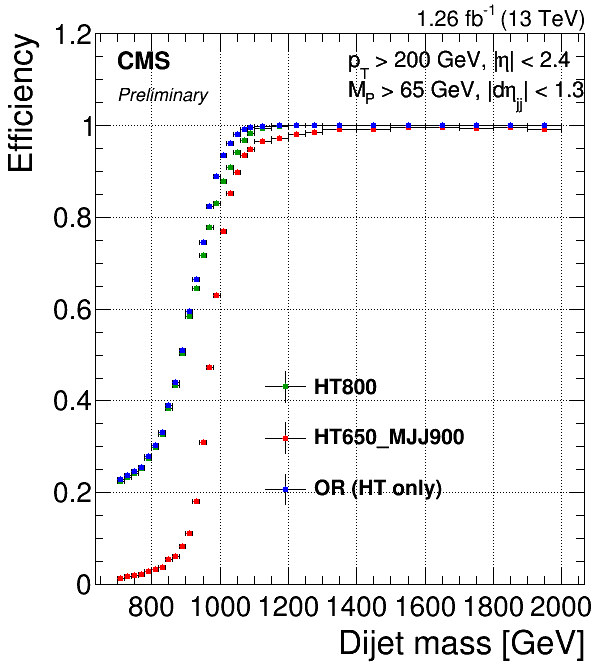
\includegraphics[width=0.4\textwidth]{figures/analysis/search1/AN-15-211//triggereffMjj-HT.png}
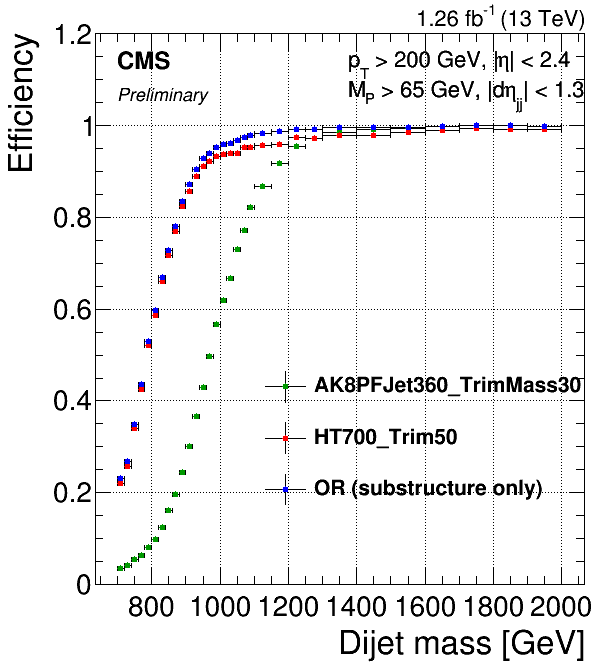
\includegraphics[width=0.4\textwidth]{figures/analysis/search1/AN-15-211//triggereffMjj-SUBST.png}\\
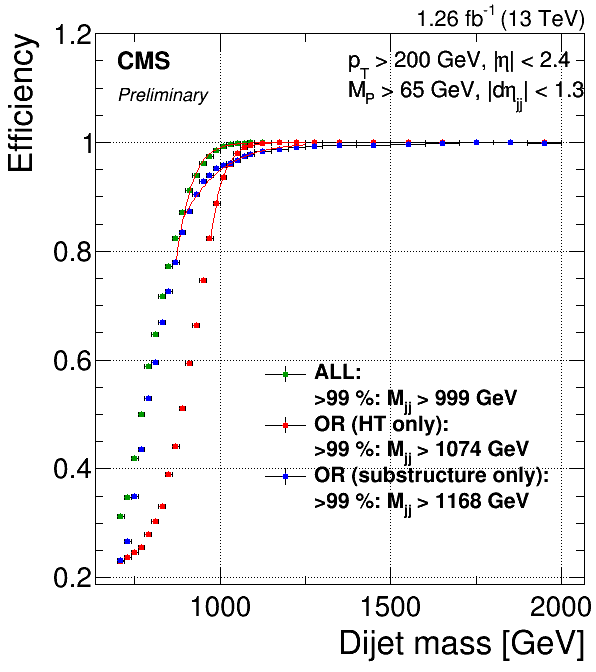
\includegraphics[width=0.4\textwidth]{figures/analysis/search1/AN-15-211/triggereffMjj-ALL.png}
\caption{Top: Efficiency for the inclusive triggers (top left) and the grooming triggers (top right) as a function of dijet invariant mass for jet pairs where one jet has a pruned mass larger than 65 GeV. Bottom: Comparison of trigger efficiencies for jets passing one of the HT-triggers only (red), for jets passing one of the grooming-triggers only (blue) and for jets passing one of the HT-triggers or one of the grooming triggers (green). Here as a function of dijet invariant mass for all jet pairs passing loose selections and where one jet has a pruned mass larger than 65 GeV. The 99\% efficiency threshold is lowered by 75 \GeV when including substructure taggers.}
\label{fig:searchI:trigger-fits}
\end{figure}
As a measure of the performance of the grooming triggers, we have in addition looked at the trigger efficiencies as a function of the offline groomed mass (using the pruned and softdrop algorithms described in Sections~\ref{sec:objreco:pruning} and ~\ref{sec:objreco:softdrop}), for the grooming trigger with the lowest mass threshold (30 \GeV). This is shown in Figure~\ref{fig:searchI:grooming-mj-trigger}, where an additional cut on the jet transverse momentum of one of the jets of 600 GeV is required and no other mass cut is applied. The trigger plateau is reached for offline groomed-jet masses around 50 GeV. 
\begin{figure}[h!]
\centering
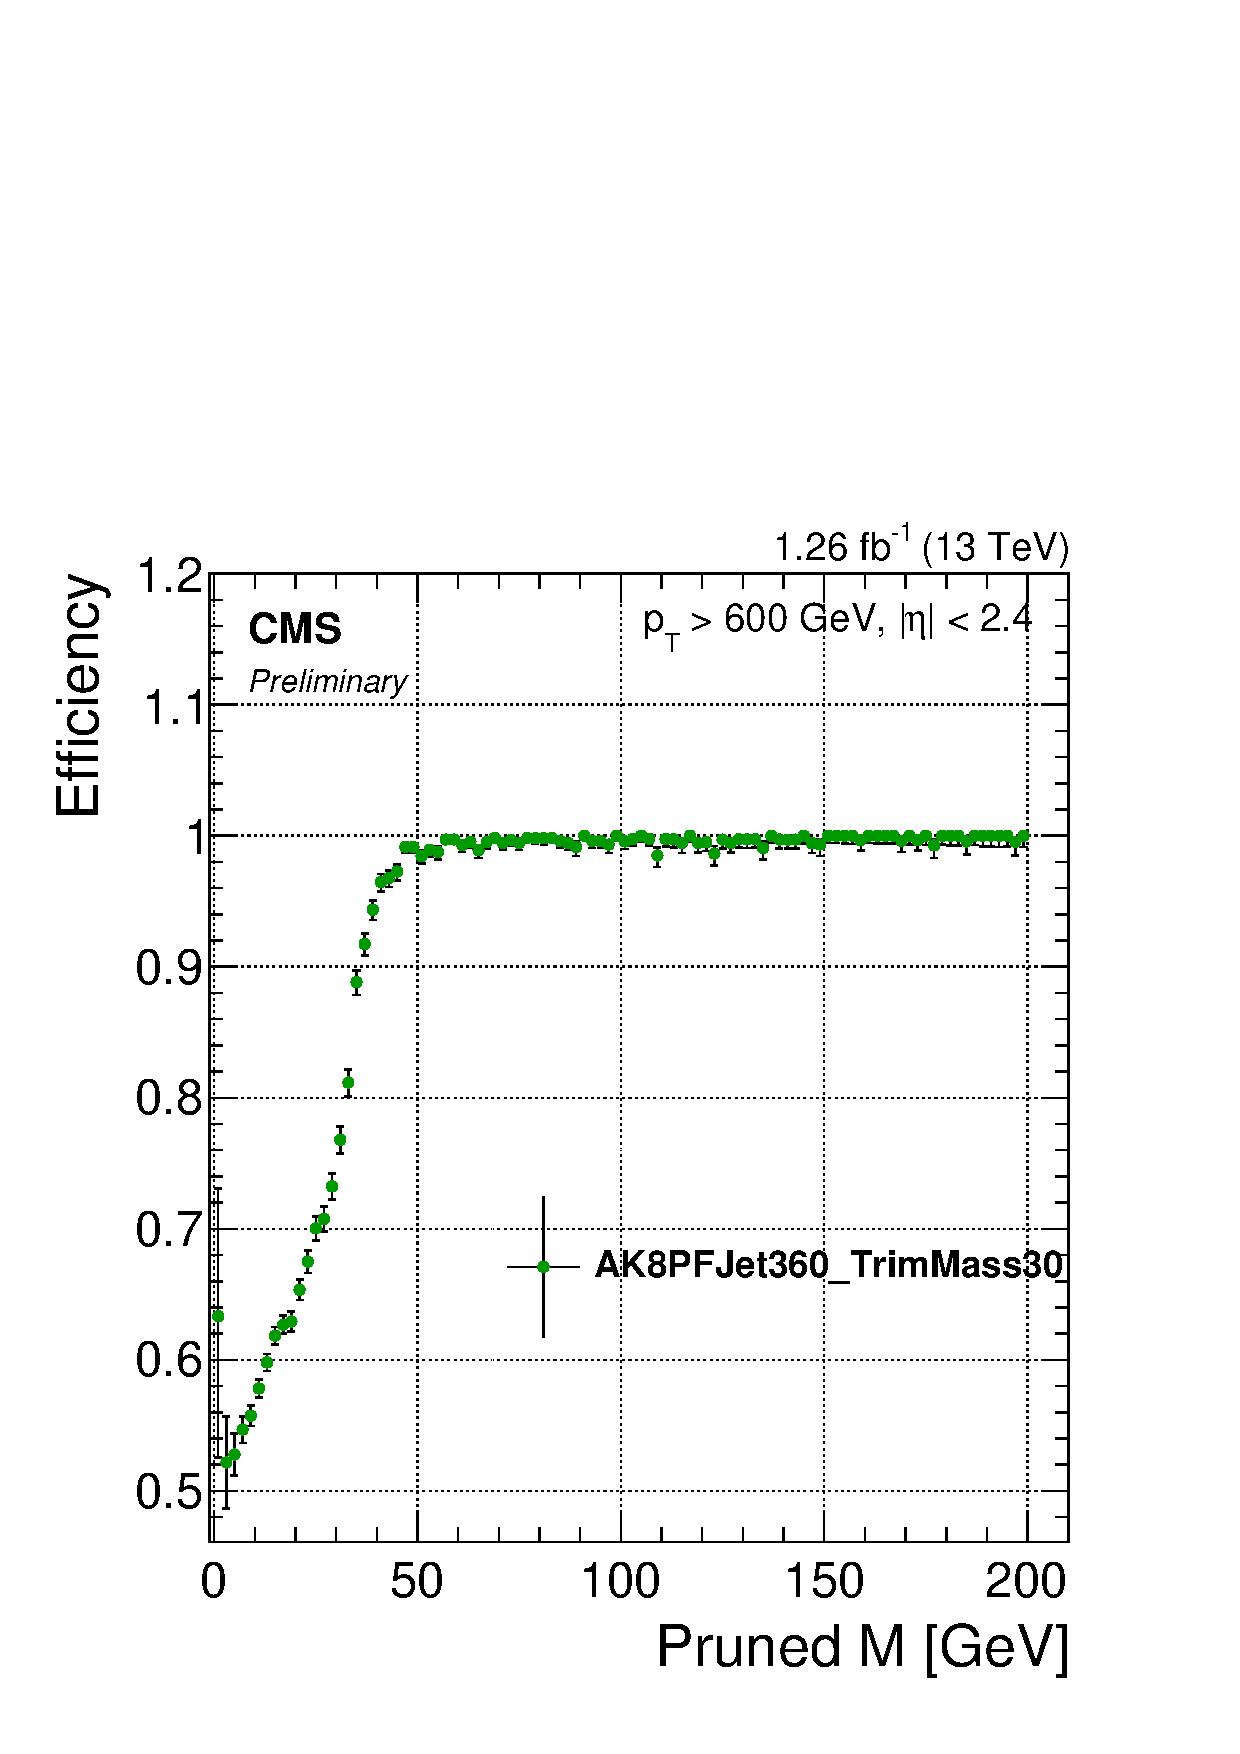
\includegraphics[width=0.4\textwidth]{figures/analysis/search1/AN-15-211//triggereff-prunedmass600.pdf}
\includegraphics[width=0.4\textwidth]{figures/analysis/search1/AN-15-211//triggereff-sdmass.pdf}
\caption{Efficiency for the lowest threshold grooming trigger as a function of pruned-jet (left) and softdrop-jet (right) mass for jets with $\PT > \unit{600}{\GeV}$.}
\label{fig:searchI:grooming-mj-trigger}
\end{figure}

\subsection{Preselection} 
\label{sec:searchI:preselection}
After trigger selections, and the corresponding requirement of a dijet invariant mass above 1 \TeV to ensure a smoothy falling background, we begin the process of maximizing the signal significance while keeping the background low. This is done by optimizing the selection requirements on the jets. The jets used in this analysis are clustered with the anti-\kt{} jet clustering algorithm with a clustering parameter of $R=0.8$ (see Section ~\ref{sec:objreco:jets}) to allow containment of the full vector-boson decay products. Since a minimum transverse momentum of 200 \GeV is required for the decay products of a W/Z to be fully contained within an R=0.8 jet, events are further selected by requiring at least two jets with $\PT > \unit{200}{\GeV}$. These are in addition required to be central, with an $|\eta| < 2.4$. The two highest \PT jets in the event passing these criteria are selected as potential vector boson candidates. As our main background is QCD multijet events, we further take advantage of the fact that the angular distribution between these, mainly t-channel, processes are very different from the s-channel signal processes under study. The crossection for QCD t-channel processes as a function of the opening angle with respect to the beam axis ($\theta*$), exhibit a pole around $\cos \theta*=1$, meaning QCD t-channel jets are mostly produced in the forward direction, with an opening angle with respect to the beam axis close to zero. The signal jets on the other hand, produced through an s-channel process, are concentrated in the barrel region. We therefore require the jets to have a separation of $|\Delta\eta|<1.3$ in order to reduce the QCD multijets background. The distribution of $|\Delta\eta|$ between the two highest-\PT jets for QCD, as well as for different signal scenarios, is shown in Figure~\ref{fig:searchI:detaopt}.
\begin{figure}[h!]
\centering
\includegraphics[width=0.4\textwidth]{figures/analysis/search1/misc/deta_opt.png}
\caption{ $|\Delta\eta|$  between the two highest-\PT jets for QCD jets and jets stemming from different signal scenarios.}
\label{fig:searchI:detaopt}
\end{figure}
A cut of $|\Delta \eta|_{jj}<1.3$ removes the t-channel pole at $\cos \theta* = 1$ and is in addition found to yield the highest signal sensitivity. In addition to these requirements on the jets themselves, a veto on jets overlapping with leptons is applied. Here the overlap $\Delta R(\text{jet},\text{lepton})$ between the jet candidate and a lepton is required to be larger than 0.8. Leptons used for this veto are required to pass the identification requirements described in Section~\ref{sec:objreco:electrons} and~\ref{sec:objreco:muons}, have a transverse momentum larger than 35 (30) GeV, and a pseudorapidity smaller than 2.5 (2.4) in the case of electrons (muons). The \PT, $\eta$, dijet invariant mass, and $|\Delta \eta|_{jj}$ distribution for the two leading jets in the event after the above preselections have been applied is shown in Figure~\ref{fig:kinematics-all}.
\begin{figure}[h!]
\centering
\includegraphics[width=0.4\textwidth]{figures/analysis/search1/AN-15-211/controlplots/silverjson/Pt_WSignal.pdf}
\includegraphics[width=0.4\textwidth]{figures/analysis/search1/AN-15-211/controlplots/silverjson/Eta_WSignal.pdf}\\
\includegraphics[width=0.4\textwidth]{figures/analysis/search1/AN-15-211/controlplots/silverjson/Mjj_WSignal.pdf}
\includegraphics[width=0.4\textwidth]{figures/analysis/search1/AN-15-211/controlplots/silverjson/DeltaEta_WSignal.pdf}
\caption{Jet \PT (top left), $\eta$ (top right), dijet invariant mass (bottom left) and $|\Delta \eta|_{jj}$ (bottom right) distribution for the two leading jets in the event after loose preselections are applied. The signal is scaled by an arbitrary number.}
\label{fig:kinematics-all}
\end{figure}

\subsection{Vector boson tagging}
\label{sec:searchI:wtagging}
After preselections, we take advantage of the jet substructure algorithms described in Section~\ref{sec:objreco:substructure} to further separate boosted W/Z jets from the QCD multijet background. In the 8 \TeV analysis~\cite{Khachatryan:1700394} published the previous year, the pruning algorithm was the chosen grooming algorithm of CMS. However, recent progress had been made in the development of alternative grooming algorithms that had favorable properties from a theoretical point of view (see Sections~\ref{sec:objreco:grooming} and ~\ref{sec:searchII:puppisoftdrop}). We therefore studied two different grooming algorithms: pruning and softdrop (with $\beta=0$ and $z_{cut} = 0.1$). A comparison of the jet mass for W, Z, and H jets after either the softdrop (dotted lines) or pruning (solid lines) algorithms were applied is shown in Figure~\ref{fig:searchI:sdvspruning}.
 \begin{figure}[h!]
 \centering
 \includegraphics[width=0.49\textwidth]{figures/analysis/search1/misc/SDvsPruned.pdf}
 \caption{The softdrop (dotted lines) and the pruned (solid lines) jet mass for \PW, \PZ and \PH jets.}
 \label{fig:searchI:sdvspruning}
 \end{figure}
One of the first observations we made comparing the two grooming algorithms was that there appeared to be a strong dependence of the softdrop mass on the jet \PT. Figure~\ref{fig:searchI:grommedmassshift} shows the pruned (left) and softdrop (right) mass distributions for \PW jets coming from the decay of a \BulkG with a resonance mass of $0.8 \TeV < \mX < 4 \TeV$. While the pruned jet mass mean appeared stable as the jet transverse momenta of the jet increased ($\PT\sim\mX/2$), the mean of the softdrop jet mass shifted towards lower values as jet \PT increased.
\begin{figure}[h!]
\centering
\includegraphics[width=0.49\textwidth]{figures/analysis/search1/misc/pruned_mass_shift.pdf}
\includegraphics[width=0.49\textwidth]{figures/analysis/search1/misc/softdrop_mass_shift.pdf}
\caption{The jet mass distribution for W jets coming from a $\textrm{G}_{\textrm{bulk}}$ of masses in the range $0.8 \TeV < \mX < 4 \TeV$ decaying to \WW, here with pruning applied (left) and softdrop (right). A strong shift in the jet mass mean as a function of \PT ($\sim\mX/2$), is observed for jets groomed with the softdrop algorithm. Charge hadron subtraction is applied to all jets before clustering.}
\label{fig:searchI:grommedmassshift}
\end{figure}
In order to investigate whether this was a reconstruction effect or an algorithmic effect, we additionally looked at the pruned and softdrop mass for generator-level jets (jets clustered with generator-level particles not passed through the detector simulation). Figure~\ref{fig:searchI:grommedmassshift_genvsreco} shows the reconstructed (solid line) and generator-level (dotted line) jet mass distributions after pruning (left) or softdrop (right) have been applied. Again, the distributions are compared for jets with very different \PT profiles, here for W jets coming from a $\BulkG \rightarrow \WW$ of mass 0.8 \TeV (red) yielding a \PT of about 400 GeV, and a mass of 2.0 TeV, yielding a \PT of about 1 TeV. Interestingly, we observe a \PT-dependent mass shift already for generator level softdrop jets (comparing the dotted lines in the right plot), an effect further enhanced at reconstruction level. This effect is not present for pruned jets, for either generator level or reconstruction level.
\begin{figure}[h!]
\centering
\includegraphics[width=0.49\textwidth]{figures/analysis/search1/misc/pruned_mass_shift_genvsreco.pdf}
\includegraphics[width=0.49\textwidth]{figures/analysis/search1/misc/softdrop_mass_shift_genvsreco.pdf}
\caption{The reconstructed (solid line) and generator level (dotted line) jet mass distribution for W jets coming from a $\BulkG \rightarrow \WW$ of mass $\mX = 0.8 \TeV$ (red), roughly $\PT\sim 400 \GeV$, and $\mX = 2.0 \TeV$ (blue), $\PT\sim 1 \TeV$. Here for the pruned (left) and softdrop (right) jet mass.}
\label{fig:searchI:grommedmassshift_genvsreco}
\end{figure}
The observed \PT-dependence of the softdrop mass was problematic due to the fact that it would require a \PT-dependent mass window. This would again require several different measurements to produce an efficiency scale factor between simulation and data, for each mass window, or a significantly higher uncertainty on the signal yield. Due to these findings, the grooming algorithm of choice for this analysis is pruning, with the signal selection window defined as $65 \GeV < m_{p} < 105 \GeV$. The above findings will be important for subsequent analyses and are revisited in Section~\ref{searchII}.\par
The variable used to determine the substructure of the V jets is the n-subjettiness ratio \nsubj, as described in Section~\ref{sec:objreco:nsubj}. The \nsubj variable is correlated to the pruned jet mass, however, it still provides additional signal discrimination when applied after the pruned jet mass selection. Figure~\ref{fig:searchI:tau21_groomedvsungroomed} shows the \nsubj distribution for the QCD background and W jets from a signal decay before (left) and after (right) a pruned mass cut of $65 \GeV < m_{p} < 105 \GeV$ has been applied.
\begin{figure}[h!]
\centering
\includegraphics[width=0.49\textwidth]{figures/analysis/search1/misc/tau21_ungroomed.pdf}
\includegraphics[width=0.49\textwidth]{figures/analysis/search1/misc/tau21_groomed.pdf}
\caption{The \nsubj distribution for QCD background and signal jets before (left) and after (right) a pruned mass window is applied. The discriminating power of \nsubj is strongly reduced after grooming.}
\label{fig:searchI:tau21_groomedvsungroomed}
\end{figure}
\noindent We perform a cut optimization on \nsubj after all analysis selections, including the pruned mass window of $65 \GeV < m_{p} < 105 \GeV$, have been applied. This is done by scanning over thresholds for the \nsubj variable, and for each threshold, computing the Punzi significance~\cite{Punzi:2003bu} defined as
\begin{equation*}
\textrm{S} = \frac{\epsilon_S}{1+\sqrt{\textrm{B}}}  ,
\end{equation*}  
where $\epsilon_S$ is the signal efficiency and B is the total number of background events. The selection with the highest significance is defined as the optimal value. The signals under consideration are W jets coming from the decay of a \BulkG with $1 \TeV< mX < 4 \TeV$, against a background of light-flavored QCD jets. Only jets with a dijet invariant mass in a 20\% window around the resonance mass are considered. The Punzi significance as a function of the upper cut value on \nsubj is shown on the left in Figure~\ref{fig:searchI:tau21_punzi}.
\begin{figure}[h!]
\begin{center}
\includegraphics[width=0.49\textwidth]{figures/analysis/search1/AN-15-196/tau21optimisation/HP_Punzi_BulkWW.png}
%\includegraphics[width=0.49\textwidth]{figures/analysis/search1/misc/tau21_punzi.pdf}
\includegraphics[width=0.49\textwidth]{figures/analysis/search1/AN-15-196/tau21optimisation/HP_CutSignificance_bulkWW.png}\\
\caption{Left: Optimal upper value of \nsubj for selecting the signal as a function of \BulkG mass. Right: The ratio of a given \nsubj cut over the significance of the best cut at that mass value.}
\label{fig:searchI:tau21_punzi}
\end{center}
\end{figure}
The optimal cut gets looser as the dijet invariant mass increases, something which can be understood when looking at the QCD dijet invariant mass spectrum in Figure~\ref{fig:kinematics-all}. The number of QCD jets falls off exponentially with \mjj, meaning that the background at 4 \TeV is considerably lower than at 1 \TeV. This allows for a looser cut on \nsubj as \mjj increases. In order to choose a single cut which works reasonably well for all values of resonance mass, we look at the ratio of a given \nsubj cut over the significance of the best cut at that mass value. This is shown in the right plot of Figure~\ref{fig:searchI:tau21_punzi}. Choosing signal events with a $\nsubj < 0.45$ yields the most stable performance out of the investigated \nsubj selection requirements and also maintains low background rates at low \mjj. This selection is therefore used for our main analysis category. In order to account for the fact that background rates are lower for higher values of \mjj, we add an additional analysis category, $0.45 < \nsubj < 0.75$, which contains $>95\%$ of the signal and enhances the analysis sensitivity in the case when the background is low. These categories are hereafter referred to as the \emph{high-purity} (HP) category, for jets with $0<\tau_{21} \leq 0.45$, and the \emph {low-purity} (LP) category, for jets with $0.45<\tau_{21}\leq0.75$. QCD jets from light-flavor quarks and gluons (u,d,s,g) can be incorrectly identified as W-jets, and these events are referred to as "mistags" of the W-tagger. The W-tagging efficiency and QCD light-flavored jet mistagging rate for a W-tagger consisting of $0<\tau_{21} \leq 0.45$ and  $65 \GeV < m_{p} < 105 \GeV$ is shown in Figure~\ref{fig:searchI:wtageff}, both as a function of jet \PT and as a function of number of primary vertices in the event.
\begin{figure}[h]
\begin{center}
\includegraphics[width=0.49\textwidth]{figures/analysis/search1/misc/WtagSigEff_vpT_pruned.pdf}
\includegraphics[width=0.49\textwidth]{figures/analysis/search1/misc/WtagSigEff_vnPVs_pruned.pdf}
\caption{The W-tagging efficiency (green) and light jet mistag rate (grey) for a selection based on either the pruned jet mass or the pruned jet mass and \nsubj as a function of \PT (left) and the number of primary vertices (right).}
\label{fig:searchI:wtageff}
\end{center}
\end{figure}
The signal efficiency when applying only the pruned jet mass selection is around 80\% with a mistag rate of $\sim 15\%$. After applying the \nsubj selection, the signal efficiency drops to around 55\% and the mistagging rate to $\sim 2\%$. Another interesting feature is the dependence of \nsubj on jet \PT and pileup, compared to the resilience of the groomed mass as a function of the same variables. This will be another feature we explore in the second analysis (Section~\ref{searchII}). Figure~\ref{fig:wtag} shows the pruned jet mass (left) and the $\tau_{21}$ distribution (right) for signal and background Monte Carlo, as well as the distributions measured in data. 
\begin{figure}[h!]
\centering
\includegraphics[width=0.4\textwidth]{figures/analysis/search1/AN-15-211/controlplots/silverjson/PrunedMass_WSignal.pdf}
\includegraphics[width=0.4\textwidth]{figures/analysis/search1/AN-15-211/controlplots/silverjson/Tau21_punzi_WSignal.pdf}\\
\caption{Pruned jet mass (left) and $\tau_{21}$ (right) distributions for data and simulated samples. Simulated samples are scaled to match the distribution in data. The $\tau_{21}$ distribution is shown for jets after a cut on the pruned jet mass of $65 {\GeV} < m_{p} < 105 {\GeV}$ has been applied.}
\label{fig:wtag}
\end{figure}

\subsection{Analysis categorization}
As the analysis requires two W/Z-tags, we always require one HP-tagged jet and then divide into LP and HP categories depending on whether the other jet is of high or low purity. In addition, in order to further enhance the analysis sensitivity, we further split the pruned jet mass window into a W and a Z boson window where the W window is defined as $65 {\GeV} < m_{p} < 85 {\GeV}$ and the Z boson window as $85 {\GeV} < m_{p} < 105 {\GeV}$. This has the added benefit of allowing us to discriminate between a \BulkG decaying to \WW or \ZZ, and a \PWpr decaying into \WZ by separating these events into categories. The signal yield will be higher in the WZ category for a \PWpr decaying to a W and Z boson than for a \BulkG decaying to \WW or \ZZ. Figure~\ref{fig:searchI:massCatWpr} shows the relative expected signal yield (left) and expected limits (left) in the different mass categories for a \PWpr with a mass of 2 TeV.
 \begin{figure}
 \centering
 \begin{minipage}{0.5\textwidth}
 \centering
 \includegraphics[width=0.99\textwidth]{figures/analysis/search1/misc/massCategories.pdf}
 \end{minipage}
 \begin{minipage}{0.29\textwidth}
 \centering
 \captionsetup{type=table} %% tell latex to change to table
 \begin{tabular}{| l | c |}
 \hline
 \multicolumn{2}{|c|}{$\PWpr (2 \TeV) \rightarrow \WZ$}\\
 \hline
 Category & Expected limit \\
 \hline
 WWHP & 2.1984 \\ 
 WWLP & 2.3261 \\ 
 WZHP & 1.2419 \\ 
 WZLP & 1.7157 \\ 
 ZZHP & 7.0855 \\ 
 ZZLP & 9.2012 \\ 
 \hline
 \end{tabular}
 \end{minipage}
 \caption{The expected signal yield per mass category for a \PWpr (2 \TeV) decaying to a \PW and a \PZ (left) together with the expected limit per mass category for the same signal (right).}
 \label{fig:searchI:massCatWpr}
 \end{figure}
All categories are combined in the end, leading to the same or better sensitivity at each resonance mass value than when using the whole pruned mass window. Figure~\ref{fig:searchI:massCategories} shows the expected 95\% CL upper limits on the production cross section of a \PWpr decaying to \WZ (left) and a \BulkG decaying to \WW (right) as a function of the resonance mass in the HP category. The blue line corresponds to the expected limits obtained when not splitting into mass categories and the red line corresponds to the limit using the combination of two categories. The dotted and solid black lines are the limits for the \PW and \PZ categories, respectively. The combination of two mass categories leads to slightly better (~10\%) or similar sensitivity as when using one large mass window.
\begin{figure}[h!]
 \centering
 \includegraphics[width=0.49\textwidth]{figures/analysis/search1/AN-15-196/massCategories/compare-HP-HPV-Wprime.png}
  \includegraphics[width=0.49\textwidth]{figures/analysis/search1/AN-15-196/massCategories/compare-HP-HPV-BulkG.pdf}
 \caption{Expected 95\% CL upper limits on the production cross section of a \PWpr (left) and \BulkG (right) signal as a function of the resonance mass for the different mass categories for events passing the high-purity $\tau_{21}$ selection.}
 \label{fig:searchI:massCategories}
 \end{figure}
 The real benefit of splitting into mass categories becomes obvious when defining a test statistics based on the likelihood ratios of each signal hypothesis, $q = -2 \ln(L_{\BulkG}/L_{\PWpr})$, shown in Figure~\ref{fig:searchI:signalsep}. For a signal with a signal strength corresponding to a 3-4 $\sigma$ excess, the test statistics for each signal hypothesis are well separated ($\sim3.5 \sigma$), allowing us to make a statement of whether a possible signal is more likely due to a \BulkG or a \PWpr particle.
\begin{figure}[h!]
 \centering
 \includegraphics[width=0.49\textwidth]{figures/analysis/search1/AN-15-196/massCategories/sig_sep.pdf}
 \caption{Distribution of the test statistic  $q = -2 \ln(L_{\BulkG}/L_{\PWpr})$ for a \BulkG (blue) and \PWpr signal hypothesis.}
 \label{fig:searchI:signalsep}
 \end{figure}
With the high-purity and low-purity categories as defined above for each mass window combination, this leaves us with six different signal categories:  HP with 3 mass categories corresponding to WW, WZ, and ZZ, and the same 3 mass categories for LP. In parallel to the mass-category based analysis, we perform an analysis without categorization in mass (similar to the 8 \TeV analysis) as a cross-check. We found the sensitivity with mass categories to be higher and hence will not present these studies here. The final tagging efficiency for different signal hypotheses (top) together with the QCD mistag rate (bottom) in the different signal categories is shown in Figure~\ref{fig:search1:sigeff}. The solid lines represent the tagging efficiency in the full mass window ($65 {\GeV} < m_{p} < 105 {\GeV}$) before splitting into mass categories. A lower signal efficiency in the ZZ mass category is observed in all cases. This can be explained from the pruned jet mass distribution on the left in Figure~\ref{fig:wtag}, where a lower pruned jet mass selection of 85 GeV leaves a large fraction of the Z peak in the W mass window. The main benchmark models under consideration preferably decay to W bosons, since in the Bulk Graviton model the branching ratio BR($G_{Bulk}$ $\rightarrow$\WW) = 2* BR($G_{Bulk}$$\rightarrow$ \ZZ) and in the HVT model \PWpr/\PZpr$\rightarrow$ WZ/WW (but not \ZZ). Therefore, the tagging procedure is optimized for a high efficiency to tag W bosons. In the limit-setting procedure all the categories are combined and the overall signal efficiency is maintained. For the combined mass-categories (solid line) the signal efficiency is between 16 and 23\% in the double-tag categories, and between 20 and 34 \% in the single-V tag categories. The mistagging rate is below 1\% in the high-purity category.
\begin{figure}[h!]
\centering
\includegraphics[width=0.49\textwidth]{figures/analysis/search1/AN-15-211/HP_VV_SigEff.png}
\includegraphics[width=0.49\textwidth]{figures/analysis/search1/AN-15-211/LP_VV_SigEff.png}\\
\includegraphics[width=0.49\textwidth]{figures/analysis/search1/AN-15-211/QCD_HP_VV_MistaggingRateEff.pdf}
\includegraphics[width=0.49\textwidth]{figures/analysis/search1/AN-15-211/QCD_LP_VV_MistaggingRateEff.pdf}
\caption{Tagging efficiency (top) and mistagging rate (bottom) in the different pruned mass categories in the high-purity category (left) and in the low-purity category (right).}
\label{fig:search1:sigeff}
\end{figure}
The full analysis selections and final signal categories are listed in Table~\ref{tab:search1:selection}, where ${\mJ}_1$ and ${\mJ}_2$ refers to the jet with the highest and second highest jet \PT, respectively.
\begin{table}[!h!]
\footnotesize
\begin{center}
\renewcommand{\arraystretch}{1.2}
\begin{tabular}{lc}
\hline 
\multicolumn{1}{c}{Selection} & Value\\
\hline \hline
\multicolumn{1}{c}{Boson selections}\\
\cline{1-1}
V $\to\qqbar$ (2 AK8 jets) & $\pt >200\GeV$\\
  & $|\eta| < 2.4$\\
Pruned jet mass & $65 < {\mJ}_1,{\mJ}_2  < 105\GeV$\\
Topology    & $|\Delta \eta_\mathrm{jj}| < 1.3$\\
Dijet invariant mass     & $\mjj >1\TeV$\\ 
2- to 1-subjettiness ratio    & $\nsubj < 0.75$\\
\hline
%\hline
\multicolumn{1}{c}{\mJ{} categories}\\
\cline{1-1}
WW & $ 65 < {\mJ}_{1} < 85\GeV$, $ 65 < {\mJ}_{2} < 85\GeV$\\
WZ & $ 65 < {\mJ}_{1} < 85\GeV$, $ 85 < {\mJ}_{2} < 105\GeV$\\
ZZ & $ 85 < {\mJ}_{1} < 105\GeV$, $ 85 < {\mJ}_{2} < 105\GeV$\\
\hline
\multicolumn{1}{c}{\nsubj{} categories}\\
\cline{1-1}
High-purity   & $\tau_{\rm{21, jet1}} < 0.45$, $\tau_{\rm{21, jet2}} < 0.45$\\
Low-purity    & $\tau_{\rm{21, jet1}} < 0.45$, $0.45 < \tau_{\rm{21, jet2}} < 0.75$\\
\hline						       
\end{tabular}
\caption{The full analysis selections, and the signal categories based on the pruned jet mass and \nsubj values.}
\label{tab:search1:selection}
\end{center}
\end{table}
\clearpage

\section{Background modeling}
\label{sec:searchI:bkg}
We assume that the QCD multijets background can be described by a smooth, monotonically decreasing function, which is parametrizable. This is similar to what is done in previous CMS analyses looking for bumps in the dijet invariant mass spectrum~\cite{Chatrchyan:2012ypy,CMS-PAS-EXO-12-059}. The search is then performed by fitting the sum of the functions for background and signal to the dijet invariant mass spectrum in data. Neither data control regions nor simulated samples are used directly by this method. The background functions are of the following form:
\begin{equation}
\label{eq:dijet1}
\frac{dN}{d\mjj}= \frac{ P_0 } { (\mjj/\sqrt{s})^{P_2} }\quad\quad\quad{\rm and}
\quad\quad\quad\quad
\frac{dN}{d\mjj}= \frac{ P_0(1-\mjj/\sqrt{s})^{P_1} } { (\mjj/\sqrt{s})^{P_2} }\:\:,
\end{equation}
where $m$ is the dijet invariant mass, $\sqrt{s}$ is the center-of-mass energy, $P_0$ is a normalization parameter for the probability density function, and $P_1$ and $ P_2$ describe the shape. The number of fit parameters is decided through a Fisher's F-test~\cite{RePEc:bla:istatr:v:80:y:2012:i:3:p:491-491}. In this test, we start from the 2-parameter function and compare the goodness of fit ($\chi^2$ divided by degrees of freedom) when fitting the data signal region with a 2, 3, 4 and 5 parameter function. If the confidence level is less than 10\%, we add additional parameters to model the background distribution. The 4- and 5-parameter functions are
\begin{align}
\label{eq:dijet2}
\frac{dN}{d \mjj} &= \frac{ P_0(1-\mjj/\sqrt{s})^{P_1} } {(\mjj/\sqrt{s})^{P_2+P_3\times\log(\mjj/\sqrt{s})} }\quad{\rm and}\\
\frac{dN}{d \mjj} &= \frac{ P_0(1-\mjj/\sqrt{s})^{P_1} } {(\mjj/\sqrt{s})^{P_2+P_3\times\log(\mjj/\sqrt{s})+P_4\times\log(\mjj/\sqrt{s})^2} },
\end{align}
where $P_3$ and $P_4$ are additional free parameters. As an additional crosscheck, an alternative fit function is also tested:
\begin{equation}
\label{eq:dijet4}
\frac{dN}{d\mjj} = \frac{ P_0(1-\mjj / \sqrt{s}+P_3(\mjj / \sqrt{s})^2)^{P_1} } { (\mjj/\sqrt{s})^{P_2} }.
\end{equation}
The fit range is chosen such that it starts where the trigger efficiency has reached its plateau to avoid bias from trigger inefficiency, and extends to the bin after the highest $m_{VV}$ mass point. The binning chosen for the fit follows the detector resolution as in Refs.~\cite{Chatrchyan:2012ypy,CMS-PAS-EXO-12-059}. Before unblinding the signal region, we check that the QCD dijet invariant mass spectrum is expected to be smooth from the distribution in QCD MC as well as exercise the F-test in QCD MC and in a data sideband.\par
The fits to data in the signal region using the different fit functions are shown in Figure \ref{fig:searchI:fit-dataVV}, and the corresponding F-test output are given in Tables~\ref{tab:WW_enriched} through~\ref{tab:ZZ_enriched}. The findings can be summarized as follows: for the WW enriched category, a 2-parameter fit is sufficient to describe the data in both the high- and low-purity categories. In the WZ category, a 2-parameter fit is sufficient in the high-purity category, while three parameters are needed for the low-purity category. For the ZZ category, a 3-parameter fit is needed for both purity categories. The 2- and 3-parameter fit functions as defined in Equation \ref{eq:dijet2} will therefore be used to model the background component in the simultaneous signal and background fit.
\begin{figure}[h!]
\centering
\includegraphics[width=0.32\textwidth]{figures/analysis/search1/AN-15-211/ftest/no5par/WWHP_fitComp.pdf}
\includegraphics[width=0.32\textwidth]{figures/analysis/search1/AN-15-211/ftest/no5par/WZHP_fitComp.pdf}
\includegraphics[width=0.32\textwidth]{figures/analysis/search1/AN-15-211/ftest/no5par/ZZHP_fitComp.pdf}\\
\includegraphics[width=0.32\textwidth]{figures/analysis/search1/AN-15-211/ftest/no5par/WWLP_fitComp.pdf}
\includegraphics[width=0.32\textwidth]{figures/analysis/search1/AN-15-211/ftest/no5par/WZLP_fitComp.pdf}
\includegraphics[width=0.32\textwidth]{figures/analysis/search1/AN-15-211/ftest/no5par/ZZLP_fitComp.pdf}
\caption{Fitted dijet mass spectrum in the different mass and purity categories in data. A 2-parameter fit is sufficient to describe the data in the WW- (HP and LP) and WZ-enriched (LP) categories. For the ZZ- (HP and LP) and WZ-enriched (HP) categories, a 3-parameter fit is needed.}
\label{fig:searchI:fit-dataVV}
\end{figure}
\begin{table}[h!]
\centering
\begin{tabular}{|l c c c |}
\hline
\multicolumn{4}{|c|}{WW-enriched, HP}\\
\hline
Function & Residuals & $\chi^2$ & ndof \\
\hline
2 par & 0.034 & 9.279 & 11 \\
3 par & 0.034 & 9.160 & 10 \\
4 par & 0.040 & 8.030 & 9 \\
\hline
\hline
Fishers23  & -0.053 &CL &1.0\\
Fishers34  & -1.456 &CL &1.0\\
\hline
\end{tabular}
\quad
\begin{tabular}{|l c c c |}
\hline
\multicolumn{4}{|c|}{WW-enriched, LP}\\
\hline
Function & Residuals & $\chi^2$ & ndof \\
\hline
2 par & 0.270 & 13.462 & 17 \\
3 par & 0.300 & 13.819 & 16 \\
4 par & 0.324 & 13.680 & 15 \\
\hline
\hline
Fishers23 & -1.723& CL & 1.0\\
Fishers34 & -1.191& CL & 1.0\\
\hline
\end{tabular}
\caption{Residuals, $\chi^{2}$, and degrees of freedom for the WW-enriched HP and LP categories. A 2-parameter fit is needed to describe the data in both categories.}
\label{tab:WW_enriched}
\end{table}
\begin{table}[h!]
\centering
\begin{tabular}{|l c c c |}
\hline
\multicolumn{4}{|c|}{WZ-enriched, HP}\\
\hline
Function & Residuals & $\chi^2$ & ndof \\
\hline
2 par & 0.039 & 9.105 & 16 \\
3 par & 0.047 & 7.915 & 15 \\
4 par & 0.048 & 8.370 & 14 \\
\hline
\hline
Fishers23 & -2.598& CL & 1.0\\
Fishers34 & -0.491& CL & 1.0\\
\hline
\end{tabular}
\quad
\begin{tabular}{|l c c c |}
\hline
\multicolumn{4}{|c|}{WZ-enriched, LP}\\
\hline
Function & Residuals & $\chi^2$ & ndof \\
\hline
2 par & 1.016 & 17.602 & 20 \\
3 par & 0.270 & 11.424 & 19 \\
4 par & 0.269 & 11.421 & 18 \\
\hline
\hline
Fishers23 & 55.258& CL & 0.0\\
Fishers34 & 0.078& CL & 0.783\\
\hline
\end{tabular}
\caption{Residuals, $\chi^{2}$, and degrees of freedom for the WZ-enriched HP (left) and LP (right) categories. A 2-parameter fit is sufficient to describe the data in the high-purity category, while three parameters are needed for the low-purity category.}
\label{tab:WZ_enriched}
\end{table}
\begin{table}[h!]
\centering
\begin{tabular}{|l c c c |}
\hline
\multicolumn{4}{|c|}{ZZ-enriched, HP}\\
\hline
Function & Residuals & $\chi^2$ & ndof \\
\hline
2 par & 0.220 & 9.901 & 11 \\
3 par & 0.140 & 9.511 & 10 \\
4 par & 0.124 & 9.781 & 9 \\
\hline
\hline
Fishers23 & 6.302& CL & 0.029\\
Fishers34 & 1.246& CL & 0.290\\
\hline
\end{tabular}
\quad
\begin{tabular}{|l c c c |}
\hline
\multicolumn{4}{|c|}{ZZ-enriched, LP}\\
\hline
Function & Residuals & $\chi^2$ & ndof \\
\hline
2 par & 0.448 & 18.832 & 15 \\
3 par & 0.121 & 17.463 & 14 \\
4 par & 0.118 & 17.394 & 13 \\
\hline
\hline
Fishers23 & 40.438& CL & 0.0\\
Fishers34 & 0.356& CL & 0.56\\
\hline
\end{tabular}
\caption{Residuals, $\chi^{2}$, and degrees of freedom for the ZZ-enriched LP and HP categories. A 3-parameter fit is sufficient to describe the data in both categories.}
\label{tab:ZZ_enriched}
\end{table}

\clearpage
\section{Signal modeling}
\label{sec:searchI:sig}

The signal shape is extracted from signal MC with resonance masses in the range from 1 to 4 TeV. A linear interpolation provides shapes for the mass points in between in steps of 100 GeV. From these shapes, signal shape models are constructed as composite models with a Gaussian core due to detector resolution and an exponential tail to account for parton distribution function effects. Parametric shape uncertainties due to jet energy scale and resolution uncertainties are inserted by variations of the Gaussian peak position and width. The dijet invariant mass shape for different benchmark model signals is shown in Figure \ref{fig:searchI:sigfit}. The signal and background components are then simultaneously fitted to the data points.
\begin{figure}[h!]
\centering
\includegraphics[width=0.49\textwidth]{figures/analysis/search1/B2G-16-004/Figure_005-a.pdf}
\caption{Dijet invariant mass from signal MC used to extract the signal shape, shown here for resonances with masses of 1.2, 2, 3, and 4 TeV.}
\label{fig:searchI:sigfit}
\end{figure}
\clearpage

\section{V-tagging scale factors}
\label{sec:searchI:vtag}
As seen in Figure~\label{fig:wtag}, some discrepancy is observed in the \nsubj distribution between data and MC. This can lead to a bias in the signal efficiency estimation and we therefore measure the real data signal efficiency in an orthogonal data sample.
The W-tagging efficiency is measured using real boosted \PW-jets in a semi-leptonic $\textrm{t}\bar{\textrm{t}}$ enriched data sample. This region is mainly quark-enriched, as opposed to the QCD gluon-enriched region we saw previously, and substructure variables are better described here. The sample is obtained through requiring a final state compatible with two b-jets and two \PW bosons, where one of the bosons decay leptonically and the other one hadronically. There are several good reasons to use this channel: Top quark pair production events are plentifully produced at the LHC, we can ensure a high purity of the sample through high-energy lepton, b-tag and missing energy requirements and lastly we can ensure that the \PW jets are boosted by requiring the leptonic leg, together with the hadronic \PW candidate, to have high transverse momentum. The final state is illustrated in Figure~\ref{fig:search2:ttsemilep}, with the object of interest being the AK R=0.8 jet containing the two quark daughters of the hadronically decaying \PW.
\begin{figure}[h!]
\centering
\includegraphics[width=0.49\textwidth]{figures/analysis/search2/misc/semileptt.pdf}
\caption{A top quark pair decaying into two b quarks and two \PW bosons, one of which decays leptonically and one on which decays hadronically}
\label{fig:search2:ttsemilep}
\end{figure}

\subsection{Event selection}
\label{sec:searchI:vtag:evsel}
The \PW can decay either to an electron or a muon, both final states ("channels") are used in the analysis. We select events through triggering and selections on the leptonic leg. First, we require a high-energy lepton at trigger level, with an online \PT above 45 \GeV for the muon and 135 \GeV for the electron. This requires an offline muon(electron) \PT threshold of 53(120) \GeV. The leptons are further required to pass the lepton requirements defined in Section~\ref{sec:objreco:muons} and Section~\ref{sec:objreco:electrons}, and events containing additional leptons (passing the same ID requirements, but looser cuts as defined in Table~\ref{tab:searchII:cutsummary}) are vetoed. Offline, we further require a high missing energy of 40(80) \GeV in the muon(electron) channel. To insure a high signal (boosted hadronic \PW) purity, the leptonic \PW four-vector is reconstructed such that we can put tight momentum requirements on the leptonic leg (ensuring that both tops, and therefore vector bosons, have a high momentum). The leptonic \PW is reconstructed in two steps: First, the unknown z component of the neutrino momentum must be solved for through a second order equation assuming the real \PW mass
\begin{equation*}
M_\mathrm{W}^2 = m_\ell^2   + 2(E_\ell E_\nu - p_{x_\ell}p_{x_\nu} - p_{y_\ell}p_{y_\nu} - p_{z_\ell}p_{z_\nu} ) = (80.4)^2.  
\end{equation*}
This results in a completely defined neutrino four-vector, which is then added to the lepton four-vector. The sum of the two defines the leptonic \PW and its momentum is required to be greater than 200 \GeV. \newline
Further, we require at least one AK R=0.4 jet to be b-tagged with the Combined Secondary Vertex (CSV) algorithm~\cite{1748-0221-8-04-P04013,1748-0221-13-05-P05011}. This algorithm exploits the relatively long lifetime of b quarks leading to the presence of a displaced vertex, in order to distinguish between jets originating from b quarks to those originating from light flavor quarks. More information on the CSV algorithm can be found in ~\cite{1748-0221-8-04-P04013,1748-0221-13-05-P05011}. The reason for requiring only one b-tagged jet is to ensure a high selection efficiency.\newline
Finally, we require at least one AK R=0.8 jet in the event with a momentum greater than 200 \GeV which will be the hadronic \PW candidate. It's pruned jet mass is required to be between 40 \GeV and 150 \GeV. After reconstructing and selecting all our objects, a set of angular selections are applied to ensure a diboson like topology. These are the following:
\begin{itemize}
\itemsep0em 
  \item $\Delta R(\l,W_{AK8}) > \pi/2$
  \item $\Delta \phi(W_{AK8},\ETmiss) > 2$
  \item $\Delta \phi(W_{AK8},W_{lep}) > 2$
\end{itemize}
With these requirements, we have a nearly pure sample of \ttbar events, with a small contamination from
single top, W+jets and \VV events.  A summary of the final selection criteria is presented in Table~\ref{tab:searchII:cutsummary}.The pruned jet mass and $\tau_{21}$ variables in data and in MC are shown in Figure~\ref{fig:searchI:ttbarcp}.
\begin{table}[h!]
\footnotesize
\centering
\begin{tabular}{lcc}
\hline 
\multicolumn{1}{c}{\textbf{Selection}} & \textbf{Value} & \textbf{Comments}\\
\hline
\multicolumn{1}{c}{\texttt{Tight} Lepton selection}\\
\cline{1-1}
Electron $\PT$ & $\PT > 120 \GeV$    & \\
Muon $\PT$ & $\PT > 53 \GeV$ & \\
Electron $\eta$ & $|\eta|_{\text{SC}} <2.5$ except [1.4442, 1.566] & Veto ECAL barrel-endcap transition.\\
Muon $\eta$  & $|\eta|<2.1$  & \\
\hline
\multicolumn{1}{c}{\texttt{Loose} Lepton selection}\\
\cline{1-1}
Electron $\PT$ & $\PT > 35 \GeV$    & \\
Muon $\PT$ & $\PT > 20 \GeV$ & \\
Electron $\eta$ & $|\eta|_{\text{SC}} <2.5$ except [1.4442, 1.566] & Veto ECAL barrel-endcap transition.\\
Muon $\eta$  & $|\eta|<2.4$  & \\
\hline
\multicolumn{1}{c}{AK8 jet selections}\\
\cline{1-1}
Jet $\PT$ &  $\PT >200~\GeV$ & For hadronic \\
Jet $\eta$  & $|\eta|<2.4$ & W reconstruction \\
\hline
\multicolumn{1}{c}{AK4 jet selections}\\
\cline{1-1}
Jet $\PT$ &  $\PT >30~\GeV$ & Used for b-tag \\
Jet $\eta$  & $|\eta|<2.4$ & jet selection\\
\hline
\multicolumn{1}{c}{\ETmiss selections}\\
\cline{1-1}
\ETmiss (electron channel) &  \ETmiss$>80~\GeV$ & \\
\ETmiss (muon channel) & \ETmiss$>40~\GeV$ & \\
\hline
\multicolumn{1}{c}{Boson selections}\\
\cline{1-1}
Pruned jet mass & $ 40 < m_{p} < 150 \GeV$ &  \\
Leptonic W $\PT$      &  $\PT > 200 \GeV$     & \\
Hadronic W $\PT$      &  $\PT > 200 \GeV$     & \\
\hline
\multicolumn{1}{c}{Veto}\\
\cline{1-1}
Number of \texttt{loose} electrons & 0    &  \\
Number of \texttt{loose} muons & 0    & \\
Number of b-tagged jets           & $>0$    & CSV medium working point \\
\hline
\multicolumn{1}{c}{Angular selections}\\
\cline{1-1}
$\Delta R(\l,W_{AK8})         $ & $> \pi/2$ & \\
$\Delta \phi(W_{AK8},\ETmiss) $ & $> 2$     & \\
$\Delta \phi(W_{AK8},W_{lep}) $ & $> 2$     & \\
\hline
\end{tabular}
\caption{Summary of the final semi-leptonic t$\bar{t}$ selections.}
\label{tab:searchII:cutsummary}
\end{table}

\begin{figure}[ht!]
\centering
\begin{tabular}{cc}
\includegraphics[width=0.4\textwidth]{figures/vtagging/AN-16-215/Whadr_pruned_mu.pdf}
\includegraphics[width=0.4\textwidth]{figures/vtagging/AN-16-215/Whadr_tau21_mu.pdf}\\
% \includegraphics[width=0.5\textwidth]{figures/vtagging/AN-16-215/Whadr_puppi_softdrop_mu.pdf}
% \includegraphics[width=0.5\textwidth]{figures/vtagging/AN-16-215/Whadr_puppi_tau2tau1_mu.pdf}\\
\end{tabular}
\caption{Distribution of pruned jet mass (left) and n-subjettiness (right) in the \ttbar control sample.} 
\label{fig:searchI:ttbarcp}
\end{figure}

\subsection{Fitting procedure}
For this measurement, what we are interested in is to extract and compare the W-tagging efficiency of the combined jet mass and \nsubj selection in data and in MC. We are additionally interested in the difference in jet mass scale (mean of the \PW jet mass peak) and jet mass resolution (width of \PW jet mass peak), as this also affects the signal jet mass shape and therefore efficiency. In order to study these variables, we look at the pruned jet mass spectrum between 40 and 150 \GeV in two regions: 
\begin{itemize}
\itemsep0em 
  \item Pass region: $0 <  \nsubj \leq 0.45 \sim$ high purity
  \item Fail region: $0.45 < \nsubj \leq 0.75\sim$ low purity
\end{itemize}
Our goal is to understand what the real fraction of merged \PW jets is in the pass category and in the fail category, assuming that the sum of the two correspond to a 100\% selection efficiency (the amount of \PW jets falling outside of this region is negligible).
The strategy is the following: We first derive probability density functions (PDFs) which describe the distribution of fully merged \PW jets and non-\PW jets in \ttbar, both in the pass and in the fail region. The PDFs describing real \PW jets and non-\PW jets are added with a fraction which is left floating: the fit decides what the fraction of real \PW to non-\PW jets is in the pass and in the fail region. As simultaneous fit of pass and fail is then performed (using the two composite \PW+non-\PW PDFs), where the fraction of real \PW jets in both pass and fail is constrained such that, if the signal efficiency in pass is $\epsilon_S$, the signal efficiency in fail is ($1-\epsilon_S$). This is done by letting the normalization of the PDF describing real \PW jets in the pass category, be defined as the \textit{total} real \PW yield in pass and fail combined multiplied by some fraction, $\epsilon_S$. The normalization of the PDF describing real \PW jets in the fail category is then the total real \PW yield multiplied by ($1-\epsilon_S$).\newline
To understand which part of the \ttbar jet mass distribution contains ``real'' merged Ws and which are only pure combinatorial background, non-PWs, we start from \ttbar MC.
By matching the AK8 jet with quarks coming from the hadronic W at generator level, in a cone of $\Delta R < 0.8$, we can access the real merged \PW and non-merged \PW shapes.
The real \PW and non-\PW PDFs for jets that pass and fail the N-subjettiness selection $\nsubj < 0.45$, are found to be well described by the following functions:
\begin{align*} 
f_{\rm bkg}(m_{j}) &= F_{\textrm{ExpErf}} = e^{c_0m_{j}} \cdot \frac{1 + {\rm Erf}((m_{j}-a)/b)}{2}  &\sim\textrm{for non-\PW jets in both pass and fail }\\
f^{\rm sig}(m_{j}) &= F_{\rm Gaus}(m_{j}) + F_{\rm ExpErf}(m_{j})                                    &\sim\textrm{for real \PW jets in both pass and fail}
\end{align*}
Figure~\ref{fig:searchI:ttfitpruned} shows the fitted PUPPI softdrop mass spectrum for \ttbar real \PW (top) and non-\PW (bottom) distributions for jets that passed (left) and failed (right column) the N-subjettiness selection PUPPI $\tau_{21}~<$~0.4.
The corresponding plots for the jet pruned mass can be found in Figure~\ref{app:sf16}.

\begin{figure}[h!]
  \centering
      \includegraphics[width=0.3\textwidth]{figures/vtagging/AN-16-215/plots_76X/fits_TTMC/plots_em_HP0v45powheg_76X_MCfits/{_TTbar_realWExoDiBosonAnalysis.WWTree_TTbar_powheg_76X_GausErfExp_ttbar_with_pull}.pdf}
      \includegraphics[width=0.3\textwidth]{figures/vtagging/AN-16-215/plots_76X/fits_TTMC/plots_em_HP0v45powheg_76X_MCfits/{_TTbar_realW_failtau2tau1cutExoDiBosonAnalysis.WWTree_TTbar_powheg_76X_GausErfExp_ttbar_failtau2tau1cut_with_pull}.pdf}\\
      \includegraphics[width=0.3\textwidth]{figures/vtagging/AN-16-215/plots_76X/fits_TTMC/plots_em_HP0v45powheg_76X_MCfits/{_TTbar_fakeWExoDiBosonAnalysis.WWTree_TTbar_powheg_76X_ErfExp_ttbar_with_pull}.pdf}
      \includegraphics[width=0.3\textwidth]{figures/vtagging/AN-16-215/plots_76X/fits_TTMC/plots_em_HP0v45powheg_76X_MCfits/{_TTbar_fakeW_failtau2tau1cutExoDiBosonAnalysis.WWTree_TTbar_powheg_76X_ErfExp_ttbar_failtau2tau1cut_with_pull}.pdf}
    \caption{Fit to the real \PW (top) and non-\PW (bottom) pruned jet mass distribution for jets that pass (left) and fail (right) the cut on $\tau_{21}~<$~0.45.}
  \label{fig:searchI:ttfitpruned}
\end{figure}
These shapes constitute the fit functions used for the simultaneous fit. As can be seen from the fit to real \PW jets in the pass region, the distribution is not purely Gaussian and have a tail at higher groomed masses. This tail depends on the matching requirements used to define real merged \PW jets and is unphysical. We therefore assume that the distribution of real W-jets can be described by a Gaussian only, allowing the exponential error function  used to describe non W-jets to cover the contribution from the tails, hereby taking the number of real W-jets as the integral of the Gaussian shape only. This eliminates two additional fit functions, corresponding to six free parameters from the fit. 
In older estimations of the W-tagging scale factor based on the same procedure~\cite{CMS-PAS-B2G-16-021}), the functions used to describe the tail of the real W-jet distributions were also taken into account as contributing to the real W-jet tagging efficiency. These two calculations tests two extremes:
The new method assumes a Gaussian peak, absorbing the tails into the background function making the fit more robust, while the old method assumes a Gaussian peak with tails estimated from matched MC. The latter uses a more precise definition of real \PW jets, but a less robust fit. Both methods were investigated and we found that the absorption of tails into the background function resulted in a decrease in the relative uncertainty on the final scale factor of 50 $\%$ and an overall improvement on the fit quality, reducing the fit $\chi^2$ by 15 $\%$. The fit parameters of the functions used to describe non W-jets in both the pass and in the fail region, are further constrained using the values obtained from matched \ttbar MC. The W-tagging scale factors ($SF_{HP}$), for the high purity selection ($\nsubj<0.45$), are then extracted estimating the cut efficiency ($\epsilon_{HP}$) on both data and simulated samples fitting, simultaneously, pass and fail samples:
\begin{align*}
\footnotesize
    L_{\rm pass} &= \prod_{i}^{N_{\rm evt}^{pass}} \bigg[N_{\rm W}\cdot\epsilon_{HP}\cdot f_{\rm pass}^{\rm sig}(m_{j}) + N_{\rm 2}\cdot f_{\rm pass}^{\rm bkg}(m_{j})+ \sum_{j=\textrm{ST,VV,WJet}} N^{j}_{\rm pass}\cdot f_{\rm pass}^{j}\bigg]\\
    L_{\rm fail} &= \prod_{i}^{N_{\rm evt}^{fail}} \bigg[N_{\rm W}\cdot(1-\epsilon_{HP})\cdot f^{\rm sig}_{\rm fail}(m_{j}) + N_{\rm 3}\cdot f_{\rm fail}^{\rm bkg}(m_{j})+ \sum_{j=\textrm{ST,VV,WJet}} N^{j}_{\rm fail}\cdot f_{\rm fail}^{j}\bigg]
\end{align*}
where $N_{W}$ is the number of real W jets, $N_{2}$ and $N_{3}$ are the number of combinatorial background events passing and failing the \nsubj cut respectively. $N_{j}$ and $f_{j}$, with $j$ = ST, VV, WJet, are the normalizations and shapes of the minor backgrounds (single top, VV, W+jets) which are fixed from simulation. The fit functions used are
\begin{alignat*}{3}
    f_{\rm pass}^{\rm sTop} &= F_{\rm ErfExpGaus}(x) = &&\frac{1 + {\rm Erf}((x-a)/b)}{2} \cdot e^{-(x-x_{0})^{2}/2\sigma^{2}}\\
    f_{\rm fail}^{\rm sTop} &= F_{\rm ExpGaus}(x)    = &&e^{ax} \cdot e^{-(x-b)^{2}/2s^{2}}\\
    f_{\rm pass}^{\rm VV}   &= F_{\rm ExpGaus}(x)    = &&e^{ax} \cdot e^{-(x-b)^{2}/2s^{2}}\\
    f_{\rm fail}^{\rm VV}   &= F_{\rm ExpGaus}(x)    = &&e^{ax} \cdot e^{-(x-b)^{2}/2s^{2}}\\
    f_{\rm pass}^{\rm wjet} &= F_{\rm ErfExp}(x)     = &&e^{c_0x} \cdot \frac{1 + {\rm Erf}((x-a)/b)}{2}\\
    f_{\rm fail}^{\rm wjet} &= F_{\rm ErfExp}(x)     = &&e^{c_0x} \cdot \frac{1 + {\rm Erf}((x-a)/b)}{2}
\end{alignat*}
with the corresponding distributions shown in Figure~\ref{fig:searchII:minorbkr}.
\begin{figure}[h!]
   \centering
    \includegraphics[width=0.30\textwidth]{figures/vtagging/AN-16-215/plots_76X/plots_0v45/plots_em_HP0v45powheg_76X_MCfits/{_STopExoDiBosonAnalysis.WWTree_STop_76X_ErfExpGaus_sp}.pdf}
    \includegraphics[width=0.30\textwidth]{figures/vtagging/AN-16-215/plots_76X/plots_0v45/plots_em_HP0v45powheg_76X_MCfits/{_WJets0ExoDiBosonAnalysis.WWTree_WJets_76X_ErfExp}.pdf}
    \includegraphics[width=0.30\textwidth]{figures/vtagging/AN-16-215/plots_76X/plots_0v45/plots_em_HP0v45powheg_76X_MCfits/{_VVExoDiBosonAnalysis.WWTree_VV_76X_ExpGaus}.pdf}\\
    \includegraphics[width=0.30\textwidth]{figures/vtagging/AN-16-215/plots_76X/plots_0v45/plots_em_HP0v45powheg_76X_MCfits/{_STop_failtau2tau1cutExoDiBosonAnalysis.WWTree_STop_76X_ExpGaus}.pdf}
    \includegraphics[width=0.30\textwidth]{figures/vtagging/AN-16-215/plots_76X/plots_0v45/plots_em_HP0v45powheg_76X_MCfits/{_WJets0_failtau2tau1cutExoDiBosonAnalysis.WWTree_WJets_76X_ErfExp}.pdf}
    \includegraphics[width=0.30\textwidth]{figures/vtagging/AN-16-215/plots_76X/plots_0v45/plots_em_HP0v45powheg_76X_MCfits/{_VV_failtau2tau1cutExoDiBosonAnalysis.WWTree_VV_76X_ExpGaus}.pdf}
  \caption{Fits to the pruned jet mass spectrum for the non-dominant backgrounds (Single top, W+jets and VV respectively) in the pass (top) and fail (bottom) regions.}
  \label{fig:searchII:minorbkr}
\end{figure} 
The floating parameters of the fit (besides the PDF shape parameters themselves) are the rates $N_{W}$, $N_{2}$ and $N_{3}$, and the mean and sigma of the W-mass distribution defined in
$f^{\rm sig}_{\rm pass}(m_{j})$ and $f^{\rm sig}_{\rm fail}(m_{j})$. The ratio between data and simulation efficiencies are then taken as the W-tagging scale factor:
\begin{equation}
  \label{SF}
  SF_{HP}= \frac{\epsilon_{HP}(\textrm{data})}{\epsilon_{HP}(\textrm{sim})}
\end{equation}
Considering that, both for data and simulation, $\epsilon_{HP}+\epsilon_{LP}+\epsilon_{fail} = 1$, the scale factor for low purity category can be defined as:
\begin{equation*}
  SF_{LP} = \frac{1-\epsilon_{HP}(\textrm{data})-\epsilon_{fail}(\textrm{data})}{1-\epsilon_{HP}(\textrm{sim})-\epsilon_{fail}(\textrm{sim})}
\end{equation*}
where $\epsilon_{fail}$ is the ratio between the number of events with $\tau_2/\tau_1 > 0.75$ and the total number of events. As mentioned previously, the number of real \PW jets with $\tau_2/\tau_1 > 0.75$  is negligible and the definition of the low purity scale factor simplifies to
\begin{equation}
  SF_{LP} = \frac{1-\epsilon_{HP}(\textrm{data})}{1-\epsilon_{HP}(\textrm{sim})}
\end{equation}

\subsection{Systematic uncertainties}
\label{sec:searchI:wtagsystematic}
As systematic uncertainties, we consider effects due to differences in \ttbar simulation as well as effects due to choice of fit method. The former is evaluated by comparing the extracted scale factor when using \ttbar MC samples produced with different matrix element (ME) and shower generators: \POWHEG (NLO) interfaced with \PYTHIA{8} , \MADGRAPH (LO) QCD interfaced with \HERWIG{++} and \POWHEG interfaced with \HERWIG{++}.
The uncertainty due to different ME generators (\POWHEG versus \MADGRAPH) correspond to 3(13)\% and are listed in Table~\ref{tab:searchI:WtagSFs} as the first quoted systematic uncertainty. The uncertainty due to parton showering (\PYTHIA{8} versus \HERWIG{++}) is 8.6\%, but are not relevant for analyses where no \HERWIG{++} based simulation is used, as is the case for the search presented in this chapter. 
For the systematic uncertainty accounting for effects due to choice of fit method, we compare the estimated extracted efficiency in \ttbar MC using the two different fit models described above: The new model, where the signal is modeled by a Gaussian peak and the tails of the distribution are absorbed in the background fit model, and the old model, including the tails when calculating the fraction of real \PW jets. Figure~\ref{fig:searchII:gausvstails} shows the fits obtained in the pass and fail regions using the two different models. With the new model only the Gaussian component of the fit contributes to the W-tagging efficiency while, with the old model, a Chebyshev component is additionally contributing to the total W-tagging efficiency.
\begin{figure}[ht!]
  \centering
    \includegraphics[width=0.33\textwidth]{figures/vtagging/AN-16-215/2Gauss.pdf}
    \includegraphics[width=0.33\textwidth]{figures/vtagging/AN-16-215/GausErfExpPass.pdf}\\
    \includegraphics[width=0.33\textwidth]{figures/vtagging/AN-16-215/GausChebysgev.pdf}
    \includegraphics[width=0.33\textwidth]{figures/vtagging/AN-16-215/GausErfExpFail.pdf}
  \caption{Fits obtained in the pass (top) and fail (bottom) regions using two different models: An alternative model with tails (top and bottom, left) where the tail component is contributing to the total W-tagging efficiency. When using the default model (top and bottom, right), only the Gaussian component of the fit contributes to the W-tagging efficiency.}
  \label{fig:searchII:gausvstails}
\end{figure} 
The estimated efficiencies obtained using both methods, after being corrected for the fraction of \PW jets in the tails, agree within 0.3(0.8)\% and are listed as systematic uncertainty in Table~\ref{tab:searchI:WtagSFs}.\newline
One additional uncertainty is added. As the W-tagging scale factor is evaluated in a \ttbar sample, the transverse momentum range is rather limited. When the \PW \PT reaches $\sim 400 \GeV$, the AK8 jet becomes a fully merged top jet with a mass of 170 \GeV and a scale factor measurement becomes impossible. However, the jets used in the analyses presented in this thesis have very high transverse momenta, up to 2-3 \TeV, and we therefore need an estimate of how the uncertainty on the W-tagging scalefactor changes as a function of \PT. This is estimated by comparing the difference in tagging between $\BulkG \rightarrow \PW \PW$ signal MC showered by \PYTHIA{}8 and \HERWIG{++} as a function of \PT, relative to the difference in tagging efficiency between the two at a $\PT \sim 200$~\GeV. This measurement was performed by a separate analysis team, and found to be $5.90\% \times \ln(\pt/200\GeV)$.

% \begin{figure}[h!]
%   \centering
%     \includegraphics[width=0.50\textwidth]{figures/vtagging/AN-16-215/wtag-ptdependence-tau21tight.pdf}
%   \caption{Uncertainty on the \pt dependence of the scale factor as a function of \pt, approximated with a logarithmic function.}
%   \label{fig:ptdependence}
% \end{figure}

Systematic uncertainties from other sources (lepton identification, b tagging etc.) are less than 0.5\% and therefore negligible.

\subsection{Fit results}
The simultaneous fit as described above is then performed both for data and for simulation, where we take the ratio of data and MC efficiencies as efficiency scale factors.
The corresponding fits are shown in Figure~\ref{fig:searchII:simfit}, with the corresponding extracted efficiencies and scale factors summarized in Table~\ref{tab:searchI:WtagSFs}.

\begin{table}[h!]
   \centering
   \footnotesize
   \begin{tabular}{| l | c | c | c | c |}
   \hline
   Category & Working point & Eff. data & Eff. simulation & Scale factor\\
   \hline
   HP&$\tau_2 / \tau_1 < 0.45$& $0.775 \pm 0.041 $& $0.822 \pm 0.033$ &$0.94 \pm 0.05~\rm{(stat)} \pm 0.03~\rm{(sys)} \pm 0.003~\rm{(sys)}$\\
   LP&$0.45 < \tau_2 / \tau_1 < 0.75$& $0.225 \pm 0.041 $& $0.178 \pm 0.033$ &$1.27 \pm 0.25~\rm{(stat)} \pm 0.13~\rm{(sys)} \pm 0.008~\rm{(sys)}$\\
   \hline
   \end{tabular}
   \caption{Efficiencies in data and in MC together with the corresponding W-tagging scale factors for the high purity and low purity categories. }
   \label{tab:searchI:WtagSFs}
\end{table}


\begin{figure}[h!]
\centering
\includegraphics[width=0.44\textwidth]{figures/vtagging/AN-16-215/_HP0v45powheg_76X_em_pTbin_200_5000.pdf}
\includegraphics[width=0.44\textwidth]{figures/vtagging/AN-16-215/_HP0v45powheg_76X_em_fail_pTbin_200_5000.pdf} \\
\caption{Pruned jet mass distribution that pass (left) and fail (right) the $\tau_2 / \tau_1 < 0.45$ selection. Results of both the fit to data (blue) and simulation(red) are shown. The background components of the fit are shown as short-dashed lines.}
\label{fig:searchII:simfit}
\end{figure}

We additionally extract the jet mass scale and jet mass resolution, used to scale and smear the jet mass signal shape in the limit setting procedure. These values are taken from the mean $\langle m \rangle$ and width $\sigma$ of the Gaussian
component of the simultaneous fit in the pass region and are summarized in Table~\ref{tab:searchI:params}. Both the jet mass scale as well as the jet mass resolution is larger in simulation than in data with a relative difference of 2 and 10\%, respectively.
Howver, the jet mass resolution scale factor has a large uncertainty attached to it and is statistically insignificant (in agreement with unity within uncertainty).

\begin{table}[!htb]
 \begin{center}

 \begin{tabular}{|l|c|c|c}
  Parameter & Data & Simulation & Data/Simulation \\
  \hline
  Pruning $\langle m \rangle$ &$80.9 \pm 0.6~{\rm \GeV}$   & $82.5 \pm 0.1~{\rm \GeV}$  & $0.980 \pm 0.007$ \\
  Pruning $\sigma$            & \ $6.7 \pm 0.7~{\rm \GeV}$ & \ $7.5 \pm 0.3~{\rm \GeV}$ & $0.89 \pm 0.10$ \\
  \hline
  % PUPPI softdrop $\langle m \rangle$ &$86.8 \pm 0.8~{\rm \GeV}$ & $87.9 \pm 0.2~{\rm \GeV}$ & $0.988 \pm 0.010$ \\
%   PUPPI softdrop $\sigma$ & \ $9.2 \pm 1.0~{\rm \GeV}$ & \ $8.7 \pm 0.4~{\rm \GeV}$ & $1.07 \pm 0.09$ \\
  % PUPPI softdrop $\langle m \rangle$ &$80.3 \pm 0.8~{\rm \GeV}$ & $81.9 \pm 0.01~{\rm \GeV}$ & $0.98 \pm 0.01$ \\%New mass corrections
  % PUPPI softdrop $\sigma$ & \ $9.0 \pm 0.9~{\rm \GeV}$ & \ $8.5 \pm 0.4~{\rm \GeV}$ & $1.07 \pm 0.12$ \\%New mass corrections
 \end{tabular}
 \caption{Jet mass scale and resolution in data and in simulation together with the relevant data-simulation scale factors.}
 \label{tab:searchI:params}
 \end{center}
\end{table}

\subsection{Impact on search variables}
\label{sec:searchI:wtagimpact}

The obtained W-tagging scale factors are used as a scale of the signal yield. As we require two W-tagged jets, either HPHP or HPLP, the actual scale factors for the high-purity signal yield is $\textrm{SF}_{HP}\times\textrm{SF}_{HP}$ and for the low-purity category $\textrm{SF}_{HP}\times\textrm{SF}_{LP}$. The signal yields are then
\begin{align*}
N_{S}^{HP} &= N_{\textrm{HP tot. yield}} \times \textrm{SF}_{HP} \times \textrm{SF}_{HP}\\
N_{S}^{LP} &= N_{\textrm{LP tot. yield}} \times \textrm{SF}_{HP} \times \textrm{SF}_{LP}\\
\end{align*}
The uncertainties on the scale factors are considered as anti-correlated between the HP and the LP categories.
The jet mass scale and resolution are used to scale and smear the signal Monte Carlo. An uncertainty on the signal yield based on the uncertainty on jet mass scale and resolution is also considered by scaling and smearing the jet mass up and down within the quoted uncertainties and then recomputing the signal efficiency. The results are listed in Table~\ref{tab:searchI:sys}.
% With a HP relative uncertainty of 6\% and LP relative uncertainty of 22\%, this becomes
% \begin{align*}
% \sigma_{rel}^{HPHP} &= 1.06 \times 1.06 = 1.12\\
% \sigma_{rel}^{HPLP} &= 1.28 \times 1.06 = 1.36\\
% \end{align*}
  
\section{Systematic uncertainties}
\label{sec:searchI:sys}

The uncertainty on the background parametrization is statistical only and is taken as the covariance matrix of the dijet fit function. As demonstrated in the F-test, we study different background parameterizations and we have found these to be within the fit uncertainty of the nominal fit. The remaining uncertainties concern the signal shape and yield and are listen in Table~\ref{tab:searchI:sys}. Jet reconstruction uncertainties affect both the signal yield and she signal shape. These are evaluated by rescaling the jet four-momenta according to uncertainties on the jet energy scale and resolution and recomputing the signal efficiency. The difference in efficiency with and without smearing/scaling is taken as systematic uncertainties, as described above.
The jet mass/energy scale and resolution also affect the signal shape, and are added as uncertainties in the peak position and width of the Gaussian component of the signal PDFs.

\begin{table}[h!]
  \centering
  \begin{tabular}{lccc}
    \hline
    Source                           & Relevant quantity    & HP uncertainty (\%)  & LP uncertainty (\%)\\
    \hline
    Jet energy scale                 & Resonance shape      & 2                    & 2 \\
    Jet energy resolution            & Resonance shape      & 10                   & 10 \\
    \hline
    Jet energy and \mJ{} scale       & Signal yield         & \multicolumn{2}{c}{0.1--4}\\ 
    Jet energy and \mJ{} resolution  & Signal yield         & \multicolumn{2}{c}{0.1--1.4}\\
    Pileup                           & Signal yield         & \multicolumn{2}{c}{2}\\
    Integrated luminosity            & Signal yield         & \multicolumn{2}{c}{2}\\
    PDFs (\PWpr)                     & Signal yield		      & \multicolumn{2}{c}{4--19}\\
    PDFs (\PZpr)                     & Signal yield		      & \multicolumn{2}{c}{4--13}\\
    PDFs (\BulkG)                    & Signal yield		      & \multicolumn{2}{c}{9--77}\\
    Scales (\PWpr)                   & Signal yield		      & \multicolumn{2}{c}{1--14}\\
    Scales (\PZpr)                   & Signal yield		      & \multicolumn{2}{c}{1--13}\\
    Scales (\BulkG)                  & Signal yield		      & \multicolumn{2}{c}{8--22}\\
    \hline
    Jet energy and \mJ{} scale       & Migration            & \multicolumn{2}{c}{1--50}\\
    V tagging \nsubj{}               & Migration            & 14                    & 21\\
    V tagging \pt-dependence         & Migration            & 7--14                & 5--11\\
    \hline
  \end{tabular}
  \caption{Summary of  systematic uncertainties and the quantities they affect. Migration uncertainties result in events switching between the purity/mass categories and changes the efficiency in each category, but do not affect the total signal efficiency.}
  \label{tab:searchI:sys}
\end{table}


\clearpage

\section{Results}
\label{sec:searchI:results}
The background fits for each analysis category in the data signal region are shown in Figure \ref{fig:search1:bkgfitMassCat}. Here a background only fit is performed while, as described above, a simultaneous fit is used for the limit setting procedure. The filled area correspond to the 1 sigma error band of the background fit, obtained using linear error propagation.

\begin{figure}[h!]
\centering
\includegraphics[width=0.44\textwidth]{figures/analysis/search1/AN-15-211/fits/MLfits/BkgFit_DijetMassHighPuriWW.pdf}
\includegraphics[width=0.44\textwidth]{figures/analysis/search1/AN-15-211/fits/MLfits/BkgFit_DijetMassLowPuriWW.pdf}\\
\includegraphics[width=0.44\textwidth]{figures/analysis/search1/AN-15-211/fits/MLfits/BkgFit_DijetMassHighPuriWZ.pdf}
\includegraphics[width=0.44\textwidth]{figures/analysis/search1/AN-15-211/fits/MLfits/BkgFit_DijetMassLowPuriWZ.pdf}\\
\includegraphics[width=0.44\textwidth]{figures/analysis/search1/AN-15-211/fits/MLfits/BkgFit_DijetMassHighPuriZZ.pdf}
\includegraphics[width=0.44\textwidth]{figures/analysis/search1/AN-15-211/fits/MLfits/BkgFit_DijetMassLowPuriZZ.pdf}\\
\caption{Fit to data in the signal region using the background fit only for the different mass and purity categories. The filled red area correspond to the 1 sigma statistical error of the fit.}
\label{fig:search1:bkgfitMassCat}
\end{figure}

We proceed by setting limits on the cross section of the process $\text{X} \to \VV$, using the asymptotic $\textrm{CL}_\textrm{S}$ method as described in Section~\ref{sec:theory:statmet}. The binned likelihood is defined as
\begin{equation}
L = \prod_i\frac{\mu^{n_i}_ie^{-\mu_i}}{n_i!}
\end{equation}
with
\begin{equation}
\mu_i=\sigma \cdot N_i(S)+N_i(B)
\end{equation}
Here $\sigma$ is the signal strength scaling the expected number of signal events in the $i$-th dijet invariant mass bin $N_i(S)$, $N_i(B)$ is the expected number of background events in dijet invariant mass bin $i$ and $n_i$ is the observed number of events in the $ith$ dijet invariant mass bin. The background per bin $N_i(B)$ is estimated from the background component of the best signal+background fit to the data points with the signal cross section set to zero. The number of signal events in the $i$-th dijet invariant mass bin, $N_i(S)$, is then estimated from the signal templates, where only a dijet invariant mass in a 20\% window around the resonance mass is considered, containing most of the signal contribution while making sure to keep a good description of the core.

\section{Limits: All-hadronic analysis}
\label{sec:searchI:results4q}
As mentioned in Section~\ref{sec:searchI:samples}, we set limits on three different signal scenarios: $\BulkG \rightarrow \WW$, $\BulkG \rightarrow \ZZ$ and $\PWpr \rightarrow WZ$, with a $\ktilde = 0.5$ for the \BulkG. Figure \ref{fig:searchI:Limits_CombNew} shows the asymptotic limits at 95 \% confidence level on signal cross section as a function of the resonance mass obtained with 2.7 \fbinv of 13 \TeV CMS data after combining all mass and purity categories (top). The corresponding p-values are shown in the bottom panel.

\begin{figure}[h!]
\centering
\includegraphics[width=0.32\textwidth]{figures/analysis/search1/AN-15-211/limits/brazilianFlag_BulkWW_new_combined_13TeV.pdf}
\includegraphics[width=0.32\textwidth]{figures/analysis/search1/AN-15-211/limits/brazilianFlag_WZ_new_combined_13TeV.pdf}
\includegraphics[width=0.32\textwidth]{figures/analysis/search1/AN-15-211/limits/brazilianFlag_BulkZZ_new_combined_13TeV.pdf}\\
\includegraphics[width=0.32\textwidth]{figures/analysis/search1/AN-15-211/pvalues/pvalue_BulkWWin_combined_new.pdf}
\includegraphics[width=0.32\textwidth]{figures/analysis/search1/AN-15-211/pvalues/pvalue_WZin_combined_new.pdf}
\includegraphics[width=0.32\textwidth]{figures/analysis/search1/AN-15-211/pvalues/pvalue_BulkZZin_combined_new.pdf}\\
\caption{Expected and observed limits with corresponding p-values obtained using 2.6 $\textrm{fb}^{-1}$ of CMS data after combining all mass and purity categories. Here for a Bulk $G\rightarrow WW$ (left), $W'\rightarrow WZ$ (middle) and $G\rightarrow ZZ$ (right) signal.}
\label{fig:searchI:Limits_CombNew}
\end{figure}


The statistics are too low to exclude the excess around 2 \TeV observed in the corresponding Run 1 analysis and in addition an under-fluctuation in data is present in this region. The largest excess is observed for a $\BulkG \rightarrow \ZZ$ hypothesis at a resonance mass of 2.8-3 TeV, around 2.3 $\sigma$.
This is driven by the ZZ high-purity category, the category with the lowest statistics, where one event at 3 TeV yields a local significance of 2.8 $\sigma$. A 3-parameter fit is the default background fit function for this category, however, a 2-parameter fit could also be used to describe these data. In Figure \ref{fig:searchI:Limits_ZZHP} we compare the limits and p-values obtained using a 2-parameter and a 3-parameter fit to describe the background in this category. The significance at 3 TeV is reduced from 2.8 to 1.5 $\sigma$ with a 2-parameter fit, reflecting the fact that the fit is poorly constrained in the high mass tail due to low statistics. The fit to data using both a 2 and 3-parameter fit in the ZZHP category is shown in Figure~\ref{fig:app:ZZHP2vs3p} and we in addition see that the 2-parameter fit lies within the fit uncertainties of the nominal fit.\newline
\newline

\begin{figure}[h!]
\centering
\includegraphics[width=0.49\textwidth]{figures/analysis/search1/AN-15-211/limits/brazilianFlag_BulkZZ_ZZHP_13TeV.pdf}
\includegraphics[width=0.49\textwidth]{figures/analysis/search1/AN-15-211/limits/brazilianFlag_BulkZZ_ZZHP_2parFit__13TeV.pdf}\\
\includegraphics[width=0.49\textwidth]{figures/analysis/search1/AN-15-211/pvalues/pvalue_BulkZZinZZ_high_purity.pdf}
\includegraphics[width=0.49\textwidth]{figures/analysis/search1/AN-15-211/pvalues/pvalue_BulkZZinZZ_high_purity_2par.pdf}
\caption{Expected/observed limits and corresponding p-values obtained in the ZZHP category using a 3 (left) and two (right) parameter fit to describe the background. The significance at 3 TeV is reduced from 2.8 to 1.5 $\sigma$.}
\label{fig:searchI:Limits_ZZHP}
\end{figure}

\begin{figure}[h!]
\centering
\includegraphics[width=0.49\textwidth]{figures/analysis/search1/misc/CMS-PAS-EXO-15-002_Figure_004-e.pdf}
\caption{Background fit to data in the ZZHP category using the default 3 (red) and an alternate 2 (blue) parameter fit to describe the background.}
\label{fig:app:ZZHP2vs3p}
\end{figure}


The lack of constraint on the fit in the dijet invariant mass tail when statistics are very low, is a drawback of a method relying fully on a parametric fit and reduces the analysis sensitivity in the high-\mjj region. In Search II (Section~\ref{searchII}) we will keep taking advantage of the dijet fit, however, the integrated luminosity is $\sim 15$ times higher, resulting in more datapoints in the \mjj tail which further constrains the fit. In Search III (Section~\ref{searchIII}), we will explore alternate methods which allow more control over the background shape across the full mass spectrum. 

\section{Limits: Semi-leptonic and all-hadronic combination}
\label{sec:searchI:resultsComb}

To maximize the search sensitivity, we combine the results obtained above with those of the corresponding semi-leptonic analysis. We assume the uncertainties on luminosity, V-tagging efficiency, jet mass scale and resolution to be fully correlated.

The obtained exclusion limits are shown in Figure~\ref{fig:searchI:limitCombined} shows the resulting expected and observed
exclusion limits. As before, we consider a scenario where only either a \PWpr or \PZpr resonance is expected, called the singlet hypothesis (upper two plots). In addition, we set limits on the triplet hypothesis, assuming the \PWpr and \PZpr bosons to be degenerate in mass (bottom left plot).
Due to larger branching fracion, the all-hadronic analysis sets stronger upper limits than the semi-leptonic analysis above 1.7\TeV for \PZpr and $>$ 1.3\TeV for \PWpr ($\cal B$($\PW\PW\to\qqbar\qqbar$) = 44\%, $\cal B$($\PW\PW\to\ell\Pgn\qqbar$) = 31\%, $\cal B$($\PW\PZ\to\qqbar\qqbar$) = 46\%, and $\cal B$($\PW\PZ\to\ell\Pgn\qqbar$) = 16\%). 
The analysis sensitivity for \BulkG is too weak to set limits, but cross sections between 3--1200\unit{fb} are excluded.
For the HVT model A and B, \PWpr is excluded below $< 2.0$ and $2.2 \TeV$, respectively. \PZpr resonances are excluded below $< 1.6~(1.7)\TeV$ for HVT model B(A). If assuming a HVT Model A(B) triplet hypothesis, resonances below $< 2.3$($< 2.4$) \TeV are excluded.


\begin{figure}[!htb]
\centering
     \includegraphics[width=0.49\textwidth]{figures/analysis/search1/B2G-16-004//EXOVVhvt_JJLVJZPRIME13_UL_Asymptotic_log.pdf}%
     \includegraphics[width=0.49\textwidth]{figures/analysis/search1/B2G-16-004//EXOVVhvt_JJLVJWPRIME13_UL_Asymptotic_log.pdf}\\     
     \includegraphics[width=0.49\textwidth]{figures/analysis/search1/B2G-16-004//EXOVVhvt_JJLVJHVT13_UL_Asymptotic_log.pdf}%
     \includegraphics[width=0.49\textwidth]{figures/analysis/search1/B2G-16-004//EXOVVbulkg_ALL13_UL_Asymptotic_log.pdf}
\caption{Observed (black solid) and expected (black dashed) 95\% CL upper limits on the production of a narrow-width resonance decaying to 
a pair of vector bosons for different signal hypotheses. In the upper plots, limits are set in the context of a spin-1 neutral \PZpr (left) and charged \PWpr (right)
resonances, and compared with the prediction of the HVT Models A and B. In the lower left plot, limits are set in the same model under the triplet hypothesis (\PWpr and \PZpr).
In the lower right plot, limits are set in the context of a bulk graviton with $\ktilde =0.5$ and compared with the prediction.
}
\label{fig:searchI:limitCombined}
\end{figure}

\par
The combined results would therefore just exclude a $\PWpr$ with a mass around 2 \TeV, the favored candidate to explain the 8 \TeV diboson excess.
However, Bulk Graviton signals were still far from excluded and, with the expected ten times increase in luminosity in 2016, we were excited to keep on searching.

% Figure~\ref{fig:hvtscan} shows a scan of the coupling parameters and the corresponding observed 95\% CL exclusion
% contours in the HVT model for the combined analyses. The parameters
% are defined as $g_{\rm V}c_{\rm H}$ and $g^2c_{\rm F}/g_{\rm V}$,  related to the coupling strengths of the new resonance to
% the Higgs boson and to fermions. The range of the scan is limited by the assumption that the
% new resonance is narrow.  A contour is overlaid, representing the region where the theoretical
% width is larger than the experimental resolution of the searches, and hence where the narrow-resonance assumption is not satisfied.
% This contour is defined by a predicted resonance width of 5\%, corresponding to the narrowest resonance mass resolution of the searches.

% \begin{figure}[!htb]
% \centering
%      \includegraphics[width=0.49\textwidth]{figures/analysis/search1/B2G-16-004/hvt-couplings.pdf}
% \caption{
% Exclusion regions in the plane of the HVT couplings ($g^2c_{\rm F}/g_{\rm V},g_{\rm V}c_{\rm H}$) for three
% resonance masses, 1.5, 2.0, and 3.5\TeV. Model points A and B of the benchmarks used in the analysis are also shown.
% The solid, dashed, and dashed-dotted lines represent the boundaries of the regions excluded by this search for different resonance masses (the region outside these lines is excluded).
% The areas indicated by the solid shading correspond to
% regions where the resonance width is predicted to be more than 5\% of the resonance mass and
% the narrow-resonance assumption is not satisfied.}
% \label{fig:hvtscan}
% \end{figure}










\clearpage

%\begin{singlespace}
%\setstretch{1.25}
\vspace*{\fill}
\begin{centering}
\chapter{Search II: A new pileup resistant and perturbative safe tagger}
\label{searchII}
\textit{
\noindent With the first diboson resonance search with a center-of-mass energy of 13 TeV published, we concluded that more data would be needed in order to fully exclude the excess observed in Run 1. Data from 2016 was right around the corner and, with the LHC planning to reduce $\beta^*$ from 80 to 40 \cm, the machine was expected to deliver an instantaneous luminosity three times that of the peak luminosity in 2015. This higher instantaneous luminosity, however, meant double the pileup.
\newline
\newline
We knew that a novel pileup-subtraction algorithm had been developed, which provided far better pileup and underlying event rejection than the current default algorithm that used charged hadron subtraction. We also knew that there had been made progress on the theory side in the development of a groomer which was completely insensitive to correlated soft emissions (non-global logarithms), allowing jet grooming to be accomplished in a theoretically calculable way, softdrop with $\beta = 0$ (mMDT).
\newline
\newline
With more time at hand than in 2015, I therefore decided to pursue a novel W-tagger for this second search. This meant studying and optimizing new approaches for pileup rejection and grooming, developing dedicated jet-mass corrections, as well as validating this new tagger in MC and data. This tagger, together with the mass corrections, became the default and recommended W-tagging algorithm of CMS.
\newline
\newline
Search II was the first published analysis to use a novel combination of PUPPI and softdrop grooming algorithms, now default for W-tagging in CMS. Through this search, the tagger was optimized, commissioned and validated, making it available for several analysis to come. In addition, the search was extended to consider three additional signal hypothesis. Two of these were in a final state never before explored with a center-of-mass energy of 13 TeV, the excited quark scenario where $q^*$ decays to qW or qZ, and the vector boson is boosted and identified through V-tagging. It was published with 35.9 (12.9) \fbinv of 2016 data.
}
\end{centering}
\begin{figure}[h!]
    \centering
     \vspace*{10mm}
    \includegraphics[height=6.5cm]{figures/vtagging/JME-16-003/BoostedW/WtagSigEffvsNPV.pdf}
    \vspace*{10mm}
    \caption*{\footnotesize{\textit{Published in PRD, DOI: 10.1103/PhysRevD.97.072006; CMS-PAS-B2G-16-021; CMS-PAS-JME-16-003}}}
\end{figure}
\vspace*{\fill}
%\end{singlespace}

\clearpage
\subsection{Towards robust boosted jet tagging}
When we first studied W-tagging at 13 \TeV in context with the analysis of the 2015 dataset, Section~\ref{sec:searchI:wtagging}, two interesting correlations were observed:

\bigskip
1) A strong dependence of the AK8 CHS softdrop ($\beta = 0$) jet mass on jet \PT and

2) a strong dependence of the AK8 CHS $\tau_{21}$ cut efficiency on pileup.
\bigskip

The reason we studied the softdrop algorithm as an alternative to pruning in 2015 was, besides the possibility it would result in a higher signal efficiency, that we knew it had certain favorable qualities compared to other groomers: Softdrop removes all sensitivity to the soft divergences of QCD, by removing all soft emission, more specifically the non-global logarithmic terms (NGLs) in the jet mass~\cite{Dasgupta:2013ihk}. These arise from constellations where, for instance, a soft gluon is radiated into the jet cone, as illustrated in Figure~\ref{fig:searchII:ngls}. 

\begin{figure}[h!]
\centering
\includegraphics[width=0.69\textwidth]{figures/analysis/search2/misc/ngls.pdf}
\caption{The pruning algorithm does not remove all soft emission and therefore has non-global logarithmic terms in the jet mass. Softdrop ($\beta = 0$) completely removes soft emissions and is therefore free of non-global logarithms.}
\label{fig:searchII:ngls}
\end{figure}

The consequence of this is that you can calculate the softdrop jet mass to way higher precision than what is possible for other grooming algorithms or for the plain jet mass (NGLs are the main reason a full resummation of the plain jet mass beyond NLL (considering e.g multiple-emission effects) accuracy does not exist). Despite this not being a precision measurement analysis, we had theoretically well-motivated reasons for wanting the baseline CMS V-tagger to be softdrop-based. However, despite being less sensitive to soft radiation for QCD jets, signal jets groomed with softdrop were found to be far more sensitive to the underlying event than pruned jets~\cite{Dasgupta:2015yua}. Figure~\ref{fig:searchII:ue} shows the signal efficiency for pruning (left) and softdrop (right) as a function of jet transverse momenta when including FSR only, FSR+ISR, hadronization and hadronization + underlying event.


\begin{figure}[h!]
\centering
\includegraphics[width=0.79\textwidth]{figures/analysis/search2/misc/pruningvssd_ue.pdf}
\caption{The signal efficiency for pruning (left) and softdrop (right) as a function of jet \PT when adding FSR, ISR, hadronization and UE. THe UE has a severe impact on the softdrop efficiency for signal jets~\cite{Dasgupta:2015yua}. }
\label{fig:searchII:ue}
\end{figure}

On parton level, as well as after hadronization, the two algorithms perform very similar as a function of \PT. However, once UE contamination is added, the softdrop tagging efficiency is severely affected. This can be explained by the larger effective radius considered by the softdrop algorithm ( $\propto \mV/\PT \sqrt{z_{cut}(1-z_{cut})}$ ) in comparison to pruning ( $\propto \mV/\PT$ ). This observation corresponds very well with the shift in jet mass we observed for softdrop as a function of \PT in Section~\ref{sec:searchI:wtagging}: As the jet \PT decreases the softdrop effective radius increases and the jet mass mean shifts to higher values, due to absorbing more background radiation. If softdrop would be our new default tagger, a better rejection of pileup and UE contamination would be needed. In parallel to the ongoing theoretical work on groomers, a novel pileup removal algorithm had been proposed: Pileup per particle identification (PUPPI)~\cite{Bertolini2014}. Described in detail in Section~\ref{subsub:objreco:puppi}, PUPPI considers not only charged pileup but rather reweights each particle in the jet with its probability of arising from pileup. PUPPI had proven it self far superior to the current CHS algorithm in terms of jet mass resolution for large radius jets, and therefore seemed like the obvious choice to address both issues listed above: The sensitivity of softdrop regarding UE contamination and the strong pileup dependence of $\tau_{21}$. The focus of Search II would therefore be on the commissioning of a novel W-tagger, though there are interesting changes and inclusions in the analysis strategy as well: The inclusion of a $\PZpr \rightarrow \WW$ signal hypothesis and the addition of a completely new analysis, the single V-tag analysis.

\subsection{Analysis strategy}
The analysis strategy for this search is conceptually the same as for Search I. In addition, we'll take advantage of the n-subjettiness categorization and do an additional analysis in parallel: A search for excited quark resonances $\rm{q^*}$~\cite{Bauer1987,PhysRevD.42.815} decaying to qW or qZ.
We call this the single V-tag analysis, and the analysis selection only differs in that one jet is not required to pass the V-tag selection (groomed mass and n-subjettiness). The \VV analysis is hereby referred to as the double V-tag analysis. The difference between the two analyses is illustrated in Figure~\ref{fig:searchII:svsd}. 

\begin{figure}[h!]
\centering
\includegraphics[height=6.5cm]{figures/analysis/search2/misc/singlevsdoubletag.pdf}
\caption{The double (top) and single (bottom) W/Z-tag analysis.}
\label{fig:searchII:svsd}
\end{figure}

In addition, limits are set on a $\PZpr \rightarrow \WW$ signal hypothesis in the double V-tag analysis, another 13 \TeV first.\newline
This analysis was published in two steps: An early Physics Analysis Summary based on 12.9 \fbinv of 2016 data~\cite{CMS-PAS-B2G-16-021}, describing the new  PUPPI+softdrop based V-tagger as well as the single V-tag analysis, and a second analysis topping up with the full 2016 data~\cite{PhysRevD.97.072006}. The commissioning of the new \PW\PZ-tagger has also been documented in a jet performance Physics Analysis Summary~\cite{CMS-PAS-JME-16-003}. I was 

\subsection{Data and simulated samples}
\label{sec:searchII:samples}
As mentioned above, the analysis of the 2016 dataset was done in two steps: One based on 12.9 \fbinv of early 2016 data describing the new W-tagger and single V-tag category, and a second topping up with the full 2016 dataset, corresponding to 35.9 \fbinv.\par
The \BulkG and HVT signal samples are modeled in precisely the same way as in 2015. For the single V-tag $\textrm{q}^*$ samples, we simulate unpolarized boson with a compositeness scale $\Lambda$ set equal to the resonance mass. These are generated to leading order using \PYTHIA version 8.212~\cite{Sjostrand:2007gs}. \par
The background Standard Model processes; QCD, W+jets and Z+jets are all simulated to leading order. V+jets is simulated with \amcatnlo~\cite{Alwall:2014hca,Alwall:2007fs}, while three different combinations of matrix element and shower generators is used for QCD as these predictions are known to differ: \PYTHIA only, the leading order mode of \amcatnlo{} matched with \PYTHIA, and \HERWIG{++}~2.7.1~\cite{Bahr:2008pv} with tune CUETHS1~\cite{Khachatryan:2015pea}.

\subsection{Event selection}

\subsubsection{Triggering}

The triggers used in this analysis are the same ones as in 2015 (see Section~\ref{sec:search1:trigger}), however, due to the new single V-tag analysis, the trigger turn-ons have this time been re-evaluated separately requiring either one or two jets to have an offline softdrop jet mass above 65 \GeV.
\par Figure~\ref{fig:searchII:trigger-fits} shows the trigger turn-on curves as a function of dijet invariant mass for jets passing one of the three inclusive triggers only, one of the grooming triggers only and when combining all of them. The turn-on curves are shown for all jet pairs passing loose selections as described in Section \ref{sec:search1:preselection}. Zero, one or two of the two jets is further required to have a softdrop mass larger than 65 GeV.

\begin{figure}[h!]
\centering
% \includegraphics[width=0.4\textwidth]{figures/analysis/search2/AN-16-398/plots/trigger/triggereffMjj-ALL_SingleTag_runAll.pdf}
% \includegraphics[width=0.4\textwidth]{figures/analysis/search2/AN-16-398/plots/trigger/triggereffMjj-ALL_DoubleTag_runAll.pdf}
% \includegraphics[width=0.4\textwidth]{figures/analysis/search2/AN-16-398/plots/trigger/triggereffMjj-ALL_noTag_runAll.pdf}
\includegraphics[width=0.4\textwidth]{figures/analysis/search2/AN-16-235/plots/triggereffMjj-ALL_SingleTag.pdf}
\includegraphics[width=0.4\textwidth]{figures/analysis/search2/AN-16-235/plots/triggereffMjj-ALL_DoubleTag.pdf}\\
\includegraphics[width=0.4\textwidth]{figures/analysis/search2/AN-16-235/plots/triggereffMjj-ALL_noTag.pdf}

\caption{Comparison of trigger efficiencies for jets passing one of the HT-triggers only (pink), for jets passing one of the grooming-triggers only (green) and for jets passing one of the HT-triggers or one of the grooming triggers (purple). Here as a function of dijet invariant mass for all jet pairs passing loose selections and where one jet has a softdrop mass larger than 65 GeV (top left), both jets have a softdrop mass larger than 65 GeV (top right) and where no mass cut is applied (bottom). }
\label{fig:searchII:trigger-fits}
\end{figure}

Including grooming triggers lowers the 99\% trigger efficiency threshold by around 50(80) \GeV in the single (double) tag category once substructure is requested on the analysis level. Using the or of all triggers, we are safely on the trigger plateau for dijet invariant masses above 955(986) \GeV in the double (single) tag category, setting the analysis threshold at a dijet invariant mass of 955 \GeV for the double tag analysis and 990 \GeV for the single tag analysis. For controlplots where no groomed mass window is applied, a trigger threshold of 1020 GeV is used.

\par Trigger efficiencies as a function of the offline softdrop-jet mass for the \\ 
\texttt{HLT\_AK8PFJet360\_TrimMass30} trigger are shown in Figure~\ref{fig:searchII:grooming-mj-trigger}. Here the jet transverse momentum of one of the jets is required to be at least 600 GeV and no other mass cut is applied. This trigger requires one jet to have a trimmed mass above 30 GeV at HLT level and reaches the trigger plateau for groomed-jet masses around 50 GeV. As reference trigger, the prescaled trigger \texttt{HLT\_PFJet320} is used. 
\begin{figure}[htb]
\centering
\includegraphics[width=0.4\textwidth]{figures/analysis/search2/AN-16-235/plots//triggereff-prunedmass_fit.pdf}
\includegraphics[width=0.4\textwidth]{figures/analysis/search2/AN-16-235/plots//triggereff-sdmass_fit.pdf}
\caption{Efficiency for the \texttt{HLT\_AK8PFJet360\_TrimMass30} trigger as a function of pruned-jet (left) and softdrop-jet (right) mass for jets with $\PT > \unit{600}{\GeV}$.}
\label{fig:searchII:grooming-mj-trigger}
\end{figure}



\subsection{Developing a new W-tagger}
\label{sec:searchII:puppisoftdrop}
\clearpage

%\begin{singlespace}
%\setstretch{1.25}
\vspace*{\fill}
\begin{centering}
\chapter{Search III: A novel framework for multi-dimensional searches}
\label{searchIII}
\textit{
\noindent After two successful analysis using the LHC data collected at a center-of-mass energy of 13 TeV, there was no confirmation of the excess observed at a center-of-mass energy of 8 TeV, and the prospect of observing new physics in diboson analyses was bleak. However, this was not a source of concern to some theorists, who considered whether the small bumps that had been observed were due to us observing the tail of another type of boson with a mass slightly different from that of a W or a Z boson, and that perhaps these bosons were not 2-prong, but 4-prong objects.
\newline
\newline
With no significant excess observed with the 2016 dataset of 36 \fbinv, we were expecting to collect a total dataset of 150 \fbinv in Run 2 (2015-2018) that would allow us to probe alternative BSM models, and we wanted to do so as efficiently as possible. More specifically, we wanted a way of looking for any heavy resonance decaying to any two jets with substructure, with masses anywhere in the jet mass spectrum. We decided to do so by taking advantage of the fact that we are looking for bumps in a three-dimensional space: the mass of the two jets as well as their dijet invariant mass. The one-dimensional dijet fit can therefore be replaced by a three-dimensional fit, looking for bumps in all three dimensions simultaneously. This would allow us to easily search for resonances decaying to any object peaking in jet mass; W(qq), Z(qq), H(qq), as well as non-SM bosons; in one common framework.
\newline
\newline
An additional benefit of the method, was that the modeling of the QCD multijet background would start from simulation rather than relying on a parametric fit to data. This had the benefit of allowing more control over the background shape across the full dijet invariant mass spectrum, making the fit less prone to fluctuations in the low statistics tail of the distribution, something we found to be problematic with the 1D dijet fit method.
\newline
\newline
Search III introduces a novel three-dimensional fit method that can be used to search for heavy resonances decaying to any two jets with substructure peaking in the jet groomed mass spectrum. It is validated in the context of a diboson resonance search in the all-hadronic final state, but is easily extendable to other signals. The fit method has allowed for the first measurement of the jet mass scale and resolution simultaneously from a W(qq)+jets and Z(qq)+jets mass peak, and could also allow for the extraction of the SM W/Z+jets cross section. It was published with data collected in 2016 and 2017, corresponding to a total integrated luminosity of $\sim 80 \fbinv$.}
\end{centering}
 
\begin{figure}[h!]
    \centering
    \vspace*{10mm}
    \includegraphics[height=6.5cm]{figures/analysis/search3/B2G-18-002/PostFitComboHPLP_Y-Proj__x___0_-1_z___0_-1.pdf}
    \vspace*{10mm}
    \caption*{\footnotesize{\textit{In progress. To be submitted to The European Physical Journal C}}}
\end{figure}
%\end{singlespace}

\clearpage
\section{Small bumps and tri-bosons}
Ever since the ATLAS observation of a 3.4 $\sigma$ excess in the search for VV resonances in the all-hadronic final state~\cite{Aad2015}, several little bumps kept re-appearing near 2 TeV. These were not statistically insignificant, as we've already seen in Search I and Search II, but rather small elusive enhancements, illustrated by the collection of ATLAS/CMS observations in Figure~\ref{fig:searchIII:bumps}.
\begin{figure}[ht] 
    \centering
    %\includegraphics[height=0.3\textwidth]{figures/analysis/search1/misc/atlas_8tev.png}
    %\includegraphics[height=0.3\textwidth]{figures/analysis/search1/misc/EXO-12-024_gWW.pdf}\\
    \includegraphics[height=0.2\textwidth]{figures/analysis/search3/misc/bumps2.pdf}\\
    \includegraphics[height=0.2\textwidth]{figures/analysis/search3/misc/bumps1.pdf}\\
    \caption{Several small bumps observed in VV resonance searches in the all-hadronic final state, both in ATLAS and in CMS~\cite{stealth}.}
    \label{fig:searchIII:bumps}
\end{figure}
Due to their small size and the way the excesses seemed to slightly shift around, these were obviously not diboson resonances. However, could they be caused by us catching the tails of some non-SM boson with a mass slightly different from that of a SM vector boson, as illustrated in Figure~\ref{fig:searchIII:tails}?
\begin{figure}[ht] 
    \centering
    \includegraphics[width=0.3\textwidth]{figures/analysis/search3/misc/tails.png}
    \caption{Slight excesses in diboson analyses could be caused by catching the tail of a non-SM object peaking at slightly higher/lower jet mass than at the W/Z mass.}
    \label{fig:searchIII:tails}
\end{figure}
Further, these could be 4-pronged objects rather than 2-prong, which would cause the excess to vary in size depending on the 4-prong efficiency of the analysis specific W-tagger used.\newline
An explanation for the observed excesses was proposed in~\cite{Aguilar-Saavedra:2018xpl}. This paper pointed out that, if particles like \PWpr and \PZpr exist, an extended scalar sector is needed in order to give mass to the
vector bosons. These heavy scalars will decay to lighter bosons, if kinematically allowed, leading to multiboson signals from cascade decays. Some example signatures are illustrated in Figure~\ref{fig:searchIII:tribosons}.
\begin{figure}[ht] 
    \centering
    \includegraphics[height=2cm]{figures/analysis/search3/misc/quadri.pdf}
    \includegraphics[height=2cm]{figures/analysis/search3/misc/tri1.pdf}
    \includegraphics[height=2cm]{figures/analysis/search3/misc/tri2.pdf}
    \caption{A \PWpr decaying to a neutral $\rm{H}^0$ and a charged $\rm{H}^{\pm}$ scalar particle leading to a quadriboson final state (left), and a \PWpr decaying to a neutral scalar particle $\rm{H}^0$ and a \PW leading to a triboson final state (middle and right)~\cite{Aguilar-Saavedra:2018xpl}.}
    \label{fig:searchIII:tribosons}
\end{figure}
Signatures like these would peak in the groomed jet mass spectrum and, depending on what the final bosons decay into, have very different substructure profiles (4- and 4-prong, 2- and 4-prong etc.).\par
In order to effectively search for such types of signals, or any signal peaking in the softdrop jet mass spectrum, we therefore wanted to build a generic new framework allowing to look for peaks anywhere in the groomed mass - dijet invariant mass spectrum.
Rather than selecting jets with a groomed mass between 65 and 105 \GeV and look for resonances peaking in the dijet invariant mass, we'd look for resonances peaking anywhere in the three dimensional plane formed by the groomed mass of each jet and their invariant mass.
The benefits of this procedure, was that it would allow us to scan the full groomed mass spectrum in one analysis. We would first demonstrate the method through the VV all-hadronic analysis, which is the paper introduced here.
\section{Analysis strategy}
The background estimation used in Search I and Search II rely on a one dimensional fit of the dijet invariant mass signal region after a tight jet mass cut (65-105 \GeV) has been applied.
We now take advantage of the fact that the signal peaks in three dimensions; dijet invariant mass ($\MVV$) and the jet groomed mass of jet 1 and jet 2 ($\MJO$ and $\MJT$),
and attempt to extract the signal from the three dimensional $\MVV$-$\MJO$-$\MJT$ plane.
\begin{figure}[h!] 
    \centering
    \includegraphics[width=0.79\textwidth]{figures/analysis/search3/misc/1Dvs3D.png}
    \caption{The one dimensional VV analysis versus the three dimensional fit.}
    \label{fig:searchIII:1Dvs3D}
\end{figure}
The benefits of doing so is that we now can perform different searches in the $WW, WZ, ZZ, WH$ or $XX$ final states encoded in the same analysis.
Additionally, tight jet mass cuts are no longer needed as we fit the full jet mass line-shape to extract the signal. This effectively increases our signal statistics
as a large fraction of the $W$ and $Z$ signal fall outside the above mass window.
Fitting the jet groomed mass and resonance mass together also allow us to add nuisance parameters that simultaneously affect the jet groomed mass and the resonance mass, fully accounting for the correlation between the variables.
We would model the background starting from simulation, rather than the dijet fit to data, which would allow us to model peaky distributions like a trigger turn-on. This could allow the search to go even lower in \MVV, something we will discuss further in Section~\ref{sec:searchIII:trigger}. \newline
This chapter, and its corresponding publication, is an analysis of the 2016 and 2017 dataset, corresponding to $\sim 80 \fbinv$, and serves as the first documentation and demonstration of the novel three-dimensional fit method. In Section~\ref{sec:searchIII:outlook}, I'll discuss how we plan to take this framework further in searches for VH and HH as well as for generic resonances peaking in jet softdrop mass.
\section{Data and simulated samples}
The data analyzed in this search consists of 35.9 \fbinv of data collected in 2016 ands 41.4 \fbinv of data collected in 2017, yielding a total of 77.3 \fbinv.\newline
The simulated samples are the same as those described in Section~\ref{sec:searchII:samples}, with specific detector conditions to match the 2016 and 2017 dataset.

\section{Event selection}
Events are selected following the same criteria as in Search I and Search II (see Section~\ref{sec:searchI:preselection}) and can be summarized as follows:
\begin{itemize}
    \itemsep0em 
\item PF jet Tight ID applied
\item Jet $\eta < 2.5$
\item Jet \pt $> 200$ GeV
\item $|\Delta\eta|_{jj} < 1.3$
\end{itemize} 
The two jets with the highest groomed jet mass in the event are selected as potential vector boson candidates. In addition, the dijet invariant mass is required to be $> 1126$ GeV in order to be on the trigger plateau.
As already mentioned in the introduction, the background modeling used in this analysis is capable of modeling turn-ons and is something we explored. However, while the background modeling was reliable, we found it difficult to extract a signal peaking on top of a turn-on and had to abandon the trigger modeling for this first demonstration of the method. More details will be given in Section~\ref{sec:searchIII:trigger}.\newline 

The dijet invariant mass and $|\Delta\eta|_{jj}$ distribution for the two leading jets in the event after the above preselections have been applied is shown in Figure~\ref{fig:Mjj-all}. The jet \PT{} and $\eta$ distributions for signal and for background is shown in Figure~\ref{fig:kinematics-all}. 

\begin{figure}[h!]
\centering
\includegraphics[width=0.450\textwidth]{figures/analysis/search3/AN-17-303/controlPlots/looseSel_Dijet_invariant_mass.pdf}
\includegraphics[width=0.450\textwidth]{figures/analysis/search3/AN-17-303/controlPlots/looseSel_Deltaeta.pdf}
\caption{The dijet invariant mass (left) and $|\Delta\eta|_{jj}$ (right) for the two leading jets after preselections are applied. The signal is scaled by an arbitrary number.}
\label{fig:Mjj-all}
\end{figure}

\begin{figure}[h!]
\centering
\includegraphics[width=0.450\textwidth]{figures/analysis/search3/AN-17-303/controlPlots/looseSel_Jet_1_p_T.pdf}
\includegraphics[width=0.450\textwidth]{figures/analysis/search3/AN-17-303/controlPlots/looseSel_Jet_2_p_T.pdf}\\
\includegraphics[width=0.450\textwidth]{figures/analysis/search3/AN-17-303/controlPlots/looseSel_Jet_1_eta.pdf}
\includegraphics[width=0.450\textwidth]{figures/analysis/search3/AN-17-303/controlPlots/looseSel_Jet_2_eta.pdf}
\caption{Jet \PT{} (top) and $\eta$ (bottom) of the leading (left) and second leading (right) jet in the event. The signal is scaled by an arbitrary number.}
\label{fig:kinematics-all}
\end{figure}

\section{Triggering}
\label{sec:searchIII:trigger}
The triggers used for 2016 data are the same as in Section~\ref{sec:searchI:trigger}, while the thresholds in 2017 have increased in order to push the trigger rate to a level acceptable for the increased luminosity. The triggers used for 2017 data are
\begin{itemize}
\item \texttt{HLT\_PFHT1050}
\item \texttt{HLT\_AK8PFJet500}
\item \texttt{HLT\_AK8PFJet360/380/400/420\_TrimMass30}
\item \texttt{HLT\_AK8PFHT750/800/850/900\_TrimMass50}
\end{itemize}.
For the results presented here, the analysis threshold is set by the trigger turn-on point (where the combination of all triggers are $>99$ percent efficient). The trigger turn-on is evaluated in the Single Muon dataset, using the \texttt{HLT\_Mu50} and \texttt{HLT\_IsoMu27} triggers as reference triggers.  The trigger turn-on curves as a function of dijet invariant mass and jet soft drop mass are shown in Figure~\ref{fig:searchIII:trigturnon}.
The combination of all triggers are $>99\%$ efficient above a dijet invariant mass of 1126\GeV and this sets the analysis threshold. 
\begin{figure}[h!]
\centering 
\includegraphics[width=0.45\textwidth]{figures/analysis/search3/B2G-18-002/Combined_mj1_16vs17.pdf}
\includegraphics[width=0.45\textwidth]{figures/analysis/search3/B2G-18-002/Combined_mjj_16vs17.pdf}
\caption{Trigger turn-on curves in the 2016 and 2017 datasets for the \HT based (left) and groomed mass based (right) trigger paths.}
\label{fig:searchIII:trigturnon}
\end{figure}

\subsection{Trigger turn-on modeling}
\label{sec:searchIII:triggermodeling}
The analysis threshold for searches depending on the dijet fit is set by the trigger turn-on point as the analysis relies on a background fit of the dijet invariant mass spectrum with a smoothly falling function. As the background modeling for this analysis does not depend on a smoothly falling spectrum (as will be described in detail in Section~\ref{sec:searchIII:fit3d}), and in order to compensate for a loss in acceptance due to increased trigger thresholds, we attempted to model the trigger turn-on directly from data and apply a trigger weight in simulation.
To do so, we first study the one dimensional trigger turn-ons versus dijet invariant mass and softdrop jet mass to understand where in $\MVV$ and $\MJO$/$\MJT$ the triggers are fully efficient. We then derive a three dimensional histogram of the trigger efficiency versus dijet invariant mass ($\MVV$) and the jet groomed mass of jet 1 and jet 2 ($\MJO$ and $\MJT$), where each bin corresponds to the trigger efficiency for a given value of $\MVV$-$\MJO$-$\MJT$. The procedure is as follows: From the one dimensional histograms, the points of full efficiency versus $\MVV$, $\MJO$ and $\MJT$
are defined. For every bin above this threshold, the trigger efficiency is fixed to one (100 percent efficiency). For all bins below this trigger threshold, we fit slices of $\MVV$ with a sigmoid function, evaluate the trigger weights from this function, and set the bin content of
the three dimensional weight histogram accordingly. For every bin below this point, the trigger weight is extracted by fitting slices of $\MVV$ in each bin of $\MJO/\MJT$.
As the trigger efficiency falls below 50 percent around a dijet invariant mass of 800 GeV (Figure~\ref{fig:searchIII:trigturnon}), searching for resonances with masses below this point is non-feasible. In addition, the full signal shape needs to be contained within the dijet invariant mass spectrum, excluding resonance masses of 0.8 and 0.9 TeV. The lowest mass point signal sample to set limits on for this analysis is therefore at 1 TeV and the analysis threshold is fixed at $\MVV = $900 GeV in order to fully contain the signal shape.
Starting from $\MVV=893$ GeV (dijet bin closest to 900 GeV) and $\MJO/\MJT=40$ GeV, a coarsely binned three-dimensional histogram (10 GeV $\MJO/\MJT$ binning and "dijet" binning in $\MVV$) is filled with the fraction of events that pass one of the signal triggers,
\begin{equation*}
w^{Bin}_{ijk}= \frac{\textrm{ PASS}\big(m_{jj}^i-m_{j1}^j-m_{j2}^k\big) }{\textrm{ ALL}\big(m_{jj}^i-m_{j1}^j-m_{j2}^k\big)}.
\end{equation*}
The resulting coarse histogram is then expanded in $\MVV$ to 10 GeV dijet invariant mass bins, interpolating between the points using sigmoid fit for each $\MJO-\MJT$ bin (the fine binning in dijet invariant mass is sufficient enough to yield a smooth reweighted distribution so no expansion is done in $\MJO/\MJT$).
% This three-dimensional coarse weight histogram is illustrated in Figure~\ref{fig:3Dtrigger}.
% \begin{figure}[htb]
% \centering
% \includegraphics[width=0.45\textwidth]{figures/analysis/search3/AN-17-303/trigger/3D_interpolate.png}
% \caption{Trigger efficiency (coarse) in the three-dimensional $\MVV$-$\MJO$-$\MJT$ plane. }
% \label{fig:3Dtrigger}
% \end{figure}
From this histogram, each slice in $\MVV$ is fitted with a sigmoid function,
\begin{equation*}
s(x)=\frac{1}{1+e^{-p_1(x-p_2)}}
\end{equation*}
the trigger weight of each bin $\MVV$-$\MJO$-$\MJT$ is extracted from the fit and set accordingly.
% An example of two such fits and their corresponding trigger weight in projections of $\MVV$ is shown in Figure~\ref{fig:triggerWeights}.
% \begin{figure}[htb]
% \centering
% \includegraphics[height=3cm]{figures/analysis/search3/AN-17-303/trigger/x2_y4_fitstatus0.png}
% \includegraphics[height=3cm]{figures/analysis/search3/AN-17-303/trigger/x16_y12_fitstatus0.png}\\
% \includegraphics[height=3cm]{figures/analysis/search3/AN-17-303/trigger/x2_y4_weight.png}
% \includegraphics[height=3cm]{figures/analysis/search3/AN-17-303/trigger/x16_y12_weight.png}
% \caption{Fits to the trigger efficiency in slices of $\MVV$ for (top left) a central ($\MJO=55 \GeV$, $\MJT=75 \GeV$) and (top right) an extreme ($\MJO=195 \GeV$, $\MJT=155 \GeV$) bin (top)
% and the corresponding trigger weights derived from the fit (bottom).}
% \label{fig:triggerWeights}
% \end{figure}
Figure~\ref{fig:triggerProj} shows the total projections on each axis for the full trigger weight histogram.
\begin{figure}[htb]
\centering
\includegraphics[width=0.3\textwidth]{figures/analysis/search3/AN-17-303/trigger/3D_x.png}
\includegraphics[width=0.3\textwidth]{figures/analysis/search3/AN-17-303/trigger/3D_y.png}
\includegraphics[width=0.3\textwidth]{figures/analysis/search3/AN-17-303/trigger/3D_z.png}
% \includegraphics[width=0.3\textwidth]{figures/analysis/search3/AN-17-303/trigger/3D_yz.png}
% \includegraphics[width=0.3\textwidth]{figures/analysis/search3/AN-17-303/trigger/3D_xz.png}
% \includegraphics[width=0.3\textwidth]{figures/analysis/search3/AN-17-303/trigger/3D_yx.png}
\caption{One-dimensional projections of the trigger weight histogram for $\MJO$, $\MJT$ and $\MVV$ respectively.}
\label{fig:triggerProj}
\end{figure}
The $\MJ$ and $\MVV$ spectra for the lowest mass-point signal sample and for the QCD background before and after trigger weights are applied,
are shown in Figure~\ref{fig:triggerMCspectra} and are compared to data. $>95\%$ of the signal efficiency is retained, and reweighted QCD simulation agrees well with data.
\begin{figure}[h!]
\centering
\includegraphics[width=0.49\textwidth]{figures/analysis/search3/B2G-18-002/trigWeightCompare_looseSel_Dijet_invariant_mass.pdf}
\includegraphics[width=0.49\textwidth]{figures/analysis/search3/B2G-18-002/trigWeightCompare_looseSel_Jet_1_softdrop_mass.pdf}
\caption{The $\MVV$ (left) and $\MJ$ (right) spectra for signal and background before and after trigger weights are applied.}
\label{fig:triggerMCspectra}
\end{figure}
The modeling of the trigger turn-on was successful and implemented in the background fit method in the 3D analysis. We found that the method could model the turn-on well. However, when studying the bias on the extracted signal rate for a possible signal in this turn-on region, we found that this was large due to us attempting to fit a peak on top of a peaky background. As we wanted this analysis describing the 3D fit method to become available as soon as possible, we therefore abandoned modeling of the trigger turn-on for this paper. However, we still wish to pursue this strategy in the future.
\clearpage

\section{A mass- and \PT-decorrelated tagger}
\label{sec:searchIII:ddt}
In order to identify W and Z jet candidates, two algorithms are run on the AK8 PUPPI jet: softdrop~\cite{softdrop} and the N-subjettiness ratio $\tau_{21}$~\cite{nsubjettiness}.
The softdrop jet mass is used to improve the mass resolution of the jet, while N-subjettiness serves as a discriminant by yielding a probability of how compatible the jet is with having N axes. For this search, we require the softdrop-jet mass to be in a window around the W/Z/H/top mass, between 55 and 215 GeV, something which we plan to extend in the future. In order to improve the statistical power of the jet substructure variable $\tau_{21}$ and ensure a minimal sculpting of the jet mass as a function of jet $p_T$,
we decorrelate the variable from the jet softdrop mass and the jet $p_T$-scale dependence following what was done in Ref.~\cite{ddt}.
This decorrelation is performed by flattening the $\tau_{21}$ profile dependence on $\rho' = log(m^2/p_T/\mu)$, where $\mu$ = 1 GeV.
Figure~\ref{fig:rho} shows the profile distribution of $\tau_{21}$ as a function of $\rho' = log(m^2/p_T/\mu)$, applying the preselections as listed above together with a softdrop mass cut of $\unit{55}{\GeV} < M_{jet} < \unit{215}{\GeV}$ (right).
% $\rho = log(m^2/p_T^2)$ (top) and as a function of $\rho' = log(m^2/p_T/\mu)$ (bottom), applying the preselections as listed in~\ref{sec:presel} (left) and after applying a softdrop mass cut of $\unit{55}{\GeV} < M_{jet} < \unit{215}{\GeV}$ (right).
\begin{figure}[h!]
\centering
\begin{tabular}{cc}
% \includegraphics[width=0.45\textwidth]{figures/analysis/search3/AN-17-303/vtag/rho_pythia.pdf}
% \includegraphics[width=0.45\textwidth]{figures/analysis/search3/AN-17-303/vtag/rho_pythia_FullSel.pdf}\\
\includegraphics[width=0.45\textwidth]{figures/analysis/search3/AN-17-303/vtag/rho_pythia_rhoPrime.pdf}
\includegraphics[width=0.45\textwidth]{figures/analysis/search3/AN-17-303/vtag/rho_pythia_FullSel_rhoPrime.pdf}\\
\end{tabular}
\caption{Profile distributions of $\tau_{21}$ as a function of $\rho' = log(m^2/p_T/\mu)$, where $\mu$ = 1 GeV (bottom), before applying a softdrop mass cut (left) and after applying a softdrop mass cut of $\unit{55}{\GeV} < \MJ < \unit{215}{\GeV}$ (right).}
\label{fig:rho}
\end{figure}
A linear transformation is then defined as
\begin{equation}
\label{eq:ddt}
\tau_{21}^{DDT}=\tau_{21}-M\times\rho',
\end{equation}
where the slope M is fitted from the linear part of the spectra of the $\tau_{21}$ profile versus $\rho'$ with full selections (bottom left plot). For our purposes, the slope is extracted from fitting the inclusive $p_T$-spectrum ("All jets") with a mass window applied
as it most closely corresponds to our full analysis selections. The resulting slope is $\ensuremath{M} = -0.080$, slightly steeper than than the 2016 value of $\ensuremath{M} = -0.063$~\cite{JME-16-003}.
The profile of the retuned $\tau_{21}^{DDT}$ versus $\rho'$ is shown in Figure~\ref{fig:rhoClosure}, exhibiting the desired flattened spectra.
\begin{figure}[htbp]
\centering
\begin{tabular}{cc}
% \includegraphics[width=0.45\textwidth]{figures/analysis/search3/AN-17-303/vtag/rho_pythia_FullSel_rhoClosure.pdf}
\includegraphics[width=0.45\textwidth]{figures/analysis/search3/AN-17-303/vtag/rho_pythia_FullSel_rhoPrimeClosure.pdf}
\end{tabular}
\caption{Profile distributions of $\tau_{21}^{DDT}$ as a function of $\rho' = log(m^2/p_T/\mu)$, where $\mu$ = 1 GeV.}
\label{fig:rhoClosure}
\end{figure}
Working points for $\tau_{21}^{DDT}$ are chosen in the following way: First, we check which $\tau_{21}^{DDT}$ cut corresponds to the highest Punzi significance as a function of the resonance mass for different signal samples, shown in Figure~\ref{fig:punzi}. All other analysis cuts cuts have been applied.
\begin{figure}[htbp]
\centering
\begin{tabular}{cc}
\includegraphics[width=0.45\textwidth]{figures/analysis/search3/AN-17-303/vtag/tau21ddt_punzi_BulkGravToZZToZhadZhad.pdf}
\includegraphics[width=0.45\textwidth]{figures/analysis/search3/AN-17-303/vtag/tau21ddt_punzi_BulkGravToWW.pdf}
\end{tabular}
\caption{The $\tau_{21}^{DDT}$ cut corresponding to the highest Punzi significance for a given signal resonance mass, here for Bulk $G\rightarrow WW$ (left) and Bulk $G\rightarrow ZZ$.}
\label{fig:punzi}
\end{figure}
The cut maximizing the Punzi significance at low resonance mass, where the background is highest, is chosen as the "high purity" (HP) working point.
This corresponds to $\tau_{21}^{DDT} \leq 0.43$
Second, we find the cut which, together with events falling in the HP region, contains at least 95 percent of the signal as well as optimizes the Punzi significance. This is found to be $0.43<\tau_{21}^{DDT}\leq0.79$, and is classified as the low purity (LP) category. The purpose of this category is to enhance the overall sensitivity, especially where the background is low.
We observe a significant gain in signal efficiency at a fixed mistag rate with the retuned DDT tagger. The signal efficiency versus mistagging rate for all three taggers is shown in Figure~\ref{fig:roc}, and we see the retuned \ddt performing better than \nsubj and the version of \ddt using the old tune.
\begin{figure}[htbp]
\centering
\begin{tabular}{cc}
\includegraphics[width=0.49\textwidth]{figures/analysis/search3/AN-17-303/vtag/LoLa-comp-roc-simple.png}
\end{tabular}
\caption{Performance of $\tau_{21}$ and $\tau_{21}^{DDT}$ (2016 and 2017 tune) in the background-signal efficiency plane.}
\label{fig:roc}
\end{figure}
In addition to cutting on $\tau_{21}^{DDT}$ a loose cut of $\rho = log(m^2/p_T^2) < -1.8 $ is applied.
The reason for this is that, while the distribution of $\rho$ is flat as a function of jet transverse momentum for QCD jets, this only holds in the region where perturbative contributions dominate and breaks down at around $\rho = log(m^2/p_T^2) < -2.0$ due to the AK8 cone size being to small to contain the full jet at high masses. This has a negligible effect on the signal, which
mainly peaks around 80 GeV and has a relatively high jet transverse momenta.
Figure~\ref{fig:wtagCP} shows the signal and background distribution for the PUPPI softdrop jet mass and \ddt. The signal softdrop mass distribution peaks nicely around the W mass, while the multijets background spectrum is peaked at lower softdrop masses. Also, in addition to having a higher signal efficiency for a given mistag rate, $\tau_{21}^{DDT}$ has the added benefit of being better modeled in MC than $\tau_{21}$.
\begin{figure}[htbp]
\centering
\includegraphics[width=0.450\textwidth]{figures/analysis/search3/B2G-18-002/looseSel_Jet_1_softdrop_mass.pdf}
\includegraphics[width=0.450\textwidth]{figures/analysis/search3/B2G-18-002/looseSel_Jet_1_DDT.pdf}\\
\caption{PUPPI softdrop jet mass distribution (left) and PUPPI N-subjettiness $\tau_{21}^{DDT}$ (right). Signal is scaled with an arbitrary number.}
\label{fig:wtagCP}
\end{figure}
\clearpage
\subsection{Data to simulation scale factors}
\label{sec:searchIII:wtagSF}
Following what was done in Section~\ref{sec:searchI:vtag} and~\ref{sec:searchII:wtagsf}, we derive W-tagging scale factors for the efficiency of the selection on $\tau_{21}^{DDT}$ by estimating the ratio of the selection efficiencies on data and simulation. The PUPPI softdrop mass range is extended to 55 to 215 \GeV, and the two purity categories are
\begin{itemize}
\itemsep0em
  \item Pass region: $0 <  \ddt \leq 0.43 \sim$ high purity
  \item Fail region: $0.43 < \nsubj \leq 0.79 \sim$ low purity
\end{itemize}
The obtained scale factors are listed in Tables~\ref{tab:wsf16} and~\ref{tab:wsf} for 2016 and 2017 data, respectively, with the corresponding simultaneous fits shown in Fig.~\ref{fig:simFit}. 
The jet mass scale and resolution together with their are estimated in the same fits and also listed in Table~\ref{tab:wsf}. Two additional uncertainties are added: one due to generator differences and one due to NNLO corrections. These are evaluated by comparing the extracted efficiency with and without top \PT reweighting (a weight derived from data in order to better describe the observed \PT distribution. Calculated for each top jet as $w=\exp^{0.0615-0.0005*p_{T,top}}$) and when using \ttbar simulation produced with different generators. The scale factors, jet mass scale and jet mass resolution with their total uncertainty after adding systematics, are listed in Table~\ref{tab:wsf_total}. As before, the scale factor is added as a scale of the the signal yield and the jet mass scale and resolution are used to smear MC, and are additionally inserted as systematic uncertainties in the final fit (scale up/down).
 \begin{table}[htbp]
    \centering
    \begin{tabular}{|lccc|}
    \hline
    & m [GeV]           & $\sigma$~[GeV]     & W-tag efficiency\\
    $\tau_{21}^{DDT} < 0.43$ & &&\\ \hline
    \hline
    Data            & 81.999$\pm$ 0.454~GeV   & 7.148 $\pm$ 0.544~GeV & 0.080 $\pm$ 0.008\\
    Simulation      & 80.890$\pm$ 0.160~GeV   & 6.579 $\pm$ 0.149~GeV & 0.085 $\pm$ 0.003\\
    \hline
    Data/simulation & 1.014$\pm$ 0.006       & 1.086 $\pm$ 0.086     & 0.937 $\pm$ 0.094\\
    \hline
    $0.43 < \tau_{21}^{DDT} < 0.79$ & &&\\ \hline
    \hline
    Data            &    &  & 0.920 $\pm$ 0.008\\
    Simulation      &    &  & 0.915 $\pm$ 0.003\\
    \hline
    Data/simulation &    &   & 1.006 $\pm$ 0.009\\
    \hline
    \end{tabular}
     \caption{Jet mass scale, jet mass resolution and $\tau_{21}^{DDT}$ scale factors as evaluated in the full 2016 Single Muon dataset.}
    \label{tab:wsf16}
 \end{table}
 \begin{table}[htbp]
    \centering
    \begin{tabular}{|lccc|}
    \hline
    & m [GeV]           & $\sigma$~[GeV]     & W-tag efficiency\\
    $\tau_{21}^{DDT} < 0.43$ & &&\\ \hline
    \hline
    Data            & 80.784$\pm$ 0.391~GeV   & 7.694 $\pm$ 0.445~GeV & 0.065 $\pm$ 0.006\\
    Simulation      & 82.208$\pm$ 0.293~GeV   & 7.127 $\pm$ 0.284~GeV & 0.068 $\pm$ 0.005\\
    \hline
    Data/simulation & 0.983$\pm$ 0.006       & 1.080 $\pm$ 0.076     & 0.955 $\pm$ 0.113\\
    \hline
    $0.43 < \tau_{21}^{DDT} < 0.79$ & &&\\ \hline
    \hline
    Data            &    &  & 0.935 $\pm$ 0.006\\
    Simulation      &    &  & 0.932 $\pm$ 0.005\\
    \hline
    Data/simulation &    &   & 1.003 $\pm$ 0.008\\
    \hline
    \end{tabular}
    \caption{Jet mass scale, jet mass resolution and $\tau_{21}^{DDT}$ scalefactors as evaluated in the full 2017 Single Muon dataset.}
    \label{tab:wsf}
 \end{table}
 \begin{figure}[h!]
 \centering
 \begin{tabular}{cc}
 \includegraphics[width=0.49\textwidth]{figures/analysis/search3/AN-17-303/vtag/newddt_2016_pass.pdf}
 \includegraphics[width=0.49\textwidth]{figures/analysis/search3/AN-17-303/vtag/newddt_2016_fail.pdf}\\
 \includegraphics[width=0.49\textwidth]{figures/analysis/search3/AN-17-303/vtag/newddt_TopPtRew_2017_pass.pdf}
 \includegraphics[width=0.49\textwidth]{figures/analysis/search3/AN-17-303/vtag/newddt_TopPtRew_2017_fail.pdf}
 \end{tabular}
 \caption{PUPPI softdrop jet mass distribution that pass (left) and fail (right) the \ddt 0.43 selection in the \ttbar control sample. The result of the fit to data and simulation are shown by the solid blue and solid red line, respectively. The background components of the fit are shown as dashed-dotted lines. The fit to 2016 data is shown in the upper panels and the fit to 2017 data in the lower panels.}
 \label{fig:simFit}
 \end{figure}
 \begin{table}[htbp]
    \centering
     \begin{tabular}{|l|c|c|}
     \hline
      & SF $\pm \sqrt{\textrm{Stat.} \pm \textrm{Sys}_{\rm{Generator}} \pm \textrm{Sys}_{\rm{NNLO}}}$ & SF $\pm$ Total Unc. \\
    \hline
    $HPSF_{DDT}^{2017}$ &  $0.955 \pm \sqrt{0.113^2 \textrm{ (stat.)} + 0.003^2 \textrm{ (sys.)} + 0.043^2 \textrm{ (sys.)}}$  & $0.955 \pm 0.121$\\
    $HPSF_{DDT}^{2016}$ &  $0.937 \pm \sqrt{0.094^2 \textrm{ (stat.)} + 0.003^2 \textrm{ (sys.)} + 0.043^2 \textrm{ (sys.)}}$  & $0.937 \pm 0.103$\\
  \hline
    $LPSF_{DDT}^{2017}$ &  $1.003 \pm \sqrt{0.008^2 \textrm{ (stat.)} + 0.003^2 \textrm{ (sys.)} + 0.0^2 \textrm{ (sys.)}}$  & $1.003 \pm 0.008$\\
    $LPSF_{DDT}^{2016}$ &  $1.006 \pm \sqrt{0.009^2 \textrm{ (stat.)} + 0.003^2 \textrm{ (sys.)} + 0.0^2 \textrm{ (sys.)}}$  & $1.006 \pm 0.009$\\
     \hline
    $JMS^{2017}     $ &  $0.983 \pm \sqrt{0.006^2 \textrm{ (stat.)} + 0.002^2 \textrm{ (sys.)} + 0.001^2 \textrm{ (sys.)}}$ & $0.983 \pm 0.007$\\
    $JMS^{2016}     $ &  $1.014 \pm \sqrt{0.006^2 \textrm{ (stat.)} + 0.002^2 \textrm{ (sys.)} + 0.001^2 \textrm{ (sys.)}}$ & $1.014 \pm 0.007$\\
    \hline
    $JMR^{2017}     $ &  $1.080 \pm \sqrt{0.076^2 \textrm{ (stat.)} + 0.027^2 \textrm{ (sys.)} + 0.001^2 \textrm{ (sys.)}}$ & $1.080 \pm 0.081$\\
    $JMR^{2016}     $ &  $1.086 \pm \sqrt{0.086^2 \textrm{ (stat.)} + 0.027^2 \textrm{ (sys.)} + 0.001^2 \textrm{ (sys.)}}$ & $1.086 \pm 0.090$\\
    \hline
    \end{tabular}
       \caption{Final jet mass scale, jet mass resolution and $\tau_{21}^{DDT}$ scalefactors.}
       \label{tab:wsf_total}
    \end{table}


\subsection{\PT-dependence}
As the $\tau_{21}^{DDT}$ working point used for this search is so tight, the statistics when evaluating data to simulation scalefactors are very low in the pass category. A \PT-binned measurement has therefore not been possible. In order to get a feeling for how W-tagging efficiency, PUPPI softdrop jet mass scale and mass resolution scale factors change with jet transverse momentum, we do a measurement in 4 different \PT bins using the looser PUPPI softdrop + \nsubj tagger. The systematics are evaluated the same way as above (one due to top \PT reweighing and one comparing different \ttbar samples). Figure~\ref{fig:searchIII:sfvspt} shows the extracted W-tagging efficiency for data (black markers) and for simulation (red markers) using a PUPPI softdrop + $\nsubj<0.4$ based tagger as a function of jet \PT. The inclusive efficiency measurement is marked with triangles. The lower panel shows the efficiency ratio of data over simulation, corresponding to the W-tagging scale factor. All scale factors are compatible with unity, but the uncertainty on the measurement grows as statistics decrease. The corresponding extracted scale factors are listed in Table~\ref{tab:searchIII:sfptdep}.
 \begin{figure}[h!]
 \centering
 \includegraphics[width=0.49\textwidth]{figures/vtagging/2017_sf/sd_vPt.pdf}
 \caption{The W-tagging efficiency in data (black circles) and in simulation (red circles) as a function of jet \PT. The \PT-inclusive measurement is marked with triangles. The lower panel shows the efficiency in data divided by the efficiency in simulation, corresponding to the W-tagging uncertainty. The blue bands mark the fit and systematic uncertainties.}
 \label{fig:searchIII:sfvspt}
 \end{figure}
\begin{table}[h!]
    \centering
    \begin{tabular}{|l|c|c|}
    \hline
     Bin & SF $\pm \sqrt{\textrm{Stat.} \pm \textrm{Sys}_{Generator} \pm \textrm{Sys}_{NNLO}}$ & SF $\pm$ Total Unc. \\
\hline
200 - 250 GeV  & $1.019  \pm \sqrt{ 0.064^2 + 0.005^2 + 0.022^2 }$ & $1.02 \pm 0.07$\\
250 - 300 GeV  & $1.058  \pm \sqrt{ 0.055^2 + 0.033^2 + 0.002^2 }$ & $1.06 \pm 0.06$\\
300 - 350 GeV  & $0.998  \pm \sqrt{ 0.087^2 + 0.035^2 + 0.007^2 }$ & $1.00 \pm 0.09$\\
350 - 600 GeV  & $0.898  \pm \sqrt{ 0.097^2 + 0.089^2 + 0.007^2 }$ & $0.90 \pm 0.13$\\
\hline
$\geq$ 200 GeV & $0.974  \pm \sqrt{ 0.029^2 + 0.055^2 + 0.015^2 }$ & $0.97 \pm 0.06$\\
    \hline
    \end{tabular}
    \caption{The data to simulation scalefactor scale factor for the PUPPI softdrop + \nsubj based tagger in bins of jet \PT. All scalefactors are compatible with unity.}
    \label{tab:searchIII:sfptdep}
 \end{table}
With the observation of this clear trend of an uncertainty increase as a function of \PT, we evaluate a \PT-dependent W-tagging scalefactor uncertainty in the following way: Using signal Monte Carlo generated with two different shower generators, \PYTHIA{8} and \HERWIG{++}, we compute the difference in tagging efficiency between the two at low-\PT, where we have a real measurement in data, and compare that to the difference in tagging efficiency between the two at high-\PT. In other words, we take a double ratio 
\begin{equation}
  \sigma_{p_{T,\textrm{Bin}=i}}=\frac{ (\frac{\epsilon_{\PYTHIA}}{\epsilon_{\HERWIG}})_{p_{T,\textrm{Bin}=i}}} {(\frac{\epsilon_{\PYTHIA}}{\epsilon_{\HERWIG}})_{500 \GeV}}
  \end{equation}
This parametrization is then applied as a growing uncertainty on the signal yield as a function of resonance mass, where $p_{T,\textrm{Bin}=i}=M_{X,i}/2$, due to an uncertainty on the W-tagging efficiency. In contrast with what was found for the \nsubj based tagger (Section~\ref{sec:searchI:wtagsystematic}), where this uncertainty grew logarithmically with \PT, we find that the corresponding double ratio stabilizes around 1 \TeV when using \ddt and is better described by a sigmoid function. The resulting parametrization is shown in Figure~\ref{fig:searchIII:tau21ptdep}.
 \begin{figure}[h!]
 \centering
 \includegraphics[width=0.49\textwidth]{figures/vtagging/2017_sf/ptdep.png}
 \caption{The parametrized uncertainty on W-tagging efficiency as a function of resonance mass ($2\times \PT$) extracted using the difference in tagging efficiency between \PYTHIA and \HERWIG{++} Monte Carlo relative to the difference at 500 \GeV}
 \label{fig:searchIII:tau21ptdep}
 \end{figure}
 
In addition to measuring the tagging \PT dependence we also extract the change in PUPPI softdrop jet mass scale and resolution as a function of \PT, as this should be roughly the same independent of whether \nsubj or \ddt is used. We find that the jet mass scale ranges between 0.5 and 2.5\%, and the jet mass resolution between 4 and 10\%, the latter measurement not being statistically significant as the uncertainties are large, around $\sim10\%$). We therefore use a fixed uncertainty of 2 and 10\% for the PUPPI softdrop jet mass scale and resolution, respectively, which should be sufficient to cover a broadening and a shift at high \PT.
   
\clearpage    
\section{The multidimensional fit}
As mentioned in the introduction to this chapter, the three-dimensional fit method takes advantage of the fact that the signal peaks in three dimensions; dijet invariant mass ($\MVV$) and the jet groomed mass of jet 1 and jet 2 ($\MJO$ and $\MJT$) and attempt to extract the signal from the three dimensional $\MJO$(x)-$\MJT$(y)-$\MVV$(z) plane.
In order to do so, four different types of PDFs need to be created in order to have a complete model:
\begin{figure}[h!]
\centering
\includegraphics[width=0.99\textwidth]{figures/analysis/search3/misc/3Dfit.png}
\caption{An illustration of the shape of the signal and the relative background contributions in the three relevant dimensions $\MJO$(x), $\MJT$(y) and $\MVV$(z). }
\label{fig:searchIII:3Dfit}
\end{figure}
\begin{itemize}
  \item \textbf{Signal 3D PDF:} Resonant in x, y and z. Parametrized as function of the resonance mass \mX
  \item \textbf{Non-resonant background:} Non-resonant in x, y and z and dominant background. Created through a forward folding kernel approach
  \item \textbf{Resonant background:} Mainly W/Z+jets (some \ttbar). Resonant in x and y, smoothly falling in z.
  \item \textbf{Alternative shapes:} 5 additional shape uncertainties implemented through vertical morphing  
\end{itemize}
These are illustrated in Figure~\ref{fig:searchIII:3Dfit} and will be described in detail in the following.

\subsection{Modeling of the signal}
The signal shape in three dimensions is defined as a product of the shape of the resonance mass and the jet masses:
\begin{equation}
	\footnotesize
	P_{sig}(\MVV,\MJO,\MJT|\theta(M_X) ) = P_{VV}(\MVV|\theta_1(M_X)) \times P_{j1}(\MJO|\theta_2(M_X))\\ \times P_{j2}(\MJT|\theta_2(M_X)).
\end{equation} 
The shapes for \MVV, \MJO and \MJT all depend on the hypothesized mass of the new particle ($M_X$) and a set of parameters $\theta=(\theta_1, \theta_2)$ that in principle depend on $M_X$.
The signal is parametrized by fitting the resonance mass and jet mass line shapes for each mass point, extracting the fitted parameters and then interpolating these as a function of the resonance mass
hypothesis. 
For the resonance mass \MVV, the sum of a crystal-ball function and a Gaussian shape is used for each mass point, following the shapes used in Search II.
Figure~\ref{fig:MVVShapeParam} shows the derived parameters and interpolation as a function of resonance mass.
The final \MVV shapes as extracted from the parametrization are shown in Figure~\ref{fig:MVVfromjson}.

\begin{figure}[h!]
\centering
\resizebox{0.4\textwidth}{!}{\includegraphics*{figures/analysis/search3/AN-17-303/signalFits/Signal_mVV_MEAN.pdf}}
\resizebox{0.4\textwidth}{!}{\includegraphics*{figures/analysis/search3/AN-17-303/signalFits/Signal_mVV_SIGMA.pdf}}\\
\resizebox{0.4\textwidth}{!}{\includegraphics*{figures/analysis/search3/AN-17-303/signalFits/Signal_mVV_ALPHA1.pdf}}
\resizebox{0.4\textwidth}{!}{\includegraphics*{figures/analysis/search3/AN-17-303/signalFits/Signal_mVV_ALPHA2.pdf}}\\
\resizebox{0.4\textwidth}{!}{\includegraphics*{figures/analysis/search3/AN-17-303/signalFits/Signal_mVV_N1.pdf}}
\resizebox{0.4\textwidth}{!}{\includegraphics*{figures/analysis/search3/AN-17-303/signalFits/Signal_mVV_N2.pdf}}
\caption{The interpolated Crystal-ball parameters for the dijet invariant mass as a function of $M_X$. The small variations for ALPHA2 have been shown to have no effect on the overall modeling.}
\label{fig:MVVShapeParam}
\end{figure}


\begin{figure}[htpb]
\centering
\resizebox{0.6\textwidth}{!}{\includegraphics*{figures/analysis/search3/AN-17-303/signalFits/signalShapes_mVV_All.pdf}}
\caption{Final $\MVV$ signal shapes extracted from the parametrization. Here for a $\BulkG$ decaying to WW (blue) and ZZ (red) and for a $\Wpr$ decaying to WZ (green).}
\label{fig:MVVfromjson}
\end{figure}
The same procedure is used to model the jet mass: The \MJO spectrum for each resonance mass hypothesis is fitted using a double Crystal-ball function, the fitted parameters are extracted and interpolated as functions of the resonance mass. 
This is done separately for $\MJO$ and $\MJT$. The fitted parameters and interpolations are shown in Figure~\ref{fig:MJet1ShapeParam} for \MJO, the corresponding distributions for \MJT are in Appendix~\ref{app:search3:sigfits}.
\begin{figure}[h!]
\centering
\resizebox{0.4\textwidth}{!}{\includegraphics*{figures/analysis/search3/AN-17-303/signalFits_2016/Signal_mjetl1_mean.pdf}}
\resizebox{0.4\textwidth}{!}{\includegraphics*{figures/analysis/search3/AN-17-303/signalFits_2016/Signal_mjetl1_sigma.pdf}}\\
\resizebox{0.4\textwidth}{!}{\includegraphics*{figures/analysis/search3/AN-17-303/signalFits_2016/Signal_mjetl1_alpha.pdf}}
\resizebox{0.4\textwidth}{!}{\includegraphics*{figures/analysis/search3/AN-17-303/signalFits_2016/Signal_mjetl1_alpha2.pdf}}\\
\resizebox{0.4\textwidth}{!}{\includegraphics*{figures/analysis/search3/AN-17-303/signalFits_2016/Signal_mjetl1_n.pdf}}
\resizebox{0.4\textwidth}{!}{\includegraphics*{figures/analysis/search3/AN-17-303/signalFits_2016/Signal_mjetl1_n2.pdf}}
\caption{The interpolated double Crystal-ball parameters for the softdrop jet mass as a function of $M_X$. To improve the stability of the fit some parameters are set constant. Here for jet 1.}
\label{fig:MJet1ShapeParam}
\end{figure}
The final \MJO shapes as extracted from the parametrization are shown in Figures~\ref{fig:MJfromjson}.
\begin{figure}[htpb]
\centering
\resizebox{0.6\textwidth}{!}{\includegraphics*{figures/analysis/search3/AN-17-303/signalFits/signalShapes_mJ_All.pdf}}
\caption{Final $\MJ$ signal shapes extracted from the parametrization for a $\BulkG$ decaying to ZZ, a $\BulkG$ decaying to WW and for a $\Wpr$ decaying to WZ.}
\label{fig:MJfromjson}
\end{figure}
Finally, the signal yield is parametrized as a function of the resonance mass. For each mass point $M_X$ and each purity category, the signal yield per picobarn of cross section is calculated as the integral of the Monte Carlo histogram.
The yields are then interpolated as a function of $M_X$. The signal efficiency as a function of resonance mass is shown in Figure~\ref{fig:SignalYields}.
\begin{figure}[h!]
\centering
\resizebox{0.6\textwidth}{!}{\includegraphics*{figures/analysis/search3/AN-17-303/signalFits_2016/signalEff.pdf}}
\caption{Signal efficiency as a function of resonance mass.}
\label{fig:SignalYields}
\end{figure}



\subsection{Modeling of the non-resonant background}
\label{sec:nonresbkgd}

In order to model the QCD multijets background in the three-dimensional \MVV-\MJO-\MJT plane, we use the following conditional product:
\begin{equation}
	\footnotesize
	P(\MVV,\MJO,\MJT) = P_{VV}(\MVV|\theta_1) \times P_{cond,1}(\MJO|\MVV,\theta_2) \times P_{cond,2}(\MJT|\MVV,\theta_2).
\end{equation} 
This probability density requires a computation of the conditional two-dimensional shapes of $\MJO/\MJT$ given $\MVV$, as well as a one dimensional shape of the $\MVV$ distribution.

The following fit range and binning is used for the three axes: \MJO/\MJT is fitted from 55 to 215 GeV using 2 GeV bins. $\MVV$ is fitted from 1126 to 5500 GeV. The lower bound is chosen such that to avoid complications in the fitting procedure due to trigger turn-on effects, while the upper bound is chosen considering the highest dijet invariant mass found in data as well as avoiding mis-reconstruction effects at very large $m_{jj}$ and low jet masses. For $\MVV$, the "dijet binning" is used. This binning corresponds to the actual dijet mass resolution and is, in units of \GeV:\newline


Dijet binning = 1126, 1181, 1246, 1313, 1383, 1455, 1530, 1607, 1687, 1770, 1856, 1945, \\
2037, 2132, 2231, 2332, 2438, 2546, 2659, 2775, 2895, 3019, 3147, 3279, 3416, 3558, 3704, \\
3854, 4010, 4171, 4337, 4509, 4686, 4869, 5058, 5253, 5500\newline


The background model is built starting from simulation and we encode sufficient nuisance parameters into the fit, allowing the shape
to adapt itself to data. For this we use a "forward-folding" approach. For each MC event in the two(one)-dimensional \MVV-\MJ(\MJ) space, a 2D(1D) Gaussian kernel is built starting from generator level quantities. Each of these Gaussians then contribute to the total probability density of the final two(one)-dimensional probability density functions

First, the resonance mass and softdrop jet mass scale and resolution are derived. 
For this we use the anti-$k_T$ generated jet collection matched to jets identified as V-jets on reconstruction level.
We then derived the $\MJ$ and $\MVV$ scale and resolution from a Gaussian fit to $M_{i}(\mathrm{reco})/M_{i}(\mathrm{gen})$ ($i=\MJ$ or $i=\MVV$ ) in bins of generator jet $\PT$.
Figure~\ref{fig:resoFits} shows the fit to $M_{jet}(\mathrm{reco})/M_{jet}(\mathrm{gen})$ (left) and $M_{jj}(\mathrm{reco})/M_{jj}(\mathrm{gen})$ (right) for an arbitrary bin. The Gaussian mean yields the mass scale and the Gaussian width the mass resolution.
\begin{figure}[h!]
\centering
\resizebox{0.4\textwidth}{!}{\includegraphics*{figures/analysis/search3/AN-17-303/detRes/detectorResolution/debug_fit_mjres_8.png}}
\resizebox{0.4\textwidth}{!}{\includegraphics*{figures/analysis/search3/AN-17-303/detRes/detectorResolution/debug_fit_mvvres_8.png}}\\
\caption{ Fit to $M_{jet}(\mathrm{reco})/M_{jet}(\mathrm{gen})$ (left) and $M_{jj}(\mathrm{reco})/M_{jj}(\mathrm{gen})$. 
The mass resolution is taken as the width of the fitted Gaussian, while the Gaussian mean yields the mass scale.}
\label{fig:resoFits}
\end{figure}
The resonance mass and softdrop jet mass scale and resolution as a function of generator jet $\PT$ is shown in Figure~\ref{fig:ScaleResolution}.
\begin{figure}[h!]
\centering
\resizebox{0.4\textwidth}{!}{\includegraphics*{figures/analysis/search3/AN-17-303/detRes/detectorresolution_resxHisto.png}}
\resizebox{0.4\textwidth}{!}{\includegraphics*{figures/analysis/search3/AN-17-303/detRes/detectorresolution_resyHisto.png}}\\
\resizebox{0.4\textwidth}{!}{\includegraphics*{figures/analysis/search3/AN-17-303/detRes/detectorresolution_scalexHisto.png}}
\resizebox{0.4\textwidth}{!}{\includegraphics*{figures/analysis/search3/AN-17-303/detRes/detectorresolution_scaleyHisto.png}}
\caption{Resolution (top) and scale (bottom) for $\MVV$ (left) and the $\MJ$ (right) as a function of generator jet $\PT$.}
\label{fig:ScaleResolution}
\end{figure}
The projection of these resolution functions are shown in Figure~\ref{fig:ResolutionProfiles}.
\begin{figure}[h!]
\centering
\resizebox{0.4\textwidth}{!}{\includegraphics*{figures/analysis/search3/AN-17-303/detRes/detectorresolution_mvv.png}}
\resizebox{0.4\textwidth}{!}{\includegraphics*{figures/analysis/search3/AN-17-303/detRes/detectorresolution_mjet.png}}\\
\caption{Projections of the resolution functions for all generator jet $\PT$ bins for $\MVV$ (left) and $\MJ$ (right).}
\label{fig:ResolutionProfiles}
\end{figure}
The mass scale and resolution are then used to populate the conditional 2D histogram as follows. Each generated event is smeared with a 2D Gaussian kernel 
\begin{equation}
k(\MJ,\MVV) =\frac{w_i}{\sqrt{2\pi}r_{\MVV,i}\cdot r_{\MJ,i}} \exp \left (-\frac{1}{2} \left ( \frac{\MVV-s_{\MVV,i}}{r_{\MVV,i}} \right)^2 -\frac{1}{2} \left ( \frac{\MJ-s_{\MJ,i}}{r_{\MJ,i}} \right)^2 \right ),   
\end{equation}
where $s_{i}, r_{i}$ are the scale and the resolution derived in the previous step and $w_i$ is the event weight product (e.g PU, cross sections etc.). 
The resulting kernel values are filled into a 2D histogram. This procedure is performed separately for \MJO and \MJT. To build the one-dimensional template for the dijet invariant mass the same procedure as above is used, with the exception that
the smearing is done with one-dimensional Gaussian kernel only depending on $\MVV$.
The templates are then added together to form a three-dimensional PDF. Finally, we fit this 3D PDF to QCD MC in order to remove any residual bias (mainly at the extreme ends of the spectra). The result is a full, smooth shape replacing the prediction from simulation.\par
As the high purity category is limited by statistics, we rather build this template starting from the low purity templates. This is done by fitting the low purity 3D template to QCD MC in the high purity category. Figure~\ref{fig:searchIII:3Dkernels} show the final templates (solid lines) together with the QCD MC (data points) derived from the 2017 MC in the low purity (top) and high purity category (bottom). Good agreement between simulation and templates in all three dimensions is observed, within statistical uncertainties. The corresponding distributions in 2016 MC can be found in Appendix~\ref{app:search3:2016kernels}.\par
\begin{figure}[h!]
\centering
\resizebox{0.3\textwidth}{!}{\includegraphics*{figures/analysis/search3/AN-17-303/backgroundFits/3Dkernels_HPLP_pythia_2017/cx.png}}
\resizebox{0.3\textwidth}{!}{\includegraphics*{figures/analysis/search3/AN-17-303/backgroundFits/3Dkernels_HPLP_pythia_2017/cy.png}}
\resizebox{0.3\textwidth}{!}{\includegraphics*{figures/analysis/search3/AN-17-303/backgroundFits/3Dkernels_HPLP_pythia_2017/cz.png}}\\
\resizebox{0.3\textwidth}{!}{\includegraphics*{figures/analysis/search3/AN-17-303/backgroundFits/3Dkernels_HPHP_pythia_2017/cx.png}}
\resizebox{0.3\textwidth}{!}{\includegraphics*{figures/analysis/search3/AN-17-303/backgroundFits/3Dkernels_HPHP_pythia_2017/cy.png}}
\resizebox{0.3\textwidth}{!}{\includegraphics*{figures/analysis/search3/AN-17-303/backgroundFits/3Dkernels_HPHP_pythia_2017/cz.png}}
\caption{Comparison between QCD MC simulation (markers) and kernels derived from generator level quantities (lines) for the HPHP (top) and HPLP (bottom) categories using 2017 MC. The kernels are shown for \MJO (left), \MJT (middle) and \MVV (right).}
\label{fig:searchIII:3Dkernels}
\end{figure}
In order to validate the kernel transfer method, we check that we can fit a higher-statistics high purity region by loosening the $\tau_{21}^{DDT}$ cut to 0.49. This results in 12 times more background events, and should uncover whether any degeneracy is present in the fits themselves and whether the low purity kernel indeed is capable of modeling the high purity region, without being camouflaged by large error bars. The resulting kernel versus MC spectra are shown in Figure~\ref{fig:searchIII:looseDDT_closure}. Good closure is observed in all three dimensions, demonstrating that the HPLP kernels adapt well to the HPHP MC data points even when statistics are sufficient, and we consider the method sound.
\begin{figure}[h!]
\centering
\resizebox{0.3\textwidth}{!}{\includegraphics*{figures/analysis/search3/AN-17-303/backgroundFits/looseDDT_HPHP/cx.png}}
\resizebox{0.3\textwidth}{!}{\includegraphics*{figures/analysis/search3/AN-17-303/backgroundFits/looseDDT_HPHP/cy.png}}
\resizebox{0.3\textwidth}{!}{\includegraphics*{figures/analysis/search3/AN-17-303/backgroundFits/looseDDT_HPHP/cz.png}}
\caption{Comparison between QCD MC simulation (markers) and kernels derived from generator level quantities (lines) in the HPHP category, using a looser cut on $\tau_{21}^{DDT}$.}
\label{fig:searchIII:looseDDT_closure}
\end{figure}
\clearpage

\subsection{Modeling of the resonant background}
\label{sec:resbkgd}
In addition to the QCD multijet background, there are a few sub-dominant processes to consider which contain one real vector boson and at least one QCD-jet. These are W+jets, Z+jets and events from \ttbar processes. They are resonant around the W/Z mass in the two softdrop jet mass dimensions and must therefore be treated differently than the non-resonant QCD background. Figure \ref{fig:stack_res_bkg} shows the projections on \MJO (left), \MJT (middle) and \MVV (right).
\begin{figure}[h!]
 \includegraphics[width=0.329\textwidth]{figures/analysis/search3/AN-17-303/resonantBkg/CP_background_px_xrange55-215_yrange55-215zrange1126-5000_HPLP.pdf}
 \includegraphics[width=0.329\textwidth]{figures/analysis/search3/AN-17-303/resonantBkg/CP_background_py_xrange55-215_yrange55-215zrange1126-5000_HPLP.pdf}
 \includegraphics[width=0.329\textwidth]{figures/analysis/search3/AN-17-303/resonantBkg/CP_background_pz_xrange55-215_yrange55-215zrange1126-5000_HPLP.pdf}
\caption{Projections of the sub-dominant backgrounds on the jet mass axes \MJO (left) and \MJT (middle), as well as on the dijet invariant mass \MVV (right). Here in the low purity category.}
\label{fig:stack_res_bkg}
\end{figure}
As the jets are randomly sorted, each jet mass dimension contains two contributions: A resonant part consisting of real vector boson jets, peaking around the V mass, and a non-resonant part composed of jets originating from a quark or a gluon, similar to the QCD multijets background. These two contributions are modeled separately as we know that the non-resonant part of the jet mass spectrum is correlated with the dijet invariant mass (like QCD), while the resonant part is not. We additionally want to encode the fact that we know these backgrounds in reality only peaks in one jet mass axis (there is only one real vector boson) by requiring the PDFs to consist of a resonant part on one axis, and a non-resonant part on the other axis. A three dimensional PDF for the sub-dominant backgrounds is built as a product of three one dimensional pdf's as follows:
\begin{align}
	\label{eq:searchIII:vjetpdf}
	P_{res} \left(\MJO, \MJT, \MVV \right) &= P_{VV} \left( \MVV \right) \times  P_{jet1} \left( \MJO, \MJT \right) \times P_{jet2} \left( \MJT, \MJO \right)
\end{align}
where
\begin{align}
P_{jet1} \left( \MJO, \MJT \right) &= f \times R(\MJT) \times P_{res} ( \MJO ) + (1-f) P_{non-res} (\MJO ) \\
P_{jet2} \left( \MJT, \MJO \right) &= (1-f) \times R(\MJO) \times P_{res} ( \MJT ) + f P_{non-res} (\MJT )
\end{align}
Here, $R(\MJ)$ parametrizes the correlation between \MJO and \MJT and $f$ is a fit parameter that is used to adjust the fraction of real vector boson jets in
\MJO compared to \MJT. It's value can vary 10\% around $f=0.5$, the expected median when using a random jet sorting.\newline
As the contribution of the t$\bar{\text{t}}$ background is much smaller than the one coming from V+jets (less than 2\%), it is modeled together with the W+jets contribution. Therefore only two PDFs are built for the resonant background: One for the W+jets and t$\bar{\text{t}}$, and one for Z+jets.\newline
The available MC statistics in the high purity category is very low and therefore the parametrization of the resonant background is done for the low purity category only, and the resulting shapes are then used for both purity categories. The uncertainties for the different purity categories are, however, included as separate nuisance parameters in the fit.\par
The non-resonant \MVV PDF is constructed using the same kernel approach as is used to model the QCD multijet background with one minor difference: Due to the low statistics in the high-\MVV tail, an additional smoothing of the jet mass tail using a leveled exponential
\begin{equation}
\frac{\text{d} N}{\text{d} m_{jj}} = \frac{P_0 (1-m_{jj}/s)^{P_1}}{(m_{jj}/s)^{P_2}}
\end{equation}
is performed. Here, $s$ is the center of mass energy. The function is fitted to the spectrum starting from a dijet mass of 1.1 (2.1)~TeV for high purity (low purity). Two uncertainties on this shape is added in order to accommodate for MC mis-modeling due to higher order QCD and electroweak corrections: One proportional to \MVV and one proportional to 1/\MVV. The resulting \MVV kernels (solid lines) for the W+jets background are shown in Figure \ref{fig:Vjets_mvv} and are compared to MC simulation (markers). The blue line corresponds to the nominal shape, while the red and green lines correspond to the uncertainties proportional to \MVV and 1/\MVV, respectively. The corresponding distributions for the Z+jets background are shown in Appendix~\ref{app:search3:resbkg}.\par
\begin{figure}[h]
\centering
\resizebox{0.49\textwidth}{!}{\includegraphics*{figures/analysis/search3/AN-17-303/resonantBkg/debug_mVV_kernels_WJets_HPHP.png}}
\resizebox{0.49\textwidth}{!}{\includegraphics*{figures/analysis/search3/AN-17-303/resonantBkg/debug_mVV_kernels_WJets_HPLP.png}}\\
% \resizebox{0.49\textwidth}{!}{\includegraphics*{figures/analysis/search3/AN-17-303/resonantBkg/debug_mVV_kernels_ZJets_HPHP.pdf}}
% \resizebox{0.49\textwidth}{!}{\includegraphics*{figures/analysis/search3/AN-17-303/resonantBkg/debug_mVV_kernels_ZJets_HPLP.pdf}}
\caption{One dimensional \MVV kernels (solid line) compared to MC (markers) for the W+jets background in the HPHP (left) and HPLP (right) categories. The blue line corresponds to the nominal shape, while the red and green lines correspond to uncertainties proportional to \MVV and 1/\MVV, respectively.}
\label{fig:Vjets_mvv}
\end{figure}
As mentioned above, the modeling of the \MJ spectrum is split into two different PDFs: One describing the resonant and one describing the non-resonant part. We distinguish between the two by requiring the resonant contribution to consist of jets matched to a generated boson within a cone of $\Delta R = 0.8$. A double-sided crystal-ball function is then fitted to the resonant spectrum for W+jets and Z+jets separately. This allows us to fully correlate uncertainties on the mean and width of the \MJ distribution for signal with the corresponding values for W/Z+jets, as these uncertainties affect all jets generated from real vector bosons in the same way. This effectively gives us a way of constraining these parameters directly from data. The parametrization of the resonant part of the jet mass spectrum for \MJO is shown in Figure \ref{fig:Vjets_fits} for W+jets and \ttbar (left) and Z+jets. The small enhancement around 170 \GeV is caused by fully merged top jets and is so small ($<2\%$ in the low purity and $<0.5\%$ in the high purity category) that we do not take it into account in the final PDF.
\begin{figure}[h!]
\centering
\resizebox{0.45\textwidth}{!}{\includegraphics*{figures/analysis/search3/AN-17-303/resonantBkg/debugJl1_Wjets_TTbar_Res.png}}
\resizebox{0.45\textwidth}{!}{\includegraphics*{figures/analysis/search3/AN-17-303/resonantBkg/debugJl1_Zjets_Res.png}}
\caption{Fit to the resonant part of the V+jets and \ttbar spectrum for W+jets and \ttbar (left) and Z+jets (right).}
\label{fig:Vjets_fits}
\end{figure}
The non-resonant part of the V+jets background is modeled using a simple Gaussian fit to the spectrum of jets not matched to a real vector bosons, as shown in Figure \ref{fig:Vjets_fits_nonRes}.
\begin{figure}[h!]
\centering
\resizebox{0.49\textwidth}{!}{\includegraphics*{figures/analysis/search3/AN-17-303/resonantBkg/debugJl1_Wjets_TTbar_nonRes.png}}
\resizebox{0.49\textwidth}{!}{\includegraphics*{figures/analysis/search3/AN-17-303/resonantBkg/debugJl1_Zjets_nonRes.png}}
\caption{Fit to the non-resonant part of the V+jets and \ttbar spectrum for W+jets and \ttbar (left) and Z+jets (right).}
\label{fig:Vjets_fits_nonRes}
\end{figure}
For the resonant modeling, correlations between the jet mass \MJ and dijet invariant mass \MVV have been found small enough to be neglected (the jet mass spectrum does not, within statistical uncertainties, depend on the jet \PT). However, there is a strong correlation between the softdrop jet mass of each jet due to the fact that when one of the two jets originates from a real boson peaking around the V mass, the other is bound to be a quark jet. Therefore, the fraction of real boson jets contained in \MJO affects the fraction of real V jets in \MJT. To account for this, the fraction of real V jets versus quark/gluon jets jets, is parametrized as a function of the jet mass. As the jets are randomly sorted, we define the parametrization as
\begin{align}
R(\MJ) &= \frac{N_{res,jet1}(\MJT)+N_{res,jet2}(\MJO)}{N_{non-res,jet1}(\MJT) + N_{non-res,jet2}(\MJO)}~.
\end{align}
Where $N(\MJ)$ denotes the number of events within a given \MJ window. The resulting ratio is then fitted with a polynomial function, as shown in Figure~\ref{fig:ratio_Vjets}.
\begin{figure}[h]
\centering
\resizebox{0.45\textwidth}{!}{\includegraphics*{figures/analysis/search3/AN-17-303/resonantBkg/debug_corr_l1_l2_Wjets.pdf}}
\resizebox{0.45\textwidth}{!}{\includegraphics*{figures/analysis/search3/AN-17-303/resonantBkg/debug_corr_l1_l2_Zjets.pdf}}
\caption{Ratio of resonant to non-resonant events in  W+jets (left) and Z+jets (right) as a function of jet mass.}
\label{fig:ratio_Vjets}
\end{figure}
As a closure test, the three dimensional kernel as defined in Equation~\ref{eq:searchIII:vjetpdf} is fitted to the V+jets and \ttbar simulation. Figure~\ref{fig:searchIII:Vjets_closure} shows the fitted kernel (red) together with the MC data points (black markers) in the low (top) and high (bottom) purity categories. Mostly good agreement is observed along all dimensions, with some deviations in the very high \MVV tail in the high purity category. This is, however, a region dominated with very little statistics and is completely swallowed up by the QCD multijets background which has the same shape.
\begin{figure}[h!]
\centering
\resizebox{0.32\textwidth}{!}{\includegraphics*{{figures/analysis/search3/AN-17-303/resonantBkg/PostFitVjetsMC_X-Proj._y_:_0,-1_z_:_0,-1}.png}}
\resizebox{0.32\textwidth}{!}{\includegraphics*{{figures/analysis/search3/AN-17-303/resonantBkg/PostFitVjetsMC_Y-Proj._x_:_0,-1_z_:_0,-1}.png}}
\resizebox{0.32\textwidth}{!}{\includegraphics*{{figures/analysis/search3/AN-17-303/resonantBkg/PostFitVjetsMC_Z-Proj._x_:_0,-1_y_:_0,-1}.png}}\\
\resizebox{0.32\textwidth}{!}{\includegraphics*{{figures/analysis/search3/AN-17-303/resonantBkg/PostFitVjetsMC_HPHP_X-Proj._y_:_0,-1_z_:_0,-1}.png}}
\resizebox{0.32\textwidth}{!}{\includegraphics*{{figures/analysis/search3/AN-17-303/resonantBkg/PostFitVjetsMC_HPHP_Y-Proj._x_:_0,-1_z_:_0,-1}.png}}
\resizebox{0.32\textwidth}{!}{\includegraphics*{{figures/analysis/search3/AN-17-303/resonantBkg/PostFitVjetsMC_HPHP_Z-Proj._x_:_0,-1_y_:_0,-1}.png}}
\caption{Final fits of the complete background model (red line) to the MC simulation of the V+jets backgrounds (black markers) for the high purity category.}
\label{fig:searchIII:Vjets_closure}
\end{figure}
\clearpage

\section{Systematic uncertainties}
\label{sec:searchIII:sysunc}

Systematic uncertainties are inserted as nuisance parameters in the fit and affect the normalization and shape of both signal and background.

\subsection{Signal normalization}
As all background contributions are data driven, the largest systematic uncertainties affect only the signal.
\begin{itemize}
\item {\bf luminosity } 2.6\%(2.3\%) for the 2016(2017) dataset
\item {\bf $\tau_{21}^{DDT}$ efficiency } 1-12\% systematic uncertainty on the signal efficiency scale factor for the $\tau_{21}^{DDT}$ selection (listed in Table~\ref{tab:wsf_total}). Anti-correlated between the HP and LP categories.
\item {\bf $\tau_{21}^{DDT}$ \PT{} extrapolation } An additional uncertainty arising from the extrapolation of the V-tagging efficiency scale factors towards higher transverse momenta. Treated as correlated between the $\tau_{21}^{DDT}$ categories and is given as $3.9\% \times \ln(p_T/200~\GeV)$ and $8.5\% \times \ln(p_T/200~\GeV)$ for the LP and HP regions, respectively. 
\item {\bf PDF and factorization/renormalization scale } 2\% uncertainty on the signal acceptance due to choice of PDFs and factorization/renormalization scale. 
\end{itemize} 


\subsection{Background normalization}
The QCD multijet background has a poorly known cross section and is therefore allowed to float within 50\% of the yield expected by simulation. For the resonant V+jets background, the following uncertainties on the normalization is added: One due to cross section ($\sim5\%$), one due to NLO QCD corrections ($\sim10\%$) and one due NLO electroweak corrections ($\sim15-35\%$).

\subsection{Signal and resonant background shape}
There are two shape uncertainties correlated between the signal and V+jets background: Systematics due to jet mass scale (JMS) and jet mass resolution (JMR). These are evaluated in a \ttbar control region, listed in Table~\ref{tab:wsf_total}, and affect the mean and width of the jet mass PDFs. 
Three additional shape uncertainties are added for the signal: Uncertainties due to jet energy scale (JES), jet energy resolution (JER) and PDF. The uncertainty due to JES/JER is evaluated by reweighting the transverse momentum of each MC event in signal MC, then fitting a Gaussian to the dijet invariant mass spectrum and calculating the change in the mean and variance with respect to no reweighting. These are then used as uncertainties on the signal \MVV shape (2\% for the dijet mass scale, 5\% for the resolution).\newline
Uncertainties due to the PDF are evaluated by reweighting each event according to $\approx$~100 PDF variations. The impact on the signal shapes are again evaluated by fitting a Gaussian to the $m_{jet}$ and $m_{jj}$ distributions before and after changing PDF weights. The obtained variation is $<1\%$ for the 2017 signal MC, but slightly higher in 2016. An overall uncertainty on the acceptance of 3\% is therefore applied. 


\subsection{Non-resonant background shape}
Alternate shapes for the non-resonant background components are added to the fit through vertical template morphing. This creates nuisance parameters for each additional shape shape, allowing the derived nominal 3D PDF to vary within the respective nuisances to match the data. Shape uncertainties that simultaneously affect all three dimensions are used, totaling to 5 to take all possible effects into account. The first effect accounts for variation of the underlying transverse momentum spectrum and is obtained through an alternate shape produced by varying the jet masses \MJ and dijet mass \MVV by a quantity proportional to \MVV and \MJ. The second effect considered is a variation of the scale, where the corresponding alternate shape is obtained by simultaneously varying \MJ and \MVV up and down by a quantity proportional to 1/\MVV and 1/\MJ.
Finally, as we do no know a priori whether Nature behaves more like \PYTHIA{8}, \HERWIG{++} or \MADGRAPH{}+\PYTHIA{8}, we account for differences due to MC generation and parton shower modeling by adding three additional shapes corresponding to the PDFs obtained using different QCD MC generators.\newline
Those five shape uncertainties are assigned very large pre-fit values (allowed to float within 33\%), effectively allowing the simulation to take any value to describe the data. The alternate shapes described above are shown in Figure~\ref{fig:searchIII:sys}, here for the 2017 analysis.

\begin{figure}[h!]
\centering
\resizebox{0.3\textwidth}{!}{\includegraphics*{figures/analysis/search3/AN-17-303/backgroundFits/3Dkernels_HPHP_pythia_2017/cxSyst.png}}
\resizebox{0.3\textwidth}{!}{\includegraphics*{figures/analysis/search3/AN-17-303/backgroundFits/3Dkernels_HPHP_pythia_2017/cySyst.png}}
\resizebox{0.3\textwidth}{!}{\includegraphics*{figures/analysis/search3/AN-17-303/backgroundFits/3Dkernels_HPHP_pythia_2017/czSyst.png}}\\
\resizebox{0.3\textwidth}{!}{\includegraphics*{figures/analysis/search3/AN-17-303/backgroundFits/3Dkernels_HPLP_pythia_2017/cxSyst.png}}
\resizebox{0.3\textwidth}{!}{\includegraphics*{figures/analysis/search3/AN-17-303/backgroundFits/3Dkernels_HPLP_pythia_2017/cySyst.png}}
\resizebox{0.3\textwidth}{!}{\includegraphics*{figures/analysis/search3/AN-17-303/backgroundFits/3Dkernels_HPLP_pythia_2017/czSyst.png}}
\caption{The nominal MC data (markers) and smooth nominal kernel obtained from \PYTHIA{8} (black line), together with the five alternate shapes added to the fit as shape nuisance parameters. Here for the high (top) and low (bottom) categories.}
\label{fig:searchIII:sys}
\end{figure}
\clearpage

\section{Background model validation}
\label{sec:search3:checks}
In order to convince ourselves that the fit is robust, several checks are performed in simulation and in a data control region before unblinding the data signal region.

\subsection{Variations of QCD multijet predictions}
First, we check that the main template (generated starting from QCD \PYTHIA{8} MC) can fit predictions from alternate QCD multijets samples in order to demonstrate that systematic uncertainties in the modeling of parton showers are covered by the relevant nuisance parameters. Fits to three different QCD samples are compared: \PYTHIA{8} (nominal), \HERWIG{++} (alternate shape 1) and \MADGRAPH{}+\PYTHIA{8} (alternate shape 2).
To ensure a smooth data distribution not affected by low statistics present in the MC spectra, we generate a toy dataset under the templates rather than using MC events directly. The postfit distributions after fitting each toy, is shown in Figures~\ref{fig:postfitPythia}-\ref{fig:postfitMadgraph} for the HPHP (top) and HPLP category (bottom).
\begin{figure}[h!]
\centering
\resizebox{0.30\textwidth}{!}{\includegraphics*{figures/analysis/search3/AN-17-303/postfitchecks/postfitCombo1617/PostFitcomboPythiaHPHP_X-Proj__y___0_-1_z___0_-1.pdf}}
\resizebox{0.30\textwidth}{!}{\includegraphics*{figures/analysis/search3/AN-17-303/postfitchecks/postfitCombo1617/PostFitcomboPythiaHPHP_Y-Proj__x___0_-1_z___0_-1.pdf}}
\resizebox{0.30\textwidth}{!}{\includegraphics*{figures/analysis/search3/AN-17-303/postfitchecks/postfitCombo1617/PostFitcomboPythiaHPHP_Z-Proj__x___0_-1_y___0_-1.pdf}}\\
\resizebox{0.30\textwidth}{!}{\includegraphics*{figures/analysis/search3/AN-17-303/postfitchecks/postfitCombo1617/PostFitcomboPythiaHPLP_X-Proj__y___0_-1_z___0_-1.pdf}}
\resizebox{0.30\textwidth}{!}{\includegraphics*{figures/analysis/search3/AN-17-303/postfitchecks/postfitCombo1617/PostFitcomboPythiaHPLP_Y-Proj__x___0_-1_z___0_-1.pdf}}
\resizebox{0.30\textwidth}{!}{\includegraphics*{figures/analysis/search3/AN-17-303/postfitchecks/postfitCombo1617/PostFitcomboPythiaHPLP_Z-Proj__x___0_-1_y___0_-1.pdf}}
\caption{Postfit distributions after a combined fit to a toy datasets generated under the QCD \PYTHIA{8} template. The projections of \MJO (left), \MJT (middle) and \MVV (right) are shown for the HPHP (top) and HPLP (bottom) category.}
\label{fig:postfitPythia}
\end{figure}
\begin{figure}[h!]
\centering
\resizebox{0.30\textwidth}{!}{\includegraphics*{figures/analysis/search3/AN-17-303/postfitchecks/postfitCombo1617/PostFitcomboHerwigHPHP_X-Proj__y___0_-1_z___0_-1.pdf}}
\resizebox{0.30\textwidth}{!}{\includegraphics*{figures/analysis/search3/AN-17-303/postfitchecks/postfitCombo1617/PostFitcomboHerwigHPHP_Y-Proj__x___0_-1_z___0_-1.pdf}}
\resizebox{0.30\textwidth}{!}{\includegraphics*{figures/analysis/search3/AN-17-303/postfitchecks/postfitCombo1617/PostFitcomboHerwigHPHP_Z-Proj__x___0_-1_y___0_-1.pdf}}\\
\resizebox{0.30\textwidth}{!}{\includegraphics*{figures/analysis/search3/AN-17-303/postfitchecks/postfitCombo1617/PostFitcomboHerwigHPLP_X-Proj__y___0_-1_z___0_-1.pdf}}
\resizebox{0.30\textwidth}{!}{\includegraphics*{figures/analysis/search3/AN-17-303/postfitchecks/postfitCombo1617/PostFitcomboHerwigHPLP_Y-Proj__x___0_-1_z___0_-1.pdf}}
\resizebox{0.30\textwidth}{!}{\includegraphics*{figures/analysis/search3/AN-17-303/postfitchecks/postfitCombo1617/PostFitcomboHerwigHPLP_Z-Proj__x___0_-1_y___0_-1.pdf}}
\caption{Postfit distributions after a combined fit to a toy datasets generated under the QCD \HERWIG{++} template. The projections of \MJO (left), \MJT (middle) and \MVV (right) are shown for the HPHP (top) and HPLP (bottom) category.}
\label{fig:postfitHerwig}
\end{figure}

\begin{figure}[h!]
\centering
\resizebox{0.30\textwidth}{!}{\includegraphics*{figures/analysis/search3/AN-17-303/postfitchecks/postfitCombo1617/PostFitcomboMadgraphHPHP_X-Proj__y___0_-1_z___0_-1.pdf}}
\resizebox{0.30\textwidth}{!}{\includegraphics*{figures/analysis/search3/AN-17-303/postfitchecks/postfitCombo1617/PostFitcomboMadgraphHPHP_Y-Proj__x___0_-1_z___0_-1.pdf}}
\resizebox{0.30\textwidth}{!}{\includegraphics*{figures/analysis/search3/AN-17-303/postfitchecks/postfitCombo1617/PostFitcomboMadgraphHPHP_Z-Proj__x___0_-1_y___0_-1.pdf}}\\
\resizebox{0.30\textwidth}{!}{\includegraphics*{figures/analysis/search3/AN-17-303/postfitchecks/postfitCombo1617/PostFitcomboMadgraphHPLP_X-Proj__y___0_-1_z___0_-1.pdf}}
\resizebox{0.30\textwidth}{!}{\includegraphics*{figures/analysis/search3/AN-17-303/postfitchecks/postfitCombo1617/PostFitcomboMadgraphHPLP_Y-Proj__x___0_-1_z___0_-1.pdf}}
\resizebox{0.30\textwidth}{!}{\includegraphics*{figures/analysis/search3/AN-17-303/postfitchecks/postfitCombo1617/PostFitcomboMadgraphHPLP_Z-Proj__x___0_-1_y___0_-1.pdf}}
\caption{Postfit distributions after a combined fit to a toy datasets generated under the QCD QCD \MADGRAPH{}+\PYTHIA{8} template. The projections of \MJO (left), \MJT (middle) and \MVV (right) are shown for the HPHP (top) and HPLP (bottom) category.}
\label{fig:postfitMadgraph}
\end{figure}
To quantify the fit quality of these, a goodness-of-fit test is performed using a saturated model (which is valid when data are non-Gaussian), shown in Figure \ref{fig:gof}. The test statistics are Gaussian distributed and the toy dataset is in good agreement with the background only hypothesis, demonstrating the fits ability to account for differences in QCD multijet predictions.
\begin{figure}[h!]
\centering
\resizebox{0.32\textwidth}{!}{\includegraphics*{figures/analysis/search3/AN-17-303/postfitchecks/gof_pythia.pdf}}
\resizebox{0.32\textwidth}{!}{\includegraphics*{figures/analysis/search3/AN-17-303/postfitchecks/gof_herwig.pdf}}
\resizebox{0.32\textwidth}{!}{\includegraphics*{figures/analysis/search3/AN-17-303/postfitchecks/gof_madgraph.pdf}}
\caption{The likelihood for toys generated around the background-only hypothesis compared to the likelihood value of a toy dataset generated under the \PYTHIA (left), \HERWIG{} (middle) and \MADGRAPH{}+\PYTHIA{8} template (right).}
\label{fig:gof}
\end{figure}
% We also fit the main template, generated under leading order \PYTHIA{8}, to a toy dataset generated from next-to-leading-order \POWHEG{} Monte Carlo, in order to demonstrate that systematic uncertainties in perturbative QCD predictions are covered by the nuisance parameters. Again, we find gaussian distributed likelihood for the toys generated under the background only hypothesis and the generated dataset.
\subsection{Fit to data control region}
To validate the method in data, the 3D fit procedure is tested in a data control region where both jets are required to have $0.43<\tau_{21}^{DDT}\leq0.79$, the so-called LPLP category. The templates are built following the procedure described in Section~\ref{sec:nonresbkgd}. In this category, the contribution of the resonant background is negligible with respect to the dominant QCD multijet background and is removed from the fit. The post-fit distributions in the data control region are shown in Figures~\ref{fig:postfitLPLP_X}--\ref{fig:postfitLPLP_Z} for different jet mass and dijet invariant mass bins.
\begin{figure}[h!]
\centering
\resizebox{0.30\textwidth}{!}{\includegraphics*{figures/analysis/search3/AN-17-303/postfitchecks/postfit_LPLP_2016/PostFitLPLP_X-Proj__y___0_-1_z___1100_1600.png}}
\resizebox{0.30\textwidth}{!}{\includegraphics*{figures/analysis/search3/AN-17-303/postfitchecks/postfit_LPLP_2016/PostFitLPLP_X-Proj__y___0_-1_z___1600_2700.png}}
\resizebox{0.30\textwidth}{!}{\includegraphics*{figures/analysis/search3/AN-17-303/postfitchecks/postfit_LPLP_2016/PostFitLPLP_X-Proj__y___0_-1_z___2700_5500.png}}
\caption{Distributions obtained from the fit to 2016 LPLP data. Here the projections of \MJO are shown for the several ranges of \MVV and for the full \MJT range.}
\label{fig:postfitLPLP_X}
\end{figure}
\begin{figure}[h!]
\centering
\resizebox{0.30\textwidth}{!}{\includegraphics*{figures/analysis/search3/AN-17-303/postfitchecks/postfit_LPLP_2016/PostFitLPLP_Y-Proj__x___0_-1_z___1100_1600.png}}
\resizebox{0.30\textwidth}{!}{\includegraphics*{figures/analysis/search3/AN-17-303/postfitchecks/postfit_LPLP_2016/PostFitLPLP_Y-Proj__x___0_-1_z___1600_2700.png}}
\resizebox{0.30\textwidth}{!}{\includegraphics*{figures/analysis/search3/AN-17-303/postfitchecks/postfit_LPLP_2016/PostFitLPLP_Y-Proj__x___0_-1_z___2700_5500.png}}
\caption{Distributions obtained from the fit to 2016 LPLP data. Here the projections of \MJT are shown for the several ranges of \MVV and for the full \MJO range.}
\label{fig:postfitLPLP_Y}
\end{figure}
\begin{figure}[h!]
\centering
\resizebox{0.30\textwidth}{!}{\includegraphics*{figures/analysis/search3/AN-17-303/postfitchecks/postfit_LPLP_2016/PostFitLPLP_Z-Proj__x___55_65_y___55_65.png}}
\resizebox{0.30\textwidth}{!}{\includegraphics*{figures/analysis/search3/AN-17-303/postfitchecks/postfit_LPLP_2016/PostFitLPLP_Z-Proj__x___65_85_y___65_85.png}}
\resizebox{0.30\textwidth}{!}{\includegraphics*{figures/analysis/search3/AN-17-303/postfitchecks/postfit_LPLP_2016/PostFitLPLP_Z-Proj__x___85_105_y___85_105.png}}\\
\resizebox{0.30\textwidth}{!}{\includegraphics*{figures/analysis/search3/AN-17-303/postfitchecks/postfit_LPLP_2016/PostFitLPLP_Z-Proj__x___105_170_y___105_170.png}}
\resizebox{0.30\textwidth}{!}{\includegraphics*{figures/analysis/search3/AN-17-303/postfitchecks/postfit_LPLP_2016/PostFitLPLP_Z-Proj__x___170_190_y___170_190.png}}
\resizebox{0.30\textwidth}{!}{\includegraphics*{figures/analysis/search3/AN-17-303/postfitchecks/postfit_LPLP_2016/PostFitLPLP_Z-Proj__x___190_215_y___190_215.png}}
\caption{Distributions obtained from the fit to 2016 LPLP data. Here the projections of \MVV are shown for several equal ranges of \MJO and \MJT.}
\label{fig:postfitLPLP_Z}
\end{figure}
A goodness-of-fit check is performed, shown on the left plot in Figure~\ref{fig:gofLPLP}, and we again find that the toys are Gaussian distributed and the LPLP data is in good agreement with the background-only hypothesis. The post-fit value and uncertainty of each nuisance parameter involved in the fit is also studied, where deviations from the pre-fit value is quantified through the ``pull'', defined as $p_{\theta} = (\theta - \theta_{in})/\sigma_\theta$, where, $\theta$ and $\sigma_\theta$ are the post-fit value of the nuisance parameter and its uncertainty, and $\theta_{in}$ the pre-fit value. The pulls for all nuisance parameters are shown in the right plot in Figure~\ref{fig:gofLPLP}, where the uncertianty is defined as the ratio between the post- and pre-fit uncertainties. The post-fit values show a reasonable deviation from the chosen pre-fit values of 0. The uncertainties are strongly constrained by data, as expected given the large pre-fit uncertainty assigned to let the shapes adjust to the real data.
\begin{figure}[h!]
\centering
\resizebox{0.35\textwidth}{!}{\includegraphics*{figures/analysis/search3/AN-17-303/postfitchecks/postfit_LPLP_2016/GOF_LPLP.png}}
\resizebox{0.45\textwidth}{!}{\includegraphics*{figures/analysis/search3/AN-17-303/postfitchecks/postfit_LPLP_2016/pulls.pdf}}
\caption{Left: the likelihood for toys generated around the background-only fit to LPLP data, compared to the likelihood on data. Data is in good agreement with the background-only hypothesis. Right: pulls of the nuisance parameters for a background-only fit.}
\label{fig:gofLPLP}
\end{figure}
% In addition to the goodness-of-fit check in the data sideband region, we also perform the same test on the data signal region, shown in Figure \ref{fig:gofSR}. Here, very good agreement between the likelihood of data and the background only hypothesis from MC simulation is observed.
% \begin{figure}[h!]
% \centering
% \resizebox{0.45\textwidth}{!}{\includegraphics*{figures/analysis/search3/AN-17-303/postfitchecks/GOF_SR.pdf}}
% \caption{The likelihood of toys generated around the background-only hypothesis compared to the likelihood on data for the comined 2016 and 2017 datasets.}
% \label{fig:gofSR}
% \end{figure}
% \clearpage

\subsection{Bias test in pseudodata}
\label{sec:bias}
Finally, we study whether there is any bias on the extracted signal rate due to the background model. A $\BulkG \rightarrow\PW\PW$ signal, with different mass and signal strength $\mu_\mathrm{in}$, is injected on top of the full background. The signal strength is chosen such that it corresponds to a significance of 4-4.5 standard deviations for each signal mass, resulting in jet mass and dijet invariant mass spectra as shown in Figure~\ref{fig:signalToy}.
\begin{figure}[h!]
\centering
\resizebox{0.3\textwidth}{!}{\includegraphics*{figures/analysis/search3/AN-17-303/biasTest/2016/PostFitcomboHPHP_X-Proj__y___0_-1_z___0_-1.png}}
\resizebox{0.3\textwidth}{!}{\includegraphics*{figures/analysis/search3/AN-17-303/biasTest/2016/PostFitcomboHPHP_Y-Proj__x___0_-1_z___0_-1.png}}
\resizebox{0.3\textwidth}{!}{\includegraphics*{figures/analysis/search3/AN-17-303/biasTest/2016/PostFitcomboHPHP_Z-Proj__x___0_-1_y___0_-1.png}}
\caption{The post-fit distribution after injecting a signal with a mass of 3 \TeV on top of the background in the HPHP (top) and HPLP (bottom) category. are shown separately for the two categories.}
\label{fig:signalToy}
\end{figure}
For each tested signal mass point, a signal plus background fit is performed. The signal normalization is free to float in the fit, which determines the signal strength $\mu$ and its uncertainty $\sigma_\mu$. For each toy, the pull of the signal strength $p_\mu = (\mu-\mu_{in})/\sigma_\mu$ is calculated. The procedure is repeated $\sim 1000$ times for each category, and the cumulative distribution of the pulls is fitted with a Gaussian function to determine the mean and its uncertainty, which represent the bias. This is shown in Figure~\ref{fig:pullsMuCombo16}.
\begin{figure}[h!]
\centering
\resizebox{0.45\textwidth}{!}{\includegraphics*{figures/analysis/search3/AN-17-303/biasTest/2016/signal_mu_combo_Pythia_1200.pdf}}
\resizebox{0.45\textwidth}{!}{\includegraphics*{figures/analysis/search3/AN-17-303/biasTest/2016/signal_mu_combo_Pythia_2000.pdf}}\\
\resizebox{0.45\textwidth}{!}{\includegraphics*{figures/analysis/search3/AN-17-303/biasTest/2016/signal_mu_combo_Pythia_3000.pdf}}
\resizebox{0.45\textwidth}{!}{\includegraphics*{figures/analysis/search3/AN-17-303/biasTest/2016/signal_mu_combo_Pythia_4500.pdf}}
\caption{Cumulative distributions of the pulls for the signal strength for 4 different signal mass-points.}
\label{fig:pullsMuCombo16}
\end{figure}
Ideally, the distribution should be Gaussian distributed with a mean around 0 and a width of 1. The bias, as shown in Figure~\ref{fig:bias}, is consistency below 50\% and therefore no additional correction/bias term is introduced.
\begin{figure}[h!]
\centering
\resizebox{0.45\textwidth}{!}{\includegraphics*{figures/analysis/search3/AN-17-303/biasTest/2016/bias_combo_2016.pdf}}
\caption{Estimated bias as a function of the resonance mass.}
\label{fig:bias}
\end{figure}
In addition, we calculate the pull for each nuisance parameter and fit the cumulative distribution with a Gaussian in order to determine the mean and its uncertainty, representing the shift of the parameters $\theta$ with respect to the pre-fit values. The results are shown in Figure~\ref{fig:pullsTheta}. The mean of the cumulative distributions of the pulls is found to be zero for all nuisance parameters, as expected. The width of the distribution can range from very small values to about 1, depending on the assigned pre-fit uncertainty and the power of the data to constrain it.
\begin{figure}[h!]
\centering
\resizebox{0.45\textwidth}{!}{\includegraphics*{figures/analysis/search3/AN-17-303/biasTest/2016/sigma_combo_M1200.pdf}}
\resizebox{0.45\textwidth}{!}{\includegraphics*{figures/analysis/search3/AN-17-303/biasTest/2016/sigma_combo_M2000.pdf}}\\
\resizebox{0.45\textwidth}{!}{\includegraphics*{figures/analysis/search3/AN-17-303/biasTest/2016/sigma_combo_M3000.pdf}}
\resizebox{0.45\textwidth}{!}{\includegraphics*{figures/analysis/search3/AN-17-303/biasTest/2016/sigma_combo_M4500.pdf}}
\caption{Pulls of the nuisance parameters estimated for the signal masses and strengths under test. Results are shown of the signal+background combined fits of the two HPHP and HPLP categories to toy datasets generated from the nominal \PYTHIA{8} templates corresponding to the 2016 integrated luminosity and signal+background pdf.}
\label{fig:pullsTheta}
\end{figure}
\clearpage

\section{Results}
The distributions obtained from a combined fit to the observed data in 2016 and 2017 are shown in Figure~\ref{fig:searchIII:finalPostFitHP} and\ref{fig:searchIII:finalPostFitLP}, with the corresponding predicted and observed number of background events in the signal region summarized in Table~\ref{tab:searchIII:ObsEvents}. We observe a beautiful double peak from the W(qq) and Z(qq)+jets background, especially clear in the low purity category. This allows us to, for the very first time extract the softdrop jet mass scale and resolution from a V(qq)+jets double peak, which we'll discuss in Section~\ref{sec:searchIII:pulls}. It also gives us the opportunity to measure the V(qq)+jets cross section, a measurement we are currently planning on how to best extract.
\begin{table}[h!]
\centering
\begin{tabular}{lcc} 
 & HPHP & HPLP\\
 \hline
 \hline
W+jets & 113.3 $\pm$ 18.1 & 4257.4 $\pm$ 257.0 \\
            & 100.4 (exp.) & 4318.0 (exp.)\\
Z+jets & 46.5 $\pm$ 8.3 & 1747.5 $\pm$ 163.7\\
           & 50.2 (exp.) & 2159.0 (exp.) \\
QCD  & 651.6 $\pm$ 4.0 & 51190.5 $\pm$ 313.1 \\
          & 684.4 (exp.) & 53767.5 (exp.) \\
\hline
Observed yield & 778 $\pm$ 28 & 57227 $\pm$ 239\\
Post-fit total background & 811.4 $\pm$ 20.3 & 57195.5 $\pm$ 436.8\\
\hline
\hline
\end{tabular} 
\caption{Expected and observed yields and their total uncertainty (stat.+sys.) in the two purity categories.} 
\label{tab:searchIII:ObsEvents}
\end{table}

\begin{figure}[h!]
\centering
\resizebox{0.49\textwidth}{!}{\includegraphics*{figures/analysis/search3/AN-17-303/postfitchecks/postfit_HPHP_unblind/PostFitComboHPHP_X-Proj__y___0_-1_z___0_-1.pdf}}
\resizebox{0.49\textwidth}{!}{\includegraphics*{figures/analysis/search3/AN-17-303/postfitchecks/postfit_HPHP_unblind/PostFitComboHPHP_Y-Proj__x___0_-1_z___0_-1.pdf}}\\
\resizebox{0.49\textwidth}{!}{\includegraphics*{figures/analysis/search3/AN-17-303/postfitchecks/postfit_HPHP_unblind/PostFitComboHPHP_Z-Proj__x___0_-1_y___0_-1.pdf}}
\caption{Postfit distribution after a fit to 2016 and 2017 data projected onto the \MJO (left), \MJT (middle), and \MVV (right) axis. Here for the high purity category. The background shape uncertainty is shown as a red shaded band, and the statistical uncertainties of the data are shown as vertical bars. The overlaid signal distribution is arbitrarily normalized.}
\label{fig:searchIII:finalPostFitHP}
\end{figure}
\begin{figure}[h!]
\centering
\resizebox{0.49\textwidth}{!}{\includegraphics*{figures/analysis/search3/AN-17-303/postfitchecks/postfit_HPLP_unblind/PostFitComboHPLP_X-Proj__y___0_-1_z___0_-1.pdf}}
\resizebox{0.49\textwidth}{!}{\includegraphics*{figures/analysis/search3/AN-17-303/postfitchecks/postfit_HPLP_unblind/PostFitComboHPLP_Y-Proj__x___0_-1_z___0_-1.pdf}}\\
\resizebox{0.49\textwidth}{!}{\includegraphics*{figures/analysis/search3/AN-17-303/postfitchecks/postfit_HPLP_unblind/PostFitComboHPLP_Z-Proj__x___0_-1_y___0_-1.pdf}}
\caption{Postfit distribution after a fit to 2016 and 2017 data projected onto the \MJO (left), \MJT (middle), and \MVV (right) axis. Here for the HPLP (bottom) category. The background shape uncertainty is shown as a red shaded band, and the statistical uncertainties of the data are shown as vertical bars. The overlaid signal distribution is arbitrarily normalized.}
\label{fig:searchIII:finalPostFitLP}
\end{figure}
\clearpage
\subsection{Limits}
As for Search I and Search II, exclusion limits on the cross section of the process $\text{X} \to VV$ are set in the context of the Bulk Graviton model and the HVT model~B scenario (again obtained using the asymptotic $\text{CL}_\text{S}$ method). Figure~\ref{fig:searchIII:limitsCombo} show the resulting expected and observed 95\% confidence level exclusion limits on the signal cross section as a function of the resonance mass for all signal models. The obtained limits are compared with the resonance production cross section times the branching fraction to $\PW\PW$, $\PZ\PZ$ and $\PW\PZ$.
\begin{figure}[h!]
\centering
\includegraphics[width=0.45\textwidth]{figures/analysis/search3/AN-17-303/limits/limits_BulkGWW_combo_2016_2017.png}
\includegraphics[width=0.45\textwidth]{figures/analysis/search3/AN-17-303/limits/limits_BulkGZZ_combo_2016_2017.png}\\
\includegraphics[width=0.45\textwidth]{figures/analysis/search3/AN-17-303/limits/limits_WprimeWZ_combo_2016_2017.png}
\includegraphics[width=0.45\textwidth]{figures/analysis/search3/AN-17-303/limits/limits_ZprimeWW_combo_2016_2017.png}
\caption{Expected limits obtained combining 35.9\fbinv and 41.4\fbinv of data of data after combining all purity categories for Bulk $G\rightarrow WW$ (top left), Bulk $G\rightarrow ZZ$ 
(top right), $\PWpr\rightarrow WZ$ (bottom left) and $\PZpr\rightarrow WW$ (bottom right) signals.}
\label{fig:searchIII:limitsCombo}
\end{figure}
To settle the question of whether the 3D fit method yields an improvement upon the 1D search method, we compare the limits obtained above to those obtained using the 1D fit method (the results from SearchII). In Figure~\ref{fig:limitsCompare} we see a 20--30\% improvement for all signal hypothesis with the new method (comparing the 1D and 3D 2016 limits only), and a total gain of about 35---40\% when combining the 2016 and 2017 datasets.
\begin{figure}[h!]
\centering
\includegraphics[width=0.45\textwidth]{figures/analysis/search3/AN-17-303/limits/limits_BulkGWW_compare.png}
\includegraphics[width=0.45\textwidth]{figures/analysis/search3/AN-17-303/limits/limits_BulkGZZ_compare.png}\\
\includegraphics[width=0.45\textwidth]{figures/analysis/search3/AN-17-303/limits/limits_WprimeWZ_compare.png}
\includegraphics[width=0.45\textwidth]{figures/analysis/search3/AN-17-303/limits/limits_ZprimeWW_compare.png}
\caption{CA comparison of the 3D expected limits split into dataset (2016 and 2017), to that obtained with the 1D fit using 2016 data. Here for $\BulkG\rightarrow WW$ (top left), $\BulkG\rightarrow ZZ$ (top right), $\PWpr\rightarrow WZ$ (bottom left) and $\PZpr\rightarrow WW$ (bottom right) signals.}
\label{fig:limitsCompare}
\end{figure}
In Figure~\ref{fig:limitsCompareATLAS}, we additionally compare the 3D limits to those obtained by the ATLAS collaboration in a similar search~\cite{ATLAS-CONF-2018-016} and find this search to be up to 35\% more sensitive for the two signal scenarios considered (the \BulkG limits can not be compared due to different values of $\tilde{k}$).
\begin{figure}[h!]
\centering
\includegraphics[width=0.45\textwidth]{figures/analysis/search3/AN-17-303/limits/limits_WprimeWZ_compare_ATLAS.png}
\includegraphics[width=0.45\textwidth]{figures/analysis/search3/AN-17-303/limits/limits_ZprimeWW_compare_ATLAS.png}
\caption{A comparison of the limits obtained above, to those by the ATLAS collaboration in a similar search~\cite{ATLAS-CONF-2018-016}. Here for \PWpr (left) and \PZpr (right) signal hypotheses.}
\label{fig:limitsCompareATLAS}
\end{figure}
Finally, in Figure~\ref{fig:limitsPerCat} we show a breakdown of the limits per purity category. As expected, the HPHP category dominates at low mass where background is high and the HPLP category dominates at high mass due to low background and high signal efficiency.
\begin{figure}[h!]
\centering
\includegraphics[width=0.45\textwidth]{figures/analysis/search3/AN-17-303/limits/limit_compare_BulkGWW_per_category.png}
\caption{Limits split into purity categories (HPHP and HPLP) for a Bulk $G\rightarrow WW$ signal hypothesis.}
\label{fig:limitsPerCat}
\end{figure}

\subsection{Pulls of nuisance parameters}
\label{sec:searchIII:pulls}
As summarized in Section~\ref{sec:searchIII:sysunc}, we add a list of systematic uncertainties to the fit as nuisance parameters.
To quantify how much the nuisances we insert differs from the ones preferred by the fit, we compute the pull
\begin{equation}
p_{\theta} = (\theta - \theta_{in})/\sigma_\theta
\end{equation}
where $\theta_{in}$ is the nuisance value pre-fit, $\theta$ the corresponding parameter post-fit and $\sigma_\theta$ its error.
and its error bar calculated as the ratio between post- and pre-fit uncertainty.
Figure~\ref{fig:searchIII:pullsCombo1617} shows the pulls for a signal+background fit to the combined (2016+2017) dataset (left) and when fitting the two separately (right), here using a signal hypothesis corresponding to a 2 \TeV \BulkG.
\begin{figure}[h!]
\centering
\includegraphics[width=0.45\textwidth]{figures/analysis/search3/AN-17-303/postfitchecks/pulls_Combo1617.png}
\includegraphics[width=0.45\textwidth]{figures/analysis/search3/AN-17-303/postfitchecks/pulls_16_vs_17.png}
\caption{Pulls of each nuisance parameter for a combined signal+background fit to the combined 2016+2017 dataset (left) and when fitting the two separately.}
\label{fig:searchIII:pullsCombo1617}
\end{figure}
We observe that the W-tagging efficiency ("CMS\_VV\_JJ\_tau21\_eff"), the softdrop jet mass scale ("CMS\_scale\_prunedj") and resolution ("CMS\_res\_prunedj") gets pulled and constrained by the W(qq) and Z(qq)+jets mass peaks. In addition, the QCD shape parameters ("CMS\_VV\_JJ\_nonRes\_*") are significantly pulled and constrained by data because of their large pre-fit uncertainty and unknown a-priori pre-fit value (again, we do not know if Nature is \PYTHIA{8}, \HERWIG{++} or \MADGRAPH{}+\PYTHIA{8}. Though from this measurement, \HERWIG{++} seems to take the prize ("altshape2")).

\clearpage

\chapter{Summary and outlook}
\label{sec:searchIII:outlook}
In this chapter, we have followed the search for VV resonances in the all-hadronic final state through three stages and corresponding publications: From being one of the first ever analysis in the ``boosted'' final state at 13 \TeV and the very first to take advantage of substructure at trigger level, through leading the development of a new W-tagging algorithm and mass corrections now default in CMS and finally ending with the development of a multi-dimensional fit for generic searches in jet groomed mass and dijet invariant mass.\par
Each analysis has built on significant improvements that came with the analysis before it: The substructure triggers and mass corrected softdrop jet mass are both used for the 3D fit, the early discovery of the softdrop signal efficiency dependence on \PT led us to derive corrections for it. Now the question which remains is: \emph{What comes next?}.\par
A few ideas were already mentioned in the introduction to Search III, Section~\ref{searchIII}. The natural next step for this search is an incorporation of the VH(bb) and H(bb)H(bb) final states into the three-dimensional fit. Orthogonality between the three is guaranteed through b-tagging categories, as illustrated in Figure~\ref{fig:outlook:vvvhhh}.
\begin{figure}[h!]
\centering
\includegraphics[width=0.69\textwidth]{figures/analysis/search3/misc/VVVHHH.png}
\caption{The VV, VH(bb) and H(bb)H(bb) analyses can all be incorporated into the multidimensional framework. Orthogonality between the analyses is ensured through b-tagging categories.}
\label{fig:outlook:vvvhhh}
\end{figure}
This process is already underway, aiming for a publication of the full Run 2 dataset (data collected in 2016, 2017 and 2018) in one common framework.\par
Secondly, after 14 \TeV there will not be another increase in the collision center-of-mass energy at the LHC. That means that we want the best possible sensitivity when analyzing the dataset which is to come. One way of doing so is through changing the search method, as we did with the three dimensional fit, another is to work towards a better W-tagger.\par
Beyond that, and perhaps more interestingly, is the search for generic resonances peaking anywhere in the softdrop jet mass and dijet invariant mass spectrum, where the jets themselves could have other compositions than two subjets (for instance a scalar decaying to two vector bosons, who's decay products are merged into one jet; a 4-prong object). One caveat of the current setup is that it constrains the signal to be a 2-pronged object through its n-subjettiness cut. In order for the multi-dimensional framework to be truly generic, the tagger needs to be replaced by a generic anti-QCD tagger. Such a tagger works as an anomaly detector by encoding the probability density function for quark/gluon jets as a function of certain variables, variables for which signal jets are assumed to have a different probability density.
In our case, good variables would for instance be groomed mass or substructure, as any generic signal is assumed to be peaking in softdrop mass and have some (unknown) substructure. The tagger itself is given no information about what a potential signal looks like and will only return the probability of any jet being a QCD jet. Such taggers are usually deep neural network (DNN) based where the quark/gluon jet PDF is obtained through training of the network, as demonstrated in~\cite{Heimel:2018mkt,Aguilar-Saavedra:2017rzt}.\newline
In order for such an encoding to work, the deep neural network needs access to the features distinguishing q/g jets from signal jets without these features being biased towards any signal in particular. The network must learn how to encode ``non-substructure''.\newline
As a side project in parallel to working on the multi-dimensional fit, I spent the last half year of my PhD working on a deep neural network capable of discriminating q/g jets from W jets in order to improve W-tagging performance and improve the search sensitivity of VV analyses to come. Based solely on jet constituent four-vectors, thee idea is to let the neural network itself compute grooming and substructure like variables, without feeding it any high-level features (like softdrop mass and \nsubj). 
This type of architecture is, in addition to improving W-tagging performance, ideal for the purpose described above: Encoding QCD in terms of substructure like features. The final chapter of this thesis is therefore dedicated to the two last points: How to improve W-tagging in CMS for future analyses and how to design a neural network capable of learning jet substructure in an unbiased manner.  
\clearpage







% LoLa
\chapter{LoLa: A novel Machine Learning W-tagger for future analyses}
\label{ch:lola}
\vspace*{\fill}
\section{Infusing deep neural networks with physics}
\label{sec:lolaintro}
\begin{centering}
\textit{
The previous chapter ended by mentioning two ingredients that will become important for future searches with the multi-dimensional fit: A better vector boson tagger, and a generic anti-QCD tagger for signal independent searches. As a side project during my final PhD semester, I worked on a solution for the first, which has the added benefit of being a stepping stone towards the latter. This is what I will cover in the final chapter of this thesis.
\newline
\newline
When applying machine learning to particle physics problems, the input has historically consisted of pre-computed high-level features (quantities based on lower-level variables and certain theoretical assumptions).
With the rise of deep learning however, computational graphs have achieved an increased capability to find even the smallest correlations in datasets, allowing them to construct complex features on their own. The deep neural network (DNN) I will present in the following is based on the assumption that, given sufficient instructions about the laws of Nature, a neural network should be capable of reconstructing its own high-level features based on lower-level variables only. In addition, if smartly designed, the network should be capable of finding novel correlations and physical features, a-priori unknown, by allocating a physical meaning to the training weights deep within the network. The deep neural network I will present here, is trained to discriminate quark/gluon jets from W-jets. However, as I will discuss in the final section of this chapter, it is also the perfect starting point for developing a generic anti-QCD tagger.
\newline
\newline
The work presented in the following has not been published and still qualifies as work in progress. However, I believe developing taggers such as these is of great importance for future versions of the searches presented here, and is something I hope to continue working on in the future..
}
\begin{figure}[b!] 
    \centering
    \includegraphics[width=7cm]{figures/vtagging/misc/cola.png}
    \vspace*{5mm}
    \caption*{\footnotesize{\textit{ ``What can we teach the machine?'' $\rightarrow$``What can we learn from the machine?''.\newline Work in progress}}}
\end{figure}
\end{centering}
\clearpage
\vspace*{\fill}

\section{LoLa}
LoLa is a deep neural network architecture which was first introduced for top tagging~\cite{Butter:2017cot}. It is based on the idea that, given enough information about the laws of Nature, a neural network should be capable of calculating jet substructure observables on its own given only low-level information. The network is designed to discriminate between AK R=0.8 jets originating from W bosons from those originating from quarks or gluons, solely based on the jet constituent four-vectors (variables with little discriminating power on their own) as illustrated in Figure~\ref{fig:lola:4vec}.
\begin{figure}[h!]
\centering
\includegraphics[width=0.33\textwidth]{figures/vtagging/misc/4vec.png}
\caption{LoLa uses only jet constituent four-vectors as input to discriminate W from q/g jets.}
\label{fig:lola:4vec}
\end{figure}
Rather than being fed high-level features, the neural network is given tools to perform calculations on Lorentz vectors using the Minkowski metric. Through two novel layers, linear combinations similar to jet clustering and jet substructure algorithms are performed, allowing the algorithm to create its own substructure variables. Additionally, training weights deep within the network correspond to physical quantities reconstructed by the algorithm; distance between particles, masses and energies, linear combinations of particle four-vectors etc.
Besides the end goal of discriminating Ws from quarks and gluons, one could therefore hope to learn of new correlations separating QCD from vector boson jets.

\subsection{Architecture}
The LoLa architecture is designed as a four layer deep, feed-forward sequential network doing supervised learning on fixed size input vectors.
Two novel layers are introduced, the Combination Layer (CoLa) and the Lorentz Layer (LoLa), which perform basic jet clustering and substructure calculations as well as implements the Minkowski metric.
These two layers are then followed by two fully connected layers, consisting of 100 and 50 nodes respectively, before the final output is computed using a Softmax activation function, yielding two output probabilities between 0 and 1. The loss function to be minimized is "categorical crossentropy" (or log loss) where the two categories in use are W versus non-W probabilities. Only the W jet probability is stored.
The optimizer used in the training is the, now standard, ADAM optimizer~\cite{DBLP:journals/corr/KingmaB14}, which adapts the learning rate of the model parameters during training. The code itself is written using the Keras~\cite{chollet2015keras} interface with a TensorFlow~\cite{tensorflow2015-whitepaper} backend.
The full architecture with input and output dimension per layer is shown in Figure~\ref{fig:lola:arch}. The three first boxes are matrices, while the final four boxes correspond to vectors of different length. In the following, each layer will be explained in detail.
\begin{figure}[h!]
\centering
\includegraphics[width=0.59\textwidth]{figures/vtagging/misc/architecture.png}
\caption{The full LoLa architecture. ``In'' denotes the dimension of the input tensor to the given layer, ``Out'' is the output tensors dimensions.}
\label{fig:lola:arch}
\end{figure}


\subsection{Input}
This algorithm is trained to discriminate between fully merged hadronic W-jets coming from the process $\BulkG \rightarrow WW \rightarrow q\bar{q}q\bar{q}$ (where $M_{\BulkG}=0.6-4.5\TeV$), and quark/gluon jets from a QCD sample generated with \PYTHIA{8}Pythia 8. All jets are clustered with the anti-\kt algorithm with a distance parameter of R=0.8, with the PUPPI pileup removal algorithm applied. In addition, they are required to have $\PT > 200 \GeV$ and $|\eta| < 2.5$. 
Jets are defined as W-jets if they are matched to a generator level hadronically decaying W bosons, with the following matching criteria:
The generated vector boson needs to be within $\Delta R < 0.6$ of the jet axis, and the quark decay products need to be within $\Delta R < 0.8$ of the jet axis. The \PT and $\eta$ distribution of signal and background jets, is shown in Figure~\ref{fig:lola:kinematics}.
\begin{figure}[h!]
\centering
\includegraphics[width=0.4\textwidth]{figures/vtagging/AN-18-099/input/inputs/sig-bkg/jpt.png}
\includegraphics[width=0.4\textwidth]{figures/vtagging/AN-18-099/input/inputs/sig-bkg/jeta.png}\\
\includegraphics[width=0.4\textwidth]{figures/vtagging/AN-18-099/input/inputs/sig-bkg/jtau21.png}
\includegraphics[width=0.4\textwidth]{figures/vtagging/AN-18-099/input/inputs/sig-bkg/msoftdrop_beta0.png}
\caption{Jet \PT (top left), $\eta$ (top right), \nsubj (bottom left) and softdrop jet mass (bottom right) for signal and background jets.}
\label{fig:lola:kinematics}
\end{figure}
From these signal and background jets, only the jet constituent four vectors of the 20 highest-\PT particles are used as input to the deep neural network: $E$, $p_x$, $p_y$ and $p_z$. I use 20 constituents as any larger number has a negligible affect on the performance, while performance tends to drop once going below 15. The input is therefore a $4 \times N=20$ matrix for each signal and background jet, one four-vector for each of the 20 jet constituents:
\begin{equation}
x_{\mu,i}=\begin{pmatrix}
E^1 & E^2 & \dots & E^N \\[1ex]
p_x^1 & p_x^2 & \dots & p_x^N \\[1ex]
p_y^1 & p_y^1 & \dots & p_y^N \\[1ex]
p_z^1 & p_z^2 & \dots & p_z^N
\end{pmatrix}
\end{equation}
The total number of jet constituents is shown in Figure~\ref{fig:lola:nconst}, and the input variables (here for all constituents) is shown in Figure~\ref{fig:lola:inputs}.\newline
\begin{figure}[h!]
\centering
\includegraphics[width=0.4\textwidth]{figures/vtagging/AN-18-099/input/inputs/sig-bkg/nconst.png}
\caption{The number of jet constituents for signal (red) and background (blue). Only the 20 highest-\PT constituents are used during training.}
\label{fig:lola:nconst}
\end{figure}
\begin{figure}[h!]
\centering
\includegraphics[width=0.4\textwidth]{figures/vtagging/AN-18-099/input/inputs/sig-bkg/pe.png}
\includegraphics[width=0.4\textwidth]{figures/vtagging/AN-18-099/input/inputs/sig-bkg/ppx.png}\\
\includegraphics[width=0.4\textwidth]{figures/vtagging/AN-18-099/input/inputs/sig-bkg/ppy.png}
\includegraphics[width=0.4\textwidth]{figures/vtagging/AN-18-099/input/inputs/sig-bkg/ppz.png}
\caption{Energy (top left), $p_x$ (top right), $p_y$ (bottom left) and $p_z$ (bottom right) for all jet constituents. These values are used as input to the neural network training.}
\label{fig:lola:inputs}
\end{figure}
It is clear that the input variables provide little discriminating power on their own. Therefore, the network must learn how to derive other physical quantities where the signal and background PDFs differ to a larger extent. This is achieved through the two custom layers described in the following.

\subsection{The Combination Layer}
\label{sec:cola}
The Combination Layer (CoLa) consists of a matrix which, when takin the scalar product with the input matrix, compute linear combinations of the jet constituents, similar to what is done in recombination jet algorithms. The main goal here is to create additional four-vectors as input for the next layer. The CoLa matrix is a concatenation of the following: A vector of 1's of length $N$, the $N \times N$ identity matrix ($N=20$) and a matrix of $N \times M$ trainable weights.
\begin{equation}
  C_{i,j}=\begin{pmatrix}
1 & 1 & 0 & \dots & 0 & w_{1,N+2} & w_{1,N+3}                & \dots & w_{1,(N+2)+M)} \\
1 & 0 & 1 & \dots & 0 & w_{2,N+2} & w_{2,N+3}                & \dots & w_{2,(N+2)+M)} \\
\vdots & \vdots & \vdots & \ddots & \vdots & \vdots & \vdots & \vdots & \vdots \\
1 & 0 & 0 & 0 & 1 & w_{N,N+2} & w_{N,N+3}                    & \dots & w_{N,(N+2)+M)} 
\end{pmatrix}
\end{equation}
When performing the following multiplication
\begin{equation}
  x_{\mu,i}^{C} = x_{\mu,i}  C_{i,j}
\end{equation}
the resulting output matrix will have dimensions $4 \times (1+N+M)$ and consists of the following: A first column containing the sum of all constituent momenta, the four-momenta of each individual constituent, and M=14 different linear combinations of particles with trainable weights. The first corresponds to the neural network computing the four-vector of the ``full'' jet, at least the full jet in terms of its 20 highest-\PT constituents. The second, simply passes each original constituent four-momentum to the next layer. The final, and most interesting part, lets the network construct alternative subjet four-vectors by letting it weigh constituents up and down as it sees fit in order to reach optimal discrimination power. As an example, lets look at the effect of CoLa in the simple case of only two input jet constituents and two trainable linear combinations:
\begin{equation*}
  \footnotesize
  \begin{centering}
  \begin{pmatrix}
    E^1 & E^2\\[1ex]
    p_x^1 & p_x^2\\[1ex]
    p_y^1 & p_y^1\\[1ex]
    p_z^1 & p_z^2
  \end{pmatrix}
  \begin{pmatrix}
    1 & 1 & 0 & & w_{1,4} & w_{1,5}\\[1ex]
    1 & 0 & 1 & & w_{2,4} & w_{2,5}\\
  \end{pmatrix}
  = \begin{pmatrix}
    E^1  +E^2   & E^1   & E^2   & w_{1,4}E^1   + w_{2,4}E^2   & w_{1,5}E^1  +w_{2,5}E^2    \\[1ex]
    p_x^1+p_x^2 & p_x^1 & p_x^2 & w_{1,4}p_x^1 + w_{2,4}p_x^2 & w_{1,5}p_x^1+w_{2,5}p_x^2  \\[1ex]
    p_y^1+p_y^1 & p_y^1 & p_y^1 & w_{1,4}p_y^1 + w_{2,4}p_y^1 & w_{1,5}p_y^1+w_{2,5}p_y^1  \\[1ex]
    p_z^1+p_z^2 & p_z^1 & p_z^2 & w_{1,4}p_z^1 + w_{2,4}p_z^2 & w_{1,5}p_z^1+w_{2,5}p_z^2
  \end{pmatrix}
   \end{centering}
\end{equation*}
 In the two last columns, the neural network makes two ``subjet'' four-vectors by weighting the relative contribution of each particle as it sees fit. This is similar to jet grooming (Section~\ref{sec:objreco:grooming}) or PUPPI pileup subtraction (Section~\ref{subsub:objreco:puppi}), and should allow the network to learn which constituents are part of the hard scatter and which are not. The $x_{\mu,i}^{C}$ matrix is finally passed on to the next layer, the Lorentz Layer.
\subsection{The Lorentz Layer}
The Lorentz Layer (LoLa) is responsible for encoding how particles move in space-time through a simple set of rules. Each column (four-vector) of $x_{\mu,i}^{C}$, is used to compute, and afterwards is replaced by, the following $k=7$ features:
\begin{equation}
  \label{eq:lola:lola}
  x_{k,i}^{L} = \begin{pmatrix}
  m^2  (x_{\mu,i}^{C})                       \\[1ex]
  \PT  (x_{\mu,i}^{C})                       \\[1ex]
  w^E_{ij} E(x_{\mu,j}^{C})                       \\[1ex]
  w^{s1}_{ij}\sum d^2(x_{\mu,i}^{C},x_{\mu,j}^{C}) \\[1ex]
  w^{s2}_{ij}\sum d^2(x_{\mu,i}^{C},x_{\mu,j}^{C}) \\[1ex]
  w^{m1}_{ij}\min d^2(x_{\mu,i}^{C},x_{\mu,j}^{C}) \\[1ex]
  w^{m2}_{ij}\min d^2(x_{\mu,i}^{C},x_{\mu,j}^{C}) 
  \end{pmatrix}
\end{equation}
Going through from top to bottom, these are:
\begin{itemize}
  \item The invariant mass and \PT of each four-vector
  \item A linear combination of all four-vector energies where each is scaled by a trainable weight
  \item The sum of distances between the four-vector under consideration and every other column reweighted with a trainable weight
  \item The minimum distance between the four-vector under consideration and every other column where each distance again is reweighted by a trainable weight.
 \end{itemize}
  The Minkowski metric enters explicitly in the first and in the last four calculations, where the neural network is told to abide by the rules
\begin{equation}
  m^2 (x_{\mu,i}^{C}) = g^{\mu\nu}x_{\mu,i}^{C}x_{\nu,i}^{C}
\end{equation}
and
\begin{equation}
  d^2 (x_{\mu,i}^{C},x_{\mu,j}^{C}) = (x_{\mu,i}^{C}-x_{\mu,j}^{C})_{\mu} g^{\mu\nu} (x_{\mu,i}^{C}-x_{\mu,j}^{C})_{\nu}
\end{equation}
with $g^{\mu,\nu}=[-1,1,1,1]$, when calculating the invariant mass and distance between particles/subjets. This tells the neural network to use a space-time geometry in all its calculations to respect Lorentz Invariance. The four final rows of LoLa are the most interesting: Here the network computes quantities similar to n-subjettiness by summing up the distances between all constituents, the jet axis and the subjets produced by CoLa. If, for instance, the network has been capable of reconstructing two hard subjets in the final columns of CoLa, which do linear combinations of particles, it can create its own ``$\tau_2$'' variable by taking the distance between those subjets and all the jet constituents (and weighing down the column corresponding to the full jet four-vector, column one). Then it can do the same by calculating the distance between the full jet four-vector and all constituents (now weighing down the linear combinations) and compute``$\tau_2$''.\par

The two custom layers, CoLa and LoLa, therefore come together in order to encode jet clustering and substructure in a novel way. They provide the network with the necessary tools in order to create its own physical quantities, through linear combinations with trainable weights, which then again are used to produce other physical quantities with new trainable weights. This allows the network full freedom to explore all interesting particle correlations, where the resulting output features have a physical meaning that can be probed.\newline
LoLa turns the question ``What can we teach the machine?'' around to ``What can we learn from the machine?''. 

\section{Performance}
The deep neural network is trained on 320k signal and background jets for up to 100 epochs, but allow for an early stopping after ten epochs if the loss is stable. The test sample consists of 60k W jets and 60k quark/gluon jets.
To quantify the performance we look at the signal efficiency versus mistagging rate comparing the performance of LoLa to that of the taggers used previously in this thesis: PUPPI softdrop with \nsubj and PUPPI softdrop with \ddt.
The performance of these three different taggers, is shown in Figure~\ref{fig:lola:roc}. The point where the blue curves end, represent the signal efficiency for a mass cut of 65 \GeV $<$ Softdrop jet mass $< $105 \GeV, here roughly 70\%.
\begin{figure}[h!]
\centering
\includegraphics[width=0.4\textwidth]{figures/vtagging/AN-18-099/training/LoLa-comp-roc.pdf}
\caption{Performance of LoLa compared to other W-tagging discriminants in the background-signal efficiency plane: PUPPI softdrop + \nsubj (dashed blue), PUPPI softdrop + \ddt (dotted blue), LoLa with a softdrop mass window applied (solid blue) and the nominal LoLa tagger with no mass cut applied.}
\label{fig:lola:roc}
\end{figure}
We clearly see that LoLa performs significantly better than the current baseline W-taggers based on \nsubj and \ddt, with a roughly 20\% higher signal efficiency at a given mistagging rate. LoLa also has a higher signal acceptance, as it can be used without a mass window applied. If LoLa were to replace the tagger used in Search II (a better comparison than Search III as the latter uses a rather unconventional mass window), which has a signal efficiency of $\sim42\%$ at a $2\%$ mistagging rate for a single jet, the signal efficiency for the same mistagging rate would be 65\%, a 55\% increase. For an analysis requiring two tagged jets, that would imply going from an 18 to a 43\% total signal efficiency, a significant gain.

\section{\PT and mass dependence}
Despite being a key feature, absolute performance is not all that quantifies how good one tagger is compared to another. One a tagger is planned to be used in physics analysis, there are three key questions one needs to consider:
\begin{itemize}
    \itemsep0em 
    \item Is the absolute performance better (compared to common methods)?
    \item Is the tagger \PT-dependent?
    \item Does the tagger sculpt the mass spectrum?
\end{itemize}
These three measures are equally important in quantifying performance and, in the following, I will attempt to explain why this is the case and which approaches are used here in order to tackle them.\par


Any deep neural network trained to distinguish W jets from q/g jets, will naturally learn that \PT and mass are discriminating features unless it is penalized for it. Figure~\ref{fig:lola:corr} shows the LoLa discriminant as a function of jet \PT and softdrop jet mass. 
\begin{figure}[h!]
\centering
\includegraphics[width=0.4\textwidth]{figures/vtagging/lola/wLola_v6_500rew-profile-jpt.png}
\includegraphics[width=0.4\textwidth]{figures/vtagging/lola/wLola_v6_500rew-profile-jsd0.png}
\caption{The LoLa discriminant as a function of jet \PT (left) and softdrop jet mass (right). A strong correlations with both variables is observed}
\label{fig:lola:corr}
\end{figure}
A strong correlation is observed both for signal and for background jets (closer to 1 means more signal like), with a rising slope as a function of \PT (meaning the network interprets a higher jet \PT as more signal like) and a bump around the W mass for both signal and for background.

\subsection{\PT decorrelation}
A tagger which is \PT dependent is a problem for the following reasons: Firstly, the signal efficiency is variable, which requires a working point that scales with \PT. That in itself is not problematic and can easily be computed. However, it implies that when computing efficiency scale factors from data, a range of different scale factors for different working points is required. In addition, the performance is measured at low \PT, a region where the tagging efficiency can be substantially different from the analysis signal region due to the strong \PT correlation present. Finally, the dijet invariant mass is intrinsically linked to the \PT spectrum, meaning that any \PT dependence in addition can introduce sculpting of the dijet invariant mass spectrum.\newline
From the top left plot in Figure~\ref{fig:lola:kinematics}, one clearly sees that the jet \PT distribution is very different for signal and for background. In order to avoid that the network learns jet \PT to be a discriminating feature, I therefore compute a jet-by-jet weight intended to flatten the jet \PT spectrum. This weight is passed as a sample weight to the training set, reweighting each jets contribution to the total loss (making high mass QCD jets and low mass signal jets count more). Figure~\ref{fig:lola:ptweight} shows the jet \PT distribution without any \PT-reweighting applied (solid lines) and after applying a \PT-weight (dashed lines).
\begin{figure}[h!]
\centering
\includegraphics[width=0.4\textwidth]{figures/vtagging/AN-18-099/input/pt_reweighted/postWeight.png}
\caption{Jet \PT distribution before (solid lines) and after (dashed line) applying a weight intended to flatten the jet \PT spectrum.}
\label{fig:lola:ptweight}
\end{figure}
The training is then repeated, this time passing a sample weight with each jet, and the final discriminant compared to the nominal training. Figure~\ref{fig:lola:rocptweighted} shows the performance of the same taggers as above but with one additional line, LoLa \PT-reweighted.
\begin{figure}[h!]
\centering
\includegraphics[width=0.4\textwidth]{figures/vtagging/AN-18-099/training/lolaptrew.png}
\caption{Performance of the \PT-reweighted LoLa tagger (solid blue) and the nominal LoLa tagger (solid yellow).}
\label{fig:lola:rocptweighted}
\end{figure}
A clear drop in performance is observed, as expected when removing information from the training. However, when we again look at the discriminant output as a function of jet \PT in Figure~\ref{fig:lola:ptweightedcorr}, the correlation we observed before has vanished and we are left with a tagger not depending on the jet \PT.
\begin{figure}[h!]
\centering
\includegraphics[width=0.4\textwidth]{figures/vtagging/lola/wLola_v6_Weighted_withM_withPT-profile-jpt.png}
\caption{The LoLa discriminant as a function of jet \PT after training with a weight intended to flatten the sample \PT spectrum.}
\label{fig:lola:ptweightedcorr}
\end{figure}
For completeness, Figure~\ref{fig:lola:nsubjcorr} shows the \nsubj and \ddt discriminants versus jet \PT. Whereas the nominal LoLa discriminant had a much larger correlation with jet \PT than the \nsubj-based taggers, the \PT-reweighted version is as decorrelated from \PT as the \nsubj variables while still exhibiting a better absolute performance than the baseline taggers.
\begin{figure}[h!]
\centering
\includegraphics[width=0.4\textwidth]{figures/vtagging/lola/tau21_-profile-jpt.png}
\includegraphics[width=0.4\textwidth]{figures/vtagging/lola/ddt_-profile-jpt.png}
\caption{The \nsubj (left) and \ddt (right) discriminant as a function of jet \PT.}
\label{fig:lola:nsubjcorr}
\end{figure}
In summary, reweighting strategies as the one described above yield a loss in overall performance, as expected when removing information from the training. However, the \PT dependence of the tagger is strongly reduced, meaning that it might perform better overall in physics analysis when systematic uncertainties are taken into account. There is therefore no clear answer as to which method is better before running a full analysis including systematics for \PT-dependent tagging.

\subsection{Mass sculpting}
\label{sec:lola:massculpting}
Any smart deep neural network intended to separate Ws from quarks and gluons, will inevitably learn the W mass as it clearly is very different from the q/g mass. Unfortunately, as these taggers are meant to be used in physics analysis where we often estimate the background in mass sidebands, this has some undesired side effects. If a deep neural network has learned the mass then, after applying a cut on the discriminant, the background jet mass distribution becomes severely sculpted and difficult to constrain. \newline
After applying a cut on the LoLa discriminant corresponding to a 1\% mistagging rate, we see in the left plot in Figure~\ref{fig:lola:masssculpt} that the W jet signal shape is nicely retained. In addition, there are no QCD jets left at low mass so no jet mass window is needed when using this tagger, leading to a significantly higher signal acceptance. However, when looking more closely at 
the QCD background on the right plot of Figure~\ref{fig:lola:masssculpt}, where all histograms are normalized to unit area, we see that the bulk of the remaining 1\% QCD jets is right below the W mass peak and has been sculpted to look exactly like the signal.
\begin{figure}[h!]
\centering
\includegraphics[width=0.4\textwidth]{figures/vtagging/lola/wLola_v6_500rew-mass-afterCut-sigprob_wLola_v6_500rew.png}
\includegraphics[width=0.4\textwidth]{figures/vtagging/lola/wLola_v6_500rew-mass-afterCut-sigprob_wLola_v6_500rew_normed.png}
\caption{The softdrop jet mass distribution before (solid lines) and after (dotted lines) a cut on the LoLa discriminant corresponding to a 1\% mistagging rate has been applied. The left plot shows the real number of events left after the cut, the right is normalized to area.}
\label{fig:lola:masssculpt}
\end{figure}
This mass sculpting is in and on its own not a problem, the tagger still manages to get rid of most of the background. However, in many physics analysis, in order to evaluate the background rate in the data signal region, mass sidebands are used. If the background distribution is peaky rather than smoothly falling, the shape and consequently the expected yield is very difficult to constrain. That leads to large uncertainties on the background rate and might eventually make an analysis less sensitive than when using a tagger with a worse absolute performance, but reduced mass correlation. In addition, if one were to search for peaks in the softdrop jet mass, as is the case for the multidimensional fit, this becomes increasingly difficult when attempting to fit a potential signal peak on top of a peaking background.\newline
It should again be mentioned, that also for the baseline taggers based on \nsubj, mass sculpting is a known feature. Figure~\ref{fig:lola:masssculpttau} shown the same softdrop jet mass spectrum before and after a cut corresponding to a 1\% mistagging rate on \nsubj (left) and \ddt (right). Here \nsubj clearly exhibits mass sculpting, but not as peaky as was the case for LoLa. \ddt exhibits the least amount of sculpting, but is also the tagger with the worst absolute performance.\par 
\begin{figure}[h!]
\centering
\includegraphics[width=0.4\textwidth]{figures/vtagging/lola/wLola_v6_500rew-mass-afterCut-ddt_normed.png}
\includegraphics[width=0.4\textwidth]{figures/vtagging/lola/wLola_v6_500rew-mass-afterCut-jtau21_normed.png}
\caption{The softdrop jet mass distribution before (solid lines) and after (dotted lines) a cut on \nsubj (left) and \ddt (right). All spectra are normalized to unit area.}
\label{fig:lola:masssculpttau}
\end{figure}

I have not yet had the chance to implement a mass decorrelation strategy for LoLa, but I see two ways going forward: The first is, following the example of what was done to decorrelate LoLa from jet \PT, to pass a mass dependent sample weight to the training. LoLa would then be trained with a weight derived to flatten the two dimensional jet mass - jet \PT plane. Another option would be to train LoLa together with an adversarial, a dedicated deep neural network running in parallel to LoLa and attempting to learn the jet mass from the LoLa output. The total loss function would then be a sum of the two, where the better the adversarial is in learning the mass, the worse the total loss function gets. Both these options are something I'd like to explore in the future.\par

In summary, mass- and \PT-dependence are in their own right not a problem for a tagger. The problem occurs when using these taggers in actual physics analyses where background rate uncertainties and tagging \PT dependence uncertainties has a large impact on the final sensitivity. There is a trade-off between signal efficiency and (analysis-dependent) systematics. For LoLa, rather than choosing, I'd like to provide to different taggers: A nominal tagger, where no mass/\PT-decorrelation is attempted, and a decorrelated version. Then both can be tested in a full analysis chain before deciding on which tagger to use when looking at data.

\section{Validation on an independent sample}
\label{sec:validation}
LoLa is additionally validated on independent samples as an unbiased measure of performance allowing to compare different CMS W-tagging algorithms to one another: A $\PZpr \rightarrow WW$ sample with $M_{\PZpr}=3\TeV$ produced with MadGraph and a QCD \PYTHIA8 sample in a \PT bin of 1000 to 1400 \GeV. Here, only jets with $ 1000 \GeV < \PT < 1400 \GeV$ and $|\eta| < 1.5$ are used. The signal efficiency versus mistagging rate for LoLa compared to the baseline PUPPI Softdrop + \nsubj tagger, is shown in Figure~\ref{roc_val}. As was pointed out in Section~\ref{sec:training}, a mass cut is not necessary when using LoLa, but has been added to this plot for completeness. A significant improvement in tagging efficiency is observed for LoLa compared to the default tagger, also when being validated on a sample completely independent from the training sample. The cut corresponding to a 30 \% signal efficiency working point are used as reference working points when we will look at the tagging performance as a function of jet \PT and pileup in the following, and is marked by triangles in the plot.
\begin{figure}[h!]
\centering
\includegraphics[width=0.4\textwidth]{figures/vtagging/AN-18-099/validation/roc_ZpWqqvsQCD.pdf}\\
\caption{Performance of LoLa and PUPPI Softdrop + $\tau_{21}$ in the background-signal efficiency plane. The PUPPI softdrop jet mass
selection of $65 < M_{SD} < 105 GeV$, and the 30 percent efficiency points are indicated with symbols.}
\label{fig:roc_val}
\end{figure}
The signal efficiency and mistagging rate as a function of jet \PT, is shown in Figure~\ref{fig:lola:eff_val_pt}. Again we observe the strong correlation between LoLa tagging efficiency and jet transverse momenta. There is, however, no point in the spectra where the \nsubj tagger has a higher signal over background ratio than LoLa. LoLa performs its worst at very high jet \PT, but in this region the background is very small (dijet invariant masses around 2.5-3 \TeV) so the absolute performance here matters less than at lower \PT
\begin{figure}[h!]
\centering
\includegraphics[width=0.4\textwidth]{figures/vtagging/AN-18-099/validation/WtagSigEffvsjpt.pdf}
\includegraphics[width=0.4\textwidth]{figures/vtagging/AN-18-099/validation/QCDMistagvsjpt.pdf}
\caption{Efficiency (left) and mistagging rate (right) of the LoLa selection corresponding to a 30 percent signal efficiency as a function of jet \PT.}
\label{fig:lola:eff_val_pt}
\end{figure}
Figure~\ref{fig:lola:eff_val_pu} shows the tagging efficiency and mistagging rate as a function of pileup. Both taggers under study are more or less decorrelated from pileup, with a flat efficiency up to 50 reconstructed primary vertices. In Run 3, this number is of course expected to be significantly higher, around 140-200, and the study should be redone up to a higher number of reconstructed primary vertices.
\begin{figure}[h!]
\centering
\includegraphics[width=0.4\textwidth]{figures/vtagging/AN-18-099/validation/WtagSigEffvsnPV.pdf}
\includegraphics[width=0.4\textwidth]{figures/vtagging/AN-18-099/validation/QCDMistagvsnPV.pdf}
\caption{Efficiency (left) and mistagging rate (right) of the LoLa selection corresponding to a 30 percent signal efficiency as a function of the number of reconstructed vertices.}
\label{fig:lola:eff_val_pu}
\end{figure}
\clearpage
\section{Summary and outlook}
\label{sec:lola:outlook}
In this chapter, we have seen a promising new W-tagging algorithm for future VV searches. Its absolute performance is better than that of the baseline PUPPI softdrop + \nsubj tagger up to a jet \PT of at least 1400 \GeV, roughly corresponding to a dijet invariant mass of 2.5-3 \TeV, and could lead to an increase in total signal efficiency from 18 to 43 \% for the searches presented here. With a \PT decorrelation method already in place, it could already now be used for the one dimensional VV search presented in Search I and Search II. However, if to be used in the multidimensional search framework, a mass decorrelation method needs to be established. I have already outlined two possibilities of how to achieve this in Section~\ref{sec:lola:massculpting}, where one of these has already been shown to work in the context of \PT decorrelation. This is, as of this writing, left to future studies.
\newline
\newline
When discussing the future of the multidimensional search, I mentioned how a deep neural network such as the one presented here could be used to encode jet substructure in a way useful in order to develop a generic anti-QCD tagger. This has already been achieved by a parallel analysis team through the use of auto-encoders, published ten days before this writing and documented in~\cite{Heimel:2018mkt}, and has shown very promising results. However, this strategy is, to my knowledge after discussing with the authors, no longer pursued after observing that the auto-encoder version of LoLa was very difficult to decorrelate from the jet mass. It is my belief that this can be overcome by changing some of the features calculated in the Lorentz Layer (in~\cite{Heimel:2018mkt}, only the invariant mass is calculated and the other features listed in Equation~\ref{eq:lola:lola} are stripped away) and this is something I would also like to pursue in future studies in order to achieve the truly generic search for boosted dijet resonances in the \MJO-\MJT-\MVV plane.
	
% SUMMARY			
\chapter{Summary}					
\noindent In this doctoral thesis I have presented three searches for new heavy ($>1 TeV$) resonances decaying to two vector bosons in the all-hadronic final state, using datasets collected by the CMS experiment corresponding to an integrated luminosity of 2.7(2015), 35.9(2016) and 77.3(2016+2017) \fbinv. Due to the high energy ("boost") of the vector bosons, their decay products are so collimated that they get merged into one single jet, leading to a dijet final state topology.
Dedicated jet grooming and jet substructure techniques are therefore explored in order to discriminate vector bosons from the overwhelming QCD multijet background.
\newline 
\newline 
Each of the analyses presented has provided original contributions to the field: The first search was the first of its kind to ever be performed at $\sqrt{\rm{s}}=13 \TeV$, following an observed excess of 3.4 (1.3) $\sigma$ by ATLAS (CMS) in the 8 \TeV dataset, and the first time CMS demonstrated the efficiency of using jet grooming techniques at trigger level. It, at the time, set the most stringent limits to date for the signal scenarios under consideration.\newline
The second search introduces a novel pileup resistant and perturbative safe vector boson tagging algorithm based on PUPPI softdrop jet mass, ensuring a high and stable signal efficiency up to pileup of at least 50 interactions per event. The optimization, validation and full commissioning of the tagger was performed in the context of this search. Dedicated jet mass corrections in order to account for an observed \PT and $\eta$ dependence in PUPPI softdrop jet mass, due to the nature of the softdrop algorithm, were also developed. The PUPPI softdrop based tagger, together with the jet mass corrections, became, and still is, the recommended algorithm for W-tagging in CMS. \newline
The final analysis introduces a band new way of doing diboson resonance searches through a tree dimensional fit of the dijet invariant mass and the softdrop mass of the two jets. By optimization of the W-tagging algorithm used in this search and the nature of the search method, we have, for the first time, been able to extract the jet mass scale and resolution for a merged  $\PW(\bar{\rm{q}}\rm{q})$ and $\PZ(\bar{\rm{q}}\rm{q})$ peak from the V+jets Standard Model process. The method itself leads to a 20-30 \% higher sensitivity than the default search method. 
\newline
\newline
The benefit of using a three-dimensional fit based on dijet invariant mass and the softdrop jet masses of the two jets, is that one can look for resonances peaking anywhere in the jet mass and dijet invariant mass spectrum. The natural next step for this search is therefore the incorporation of VH(bb) and H(bb)H(bb) final states into the three-dimensional fit framework, where orthogonality is guaranteed through b-tagging categories. This process is ongoing and planned for the full Run 2 dataset (including the data collected in 2018).\newline
Going further, one can incorporate searches for generic resonances peaking anywhere in the softdrop jet mass and dijet invariant mass spectrum in the multi-dimensional fit, where the jets themselves can have other substructure compositions than two subjets. This type of model independent search requires a generic anti-QCD tagger in order to be truly model independent. In the final chapter of this thesis I presented ongoing work on a deep neural network based W-tagging algorithm for future searches, capable of more than doubling the analysis signal efficiency by incorporating jet substructure algorithms within the deep layers. As there will be no center-of-mass energy increase after the LHC reaches 14 \TeV, achieving the best possible analysis sensitivity for the dataset to come will be of key importance. I also showed how such a deep neural network model is the ideal starting point for building a signal independent anti-QCD tagger.
\newline
\newline
With $\sim80$ \fbinv of 13 \TeV data analyzed and no excess observed, the future of this search therefore lies in: Increasing the analysis sensitivity through novel taggers, as the one I have presented here, and, making the search strategy as generic as possible through multi-dimensional scans and generic anti-QCD taggers, both of which have been built a foundation for in this doctoral work..

\begin{figure}[b!]
\centering
\includegraphics[width=0.59\textwidth]{figures/analysis/search3/AN-17-303/postfitchecks/postfit_HPLP_unblind/PostFitComboHPLP_X-Proj__y___0_-1_z___0_-1.pdf}
\label{fig:summary}
\end{figure}

% APPENDIX		
\appendix
\clearpage
\chapter{V-tagging}
\vspace*{\fill}\newpage
\label{app:vtag}
\section{mMDT and underlying event}
\label{app:sdue}
Signal jets groomed with mMDT using a $y_{cut}$ definition, $min(p^2_{T,s_1}, p^2_{T,s_2})\Delta R(s_1,s_2)/m^2_{j} > y_{cut}$, rather than a $z_{cut}$ definition (as is default in CMS), $\frac{ \textrm{min}(p_{T,i},p_{T,j}) }{ p_{T,P} } > z_{cut} $, were found to be far more sensitive to the underlying event than pruned jets~\cite{Dasgupta:2015yua}. Figure~\ref{fig:searchII:ue} shows the signal efficiency for pruning (left) and softdrop (right) as a function of jet transverse momenta when including final state radiation (FSR) only, final and initial state radiation (ISR), hadronization, and hadronization with an underlying event component added.
\begin{figure}[h!]
\centering
\includegraphics[width=0.79\textwidth]{figures/analysis/search2/misc/pruningvssd_ue.pdf}
\caption{The signal efficiency for pruning (left) and softdrop (mMDT) (right) as a function of jet \PT when adding FSR, ISR, hadronization and UE. The UE has a severe impact on the softdrop efficiency for signal jets~\cite{Dasgupta:2015yua}. }
\label{fig:searchII:ue}
\end{figure}
At parton level, as well as after hadronization, the two algorithms perform very similar as a function of \PT. However, once UE contamination is added, the softdrop tagging efficiency is severely affected. This can be explained by the larger effective radius considered by the mMDT algorithm ( $\propto \mV/\PT \sqrt{z_{cut}(1-z_{cut})}$ ) in comparison to pruning ( $\propto \mV/\PT$ ), as can be seen from Equations~\ref{eq:softdrop} and \ref{eq:pruning}. This observation corresponds very well with the shift in jet mass we observed for softdrop as a function of \PT in Section~\ref{sec:searchI:wtagging}: as the jet \PT decreases, the mMDT effective radius increases and the jet mass mean shifts to higher values, due to absorbing more background radiation.
\clearpage
\section{N-subjettiness on groomed jets}
\label{app:vtag:dichroic}
In CMS, n-subjettiness is by default calculated on un-groomed jets. A proposal was made in Ref.~\cite{Salam:2016yht} to, when calculating n-subjettiness, calculate $\tau_2$ on softdrop $\beta=2$ jets (less aggressive groomer) $\tau_1$ on softdrop $\beta=0$ jets (more aggressive groomer. This would emphasize the jet hard substructure when calculating 1-subjettiness and the full color radiation pattern when calculating 2-subjettiness. In the above mentioned reference, this was shown to increase the signal significance by 25\% (at 2 TeV) for a given mistagging rate, as shown in Figure~\ref{fig:app:dichroic} and also reduce non-perturbative effects by a factor of 2 to 3.
\begin{figure}[h!]
\centering
\includegraphics[width=0.79\textwidth]{figures/vtagging/dichroic/arXiv-161203917.pdf}
\caption{Using a dichroic tagger has been to increase the signal significance by 25\% at a jet \PT of 2 TeV and reduce non-perturbative effects by a factor of 2 to 3~\cite{Salam:2016yht}.}
\label{fig:app:dichroic}
\end{figure}
In this section, we study the performance of n-subjettiness when used in combination with different versions of softdrop, varying the $\beta$-parameter. Different values of $\beta$ results in the algorithm removing more or less radiation. In this section we study three groomer definitions: mMDT (softdrop with $\beta=0$), softdrop with $\beta=2$ and the un-groomed (plain) mass. The mass distribution after applying these algorithms is shown in Figure~\ref{fig:app:massplots}. The current CMS default for V-tagging at the time of this study was softdrop $\beta=0$ and \nsubj, where \nsubj was calculated on the un-groomed jet.
\begin{figure}[h!]
\centering
\includegraphics[width=0.45\textwidth]{figures/vtagging/dichroic/massplots.png}
\caption{The bare PUPPI (turquoise), softdrop $\beta=0$ (blue), and softdrop $\beta=2$ (red) jet-mass.}
\label{fig:app:massplots}
\end{figure}
N-subjettiness can be calculated starting from un-groomed jets or jets groomed with different algorithms. Going from the most to the least aggressive, the ones studies here are \nsubj on softdrop $\beta=0$ jets,\nsubj on softdrop $\beta=2$ jets, dichroic \nsubj ($\tau_2$ from softdrop $\beta=2$ and $\tau_1$ from softdrop $\beta=0$ jets) or \nsubj calculated on un-groomed jets. The distributions of these are shown in Figure~\ref{fig:app:tau21plots}.
\begin{figure}[h!]
\centering
\includegraphics[width=0.45\textwidth]{figures/vtagging/dichroic/tau21plots.png}
\caption{N-subjettiness distributions after the algorithm has been applied to un-groomed jets (brown, CMS default), or on jets groomed with softdrop $\beta=0$ (red), softdrop $\beta=2$ (turquoise) or a mix of both, so-called dichroic (blue), where softdrop $\beta=0$ is used for $\tau_1$ and softdrop $\beta=2$ is used for $\tau_2$).}
\label{fig:app:tau21plots}
\end{figure}
The performance in the signal efficiency versus mistagging rate plane for different versions of \nsubj, is shown in Figure~\ref{fig:app:dichroic}. A cut on the softdrop $\beta=0$ jet-mass of 65-105 GeV is applied by default for all taggers. The CMS default tagger, \nsubj in combination with softdrop $\beta=0$ has the lowest signal efficiency for a given mistagging rate. The best performance is achieved when calculating n-subjettiness on softdrop $\beta=0$ groomed jets. No huge gain in performance using is observed when using a dichroic tagger.
\begin{figure}[h!]
\centering
\includegraphics[width=0.45\textwidth]{figures/vtagging/dichroic/dichroic.png}
\caption{Performance of a tagger consisting of a selection on the softdrop $\beta=0$ jet mass of 65-105 GeV and a cut on n-subjettiness computed on groomed or un-groomed jets}
\label{fig:app:dichroic}
\end{figure}

\chapter{Search I: Limits per mass category}
\vspace*{\fill}\newpage
\section{Limits per mass category}
\label{app:search1}
The asymptotic limits obtained with 2.6 $\textrm{fb}^{-1}$ of 13 TeV CMS data per mass and purity category.
\begin{figure}[h!]
\centering
\includegraphics[width=0.327\textwidth]{figures/analysis/search1/AN-15-211/limits/brazilianFlag_BulkWW_VVHP_new_combined_purity_13TeV_wPDF.pdf}
\includegraphics[width=0.327\textwidth]{figures/analysis/search1/AN-15-211/limits/brazilianFlag_WZ_VVHP_new_combined_purity_13TeV_wPDF.pdf}
\includegraphics[width=0.327\textwidth]{figures/analysis/search1/AN-15-211/limits/brazilianFlag_BulkZZ_VVHP_new_combined_purity_13TeV_wPDF.pdf}\\
\includegraphics[width=0.327\textwidth]{figures/analysis/search1/AN-15-211/pvalues/pvalue_BulkWWinVVnew_high_purity.pdf}
\includegraphics[width=0.327\textwidth]{figures/analysis/search1/AN-15-211/pvalues/pvalue_WZinVVnew_high_purity.pdf}
\includegraphics[width=0.327\textwidth]{figures/analysis/search1/AN-15-211/pvalues/pvalue_BulkZZinVVnew_high_purity.pdf}
\caption{Expected and observed limits at 95\% CL and corresponding p-values obtained in the high purity category using 2.6 $\textrm{fb}^{-1}$ of CMS data. Here for a Bulk $G\rightarrow WW$ (left), $W'\rightarrow WZ$ (middle) and $G\rightarrow ZZ$ (right) signal.}
\label{fig:app:Limits_HP}
\end{figure}
\begin{figure}[h!]
\centering
\includegraphics[width=0.327\textwidth]{figures/analysis/search1/AN-15-211/limits/brazilianFlag_BulkWW_VVLP_new_combined_purity_13TeV_wPDF.pdf}
\includegraphics[width=0.327\textwidth]{figures/analysis/search1/AN-15-211/limits/brazilianFlag_WZ_VVLP_new_combined_purity_13TeV_wPDF.pdf}
\includegraphics[width=0.327\textwidth]{figures/analysis/search1/AN-15-211/limits/brazilianFlag_BulkZZ_VVLP_new_combined_purity_13TeV_wPDF.pdf}\\
\includegraphics[width=0.327\textwidth]{figures/analysis/search1/AN-15-211/pvalues/pvalue_BulkWWinVVnew_low_purity.pdf}
\includegraphics[width=0.327\textwidth]{figures/analysis/search1/AN-15-211/pvalues/pvalue_WZinVVnew_low_purity.pdf}
\includegraphics[width=0.327\textwidth]{figures/analysis/search1/AN-15-211/pvalues/pvalue_BulkZZinVVnew_low_purity.pdf}
\caption{Expected and observed limits at 95\% CL and corresponding p-values obtained in the low purity category using 2.6 $\textrm{fb}^{-1}$ of CMS data. Here for a Bulk $G\rightarrow WW$ (left), $W'\rightarrow WZ$ (middle) and $G\rightarrow ZZ$ (right) signal.}
\label{fig:app:Limits_LP}
\end{figure}
\begin{figure}[h!]
\centering
\includegraphics[width=0.327\textwidth]{figures/analysis/search1/AN-15-211/limits/brazilianFlag_BulkWW_WWHP_13TeV_wPDF.pdf}
\includegraphics[width=0.327\textwidth]{figures/analysis/search1/AN-15-211/limits/brazilianFlag_BulkWW_WZHP_13TeV_wPDF.pdf}
\includegraphics[width=0.327\textwidth]{figures/analysis/search1/AN-15-211/limits/brazilianFlag_BulkWW_ZZHP_13TeV_wPDF.pdf}\\
\includegraphics[width=0.327\textwidth]{figures/analysis/search1/AN-15-211/pvalues/pvalue_BulkWWinWW_high_purity.pdf}
\includegraphics[width=0.327\textwidth]{figures/analysis/search1/AN-15-211/pvalues/pvalue_BulkWWinWZ_high_purity.pdf}
\includegraphics[width=0.327\textwidth]{figures/analysis/search1/AN-15-211/pvalues/pvalue_BulkWWinZZ_high_purity.pdf}
\caption{Expected and observed limits at 95\% CL and corresponding p-values obtained for the different mass categories using 2.6 $\textrm{fb}^{-1}$ of CMS data. Here for a Bulk $G\rightarrow WW$ signal in the HP category}
\label{fig:app:Limits_HPBulkWW}
\end{figure}
\begin{figure}[h!]
\centering
\includegraphics[width=0.327\textwidth]{figures/analysis/search1/AN-15-211/limits/brazilianFlag_BulkWW_WWLP_13TeV_wPDF.pdf}
\includegraphics[width=0.327\textwidth]{figures/analysis/search1/AN-15-211/limits/brazilianFlag_BulkWW_WZLP_13TeV_wPDF.pdf}
\includegraphics[width=0.327\textwidth]{figures/analysis/search1/AN-15-211/limits/brazilianFlag_BulkWW_ZZLP_13TeV_wPDF.pdf}\\
\includegraphics[width=0.327\textwidth]{figures/analysis/search1/AN-15-211/pvalues/pvalue_BulkWWinWW_low_purity.pdf}
\includegraphics[width=0.327\textwidth]{figures/analysis/search1/AN-15-211/pvalues/pvalue_BulkWWinWZ_low_purity.pdf}
\includegraphics[width=0.327\textwidth]{figures/analysis/search1/AN-15-211/pvalues/pvalue_BulkWWinZZ_low_purity.pdf}
\caption{Expected and observed limits at 95\% CL and corresponding p-values obtained in the different mass categories using 2.6 $\textrm{fb}^{-1}$ of CMS data. Here for a Bulk $G\rightarrow WW$ signal in the LP category.}
\label{fig:app:Limits_LPBulkWW}
\end{figure}
\begin{figure}[h!]
\centering
\includegraphics[width=0.327\textwidth]{figures/analysis/search1/AN-15-211/limits/brazilianFlag_BulkZZ_WWHP_13TeV_wPDF.pdf}
\includegraphics[width=0.327\textwidth]{figures/analysis/search1/AN-15-211/limits/brazilianFlag_BulkZZ_WZHP_13TeV_wPDF.pdf}
\includegraphics[width=0.327\textwidth]{figures/analysis/search1/AN-15-211/limits/brazilianFlag_BulkZZ_ZZHP_13TeV_wPDF.pdf}\\
\includegraphics[width=0.327\textwidth]{figures/analysis/search1/AN-15-211/pvalues/pvalue_BulkZZinWW_high_purity.pdf}
\includegraphics[width=0.327\textwidth]{figures/analysis/search1/AN-15-211/pvalues/pvalue_BulkZZinWZ_high_purity.pdf}
\includegraphics[width=0.327\textwidth]{figures/analysis/search1/AN-15-211/pvalues/pvalue_BulkZZinZZ_high_purity.pdf}
\caption{Expected and observed limits at 95\% CL and corresponding p-values obtained in the different mass categories. Here for a $G\rightarrow ZZ$ signal in the HP category.}
\label{fig:app:Limits_HPBulkZZ}
\end{figure}
\begin{figure}[h!]
\centering
\includegraphics[width=0.327\textwidth]{figures/analysis/search1/AN-15-211/limits/brazilianFlag_BulkZZ_WWLP_13TeV_wPDF.pdf}
\includegraphics[width=0.327\textwidth]{figures/analysis/search1/AN-15-211/limits/brazilianFlag_BulkZZ_WZLP_13TeV_wPDF.pdf}
\includegraphics[width=0.327\textwidth]{figures/analysis/search1/AN-15-211/limits/brazilianFlag_BulkZZ_ZZLP_13TeV_wPDF.pdf}\\
\includegraphics[width=0.327\textwidth]{figures/analysis/search1/AN-15-211/pvalues/pvalue_BulkZZinWW_low_purity.pdf}
\includegraphics[width=0.327\textwidth]{figures/analysis/search1/AN-15-211/pvalues/pvalue_BulkZZinWZ_low_purity.pdf}
\includegraphics[width=0.327\textwidth]{figures/analysis/search1/AN-15-211/pvalues/pvalue_BulkZZinZZ_low_purity.pdf}
\caption{Expected and observed limits at 95\% CL and corresponding p-values obtained in the different mass categories. Here for a $G\rightarrow ZZ$ signal in the LP category.}
\label{fig:app:Limits_LPBulkZZ}
\end{figure}
\begin{figure}[h!]
\centering
\includegraphics[width=0.327\textwidth]{figures/analysis/search1/AN-15-211/limits/brazilianFlag_WZ_WWHP_13TeV_wPDF.pdf}
\includegraphics[width=0.327\textwidth]{figures/analysis/search1/AN-15-211/limits/brazilianFlag_WZ_WZHP_13TeV_wPDF.pdf}
\includegraphics[width=0.327\textwidth]{figures/analysis/search1/AN-15-211/limits/brazilianFlag_WZ_ZZHP_13TeV_wPDF.pdf}\\
\includegraphics[width=0.327\textwidth]{figures/analysis/search1/AN-15-211/pvalues/pvalue_WZinWW_high_purity.pdf}
\includegraphics[width=0.327\textwidth]{figures/analysis/search1/AN-15-211/pvalues/pvalue_WZinWZ_high_purity.pdf}
\includegraphics[width=0.327\textwidth]{figures/analysis/search1/AN-15-211/pvalues/pvalue_WZinZZ_high_purity.pdf}
\caption{Expected and observed limits at 95\% CL and corresponding p-values obtained in the different mass categories. Here for a $W'\rightarrow WZ$ signal in the high-purity category.}
\label{fig:app:Limits_HPWZ}
\end{figure}
\begin{figure}[h!]
\centering
\includegraphics[width=0.327\textwidth]{figures/analysis/search1/AN-15-211/limits/brazilianFlag_WZ_WWLP_13TeV_wPDF.pdf}
\includegraphics[width=0.327\textwidth]{figures/analysis/search1/AN-15-211/limits/brazilianFlag_WZ_WZLP_13TeV_wPDF.pdf}
\includegraphics[width=0.327\textwidth]{figures/analysis/search1/AN-15-211/limits/brazilianFlag_WZ_ZZLP_13TeV_wPDF.pdf}\\
\includegraphics[width=0.327\textwidth]{figures/analysis/search1/AN-15-211/pvalues/pvalue_WZinWW_low_purity.pdf}
\includegraphics[width=0.327\textwidth]{figures/analysis/search1/AN-15-211/pvalues/pvalue_WZinWZ_low_purity.pdf}
\includegraphics[width=0.327\textwidth]{figures/analysis/search1/AN-15-211/pvalues/pvalue_WZinZZ_low_purity.pdf}
\caption{Expected and observed limits at 95\% CL and corresponding p-values obtained in the different mass categories. Here for a $W'\rightarrow WZ$ signal in the low purity category.}
\label{fig:app:Limits_LPWZ}
\end{figure}
\begin{figure}[h!]
\centering
\includegraphics[width=0.327\textwidth]{figures/analysis/search1/AN-15-211/limits/brazilianFlag_BulkWW_old_combined_13TeV_wPDF.pdf}
\includegraphics[width=0.327\textwidth]{figures/analysis/search1/AN-15-211/limits/brazilianFlag_BulkZZ_old_combined_13TeV_wPDF.pdf}
\includegraphics[width=0.327\textwidth]{figures/analysis/search1/AN-15-211/limits/brazilianFlag_WZ_old_combined_13TeV_wPDF.pdf}\\
\includegraphics[width=0.327\textwidth]{figures/analysis/search1/AN-15-211/pvalues/pvalue_BulkWWin_combined_old.pdf}
\includegraphics[width=0.327\textwidth]{figures/analysis/search1/AN-15-211/pvalues/pvalue_BulkZZin_combined_old.pdf}
\includegraphics[width=0.327\textwidth]{figures/analysis/search1/AN-15-211/pvalues/pvalue_WZin_combined_old.pdf}
\caption{Expected and observed limits at 95\% CL and corresponding obtained without splitting into mass categories. This analysis is performed as a cross check analysis and directly compares with the method used in the corresponding Run 1 analysis.  Here for a Bulk $G\rightarrow WW$ (left), $G\rightarrow ZZ$ (middle) and $W'\rightarrow WZ$ signal (right).}
\label{fig:app:Limits_CombOld}
\end{figure}
\clearpage

\chapter{Search II}
\vspace*{\fill}\newpage
\section{W-tagging scale factor: Additional plots}
\label{app:sf16}
Figures~\ref{fig:app:ttfitsd} shows the \ttbar real \PW (top) and non-\PW (bottom) PUPPI softdrop jet mass distributions for jets that passed (left) and failed (right column) the N-subjettiness selections PUPPI
$\tau_{21}~<$~0.40.
\begin{figure}[h!]
  \centering
    \includegraphics[width=0.49\textwidth]{figures/vtagging/AN-16-215/plots_76X/fits_TTMC/plots_em_HP0v40powheg_76X_PuppiSD_MCfits/{_TTbar_realWExoDiBosonAnalysis.WWTree_TTbar_powheg_76X_GausErfExp_ttbar_with_pull}.pdf}
    \includegraphics[width=0.49\textwidth]{figures/vtagging/AN-16-215/plots_76X/fits_TTMC/plots_em_HP0v40powheg_76X_PuppiSD_MCfits/{_TTbar_realW_failtau2tau1cutExoDiBosonAnalysis.WWTree_TTbar_powheg_76X_GausErfExp_ttbar_failtau2tau1cut_with_pull}.pdf}\\
    \includegraphics[width=0.49\textwidth]{figures/vtagging/AN-16-215/plots_76X/fits_TTMC/plots_em_HP0v40powheg_76X_PuppiSD_MCfits/{_TTbar_fakeWExoDiBosonAnalysis.WWTree_TTbar_powheg_76X_ErfExp_ttbar_with_pull}.pdf}
    \includegraphics[width=0.49\textwidth]{figures/vtagging/AN-16-215/plots_76X/fits_TTMC/plots_em_HP0v40powheg_76X_PuppiSD_MCfits/{_TTbar_fakeW_failtau2tau1cutExoDiBosonAnalysis.WWTree_TTbar_powheg_76X_ErfExp_ttbar_failtau2tau1cut_with_pull}.pdf}
  \caption{Fit to the real \PW (top) and non-\PW (bottom) softdrop jet mass distribution for jets that pass (left) and fail (right) the cut on PUPPI $\tau_{21}~<$~0.4.}
  \label{fig:app:ttfitsd}
\end{figure}
Figures~\ref{fig:app:minorbkrsd} shows the fitted PUPPI softdrop jet mass distributions for the non-dominant backgrounds in the evaluation of the W-tagging scale factors. Here it is shown for jets that pass (top) and failed (bottom) the N-subjettiness selections PUPPI
$\tau_{21}~<$~0.40.
\begin{figure}[h!]
   \centering
    \includegraphics[width=0.30\textwidth]{figures/vtagging/AN-16-215/{_STopExoDiBosonAnalysis.WWTree_STop_76X_ErfExpGaus_sp}.pdf}
    \includegraphics[width=0.30\textwidth]{figures/vtagging/AN-16-215/{_WJets0ExoDiBosonAnalysis.WWTree_WJets_76X_ErfExp}.pdf}
    \includegraphics[width=0.30\textwidth]{figures/vtagging/AN-16-215/{_VVExoDiBosonAnalysis.WWTree_VV_76X_ExpGaus}.pdf}\\
    \includegraphics[width=0.30\textwidth]{figures/vtagging/AN-16-215/{_STop_failtau2tau1cutExoDiBosonAnalysis.WWTree_STop_76X_ErfExpGaus_sp}.pdf}
    \includegraphics[width=0.30\textwidth]{figures/vtagging/AN-16-215/{_WJets0_failtau2tau1cutExoDiBosonAnalysis.WWTree_WJets_76X_ErfExp}.pdf}
    \includegraphics[width=0.30\textwidth]{figures/vtagging/AN-16-215/{_VV_failtau2tau1cutExoDiBosonAnalysis.WWTree_VV_76X_ExpGaus}.pdf}
  \caption{Fits to the PUPPI softdrop jet mass spectrum for the non-dominant backgrounds (Single top, W+jets and VV respectively) in the pass (top) and fail (bottom) regions.}
  \label{fig:app:minorbkrsd}
\end{figure}
\clearpage
\section{Efficiency scale factors for 2.5 \fbinv} 
\label{sec:app:wtagsfana}
\begin{figure}[ht!]
\centering
\begin{tabular}{cc}
\includegraphics[width=0.5\textwidth]{figures/vtagging/AN-16-215/Whadr_puppi_softdrop_mu.pdf}
\includegraphics[width=0.5\textwidth]{figures/vtagging/AN-16-215/Whadr_puppi_tau2tau1_mu.pdf}\\
\end{tabular}
\caption{Distribution of the PUPPI softdrop mass (left) and PUPPI n-subjettiness (right) distribution in the \ttbar control sample.}
\label{fig:appI:ttbarcp}
\end{figure}
\begin{table}[h!]
   \centering
   \footnotesize
   \begin{tabular}{|l|l|c|c|c|}
   \hline
   Category & Working point & Eff. data & Eff. simulation & Scale factor\\
   \hline
   HP& $\tau_2 / \tau_1 < 0.4$         & $0.785 \pm 0.045 $& $0.81 \pm 0.01$   &$0.97 \pm 0.06~\rm{(stat)} \pm 0.04~\rm{(sys)} \pm 0.06~\rm{(sys)}$\\
   LP& $0.4 < \tau_2 / \tau_1 < 0.75$ & $0.215 \pm 0.057 $& $0.204 \pm 0.041$ &$1.13 \pm 0.24~\rm{(stat)} \pm 0.17~\rm{(sys)}  \pm 0.12~\rm{(sys)}$\\
   \hline
   \end{tabular}
   \caption{W-tagging scale factors for high purity and low purity categories for a tagger based on PUPPI softdrop jet mass and  \nsubj. }
   \label{tab:app:WtagSFs}
\end{table}
\begin{figure}[h!]
\centering
% \includegraphics[width=0.44\textwidth]{figures/analysis/search2/AN-16-235/plots/TotalFit__HP0v40powheg_PuppiSD.pdf}      %12.9 fbinv
% \includegraphics[width=0.44\textwidth]{figures/analysis/search2/AN-16-235/plots/TotalFit__HP0v40powheg_PuppiSD_fail.pdf} %12.9 fbinv
\includegraphics[width=0.44\textwidth]{figures/vtagging/AN-16-215/_HP0v40powheg_76X_PuppiSD_em_pTbin_200_5000.pdf}
\includegraphics[width=0.44\textwidth]{figures/vtagging/AN-16-215/_HP0v40powheg_76X_PuppiSD_em_fail_pTbin_200_5000.pdf}\\
\caption{PUPPI softdrop jet mass distribution for events that pass (left) and fail (right) the PUPPI $\tau_2 / \tau_1 < 0.40$ selection. Results of both the fit to data (blue) and simulation (red) are shown and the background components of the fit are shown as short-dashed lines.}
\label{fig:appI:simfit}
\end{figure}

\begin{table}[!h]
 \begin{center}
 \begin{tabular}{c|c|c|c}
  Parameter & Data & Simulation & Data/Simulation \\
  \hline
  PUPPI softdrop $\langle m \rangle$ & $80.3 \pm 0.8~{\rm \GeV}$ & $81.9 \pm 0.01~{\rm \GeV}$ & $0.98 \pm 0.01$ \\%New mass corrections
  PUPPI softdrop $\sigma$            & $ 9.0 \pm 0.9~{\rm \GeV}$ &  $8.5 \pm 0.4~{\rm \GeV}$  & $1.07 \pm 0.12$ \\%New mass corrections
  \hline
 \end{tabular}
 \caption{Summary of the fitted W-mass peak fit parameters.}
 \label{tab:app:wtagparams}
 \end{center}
\end{table}
\clearpage
\section{Background fit checks}
\label{app:2016xcheck}

The background from QCD multijet events is modeled by a smoothly falling distribution in each analysis category. The method consists of a smoothness test of the observed data where the background is assumed to be described by the following empirical probability density function:
\begin{equation}
\label{eq:dijet}
\frac{dN}{dm}= \frac{ P_0(1-m/\sqrt{s})^{P_1} } { (m/\sqrt{s})^{P_2} },
\end{equation}
where $m$ is the dijet invariant mass, $\sqrt{s}$ the centre-of-mass energy, $P_0$ is a normalization parameter for the probability density function, and $P_1$ and $ P_2$ describe the shape. To ensure that this function is sufficient to describe the data in all the different analysis categories, we first perform a test to check that no additional parameters are needed and to check the systematic uncertainty due to choice of fit function. For these studies we use a data sideband, where one of the two jets is required to have a mass between $20 < M_{\rm{Softdrop}} < 65 \GeV$. In order to quantify how many parameters are necessary, a Fishers F-test is performed for the fits to data in the data sideband. The critical value that the test statistic must exceed is chosen to be $\alpha > $ 10\%. If the returned Confidence Level is larger than $\alpha$, the simpler fit is preferred.
The three parameter fit is compared with the following 2, 4 and 5 parameter functions:

%\begin{linenomath}
\begin{equation}
\label{eq:dijet2}
\frac{dN}{dm}= \frac{ P_0 } { (m/\sqrt{s})^{P_2} },
\end{equation}
%\end{linenomath}

%\begin{linenomath}
\begin{equation}
\label{eq:dijet4}
\frac{dN}{dm}= \frac{ P_0(1-m/\sqrt{s})^{P_1} } { (m/\sqrt{s})^{P_2+P_3\times\log(m/\sqrt{s})} } \textrm{, and}
\end{equation}
%\end{linenomath}

%\begin{linenomath}
\begin{equation}
\label{eq:dijet5}
\frac{dN}{dm}= \frac{ P_0(1-m/\sqrt{s})^{P_1} } { (m/\sqrt{s})^{P_2+P_3\times\log(m/\sqrt{s})+P_4\times\log(m/\sqrt{s})^2} }.
\end{equation}
Additionally, fits with an alternative fit function have also been performed (for the single-tag categories we try both 4 and 5 parameter versions):
%\begin{linenomath}
\begin{equation}
\label{eq:dijet6}
\frac{dN}{dm}= \frac{ P_0(1-m/\sqrt{s}+P_3(m/\sqrt{s})^2)^{P_1} } { (m/\sqrt{s})^{P_2} }\textrm{, and}
\end{equation}

\begin{equation}
\label{eq:dijet7}
\frac{dN}{dm}= \frac{ P_0(1-m/\sqrt{s}+P_3(m/\sqrt{s})^2)^{P_1} } { (m/\sqrt{s})^{P_2+P_4\times\log(m/\sqrt{s})} }
\end{equation}
%\end{linenomath}
\clearpage
\subsection{Background fit checks in data sideband}
\label{sec:app:2016bkgfit}
We perform a test in a data sideband to make sure the fit functions work on real data and to exercise the estimation of number of necessary fit parameters via an F-test.
% We also check that the systematic changes introduced by choice of fit is well within the statistical uncertainty of the main fit by comparing with an alternate fit function as defined in Equation \ref{eq:dijet6}.
The sideband is constructed by requiring one of the two jets two have a mass in the low softdrop jet mass sideband, between $20 \GeV < M_{\rm{Softdrop}} < 65 \GeV$, while the full W/Z-tag selections are applied to the other jet. The low-mass jet is also required to pass the $\tau_{21}$ selection corresponding to the given category. For the single-tag category, the sideband is constructed by requiring one of the two jets to have a mass in the low softdrop jet mass sideband, between $20 \GeV < M_{\rm{Softdrop}} < 65 \GeV$ and the other in a high-mass sideband, between $105 < M_{\rm{Softdrop}} < 200 \GeV$. One of the jets is also required to pass the $\tau_{21}$ selection corresponding to the given category.
We first check whether the sideband can be used to exercise the F-test by checking whether or not there are features introduced in the dijet mass spectrum that may be hard to cover with the fit using QCD MC. To do so we look at the dijet invariant mass spectrum in the signal region divided by the distribution in the sideband. The obtained distributions are shown in Figure~\ref{fig:NPVVvsCat} for three different generators, where the pure Pythia8 QCD samples (top left) have the highest number of events. The distributions are mostly smooth, but we do see features introduced in the "WW HP" and "ZZ HP" categories which might prove difficult to fit, as well as in the tail of the single-tag categories. These kinks shift around depending on what MC generator is used and do not seem to be a systematic feature caused by the selection requirements, but rather due to limited statistics. We proceed with exercising the F-test in a data sideband, with the caveat that there might be features introduced in the spectrum where statistics are low.

\begin{figure}[h!]
\centering
\includegraphics[width=0.3\textwidth]{figures/analysis/search2/AN-16-235/plots/MjjSRvsSB_pythia8.pdf}
\includegraphics[width=0.3\textwidth]{figures/analysis/search2/AN-16-235/plots/MjjSRvsSB_pythia8Madgraph.pdf}
\includegraphics[width=0.3\textwidth]{figures/analysis/search2/AN-16-235/plots/MjjSRvsSB_herwig.pdf}
\caption{Dijet mass spectrum in the signal region divided by the dijet mass spectrum in the sidebands using QCD Pythia8 (left), QCD Pythia8+Madgraph (middle) and QCD Herwig$++$ (right) simulated samples. Here for the double W/Z-tag and the single V-tagged HP and LP categories. Some jumps are observed in the high-mass tail of the dijet invariant mass distribution in the high-purity WW/ZZ categories, but otherwise no strange features seem to be induced by using the sideband. }
\label{fig:NPVVvsCat}
\end{figure}

Figure \ref{fig:fit-sigmaband} shows the fit to data in the data sideband for the WW and ZZ  mass categories, both in the HP and in the LP n-subjettiness categories. The corresponding residuals, $\chi^2$ and F-test results are shown in Table \ref{tab:qV category, HP} through \ref{tab:WW category, LP}. For the double-tag categories, a two or three parameter function is sufficient to describe the data and we conclude that the function as defined in \ref{eq:dijet} is sufficient for all mass categories. For the single-tag category a five parameter fit seems to be required in order to describe the data and the fit quality is not optimal. To ensure that the fit functions with sufficient number of parameters are able to describe the shape in the single-tag categories, we have additionally looked at the fit quality in QCD MC (see below). Here, the default dijet function seems sufficient to describe the distributions. The sideband in the single-tag categories in QCD MC do not show the same features as the data sideband as shown in Figure \ref{fig:qV_sb}.

 \begin{figure}[h!]
 \centering
 \includegraphics[width=0.43\textwidth]{figures/analysis/search2/AN-16-235/plots/ftest_SB/WWHP_fitComp.pdf}
 \includegraphics[width=0.43\textwidth]{figures/analysis/search2/AN-16-235/plots/ftest_SB/WWLP_fitComp.pdf}\\
 \includegraphics[width=0.43\textwidth]{figures/analysis/search2/AN-16-235/plots/ftest_SB/ZZHP_fitComp.pdf}
 \includegraphics[width=0.43\textwidth]{figures/analysis/search2/AN-16-235/plots/ftest_SB/ZZLP_fitComp.pdf}\\
 \includegraphics[width=0.43\textwidth]{figures/analysis/search2/AN-16-235/plots/ftest_SB/qVHP_fitComp.pdf}
 \includegraphics[width=0.43\textwidth]{figures/analysis/search2/AN-16-235/plots/ftest_SB/qVLP_fitComp.pdf}\\
 \caption{Fitted dijet mass spectrum in the different mass and purity categories in a data sideband: WW high-purity (top left) and low-purity (top right), ZZ high-purity (middle left) and low-purity (middle right), qV high-purity (bottom left) and low-purity (bottom right).}
 \label{fig:fit-sigmaband}
 \end{figure}
 \begin{figure}[h!]
 \centering
 \includegraphics[width=0.43\textwidth]{figures/analysis/search2/AN-16-235/plots/qVHP_fitComp_qVSB.pdf}
 \includegraphics[width=0.43\textwidth]{figures/analysis/search2/AN-16-235/plots/qVLP_fitComp_qVSB.pdf}\\
 \caption{Fitted dijet mass spectrum in the QCD MC sideband: qV high-purity (left) and low-purity (right).}
 \label{fig:qV_sb}
 \end{figure}
\clearpage
\begin{table}[htb]
\centering
\begin{tabular}{|l c c c |}
\hline
\multicolumn{4}{|c|}{WW category, HP}\\
\hline
Function & Residuals & $\chi^2$ & ndof \\
\hline
2 par & 0.129 & 17.060 & 15 \\
3 par & 0.111 & 17.623 & 14 \\
4 par & 0.111 & 17.783 & 13 \\
\hline
\hline
Fishers23 \multicolumn{2}{l}{2.430}&CL \multicolumn{2}{l|}{0.140}\\
Fishers34 \multicolumn{2}{l}{0.012}&CL \multicolumn{2}{l|}{0.914}\\
\hline
\end{tabular}
\caption{Residuals, $\chi^{2}$, and degrees of freedom for the WW category, HP category. A 2 parameter fit is needed to describe these data.}
\label{tab:WW category, HP}
\end{table}
\begin{table}[htb]
\centering
\begin{tabular}{|l c c c |}
\hline
\multicolumn{4}{|c|}{WW category, LP}\\
\hline
Function & Residuals & $\chi^2$ & ndof \\
\hline
2 par & 0.908 & 15.388 & 25 \\
3 par & 0.279 & 16.225 & 24 \\
4 par & 0.263 & 16.178 & 23 \\
\hline
\hline
Fishers23 \multicolumn{2}{l}{56.395}&CL \multicolumn{2}{l|}{0.000}\\
Fishers34 \multicolumn{2}{l}{1.406}&CL \multicolumn{2}{l|}{0.247}\\
\hline
\end{tabular}
\caption{Residuals, $\chi^{2}$, and degrees of freedom for the WW category, LP category. A 3 parameter fit is needed to describe these data.}
\label{tab:WW category, LP}
\end{table}
\begin{table}[htb]
\centering
\begin{tabular}{|l c c c |}
\hline
\multicolumn{4}{|c|}{ZZ category, HP}\\
\hline
Function & Residuals & $\chi^2$ & ndof \\
\hline
2 par & 0.215 & 13.296 & 12 \\
3 par & 0.133 & 11.022 & 11 \\
4 par & 0.119 & 10.810 & 10 \\
\hline
\hline
Fishers23 \multicolumn{2}{l}{7.465}&CL \multicolumn{2}{l|}{0.018}\\
Fishers34 \multicolumn{2}{l}{1.304}&CL \multicolumn{2}{l|}{0.278}\\
\hline
\end{tabular}
\caption{Residuals, $\chi^{2}$, and degrees of freedom for the ZZ category, HP category. A 3 parameter fit is needed to describe these data.}
\label{tab:ZZ category, HP}
\end{table}
\begin{table}[htb]
\centering
\begin{tabular}{|l c c c |}
\hline
\multicolumn{4}{|c|}{ZZ category, LP}\\
\hline
Function & Residuals & $\chi^2$ & ndof \\
\hline
2 par & 2.459 & 28.583 & 27 \\
3 par & 2.363 & 28.817 & 26 \\
4 par & 2.175 & 28.694 & 25 \\
\hline
\hline
Fishers23 \multicolumn{2}{l}{1.107}&CL \multicolumn{2}{l|}{0.302}\\
Fishers34 \multicolumn{2}{l}{2.244}&CL \multicolumn{2}{l|}{0.146}\\
\hline
\end{tabular}
\caption{Residuals, $\chi^{2}$, and degrees of freedom for the ZZ category, LP category. A 2 parameter fit is needed to describe these data.}
\label{tab:ZZ category, LP}
\end{table}

\begin{table}[htb]
\centering
\begin{tabular}{|l c c c |}
\hline
\multicolumn{4}{|c|}{qV category, HP}\\
\hline
Function & Residuals & $\chi^2$ & ndof \\
\hline
3 par & 128.276 & 121.731 & 30 \\
4 par & 29.113 & 35.606 & 29 \\
5 par & 7.036 & 23.962 & 28 \\
Alt. 4 par& 37.232 & 50.528 & 29 \\
Alt. 5 par& 30.948 & 40.068 & 28 \\
\hline
\hline
Fishers34 \multicolumn{2}{l}{102.185}&CL \multicolumn{2}{l|}{0.000}\\
Fishers45 \multicolumn{2}{l}{90.988}&CL \multicolumn{2}{l|}{0.000}\\
FishersAlt4Alt5 \multicolumn{2}{l}{5.888}&CL \multicolumn{2}{l|}{0.022}\\
\hline
\end{tabular}
\caption{Residuals, $\chi^{2}$, and degrees of freedom for the qV category, HP category. A 5 parameter fit is needed to describe these data.}
\label{tab:qV category, HP}
\end{table}
\begin{table}[htb]
\centering
\begin{tabular}{|l c c c |}
\hline
\multicolumn{4}{|c|}{qV category, LP}\\
\hline
Function & Residuals & $\chi^2$ & ndof \\
\hline
3 par & 671.341 & 251.311 & 33 \\
4 par & 171.593 & 71.942 & 32 \\
5 par & 80.801 & 47.830 & 31 \\
Alt. 4 par& 215.431 & 88.666 & 32 \\
Alt. 5 par& 214.766 & 85.896 & 31 \\
\hline
\hline
Fishers34 \multicolumn{2}{l}{96.109}&CL \multicolumn{2}{l|}{0.000}\\
Fishers45 \multicolumn{2}{l}{35.957}&CL \multicolumn{2}{l|}{0.000}\\
FishersAlt4Alt5 \multicolumn{2}{l}{0.099}&CL \multicolumn{2}{l|}{0.755}\\
\hline
\end{tabular}
\caption{Residuals, $\chi^{2}$, and degrees of freedom for the qV category, LP category. A 5 parameter fit is needed to describe these data.}
\label{tab:qV category, LP}
\end{table}



\clearpage
\subsection{Background fit checks in QCD MC}
\label{sec:app:2016:mcfit}
As an additional check, we look at the fit functions in the different signal categories using QCD MC. This is shown in Figure~\ref{fig:bkgfitQCD_VV} for the double and Figure~\ref{fig:bkgfitQCD_qV} for the single tag categories. Here all fit functions and their pull distributions are plotted. The fits are performed in a mass range corresponding to the expected distribution in the different categories for 13 $\textrm{fb}^{-1}$ of data. We have adapted the error bars to correspond to the maximum of the expected Poisson error for 13 $\textrm{fb}^{-1}$ of data and the pure simulation error (accounting for the different weights assigned to the $\pt$-binned QCD MC sample). The reason for this choice is to get an estimate of whether the set of fit functions we plan to use to fit the background distribution in data, and plan to use in order to understand the systematic uncertainty due to our choice of fit function, are appropriate and do not produce fake bumps/kinks. As this distribution is the pure MC simulation curve, whose variation at high masses is much smaller than the expected poisson error for 13 $\textrm{fb}^{-1}$ of data, we expect the $\chi^{2}/\textrm{ndof}$ to be lower than one. In order to protect against the fact that the MC simulation at lower dijet masses does not have more statistics than the expected data for 13 $\textrm{fb}^{-1}$ of data, we use the largest of Poisson and the MC errors. The resulting errors are therefore a mixture of Poisson and the MC errors and the $\chi^{2}/\textrm{ndof}$ for the QCD MC fits should not be considered. Fit quality in the form of $\chi^{2}/\textrm{ndof}$ should only be estimated from the fits to data sideband where pure Poisson errors are used. Overall the fits to QCD MC in the different categories describe the data well, with a two or three parameter function sufficient to describe the distributions. However, due to an under fluctuation of the first bin in the "ZZHP" category, the higher parameter fits are steered by the first bin leading to discrepancies in the tail. This is the lowest statistics category and the danger for under-fluctuations does exist. We have investigated the dijet invariant mass distribution down to a dijet invariant mass threshold of 800 GeV to make sure we are not seeing a turn-on effect. This is shown in Figure~\ref{fig:bkgfitQCD_ZZHP}. The fits in the data sideband for the same category (Figure \ref{fig:fit-sigmaband}, middle left) do not show the same trend.
% For the single-tag categories, the default fit function seems to be sufficient to describe the shape, and do not produce fake bumps/kinks in the pulls.

\begin{figure}[h!]
\centering
\includegraphics[width=0.45\textwidth]{figures/analysis/search2/AN-16-235/plots/WWHP_fitComp.pdf}
\includegraphics[width=0.45\textwidth]{figures/analysis/search2/AN-16-235/plots/WWLP_fitComp.pdf}\\
\includegraphics[width=0.45\textwidth]{figures/analysis/search2/AN-16-235/plots/WZHP_fitComp.pdf}
\includegraphics[width=0.45\textwidth]{figures/analysis/search2/AN-16-235/plots/WZLP_fitComp.pdf}\\
\includegraphics[width=0.45\textwidth]{figures/analysis/search2/AN-16-235/plots/ZZHP_fitComp.pdf}
\includegraphics[width=0.45\textwidth]{figures/analysis/search2/AN-16-235/plots/ZZLP_fitComp.pdf}
\caption{Background fit for the $M_{jj}$ distribution in QCD MC corresponding to 13 $\textrm{fb}^{-1}$. Shown here for the high- and low-purity double W/Z-tag category for the three different mass categories: WW category (top), WZ category (middle) and ZZ category (bottom).}
\label{fig:bkgfitQCD_VV}
\end{figure}

\begin{figure}[h!]
\centering
\includegraphics[width=0.45\textwidth]{figures/analysis/search2/AN-16-235/plots/qVHP_fitComp.pdf}
\includegraphics[width=0.45\textwidth]{figures/analysis/search2/AN-16-235/plots/qVLP_fitComp.pdf}\\
\includegraphics[width=0.45\textwidth]{figures/analysis/search2/AN-16-235/plots/qWHP_fitComp.pdf}
\includegraphics[width=0.45\textwidth]{figures/analysis/search2/AN-16-235/plots/qWLP_fitComp.pdf}\\
\includegraphics[width=0.45\textwidth]{figures/analysis/search2/AN-16-235/plots/qZHP_fitComp.pdf}
\includegraphics[width=0.45\textwidth]{figures/analysis/search2/AN-16-235/plots/qZLP_fitComp.pdf}
\caption{Background fit for the $M_{jj}$ distribution in QCD MC corresponding to 13 $\textrm{fb}^{-1}$. Shown here for the high- and low-purity single W/Z-tag category for the two different mass categories: qW category (top) and qZ category (bottom).}
\label{fig:bkgfitQCD_qV}
\end{figure}

\begin{figure}[h!]
\centering
\includegraphics[width=0.45\textwidth]{figures/analysis/search2/AN-16-235/plots/ZZHP_fitComp_mjj800.pdf}
\caption{Background fit for the $M_{jj}$ distribution in QCD MC corresponding to 13 $\textrm{fb}^{-1}$. Shown here for the high-purity double Z-tag category using a dijet invariant mass threshold of 800 GeV. No turn-on effect at low invariant masses is observed.}
\label{fig:bkgfitQCD_ZZHP}
\end{figure}


% \begin{table}[htb]
\centering
\begin{tabular}{|l c c c |}
\hline
\multicolumn{4}{|c|}{WW category, HP}\\
\hline
Function & Residuals & $\chi^2$ & ndof \\
\hline
2 par & 0.129 & 17.060 & 15 \\
3 par & 0.111 & 17.623 & 14 \\
4 par & 0.111 & 17.783 & 13 \\
\hline
\hline
Fishers23 \multicolumn{2}{l}{2.430}&CL \multicolumn{2}{l|}{0.140}\\
Fishers34 \multicolumn{2}{l}{0.012}&CL \multicolumn{2}{l|}{0.914}\\
\hline
\end{tabular}
\caption{Residuals, $\chi^{2}$, and degrees of freedom for the WW category, HP category. A 2 parameter fit is needed to describe these data.}
\label{tab:WW category, HP}
\end{table}
\begin{table}[htb]
\centering
\begin{tabular}{|l c c c |}
\hline
\multicolumn{4}{|c|}{WW category, LP}\\
\hline
Function & Residuals & $\chi^2$ & ndof \\
\hline
2 par & 0.908 & 15.388 & 25 \\
3 par & 0.279 & 16.225 & 24 \\
4 par & 0.263 & 16.178 & 23 \\
\hline
\hline
Fishers23 \multicolumn{2}{l}{56.395}&CL \multicolumn{2}{l|}{0.000}\\
Fishers34 \multicolumn{2}{l}{1.406}&CL \multicolumn{2}{l|}{0.247}\\
\hline
\end{tabular}
\caption{Residuals, $\chi^{2}$, and degrees of freedom for the WW category, LP category. A 3 parameter fit is needed to describe these data.}
\label{tab:WW category, LP}
\end{table}
\begin{table}[htb]
\centering
\begin{tabular}{|l c c c |}
\hline
\multicolumn{4}{|c|}{ZZ category, HP}\\
\hline
Function & Residuals & $\chi^2$ & ndof \\
\hline
2 par & 0.215 & 13.296 & 12 \\
3 par & 0.133 & 11.022 & 11 \\
4 par & 0.119 & 10.810 & 10 \\
\hline
\hline
Fishers23 \multicolumn{2}{l}{7.465}&CL \multicolumn{2}{l|}{0.018}\\
Fishers34 \multicolumn{2}{l}{1.304}&CL \multicolumn{2}{l|}{0.278}\\
\hline
\end{tabular}
\caption{Residuals, $\chi^{2}$, and degrees of freedom for the ZZ category, HP category. A 3 parameter fit is needed to describe these data.}
\label{tab:ZZ category, HP}
\end{table}
\begin{table}[htb]
\centering
\begin{tabular}{|l c c c |}
\hline
\multicolumn{4}{|c|}{ZZ category, LP}\\
\hline
Function & Residuals & $\chi^2$ & ndof \\
\hline
2 par & 2.459 & 28.583 & 27 \\
3 par & 2.363 & 28.817 & 26 \\
4 par & 2.175 & 28.694 & 25 \\
\hline
\hline
Fishers23 \multicolumn{2}{l}{1.107}&CL \multicolumn{2}{l|}{0.302}\\
Fishers34 \multicolumn{2}{l}{2.244}&CL \multicolumn{2}{l|}{0.146}\\
\hline
\end{tabular}
\caption{Residuals, $\chi^{2}$, and degrees of freedom for the ZZ category, LP category. A 2 parameter fit is needed to describe these data.}
\label{tab:ZZ category, LP}
\end{table}

\clearpage
\section{F-test in signal region}
\label{sec:app:2016:ftest}

The final F-test performed in order to define the number of fit parameters to be used to fit the background in each analysis category is performed in the signal region. The resulting fits and F-test values for the double tag categories are shown in Figure~\ref{fig:bkgfit_sr_vv} and Tables~\ref{tab:WW category, HP} to~\ref{tab:ZZ category, LP}. The F-test results for the single-tag category are listed in Tables~\ref{tab:qW category, HP} to~\ref{tab:qZ category, LP}. Here, a three-parameter fit is sufficient for all categories except the "high-purity" qW category where a 5-parameter fit is preferred.
\begin{table}[htb]
\centering
\begin{tabular}{|l c c c |}
\hline
\multicolumn{4}{|c|}{WW category, HP}\\
\hline
Function & Residuals & $\chi^2$ & ndof \\
\hline
2 par & 0.251 & 17.673 & 16 \\
3 par & 0.187 & 14.863 & 15 \\
4 par & 0.183 & 14.618 & 14 \\
\hline
\hline
Fishers23 \multicolumn{2}{l}{5.454}&CL \multicolumn{2}{l|}{0.033}\\
Fishers34 \multicolumn{2}{l}{0.391}&CL \multicolumn{2}{l|}{0.541}\\
\hline
\end{tabular}
\caption{Residuals, $\chi^{2}$, and degrees of freedom for the WW category, HP category. A 3 parameter fit is needed to describe these data.}
\label{tab:WW category, HP}
\end{table}
\begin{table}[htb]
\centering
\begin{tabular}{|l c c c |}
\hline
\multicolumn{4}{|c|}{WW category, LP}\\
\hline
Function & Residuals & $\chi^2$ & ndof \\
\hline
2 par & 2.974 & 13.997 & 23 \\
3 par & 3.082 & 14.775 & 22 \\
4 par & 3.080 & 14.768 & 21 \\
\hline
\hline
Fishers23 \multicolumn{2}{l}{-0.805}&CL \multicolumn{2}{l|}{1.000}\\
Fishers34 \multicolumn{2}{l}{0.015}&CL \multicolumn{2}{l|}{0.905}\\
\hline
\end{tabular}
\caption{Residuals, $\chi^{2}$, and degrees of freedom for the WW category, LP category. A 2 parameter fit is needed to describe these data.}
\label{tab:WW category, LP}
\end{table}
\begin{table}[htb]
\centering
\begin{tabular}{|l c c c |}
\hline
\multicolumn{4}{|c|}{WZ category, HP}\\
\hline
Function & Residuals & $\chi^2$ & ndof \\
\hline
2 par & 2.333 & 17.562 & 17 \\
3 par & 2.158 & 16.952 & 16 \\
4 par & 2.114 & 16.842 & 15 \\
\hline
\hline
Fishers23 \multicolumn{2}{l}{1.372}&CL \multicolumn{2}{l|}{0.258}\\
Fishers34 \multicolumn{2}{l}{0.338}&CL \multicolumn{2}{l|}{0.569}\\
\hline
\end{tabular}
\caption{Residuals, $\chi^{2}$, and degrees of freedom for the WZ category, HP category. A 2 parameter fit is needed to describe these data.}
\label{tab:WZ category, HP}
\end{table}
\begin{table}[htb]
\centering
\begin{tabular}{|l c c c |}
\hline
\multicolumn{4}{|c|}{WZ category, LP}\\
\hline
Function & Residuals & $\chi^2$ & ndof \\
\hline
2 par & 12.301 & 21.368 & 25 \\
3 par & 6.827 & 20.715 & 24 \\
4 par & 6.521 & 20.419 & 23 \\
\hline
\hline
Fishers23 \multicolumn{2}{l}{20.046}&CL \multicolumn{2}{l|}{0.000}\\
Fishers34 \multicolumn{2}{l}{1.126}&CL \multicolumn{2}{l|}{0.299}\\
\hline
\end{tabular}
\caption{Residuals, $\chi^{2}$, and degrees of freedom for the WZ category, LP category. A 3 parameter fit is needed to describe these data.}
\label{tab:WZ category, LP}
\end{table}
\begin{table}[htb]
\centering
\begin{tabular}{|l c c c |}
\hline
\multicolumn{4}{|c|}{ZZ category, HP}\\
\hline
Function & Residuals & $\chi^2$ & ndof \\
\hline
2 par & 0.634 & 17.919 & 17 \\
3 par & 0.662 & 17.400 & 16 \\
4 par & 0.716 & 17.096 & 15 \\
\hline
\hline
Fishers23 \multicolumn{2}{l}{-0.720}&CL \multicolumn{2}{l|}{1.000}\\
Fishers34 \multicolumn{2}{l}{-1.197}&CL \multicolumn{2}{l|}{1.000}\\
\hline
\end{tabular}
\caption{Residuals, $\chi^{2}$, and degrees of freedom for the ZZ category, HP category. A 2 parameter fit is needed to describe these data.}
\label{tab:ZZ category, HP}
\end{table}
\begin{table}[htb]
\centering
\begin{tabular}{|l c c c |}
\hline
\multicolumn{4}{|c|}{ZZ category, LP}\\
\hline
Function & Residuals & $\chi^2$ & ndof \\
\hline
2 par & 9.293 & 19.452 & 22 \\
3 par & 6.884 & 20.118 & 21 \\
4 par & 6.598 & 20.076 & 20 \\
\hline
\hline
Fishers23 \multicolumn{2}{l}{7.701}&CL \multicolumn{2}{l|}{0.011}\\
Fishers34 \multicolumn{2}{l}{0.909}&CL \multicolumn{2}{l|}{0.351}\\
\hline
\end{tabular}
\caption{Residuals, $\chi^{2}$, and degrees of freedom for the ZZ category, LP category. A 3 parameter fit is needed to describe these data.}
\label{tab:ZZ category, LP}
\end{table}


\begin{figure}[h!]
\centering
\includegraphics[width=0.45\textwidth]{figures/analysis/search2/AN-16-235/plots/WWHP.pdf}
\includegraphics[width=0.45\textwidth]{figures/analysis/search2/AN-16-235/plots/WWLP.pdf}\\
\includegraphics[width=0.45\textwidth]{figures/analysis/search2/AN-16-235/plots/WZHP.pdf}
\includegraphics[width=0.45\textwidth]{figures/analysis/search2/AN-16-235/plots/WZLP.pdf}\\
\includegraphics[width=0.45\textwidth]{figures/analysis/search2/AN-16-235/plots/ZZHP.pdf}
\includegraphics[width=0.45\textwidth]{figures/analysis/search2/AN-16-235/plots/ZZLP.pdf}
\caption{Background fit for the $M_{jj}$ distribution in the data signal region. Shown here are the high- (left) and low-purity (right) double W/Z-tag categories WW (top), WZ (middle) and ZZ (bottom).}
\label{fig:bkgfit_sr_vv}
\end{figure}

\begin{table}[htb]
\centering
\begin{tabular}{|l c c c |}
\hline
\multicolumn{4}{|c|}{qW category, HP}\\
\hline
Function & Residuals & $\chi^2$ & ndof \\
\hline
3 par & 69.757 & 30.375 & 30 \\
4 par & 59.677 & 28.318 & 29 \\
5 par & 25.298 & 21.815 & 28 \\
Alt. 4 par& 35.610 & 22.810 & 29 \\
Alt. 5 par& 25.634 & 22.687 & 28 \\
\hline
\hline
Fishers34  & 5.067 & CL & 0.032\\
Fishers45  & 39.409 & CL & 0.000\\
FishersAlt4Alt5  & 11.285 & CL & 0.002\\
\hline
\end{tabular}
\caption{Residuals, $\chi^{2}$, and degrees of freedom for the qW category, HP category. A 5 parameter fit is needed to describe these data.}
\label{tab:qW category, HP}
\end{table}
\begin{table}[htb]
\centering
\begin{tabular}{|l c c c |}
\hline
\multicolumn{4}{|c|}{qW category, LP}\\
\hline
Function & Residuals & $\chi^2$ & ndof \\
\hline
3 par & 153.869 & 38.713 & 35 \\
4 par & 156.715 & 38.586 & 34 \\
5 par & 201.767 & 38.167 & 33 \\
Alt. 4 par& 189.434 & 39.327 & 34 \\
Alt. 5 par& 192.782 & 39.170 & 33 \\
\hline
\hline
Fishers34  & -0.636 & CL & 1.000\\
Fishers45  & -7.592 & CL & 1.000\\
FishersAlt4Alt5  & -0.590 & CL & 1.000\\
\hline
\end{tabular}
\caption{Residuals, $\chi^{2}$, and degrees of freedom for the qW category, LP category. A 3 parameter fit is needed to describe these data.}
\label{tab:qW category, LP}
\end{table}
\begin{table}[htb]
\centering
\begin{tabular}{|l c c c |}
\hline
\multicolumn{4}{|c|}{qZ category, HP}\\
\hline
Function & Residuals & $\chi^2$ & ndof \\
\hline
3 par & 12.963 & 21.252 & 30 \\
4 par & 12.961 & 21.252 & 29 \\
5 par & 9.256 & 19.644 & 28 \\
Alt. 4 par& 13.931 & 20.977 & 29 \\
Alt. 5 par& 9.739 & 20.344 & 28 \\
\hline
\hline
Fishers34  & 0.004 & CL & 0.948\\
Fishers45  & 11.609 & CL & 0.002\\
FishersAlt4Alt5  & 12.484 & CL & 0.001\\
\hline
\end{tabular}
\caption{Residuals, $\chi^{2}$, and degrees of freedom for the qZ category, HP category. A 3 parameter fit is needed to describe these data.}
\label{tab:qZ category, HP}
\end{table}
\begin{table}[htb]
\centering
\begin{tabular}{|l c c c |}
\hline
\multicolumn{4}{|c|}{qZ category, LP}\\
\hline
Function & Residuals & $\chi^2$ & ndof \\
\hline
3 par & 369.554 & 47.426 & 36 \\
4 par & 369.554 & 47.426 & 35 \\
5 par & 298.358 & 46.525 & 34 \\
Alt. 4 par& 379.111 & 47.531 & 35 \\
Alt. 5 par& 379.120 & 47.531 & 34 \\
\hline
\hline
Fishers34  & 0.000 & CL & 0.994\\
Fishers45  & 8.352 & CL & 0.007\\
FishersAlt4Alt5  & -0.001 & CL & 0.000\\
\hline
\end{tabular}
\caption{Residuals, $\chi^{2}$, and degrees of freedom for the qZ category, LP category. A 3 parameter fit is needed to describe these data.}
\label{tab:qZ category, LP}
\end{table}


\clearpage
\chapter{Search III}
\vspace*{\fill}\newpage
\label{app:search3}
\section{Signal fits}
\label{app:search3:sigfits}
\begin{figure}[h!]
\centering
\resizebox{0.4\textwidth}{!}{\includegraphics*{figures/analysis/search3/AN-17-303/signalFits_2016/Signal_mjetl2_mean.pdf}}
\resizebox{0.4\textwidth}{!}{\includegraphics*{figures/analysis/search3/AN-17-303/signalFits_2016/Signal_mjetl2_sigma.pdf}}\\
\resizebox{0.4\textwidth}{!}{\includegraphics*{figures/analysis/search3/AN-17-303/signalFits_2016/Signal_mjetl2_alpha.pdf}}
\resizebox{0.4\textwidth}{!}{\includegraphics*{figures/analysis/search3/AN-17-303/signalFits_2016/Signal_mjetl2_alpha2.pdf}}\\
\resizebox{0.4\textwidth}{!}{\includegraphics*{figures/analysis/search3/AN-17-303/signalFits_2016/Signal_mjetl2_n.pdf}}
\resizebox{0.4\textwidth}{!}{\includegraphics*{figures/analysis/search3/AN-17-303/signalFits_2016/Signal_mjetl2_n2.pdf}}
\caption{The interpolated double Crystal-ball parameters for the softdrop jet mass of \MJT as a function of $M_X$. To improve the stability of the fit some parameters are set constant.}
\label{app:MJet2ShapeParam}
\end{figure}
\clearpage
\section{2016 kernels}
\label{app:search3:2016kernels}

\begin{figure}[h!]
\centering
\resizebox{0.3\textwidth}{!}{\includegraphics*{figures/analysis/search3/AN-17-303/backgroundFits/3Dkernels_HPLP_pythia_2016/cx.png}}
\resizebox{0.3\textwidth}{!}{\includegraphics*{figures/analysis/search3/AN-17-303/backgroundFits/3Dkernels_HPLP_pythia_2016/cy.png}}
\resizebox{0.3\textwidth}{!}{\includegraphics*{figures/analysis/search3/AN-17-303/backgroundFits/3Dkernels_HPLP_pythia_2016/cz.png}}\\
\resizebox{0.3\textwidth}{!}{\includegraphics*{figures/analysis/search3/AN-17-303/backgroundFits/3Dkernels_HPHP_pythia_2016/cx.png}}
\resizebox{0.3\textwidth}{!}{\includegraphics*{figures/analysis/search3/AN-17-303/backgroundFits/3Dkernels_HPHP_pythia_2016/cy.png}}
\resizebox{0.3\textwidth}{!}{\includegraphics*{figures/analysis/search3/AN-17-303/backgroundFits/3Dkernels_HPHP_pythia_2016/cz.png}}
\caption{Comparison between QCD MC simulation (markers) and kernels derived from generator-level quantities (lines) for the HP category (top) and the LP category (bottom) for 2016 MC. The kernels are shown for \MJO (left), \MJT (middle) and \MVV (right).}
\label{fig:3DkernelsHPHPpythia}
\end{figure}
\section{Resonant background}
\label{app:search3:resbkg}
\begin{figure}[h!]
\centering
\resizebox{0.49\textwidth}{!}{\includegraphics*{figures/analysis/search3/AN-17-303/resonantBkg/debug_mVV_kernels_ZJets_HPHP.pdf}}
\resizebox{0.49\textwidth}{!}{\includegraphics*{figures/analysis/search3/AN-17-303/resonantBkg/debug_mVV_kernels_ZJets_HPLP.pdf}}
\caption{One-dimensional \MVV kernels (solid line) compared to MC (markers) for the Z+jets background in the HP (left) and LP (right) categories. The nominal shape derived from the smoothing procedure can be seen as a blue line, alternative shapes derived from varying the slope of the \MVV spectrum are shown in green and red.}
\label{fig:app:Zjets_mvv}
\end{figure}

% figures/analysis/search1/misc/softdrop_vseta_0p8tev.pdf
% figures/analysis/search1/misc/softdrop_vseta_2p0tev.pdf
% figures/analysis/search1/misc/softdrop_wzh.pdf
% figures/analysis/search1/misc/pruned_wzh.pdf
% figures/analysis/search1/misc/gen_pruned_mass_shift.pdf
% figures/analysis/search1/misc/gen_softdrop_mass_shift.pdf

%-------------------------------------------------------------------------------------
\newpage
\bibliographystyle{auto_generated}
\bibliography{Bibliography.bib}



%-------------------------------------------------------------------------------------
\end{document}
%-------------------------------------------------------------------------------------
%-------------------------------------------------------------------------------------
%-------------------------------------------------------------------------------------
%-------------------------------------------------------------------------------------
